\documentclass[12pt]{book}
\usepackage{ctex}
\usepackage{amsmath,amssymb,amsthm}
\usepackage{caption}
\usepackage{geometry}
\geometry{left=2.2cm,right=2.2cm,top=2cm,bottom=2cm}
\usepackage{graphicx}
\usepackage{array}
\usepackage{fancyhdr}
\setlength{\headheight}{15pt}
\pagestyle{fancy}
%\fancyhf{}
\fancyhead[LE,RO]{\small\slshape 物理学难题集萃 做题本}
\fancyhead[RE,LO]{\small\slshape 舒幼生 等 编著}
\fancyfoot[C]{\thepage}
\renewcommand{\headrulewidth}{0.4pt}
\setlength{\parindent}{0pt}
\setlength{\parskip}{2pt}
\setlength{\abovedisplayskip}{4pt}
\setlength{\belowdisplayskip}{4pt}
\allowdisplaybreaks
\raggedbottom

\begin{document}

\thispagestyle{empty}
\begin{titlepage}
\begin{center}
\vspace*{3cm}
{\Huge\bfseries 物理学难题集萃 做题本}\\
\vspace{2cm}
{（增订本）}\\
\vspace{0.3cm}
{舒幼生 等 编著}\\
\vspace{2cm}
\end{center}
\end{titlepage}

% ========== 第一部分 力学 ==========
\chapter{运动学}
\newpage
\textbf{1-1} 如力图1-1-1，直角三角形ABC在铅垂平面内，斜边AC与水平边BC的夹角为$\alpha$，一质点从A点由静止出发，在重力作用下到达C点。当所循路径为从A经AB和BC时，从A到B需时 $t_{1}$，从B到C需时 $t_{2}$；当所循路径为AC时需时 $t_{3}$，假定质点拐折时不花费时间，且只改变速度方向而速度大小不变。

1. 为使循上述两条路径由 $A$ 到 $C$ 所需时间相等，即使 $t_1 + t_2 = t_3$，试问角 $\alpha$ 应为多大？

2. 设角 $\alpha$ 取上述值，设质点只能在三角形范围内沿竖直路径和水平路径从 $A$ 点到达 $C$ 点，显然有无穷多种选择。试问什么路径花费的时间最多？什么路径花费的时间最少？所需的最长时间与最短时间之比是多少？

\begin{center}
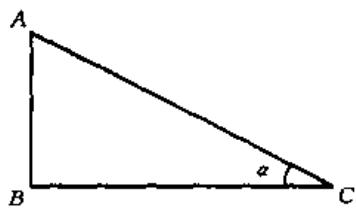
\includegraphics[width=0.3\textwidth]{figures/力图1-1-1.jpg}
\end{center}
\newpage

\textbf{1-2} 一质点以初速度 $v_{0}$ 作直线运动，所受阻力与其速度成正比。试求当质点速度减为 $\dfrac{v_0}{n}$ $(n > 1)$ 时，质点经过的距离与质点所能行经的总距离之比。

\vfill

\textbf{1-3} 一质点以初速度 $v_{0}$ 作直线运动，所受阻力与其速度的三次方成正比。试求质点速度和位置随时间的变化规律以及速度随位置的变化规律。

\vfill

\newpage

\textbf{1-4} 如力图1-4-1，在倾角为 $\theta$ 的山坡平面上有一门大炮，大炮相对于山坡的仰角为 $\alpha$，发射炮弹的初速为 $v_{0}$。试求炮弹着点的位置，并求能达到最大射程的仰角，忽略空气阻力。

\begin{center}
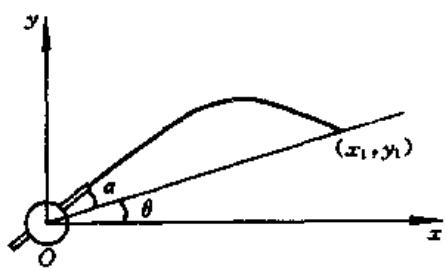
\includegraphics[width=0.3\textwidth]{figures/力图1-4-1.jpg}
\end{center}
\vfill

\textbf{1-5} 两质点在地面上同一地点以相同速率 $v_{0}$ 从不同抛射角抛出。试证明，当两质点的射程 $R$ 相同时，它们在空中飞行时间的乘积为 $\dfrac{2R}{g}$，忽略空气阻力。

\vfill

\textbf{1-6} 如力图1-6-1，位于地面的水枪与一竖直墙的垂直距离为 $d = 3.0\,\mathrm{m}$，墙高 $h = 4.0\,\mathrm{m}$。从水枪喷出初速恒定的水流，为使水流刚好能越过墙顶，试问水流从枪口喷出的初速 $v_{0}$ 的最小值以及水枪的仰角 $\alpha$ 各为多少？忽略空气阻力，重力加速度 $g$ 取 $10\,\mathrm{m/s^2}$。

\begin{center}
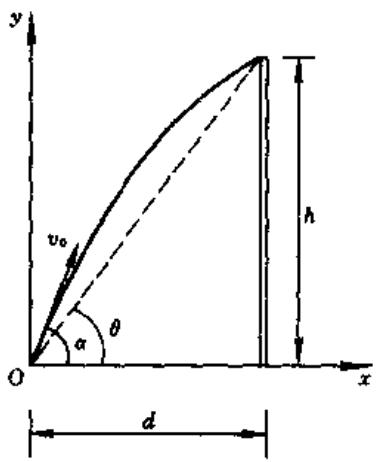
\includegraphics[width=0.3\textwidth]{figures/力图1-6-1.jpg}
\end{center}
\vfill

\newpage

\textbf{1-7} 如力图1-7-1，球1和球2均从同一点水平抛出，起抛点离水平地面的高度为 $H$。两球的水平初速分别为 $v_{1}$ 和 $v_{2}$ $(v_{1} > v_{2})$。球1抛出后刚好能越过位于 $x_{P}$ 处的竖直杆的顶端，并落于地面上的 $R$ 点，$R$ 点与 $O$ 点的距离为 $R$。球2抛出后落于地面，与地面作弹性碰撞，反弹后也刚好越过杆顶，并落在同一点 $R$。试求：1. 比值 $\dfrac{v_1}{v_2}$。2. 杆的位置 $x_{P}$。3. 杆的高度 $h$。

\begin{center}
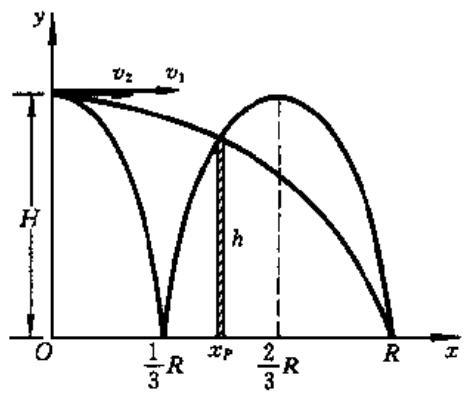
\includegraphics[width=0.3\textwidth]{figures/力图1-7-1.jpg}
\end{center}
\vfill

\textbf{1-8} 飞行物自地面以匀速 $v_{\mathrm{f}}$ 向上空垂直飞行。在地面离飞行物起飞点相距 $L$ 处发射一枚导弹，导弹与飞行物同时发射。导弹的速率 $v$ 为常值，且 $v > v_{\mathrm{f}}$，每一瞬时导弹均指向飞行物运动。

1. 试求导弹的飞行轨迹；

2. 试问导弹经多长时间击中飞行物。

\vfill

\newpage

\textbf{1-9} 圆柱体固定不动，其轴线与水平面垂直。很轻的不可伸长的柔软细线全部缠绕在圆柱体上且在同一水平面内，线末端系一小球，紧贴圆柱体表面。突然给小球一击，使之具有在水平方向并与圆柱体垂直的初速度 $\boldsymbol{v}$，于是缠绕的细线开始从圆柱体上解开。设解开过程中细线与圆柱体之间无相对滑动，且重力可略，即小球始终在水平面内运动。

试求：1. 小球的加速度。2. 小球的轨迹方程。

\vfill

\textbf{1-10} 细杆绕端点 $O$ 在平面内匀角速旋转，角速度为 $\omega$，杆上一小环（可看作质点）相对杆作匀速运动，相对速度为 $v$。设 $t = 0$ 时刻小环位于杆的端点 $O$。

1. 试证明小环的运动轨迹为阿基米德螺线。

2. 试求小环在任意时刻的速度和加速度。

3. 试用作图法定性画出小环加速度在自然坐标系中的两个分量（切向加速度和法向加速度）。

\vfill

\newpage

\textbf{1-11} 如力图1-11-1所示，质点 $A$ 和质点 $B$ 同时从 $A$、$B$ 两点出发，分别以速度 $v_{1}$ 沿 $AB$ 和以速度 $v_{2}$ 沿 $BC$ 作匀速直线运动，$BC$ 和 $AB$ 的夹角为 $\alpha$，开始时质点 $A$ 和质点 $B$ 相距为 $l$，试求两质点之间的最短距离。

\begin{center}
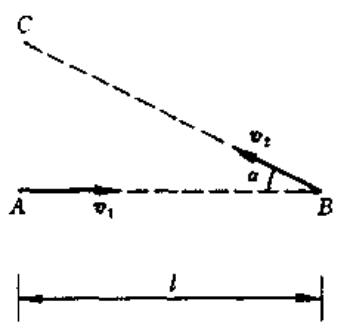
\includegraphics[width=0.2\textwidth]{figures/力图1-11-1.jpg}
\end{center}
\vfill

\textbf{1-12} 宽 $L$ 的河流，流速与离岸的距离成正比，已知两岸处的流速为零，河中心的流速为 $v_{0}$。一小船以恒定的相对速度 $v_{r}$ 垂直于水流从一岸驶向另一岸。在离岸 $\dfrac{L}{4}$ 处因故突然掉头，以相对速度 $\dfrac{v_{r}}{2}$ 垂直于水流驶回本岸。

试求：1. 小船的运动轨迹。2. 小船返回本岸时，所到处与原出发点的距离是多少。

\vfill

\newpage

\textbf{1-13} 如力图1-13-1，一条笔直的河流宽度为 $d$，河水以恒定的速度 $v_{0}$ 流动。小船从河岸的 $A$ 点出发，为了到达对岸的 $O$ 点，相对于河水以恒定的速率 $v^{\prime}$ $(v^{\prime} > v_{0})$ 运动，不论小船驶到何处，它的运动方向总是指向 $O$ 点。已知 $\overline{AO} = r_0$，$\angle AOP = \varphi_0$，试求小船运动的轨迹。若 $O$ 点刚好在 $A$ 点的对面（即 $\overline{AO} = d$），结果又如何？

\begin{center}
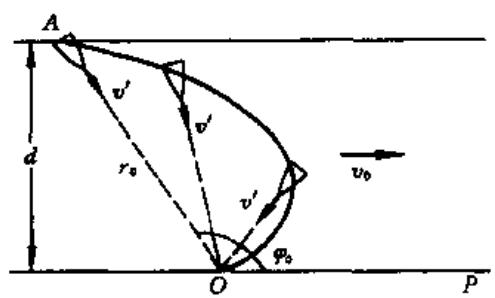
\includegraphics[width=0.3\textwidth]{figures/力图1-13-1.jpg}
\end{center}
\vfill

\textbf{1-14} 如力图1-14-1，轮子在水平面上以角速度 $\omega$ 作纯滚动，已知轮子的质心速度为 $v_{\mathrm{c}}$，试求轮边缘上任一点 $A$ 的绝对速度，$A$ 点的位置用 $\theta$ 角表示。

\begin{center}
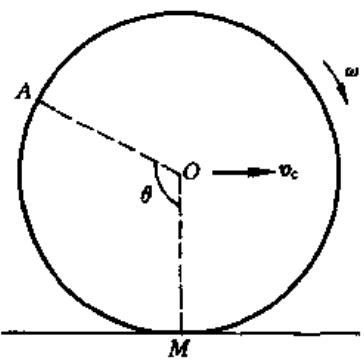
\includegraphics[width=0.3\textwidth]{figures/力图1-14-1.jpg}
\end{center}
\vfill

\newpage

\textbf{1-15} 如力图1-15-1，半径为 $R$ 的圆环静止不动，半径为 $r$ 的圆盘沿圆环内侧作无滑动的滚动，圆盘中心 C 点绕环中心 O 点的角速度恒为 $\Omega$。试求圆盘上与圆环相接触的 A 点相对圆环的加速度。

\begin{center}
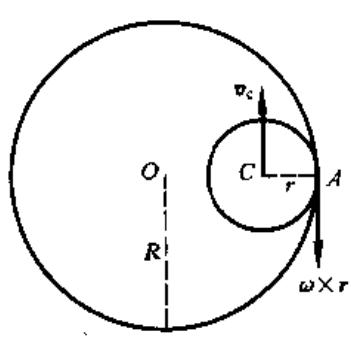
\includegraphics[width=0.2\textwidth]{figures/力图1-15-1.jpg}
\end{center}





\chapter{牛顿运动定律}
\newpage
\textbf{2-1} 如力图2-1-1，在固定不动的圆柱体上绕有绳索，绳两端挂大、小两桶，其质量分别为 $M = 1000\,\mathrm{kg}$ 和 $m = 10\,\mathrm{kg}$。绳与圆柱体之间的摩擦系数为 $\mu = 0.050$，绳的质量可以忽略。试问为使两桶静止不动，绳至少需绕多少圈。

\begin{center}
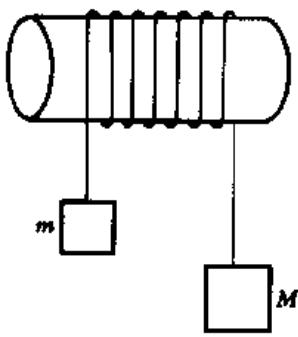
\includegraphics[width=0.15\textwidth]{figures/力图2-1-1.jpg}
\end{center}
\vfill

\textbf{2-2} 如力图2-2-1，细杆一端支在地面上，以恒定的角速度 $\omega$ 绕通过支点的竖直轴旋转，杆与地面的夹角为 $\alpha$，质量为 $m$ 的小环套在杆上，可以沿杆滑动，环与杆之间的摩擦系数为 $\mu$。试问小环处于什么位置上能维持稳定运动。

\begin{center}
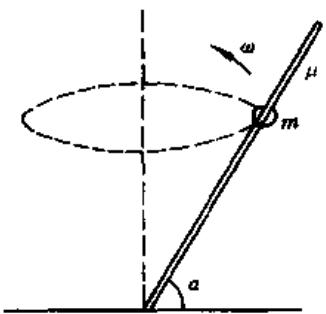
\includegraphics[width=0.15\textwidth]{figures/力图2-2-1.jpg}
\end{center}
\vfill
\newpage

\textbf{2-3} 如力图2-3-1，在半径为 $R$ 的空心球壳内壁，有一可当作质点的小球沿固定的水平圆周作匀速率运动，小球与空心球壳球心的连线与铅垂线的夹角为 $\theta$，小球与空心球壳内壁之间的摩擦系数为 $\mu$。试求小球能稳定运动的速度范围。

\begin{center}
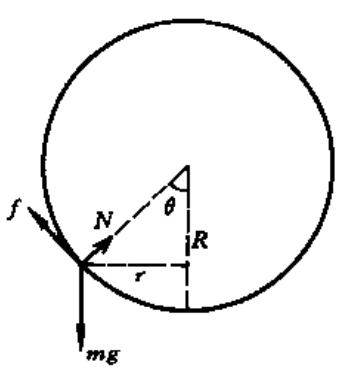
\includegraphics[width=0.15\textwidth]{figures/力图2-3-1.jpg}
\end{center}
\vfill


\textbf{2-4} 如力图2-4-1，在地面上有一倾角为 $\theta$、质量为 $M$ 的斜面体，斜面体上有一质量为 $m$ 的木块，设地面与斜面体之间以及斜面体与木块之间均光滑无摩擦。试求 $M$ 与 $m$ 相对于地面的加速度 $a_{M}$ 与 $a_{m}$，以及木块 $m$ 所受的支持力。

\begin{center}
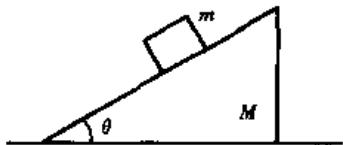
\includegraphics[width=0.3\textwidth]{figures/力图2-4-1.jpg}
\end{center}
\vfill

\newpage

\textbf{2-5} 如力图2-5-1，一个半径为 $R = 0.5\,\mathrm{m}$ 的空心球壳绕本身的竖直直径旋转，角速度为 $\omega = 5\,\mathrm{s^{-1}}$，在空心球壳内高度为 $\dfrac{R}{2}$ 处有一小木块（可当作质点）同球壳一起旋转。

试求：1. 摩擦系数至少是多少才能实现这一情况。2. 当 $\omega = 8\,\mathrm{s^{-1}}$ 时，实现这一情况的条件是什么。3. 研究以下两种情形运动的稳定性：(a) 木块位置有微小变动；(b) 空心球壳的角速度有微小变动。

\begin{center}
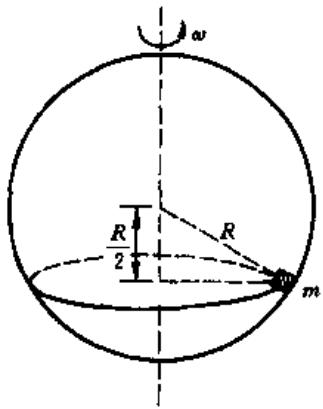
\includegraphics[width=0.15\textwidth]{figures/力图2-5-1.jpg}
\end{center}
\vfill

\textbf{2-6} 如力图2-6-1，一质量为 $m = 20\,\mathrm{kg}$ 的对称钢件，架在两个完全相同的平行长直滚轴上。两滚轴在同一水平面内，滚轴半径为 $r = 0.025\,\mathrm{m}$，绕各自的中心轴以相同的角速度 $\omega = 40\,\mathrm{rad/s}$ 作反向转动。钢件与滚轴间的摩擦系数为 $\mu = 0.20$。为使钢件以 $v_{0} = 0.050\,\mathrm{m/s}$ 的速度沿滚轴作匀速直线运动，需沿滚轴的长度方向对钢件施以水平作用力 $F$，试求 $F$ 的大小。

\begin{center}
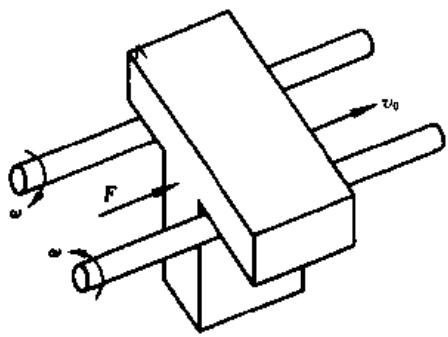
\includegraphics[width=0.15\textwidth]{figures/力图2-6-1.jpg}
\end{center}
\vfill

\newpage

\textbf{2-7} 如力图2-7-1所示，质量分别为 $m_{A}$ 和 $m_{B}$ 的两木块 A 和 B 静止放置在粗糙的水平地面上，两者与地面之间的摩擦系数均为 $\mu$，两木块 A 和 B 的接触面是倾角为 $\theta$ 的斜面，接触面是光滑的。现施一水平推力 $F$ 于 A，使 A 和 B 产生向右的加速度，且 A 和 B 之间不发生相对滑动。试问 $\mu$ 和 $F$ 各应满足什么条件。

\begin{center}
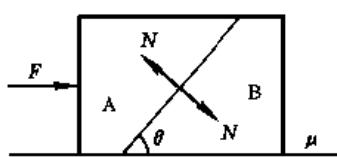
\includegraphics[width=0.2\textwidth]{figures/力图2-7-1.jpg}
\end{center}
\vfill

\textbf{2-8} 如力图2-8-1所示，质量为 $M$ 的滑块C放置在光滑桌面上。质量均为 $m$ 的两个重物 A 和 B 用细绳相连，A 平放在滑块上，与滑块间的摩擦系数为 $\mu$，细绳跨过滑轮后将 B 竖直悬挂。设细绳和滑轮的质量均忽略不计，滑轮转轴不受摩擦力。今以水平推力 $F$ 作用于滑块，为使重物 A 和 B 与滑块保持相对静止，试问 $F$ 至少应多大？

\begin{center}
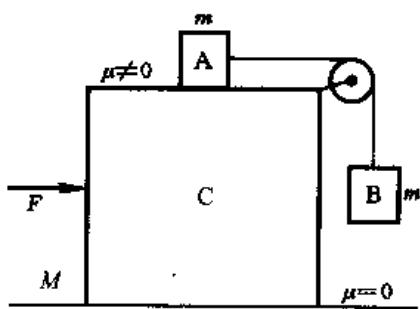
\includegraphics[width=0.2\textwidth]{figures/力图2-8-1.jpg}
\end{center}
\vfill

\newpage

\textbf{2-9} 如力图2-9-1所示，在水平面内有一平台可绕竖直的中心轴以角速度 $\omega$ 匀角速旋转，在平台内沿半径方向有一光滑细槽，槽内放置两质量均为 $m$ 的小球，两球用劲度系数为 $k$、原长为 $a$ 的轻弹簧相连。弹簧的自然长度恰好等于槽的宽度，即两球刚好接触。平台以角速度 $\omega$ 旋转时，两球在槽内离中心的距离分别为 $r_{1}$ 和 $r_{2}$，试求 $r_{1}$ 和 $r_{2}$。

\begin{center}
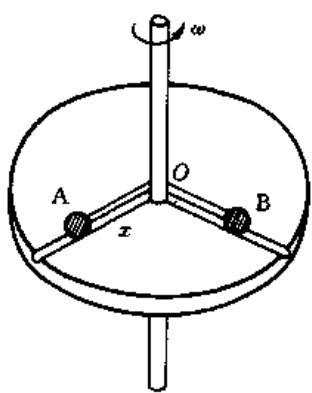
\includegraphics[width=0.2\textwidth]{figures/力图2-9-1.jpg}
\end{center}
\vfill



\textbf{2-10} 质量为 $m$ 的物体以初速 $v_{0}$ 从地面竖直上抛，设空气阻力 $f = \mu v^{2}$，$\mu$ 为常数。试求物体达到的最大高度，并证明物体返回原处的速度为 $v_{0}\sqrt{\dfrac{mg}{mg + \mu v_{0}^{2}}}$。

\vfill

\newpage

\textbf{2-11} 两质点的质量均为 $m$，质点1从离地面高度为 $h$ 处由静止下落，质点2从质点1正下方的地面上以初速 $v_0$ 同时竖直上抛。设空气阻力与质点速率成正比，比例系数为 $\mu$（常量）。试求两质点相遇的时间、地点以及相遇时两质点的速度。

\vfill

\textbf{2-12} 质量为 $m$ 的抛射体初速为 $v_{0}$，抛射角为 $\alpha$，在空气中运动时，所受阻力与速率成正比，比例系数为 $k$。试求轨迹方程，并验证当 $k \to 0$ 时变为抛物方程。

\vfill

\newpage

\textbf{2-13} 飞机以 $v_{0} = 90\,\mathrm{km/h}$ 的水平速度触地滑行着陆。滑行期间受到的空气阻力为 $c_{x}v^{2}$，升力与速度平方成正比，即 $L = c_{y}v^{2}$。已知飞机质量为 $m$，机翼面积为 $S$，升阻比 $K = \dfrac{c_y}{c_x} = 5$，触地瞬间升力与重力恰好平衡。试求飞机触地后的滑行距离 $x$ 和速度随时间的变化关系 $v(t)$。

\vfill

\textbf{2-14} 如力图2-14-1，质量为 $m$ 的小球用一质量可略的弹簧1竖直悬挂起来，弹簧的劲度系数为 $k$。当弹簧的伸长量超过临界长度 $l_{\mathrm{C}}$ $\left(l_{\mathrm{C}} > \dfrac{mg}{k}\right)$ 时，弹簧将被拉断。在小球下方再挂完全相同的另一弹簧2，并在其下端施一与时间 $t$ 有关的拉力 $F(t)$。若以小球在平衡位置时作为计时起点，则拉力随时间变化的关系为 $F(t) = \alpha t$，其中 $\alpha$ 是一恒定参量。试求两弹簧同时被拉断时，参量 $\alpha$ 应满足的关系式。

\begin{center}
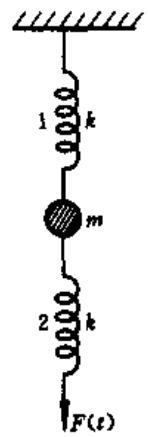
\includegraphics[width=0.08\textwidth]{figures/力图2-14-1.jpg}
\end{center}
\vfill

\newpage

\textbf{2-15} 如力图2-15-1，质量为 $M$、倾角为 $\theta$ 的斜面体放在光滑的桌面上，斜面体上有质量为 $m$ 的木块，木块与斜面体之间的摩擦系数 $\mu < \tan \theta$，以水平力 $F$ 推斜面体，使之运动。试问为了使木块相对于斜面体保持静止，$F$ 的大小应在什么范围。

\begin{center}
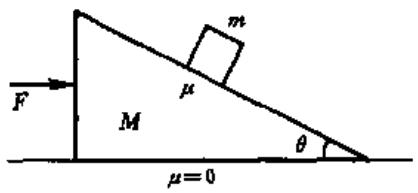
\includegraphics[width=0.25\textwidth]{figures/力图2-15-1.jpg}
\end{center}
\vfill

\textbf{2-16} 如力图2-16-1，地面上有一质量为 $M$、倾角为 $\alpha_{1}$、$\alpha_{2}$ 的斜面体。质量为 $m_{1}$ 和 $m_{2}$ 的两木块分别置于斜面体两侧，用绳经滑轮相连。设地面、斜面、滑轮的摩擦以及绳子和滑轮的质量均可忽略，绳不可伸长，试求 $m_{1}$（或 $m_{2}$）相对 $M$ 的加速度以及 $M$ 的绝对加速度。

\begin{center}
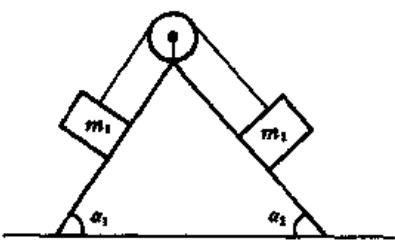
\includegraphics[width=0.25\textwidth]{figures/力图2-16-1.jpg}
\end{center}
\vfill

\newpage

\textbf{2-17} 如力图2-17-1，质量为 $m_{1}$ 的航天飞机A绕地球作匀速圆周运动，轨道半径为 $R$，从航天飞机伸出一长度为 $L$ $(L \ll R)$ 的刚性杆，杆端固定一质量为 $m_{2}$ $(m_{2} \ll m_{1})$ 的卫星S。设A和S均可看作质点，A-S系统的位置用 $\alpha$ 角表示，$\alpha$ 角是杆与A和地心连线之间的夹角。试求A-S系统的平衡位置，并讨论平衡的稳定性。

\begin{center}
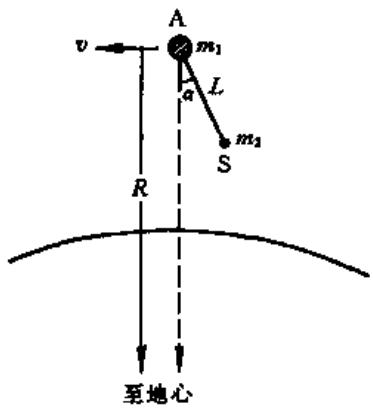
\includegraphics[width=0.2\textwidth]{figures/力图2-17-1.jpg}
\end{center}
\vfill

\textbf{2-18} 如力图2-18-1，半径为 $R$ 的圆盘与水平面平行，绕通过盘中心 $O$ 的竖直轴以角速度 $\omega$ 匀速旋转。盘边缘 $A$ 点处的射手相对于圆盘以水平初速 $v_{0}$ 发射子弹，目标是直径 $AB$ 的另一端点 $B$。设子弹速度远大于盘的转速，且发射子弹不影响圆盘的角速度，设空气阻力可忽略。试问射手应瞄准何方才能击中目标？从射手看来，子弹的轨迹如何？

\begin{center}
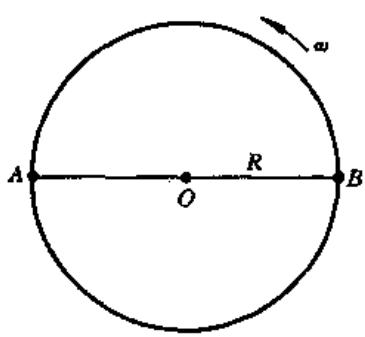
\includegraphics[width=0.2\textwidth]{figures/力图2-18-1.jpg}
\end{center}
\vfill

\newpage

\textbf{2-19} 地球以角速度 $\omega$ 自转，一质点在纬度 $\varphi$ 上空 $h$ 高度处自由下落。忽略空气阻力和惯性离心力。试求因科里奥利力引起的落地点的偏离。

\vfill

\textbf{2-20} 1851年，法国物理学家傅科发现单摆并不在固定的平面内摆动。如果把每次摆动近似看作在一个平面内，并把这个平面称为摆动平面，则摆动平面将以一定角速度作缓慢的顺时针转动（在北半球）。这个现象是由地球的自转造成的，这种摆称为傅科摆。试证明傅科摆摆动平面的旋转周期 $T'$ 与摆所在处的纬度 $\varphi$ 有关，并遵守

\[
T' = \frac{T_0}{\sin\varphi}
\]

式中 $T_0 = \dfrac{2\pi}{\omega}$ 为地球自转周期。




\chapter{功、能和动量}
\newpage
\textbf{3-1} 如力图3-1-1，劲度系数为 $k$ 的弹簧下端竖直悬挂着两个物体，质量分别为 $m_{1}$ 和 $m_2$。达到平衡后，突然撤去 $m_{2}$，试求 $m_{1}$ 运动的最大速度。

\begin{center}
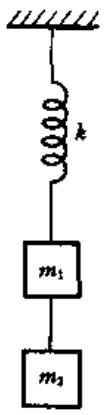
\includegraphics[width=0.05\textwidth]{figures/力图3-1-1.jpg}
\end{center}
\vfill

\textbf{3-2} 如力图3-2-1，水平弹簧一端固定，另一端系一质量为 $m$ 的小球，弹簧的劲度系数为 $k$，小球与水平面之间的摩擦系数为 $\mu$。当弹簧为原长时小球位于 O 点，开始时小球位于 O 点右方的 A 点，O 与 A 之间的距离为 $l_{0}$，从静止释放小球。

1. 为使小球能通过 O 点，而且只能通过 O 点一次，试问 $\mu$ 值应在什么范围？

2. 在上述条件下，小球在 O 点左方的停住点 B 点与 O 点的最大距离 $l_{1}$ 是多少？

\begin{center}
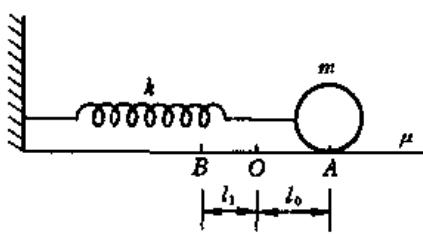
\includegraphics[width=0.25\textwidth]{figures/力图3-2-1.jpg}
\end{center}
\vfill

\newpage
\textbf{3-3} 如力图3-3-1所示，一木块沿倾角 $\theta = 30^{\circ}$ 的斜面从某初始位置以 $v_{0} = 4.5\,\mathrm{m/s}$ 的初速向上运动。已知木块与斜面之间的摩擦系数 $\mu = 0.35$。规定木块初始位置处的重力势能为零。试求木块动能等于重力势能处相对其初始位置的高度。
\begin{center}
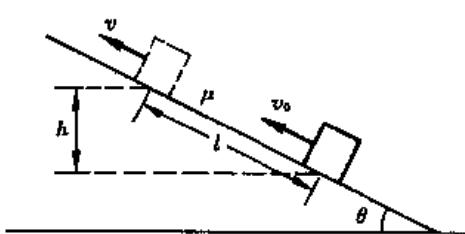
\includegraphics[width=0.15\textwidth]{figures/力图3-3-1.jpg}
\end{center}
\vfill

\textbf{3-4} 如力图3-4-1，在水平桌面上开有一孔，绳子的一部分平放在桌面上，另一部分经孔下垂。设绳不可伸长，均匀柔软，全长为 $l$，下垂长度为 $x_0$，从静止开始下落。设摩擦可略。试求在下落过程中，绳子速度随下落长度变化的规律，以及绳的下端位置随时间变化的规律。
\begin{center}
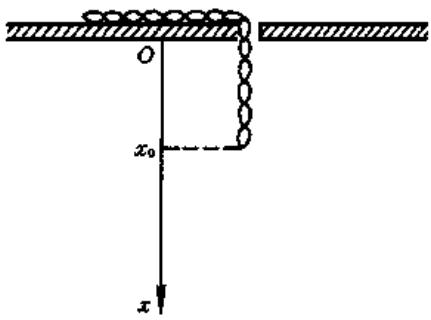
\includegraphics[width=0.15\textwidth]{figures/力图3-4-1.jpg}
\end{center}
\vfill

\newpage
\textbf{3-5} 如力图3-5-1，单摆的摆长为 $L$，摆球质量为 $m$，从左侧与竖直方向夹角 $\alpha$ 处静止下摆。在右侧，与悬点相距为 $r$、与竖直方向夹角为 $\beta$ $(\beta < \alpha)$ 处有一固定的钉子。设空气阻力可略。

试求：1. 为使小球能绕钉子作一个完整的圆周运动，角 $\alpha$ 至少应多大？2. 为使小球能与钉子相碰，角 $\alpha$ 应多大？

\begin{center}
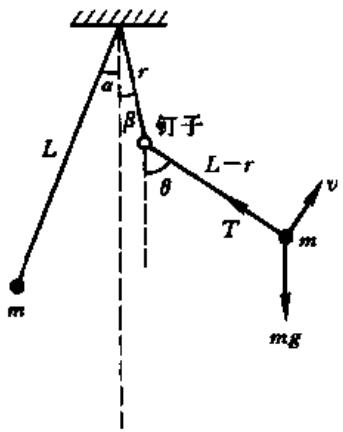
\includegraphics[width=0.2\textwidth]{figures/力图3-5-1.jpg}
\end{center}
\vfill

\textbf{3-6} 如力图3-6-1，质量为 $M$ 的圆环用细线（质量可略）悬挂，圆环上串着两个质量均为 $m$ 的小球，两小球自圆环顶端从静止开始同时向两边滑下，设摩擦可略。

\begin{center}
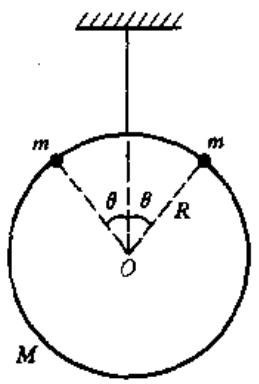
\includegraphics[width=0.15\textwidth]{figures/力图3-6-1.jpg}
\end{center}
\vfill

\newpage
\textbf{3-7} 如力图3-7-1，长为 $2r = 20\,\mathrm{cm}$、质量可以忽略的棒，中心点 $C$ 处有一固定的质量为 $m$ 的质点。棒一端 $A$ 点靠在竖直墙上，另一端 $B$ 点支在地面上，两端可分别沿墙和地面无摩擦地滑动。棒从竖直位置静止下滑，滑动过程中棒始终保持在同一竖直平面内。试求棒中心 $C$ 点触地的位置。

\begin{center}
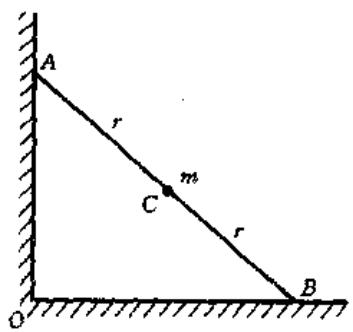
\includegraphics[width=0.2\textwidth]{figures/力图3-7-1.jpg}
\end{center}
\vfill

\textbf{3-8} 如力图3-8-1所示，长为 $L$ 的细杆顶端固定一小重球，竖直倒置在粗糙的水平地面上。小球处于不稳定的平衡状态，稍有扰动，小球将从静止开始向下跌落。假设细杆很轻，其质量可略。试求小球碰地时速度的水平分量和竖直分量。

\begin{center}
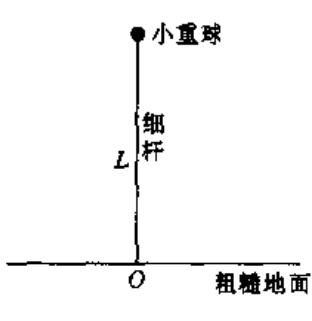
\includegraphics[width=0.2\textwidth]{figures/力图3-8-1.jpg}
\end{center}
\vfill

\newpage
\textbf{3-9} 如力图3-9-1，长为 $2l$ 的不可伸长的细绳一端固定于 $A$ 点的钉子上，另一端系一小球，小球可绕 $A$ 点在铅垂面内运动。开始时小球与 $A$ 点位于同一水平线上，小球在 $A$ 点右侧，垂直向下的初速度为 $v_{0}$。与 $A$ 点在同一水平线上左侧的 $B$ 点也有一钉子，$A$ 与 $B$ 之间的距离为 $l$。当细绳转到 $B$ 点后，小球将绕 $B$ 点向上运动。为使小球能与 $A$ 点的钉子相碰，试问小球初速 $v_{0}$ 的最小值应为多少？
\vfill

\textbf{3-10} 如力图3-10-1所示，在惯性系 $S$ 中有两质点 $A$ 和 $B$，质量分别为 $m_{1}$ 和 $m_{2}$，彼此间以万有引力相互吸引。开始时 $A$ 静止，$A$ 和 $B$ 相距 $l_{0}$，$B$ 以速度 $v_{0}$ 沿连线方向远离 $A$ 而运动 $(v_{0} < \sqrt{\frac{2Gm_2}{l_0}})$，$G$ 为引力常量。$B$ 受一指向其运动方向的变力 $F$ 的作用，使 $B$ 保持速度 $v_{0}$ 不变。

试求：1. 两质点之间的最大距离 $l_{\max}$。2. 从开始到最大距离过程中，变力 $F$ 所作的功（相对于惯性系 $S$）。

\begin{center}
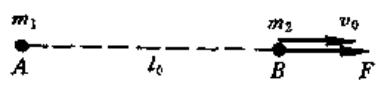
\includegraphics[width=0.3\textwidth]{figures/力图3-10-1.jpg}
\end{center}
\vfill

\newpage
\textbf{3-11} 如力图3-11-1，设想在地球表面的 $A$、$B$ 两地之间开凿一直通隧道，在 $A$ 处放置一小球，小球在地球引力的作用下从静止开始在隧道内运动。忽略一切摩擦阻力。试求小球的最大速度，以及小球从 $A$ 到 $B$ 所需的时间。已知地球半径为 $R$，地球表面的重力加速度为 $g$，$A$ 和 $B$ 之间的直线距离为 $L$。又设地球内部质量密度为恒量。

\begin{center}
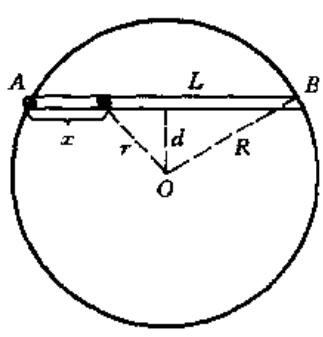
\includegraphics[width=0.2\textwidth]{figures/力图3-11-1.jpg}
\end{center}
\vfill

\textbf{3-12} 如力图3-12-1，两个质量均为 $m$ 的小球串在质量可忽略的光滑细杆上，用两根完全相同的弹簧相连，两弹簧的劲度系数均为 $k$，原长均为 $l_{0}$，左侧弹簧的左端固定在细杆的 $O$ 点，细杆绕 $O$ 点在水平面内转动。
\begin{center}
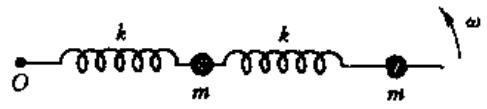
\includegraphics[width=0.15\textwidth]{figures/力图3-12-1.jpg}
\end{center}
\vfill

\newpage
\textbf{3-13} 如力图3-13-1，半径为 $R$ 的光滑圆环绕竖直的直径轴以角速度 $\omega$ 旋转。一质量为 $m$ 的小球串在圆环上，可沿环无摩擦地滑动。试求小球的平衡位置，并讨论平衡的稳定性。
\begin{center}
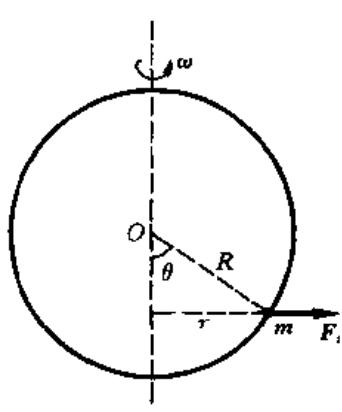
\includegraphics[width=0.15\textwidth]{figures/力图3-13-1.jpg}
\end{center}
\vfill

\textbf{3-14} 如力图3-14-1，在相距为 $l$ 的两平行弹性墙壁之间，有质量为 $m$ 的弹性小球以垂直于壁的初速度 $v_{0}$ 往返弹跳，设壁的质量远大于 $m$，碰撞是完全弹性的，重力及空气阻力可略。

试求：1. 每壁所受的平均作用力。2. 若用外力使左壁以速度 $V$ $(V \ll v_{0})$ 缓缓右移，证明外力作功等于小球动能的增加。
\begin{center}
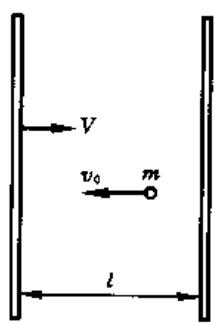
\includegraphics[width=0.15\textwidth]{figures/力图3-14-1.jpg}
\end{center}
\vfill

\newpage
\textbf{3-15} 如力图3-15-1，$A$、$B$、$C$ 三质点静止放置在光滑水平面上，它们的质量分别为 $m_{1}$、$m_{2}$、$m_{3}$，用柔软、不可伸长、质量可略的绳子相连并拉直，$AB$ 与 $BC$ 的夹角为 $\alpha$。以沿 $BC$ 方向的冲量 $I$ 作用于 $C$，试求质点 $A$ 开始运动时的初速。

\begin{center}
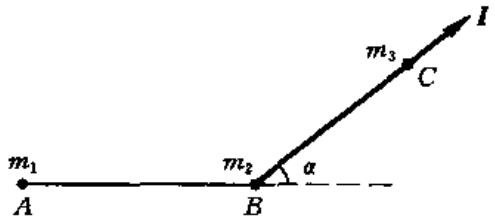
\includegraphics[width=0.2\textwidth]{figures/力图3-15-1.jpg}
\end{center}
\vfill

\textbf{3-16} 如力图3-16-1，从地面发射的炮弹在达到最高点处炸裂为质量相等的两块。第一块在炸裂后沿原方向运动，第二块则沿水平方向被弹出。已知炮弹发射的初速为 $v_0$，发射角为 $\theta$。忽略空气阻力，炸裂后第二块的落地点距发射点的水平距离为 $S_1$。试求第一块落地点距发射点的水平距离 $S_2$。

\begin{center}
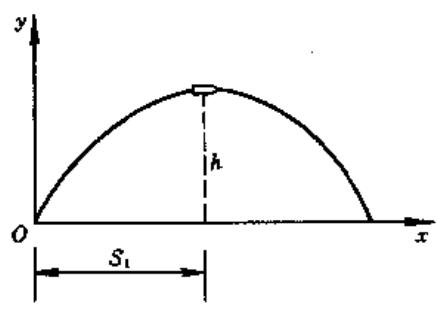
\includegraphics[width=0.2\textwidth]{figures/力图3-16-1.jpg}
\end{center}
\vfill

\newpage
\textbf{3-17} 地面上静止放置着质量为 $M$ 的平板车，车上有 $N$ 个人，每个人的质量均为 $m$。每个人以相同的相对速度 $u$（相对跳后的车速）沿水平方向从车后跳离平板车。忽略一切阻力。试问，在 $N$ 个人同时跳出和逐个跳出两种情况下，平板车在哪种情况下获得的动能大。
\vfill

\textbf{3-18} 如力图3-18-1，地面上有质量为 $M$、倾角为 $\theta$ 的斜面体，其顶端高 $h$ 处有质量为 $m$ 的小木块。开始时两者均静止，然后小木块从斜面体顶端滑至底部。忽略各种摩擦及阻力。试求：以地面为参考系，在小木块下滑过程中斜面体的支持力对它所作的功。

\begin{center}
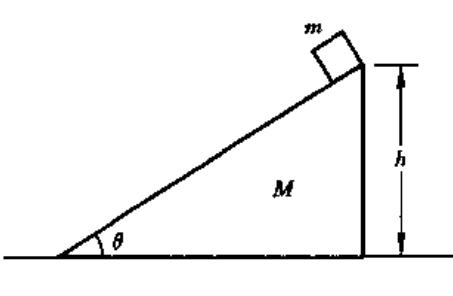
\includegraphics[width=0.2\textwidth]{figures/力图3-18-1.jpg}
\end{center}
\vfill

\newpage
\textbf{3-19} 如力图3-19-1，地面上静止地放置着质量为 $M$ 的木块，其底部为平面，上部有截面为半圆的凹槽，半径为 $R$，质量为 $m$ 的小球从最高处静止下滑。设各种摩擦及阻力均可略。试求：1. 在小球 $m$ 下滑过程中，$m$ 的绝对速度 $v$、$M$ 的绝对速度 $v_{M}$ 以及 $m$ 的相对速度 $v^{\prime}$ 随小球位置 $\theta$ 的变化规律。2. 小球 $m$ 在最低点时给木块 $M$ 的压力。

\begin{center}
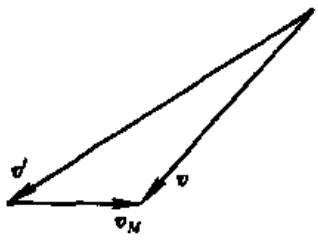
\includegraphics[width=0.2\textwidth]{figures/力图3-19-1.jpg}
\end{center}
\vfill

\textbf{3-20} 如力图3-20-1，质量为 $m_{3}$ 的木块平放在地面上，通过劲度系数为 $k$ 的竖直弹簧与质量为 $m_{2}$ 的木块相联，达到平衡。质量为 $m_{1}$ 的小球从距 $m_{2}$ 为 $h$ 的高处静止下落，与 $m_{2}$ 作完全非弹性碰撞。试问：为使 $m_{2}$ 向上反弹时能带动 $m_{3}$ 刚好离开地面，$h$ 应为多少？

\begin{center}
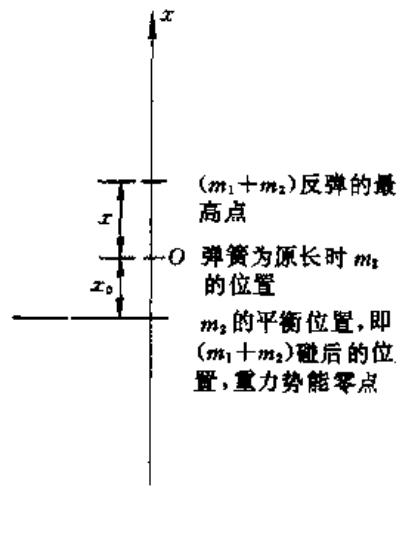
\includegraphics[width=0.25\textwidth]{figures/力图3-20-1.jpg}
\end{center}
\vfill

\newpage
\textbf{3-21} 如力图3-21-1所示，质量为 $M$ 的长滑块静止地放在光滑的水平桌面上，一质量可略的弹簧固定在滑块左端，弹簧的劲度系数为 $k$，滑块右端用一不可伸长的细绳固定在竖直墙上，细绳能承受的最大拉力为 $T_{0}$。一质量为 $m$，初速为 $v_{0}$（其方向水平向左）的小物在滑块上无摩擦地向左滑动，最终与弹簧相碰并压缩弹簧。
\begin{center}
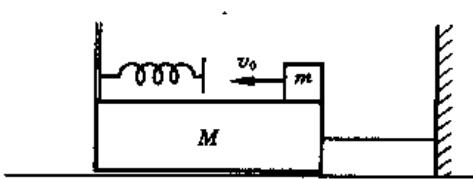
\includegraphics[width=0.2\textwidth]{figures/力图3-21-1.jpg}
\end{center}
\vfill

\textbf{3-22} 如力图3-22-1，球1和球2的质量分别为 $m_{1}$ 和 $m_{2}$，放置在光滑水平地面上，球1以一定的水平初速 $v_{10}$ 向右沿两球连心线运动，球2则静止。两球连心线右侧有一竖直弹性墙。设两球之间以及球与墙之间的所有碰撞均为完全弹性碰撞。为了使两球能发生、而且只能发生两次碰撞，试问两球的质量之比 $\dfrac{m_1}{m_2}$ 应满足什么条件？
\begin{center}
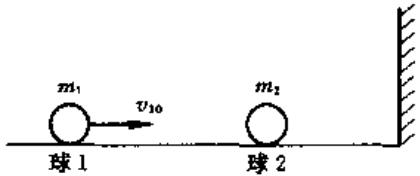
\includegraphics[width=0.2\textwidth]{figures/力图3-22-1.jpg}
\end{center}
\vfill

\newpage
\textbf{3-23} 如力图3-23-1，两根长度均为 $l$ 的刚性细杆，一端用质量为 $m$ 的球形铰链相连，两杆另一端分别安装质量为 $m$ 和 $2m$ 的小球。开始时两杆并拢，铰链球朝上，竖直放置在光滑桌面上，从静止释放，下面两球开始向两边滑动，两杆始终保持在同一铅垂面内。设三球本身的大小、轻杆的质量以及各种摩擦均可忽略。

\begin{center}
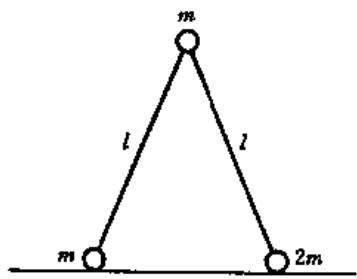
\includegraphics[width=0.2\textwidth]{figures/力图3-23-1.jpg}
\end{center}
\vfill

\textbf{3-24} 小球从高度为 $h$ 处静止下落，与地面碰撞时的恢复系数为 $e$。忽略空气阻力，忽略碰撞过程所需时间。
\vfill

\newpage
\textbf{3-25} 如力图3-25-1，台阶每级的宽和高均为 $l$。一小球向下逐级弹跳，每次反弹后，相对本级达到的最高高度均为 $H$，每次的下落点均在各级的同一地点。已知小球与台阶碰撞时的恢复系数为 $e$，忽略空气阻力。

\begin{center}
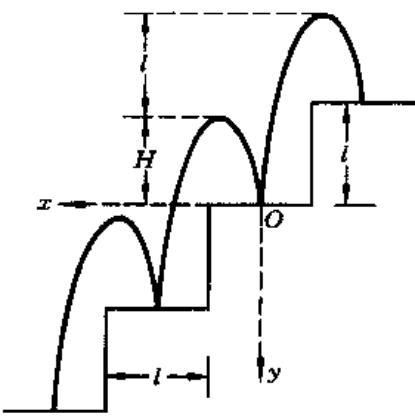
\includegraphics[width=0.2\textwidth]{figures/力图3-25-1.jpg}
\end{center}
\vfill

\textbf{3-26} 如力图3-26-1，在固定斜面的 $O$ 点上方 $h = 1.60\,\mathrm{m}$ 处有一小球从静止自由下落。已知斜面是光滑的，倾角为 $\theta = 15^{\circ}$，小球与斜面碰撞时的恢复系数为 $e = 0.60$，忽略空气阻力。

试求：1. 小球碰后达到的最高点与 O 点之间的高度差 $h_{\max}$。2. 设小球碰后落在斜面上 P 点，则 O 点与 P 点的距离 $S$ 是多少？3. 小球与斜面碰撞后，其机械能损失的百分数是多少？

\begin{center}
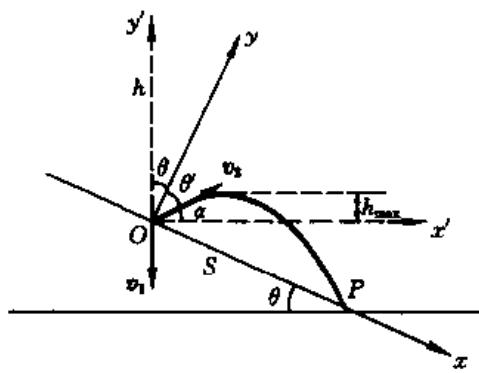
\includegraphics[width=0.3\textwidth]{figures/力图3-26-1.jpg}
\end{center}
\vfill

\newpage
\textbf{3-27} 如力图3-27-1，质量为 $M$ 的斜面体静止放置在光滑的水平桌面上，斜面体的倾角 $\theta = 15^{\circ}$。质量为 $m$ 的小球由静止自由下落到斜面体上，下落高度 $h = 1.60\,\mathrm{m}$。设斜面体表面是光滑的，并知小球碰后和碰前相对斜面体的相对速度在垂直于斜面方向的分量之比为 $e = 0.60$，碰撞点离桌面高度 $H = 1.00\,\mathrm{m}$，$M = 2m$。
\begin{center}
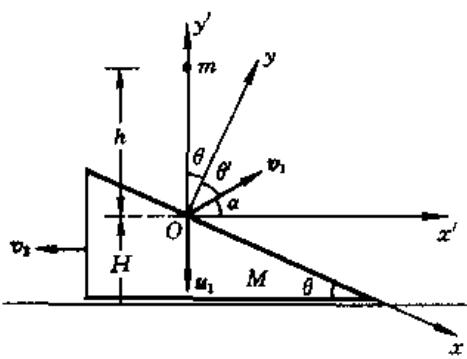
\includegraphics[width=0.2\textwidth]{figures/力图3-27-1.jpg}
\end{center}
\vfill

\textbf{3-28} 一平板放置在光滑水平桌面上，一小球在此桌面上运动并与平板作完全弹性碰撞，设小球也是光滑的。试证明：不论平板原来静止或处于运动状态，相对平板而言，小球总是遵守入射角等于反射角的规律。
\vfill

\newpage
\textbf{3-29} 如图3-29-1，均匀圆环静止放置在光滑水平桌面上，圆环质量为 $M$，半径为 $R$。一质量为 $m$ 的质点以速度 $v_0$ 沿圆环的直径方向射向圆环，碰撞是完全弹性的。试求碰后圆环的运动状态和质点的运动状态。
\begin{center}
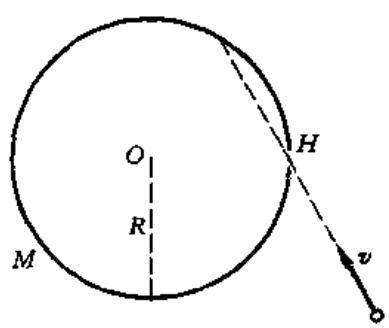
\includegraphics[width=0.2\textwidth]{figures/图3-29-1.jpg}
\end{center}
\vfill

\textbf{3-30} 三质点的质量分别为 $m_{1}$、$m_{2}$、$m_{3}$，以万有引力相互作用，绕垂直于三质点所在平面并通过质心 C 的转轴旋转。

试问：为使三质点的相对位置保持不变，需满足什么条件？
\vfill

\newpage
\textbf{3-31} 质量为 $M$ 的平板车静止在光滑地面上，车上有 $N$ 个人，每人的质量均为 $m$，若每人消耗同样的体力（即每人作功相同）沿水平方向向后跳，忽略空气阻力，人可看作是质点。
\vfill

\textbf{3-32} 如力图3-32-1，质量分别为 $m_{1}$ 和 $m_{2}$ 的两木块用劲度系数为 $k$ 的弹簧相连，静止地放在光滑地面上。质量为 $m$ 的子弹以水平初速 $v_{0}$ 射入木块 $m_{1}$，设子弹射入过程的时间极短。
\begin{center}
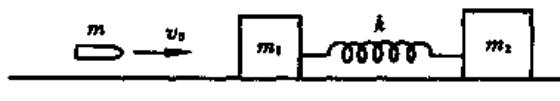
\includegraphics[width=0.2\textwidth]{figures/力图3-32-1.jpg}
\end{center}
\vfill

\newpage
\textbf{3-33} 如力图3-33-1，在光滑地面上静止地放着质量为 $m$ 的箱子。在箱内光滑的底面上，质量也为 $m$ 的滑块以水平初速 $v_{0}$ 开始运动，并与两壁反复碰撞。已知滑块与箱子每碰一次后，两者的相对速度改变 $e = \sqrt[4]{\frac{1}{2}}$ 倍。

试求：1. 最多经几次碰撞后，系统总能量的损耗不大于40\%。2. 从滑块开始运动到完成上述次数的碰撞后，箱子的平均速度是多少？
\begin{center}
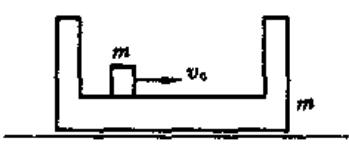
\includegraphics[width=0.2\textwidth]{figures/力图3-33-1.jpg}
\end{center}
\vfill

\textbf{3-34} 动能为 $E_0$ 的 ${}^4\mathrm{He}$ 核轰击静止的 ${}^7\mathrm{Li}$ 核，作完全非弹性碰撞后成为复合核 ${}^{11}\mathrm{B}$，${}^{11}\mathrm{B}$ 进一步分裂为 ${}^{10}\mathrm{B}$ 和中子 ${}^1\mathrm{n}$。上述核反应过程需消耗能量 $Q = 2.8\,\mathrm{MeV}$。反应方程为
\[
{}^4\mathrm{He} + {}^{7}\mathrm{Li} \rightarrow ({}^{11}\mathrm{B}) \rightarrow {}^{10}\mathrm{B} + {}^{1}\mathrm{n} - 2.8\,\mathrm{MeV}
\]

试求：上述核反应过程所需的 $E_{0}$ 的最小值是多少？相应的中子动能为多大？
\vfill

\newpage
\textbf{3-35} 一物体作直线运动，其质量不断随时间变化。设该物体在 $t$ 时刻的质量为 $M(t)$，速度为 $v(t)$。试证明下述密舍尔斯基方程：
\[
M\frac{\mathrm{d}v}{\mathrm{d}t} = (u - v)\frac{\mathrm{d}M}{\mathrm{d}t} + F
\]

式中 $F$ 是质量不断变化的主体所受的合外力，$u$ 是附加物附加到主体前的绝对速度或抛出物抛离主体后的绝对速度。
\vfill

\textbf{3-36} 竖直下垂的绳子从静止自由下落，开始时绳下端刚好与地面接触。设绳均匀柔软，全长为 $l$。

试证明：下落过程中地面所受压力等于已经落在地面上的绳子重量的3倍。
\vfill

\newpage
\textbf{3-37} 火箭从地面竖直向上发射。已知火箭自身质量为 $M_{s}$，燃料的初始质量为 $M_{f}$，燃气相对火箭的喷射速度为 $v^{\prime}$，单位时间的喷气质量为 $a$。设在火箭上升的高度范围内 $g$ 为常量，忽略空气阻力。

试求：1. 火箭的推力和加速度。2. 任意时刻火箭的速度和上升高度。3. 燃料耗尽时，火箭的加速度、速度和高度。4. 火箭能达到的最大高度及所需时间。
\vfill

\textbf{3-38} 如力图3-38-1，质量为 $m$ 的小球下系一条足够长的柔软均匀且不可伸长的绳子。绳子的质量线密度为 $\lambda$。将小球以初速 $v_{0}$ 从地面竖直上抛，忽略空气阻力。

试问：在上升过程中，小球的速率怎样随高度变化？
\begin{center}
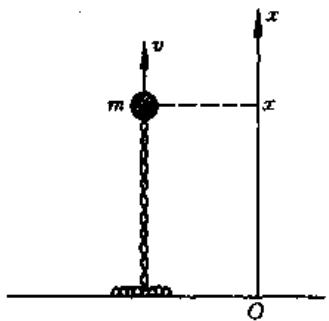
\includegraphics[width=0.25\textwidth]{figures/力图3-38-1.jpg}
\end{center}
\vfill

\newpage
\textbf{3-39} 球状小水滴在静止的雾气中下落，下落过程中吸附了全部所遇到的水分子。设水滴始终保持球状，设雾气密度均匀，忽略空气的粘滞力，重力加速度取恒定值 $g$。

试证明经过足够长时间后，水滴加速度趋于稳定值，并求出此稳定值。
\vfill



\chapter{角动量、有心运动}
\newpage
\textbf{4-1} 试根据牛顿万有引力定律证明开普勒行星运动三定律。
\vfill

\textbf{4-2} 已知行星绕太阳沿椭圆轨道运动（开普勒第一定律）。试证明行星所受太阳引力必定与距离平方成反比。
\vfill

\newpage
\textbf{4-3} 如力图4-3-1，设质量为 $M$ 的恒星固定不动。质量为 $m$ 的行星在其引力作用下运动，运动轨迹可以是椭圆、抛物线或双曲线。试求各种轨迹相应的总能量，并给出各种轨迹的判据。

\begin{center}
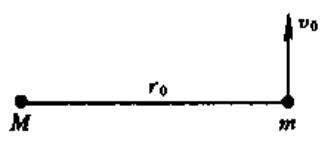
\includegraphics[width=0.25\textwidth]{figures/力图4-3-1.jpg}
\end{center}
\vfill

\textbf{4-4} 空间两质点的质量分别为 $m_{1}$ 和 $m_{2}$，彼此以万有引力相互作用。开始时两质点静止，相距 $r_0$，在引力作用下彼此接近并相碰。试求两质点从开始运动到相碰所经历的时间。
\vfill

\newpage
\textbf{4-5} 如力图4-5-1所示，质量为 $m = 1.20 \times 10^{4}\,\mathrm{kg}$ 的飞船在离月球表面高度为 $h = 100\,\mathrm{km}$ 处绕月球作圆周运动。飞船采用两种登月方式。1. 在 A 点向前（即向力图4-5-1上方）短时间喷气，使飞船与月球相切地到达月球上的 B 点（AB 通过月球中心 O 点）。2. 在 A 点向外侧（即向力图4-5-1右方）沿月球半径短时间喷气，使飞船与月球相切地到达月球上的 C 点（CO 与 AB 垂直）。设喷气相对飞船的速度为 $u = 1.00 \times 10^{4}\,\mathrm{m/s}$。已知月球半径 $R = 1700\,\mathrm{km}$，月球重力加速度（当作常量）$g = 1.700\,\mathrm{m/s^2}$。试求：两种登月方式各需的燃料质量。

\begin{center}
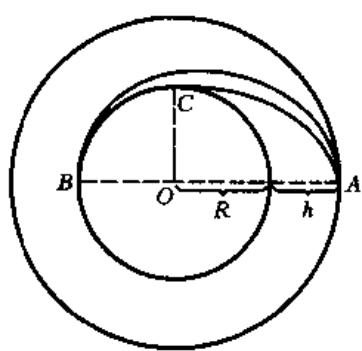
\includegraphics[width=0.2\textwidth]{figures/力图4-5-1.jpg}
\end{center}
\vfill

\textbf{4-6} 如力图4-6-1，飞船绕地球作圆周运动，离地面的高度 $h = 800\,\mathrm{km}$，地球半径 $R = 6.40 \times 10^{3}\,\mathrm{km}$，飞船圆轨道半径 $r_{0} = R + h$，飞船速度 $v_{0} = 3.00 \times 10^{4}\,\mathrm{km/h}$。经过短暂的沿矢径向外侧喷气，飞船获得了指向地心 $O$ 的附加速度 $v_{r} = 800\,\mathrm{km/h}$，其轨道变为椭圆。设喷气后飞船的质量可看作不变。试求：飞船椭圆轨道的近地点和远地点离地面的高度。
\begin{center}
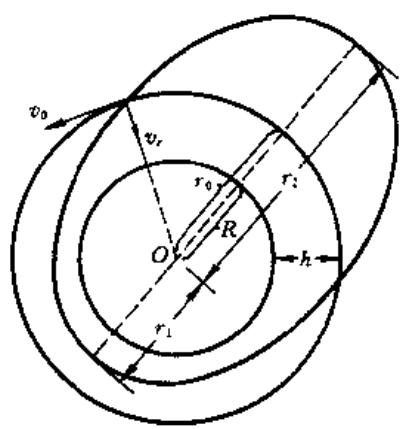
\includegraphics[width=0.2\textwidth]{figures/力图4-6-1.jpg}
\end{center}
\vfill

\newpage
\textbf{4-7} 如力图4-7-1，飞船总质量为 $m$，内装质量为 $m_0$ 的探测器，绕地球沿椭圆轨道运行，近地点与地心距离为 $r_1$，速度为
\[
v_{1} = \sqrt{\frac{2\alpha GM}{r_1}}
\]

1. 试证明 $1 > \alpha > \dfrac{1}{2}$。

2. 如力图4-7-2，飞船在近地点向前发射探测器，并使探测器沿抛物线轨道运动。发射后，飞船沿圆轨道运行。试求：质量比 $\dfrac{m_0}{m}$ 及发射探测器的相对速度 $u$。

3. 如力图4-7-3，若在远地点以上述相对速度 $u$ 发射探测器，试求探测器运行的轨道。

\begin{center}
    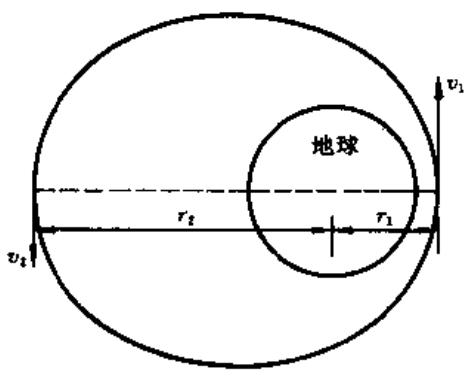
\includegraphics[width=0.16\textwidth]{figures/力图4-7-1.jpg}
    \qquad
    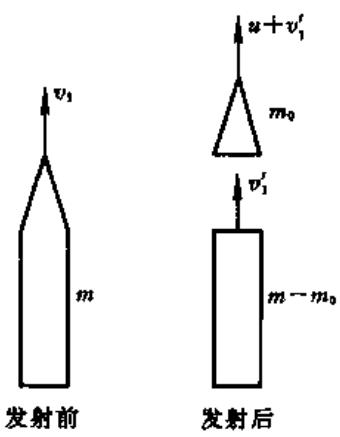
\includegraphics[width=0.16\textwidth]{figures/力图4-7-2.jpg}
    \qquad
    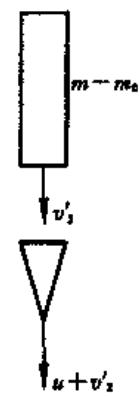
\includegraphics[width=0.08\textwidth]{figures/力图4-7-3.jpg}
\end{center}
\vfill

\textbf{4-8} 如力图4-8-1，地球沿半径为 $R_0$ 的圆轨道绕太阳运动。彗星绕太阳沿抛物线运动。已知抛物线与地球圆轨道一直径的两端相交。忽略地球与彗星之间的引力。

试求：1. 彗星抛物线轨道的方程。2. 彗星的最大速率是地球公转速率的几倍？3. 彗星在地球轨道内的运行时间是多少地球年？
\begin{center}
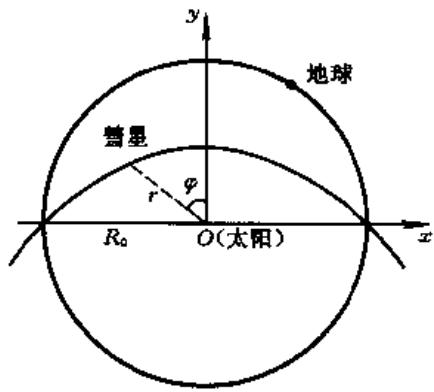
\includegraphics[width=0.2\textwidth]{figures/力图4-8-1.jpg}
\end{center}
\vfill

\newpage
\textbf{4-9} 如力图4-9-1，质量为 $M$ 的宇航站和与其对接上的质量为 $m$ 的飞船一起绕地球沿圆轨道运动，轨道半径是地球半径 $R$ 的 $n$ 倍，$n = 1.25$。某一瞬时，宇航站将飞船沿运动方向发射出去。发射后，飞船和宇航站将分别沿各自新的椭圆轨道运行。已知飞船椭圆轨道的远地点离地球中心的距离为 $8nR$。设发射飞船后宇航站的质量不变（即忽略喷气的质量）。

试问：当质量比 $\dfrac{m}{M}$ 为何值时，飞船绕地球一周后刚好与宇航站相遇。
\begin{center}
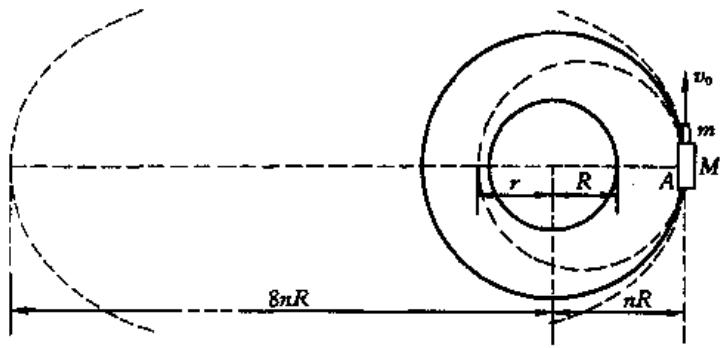
\includegraphics[width=0.3\textwidth]{figures/力图4-9-1.jpg}
\end{center}
\vfill

\textbf{4-10} 如力图4-10-1，从地球发射火箭到火星进行探测，发射后火箭绕太阳沿椭圆轨道运行。为了节省能量，火箭离开地球的速度方向与地球绕太阳公转的速度方向一致，并且选择适当的发射时机，使火箭椭圆轨道的远日点为火星，近日点为地球。假定地球和火星均绕太阳作圆周运动，圆轨道半径分别为 $r_{\text{地}}$ 和 $r_{\text{火}}$，忽略其他行星对火箭的引力作用。

试问：1. 火箭应以多大的相对速度离开地球？2. 火箭到达火星要用多长时间？
\begin{center}
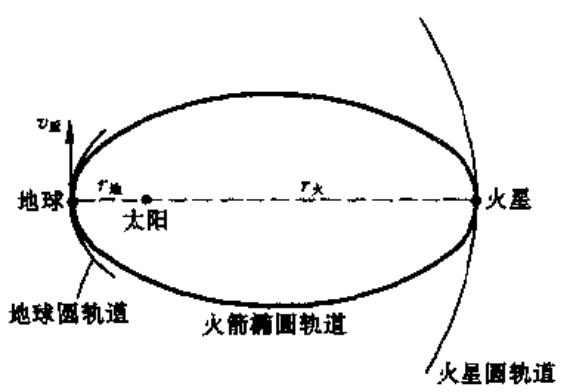
\includegraphics[width=0.3\textwidth]{figures/力图4-10-1.jpg}
\end{center}
\vfill

\newpage
\textbf{4-11} 如力图4-11-1，宇宙飞船绕火星沿圆轨道运行，运动速度为 $v_{0}$。已知火星半径为 $R$，飞船圆轨道离火星表面的高度为 $H$。今飞船在极短时间内，沿圆轨道径向向外侧点火喷气，使飞船获得指向火星的径向速度 $\alpha v_{0}$，$\alpha$ 是远小于1的常数。因喷气量很小，喷气后飞船的质量可视为不变。喷气后，飞船绕火星沿新的椭圆轨道运行。

试求：1. 飞船椭圆轨道近火星点距火星表面的高度 $h_{A}$ 以及远火星点距火星表面的高度 $h_{B}$。2. 飞船绕椭圆轨道的运行周期。
\begin{center}
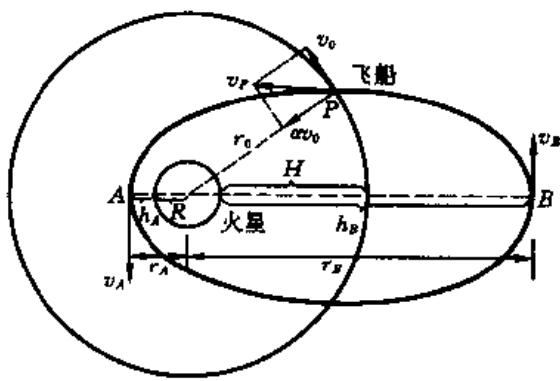
\includegraphics[width=0.3\textwidth]{figures/力图4-11-1.jpg}
\end{center}
\vfill

\newpage

\textbf{4-12} 将宇宙飞船从地面发射到太阳系外，有两个方案。方案一：以足够大的速度（大于太阳系逃逸速度）直接发射。方案二：使宇宙飞船接近太阳系的一个外层行星（例如火星），在它的作用下，改变运动方向，然后逃离太阳系。

试求：1. 按方案一，确定从地面发射飞船所必需的相对地球的最小速度 $v_{a}$ 及发射方向。2. 按本题第1问的方向相对地球以 $v_{b}$ 从地面发射飞船，求飞船穿过火星轨道的速度，即求飞船速度在火星轨道的切线分量和垂直分量。设飞船穿过火星轨道时，火星离飞船很远。3. 使飞船进入火星引力场，但仍可飞出太阳系，求从地面发射的速度。设飞船相对地球的发射方向与本题第一问相同，设飞船沿火星轨道的切线方向脱离火星引力场。4. 估计方案二比方案一节省能量的最大百分比。

设所有行星在同一平面内以同一方向绕太阳在圆轨道上运行。设空气阻力及地球自转的影响均可忽略。

数据：地球绕太阳公转的速度为 $30\,\mathrm{km/s}$，地球到太阳的距离与火星到太阳的距离之比为 $2{:}3$，地球半径 $R_E = 6400\,\mathrm{km}$，地球表面的重力加速度 $g = 9.80\,\mathrm{m/s^2}$。
\vfill

\newpage
\textbf{4-13} 如力图4-13-1，劲度系数 $k = 3$ 的弹簧一端 $O$ 固定，另一端有质量 $m = 20\,\mathrm{g}$ 的质点。质点绕 $O$ 点在光滑水平面内作匀速圆周运动，总机械能为 $E_0 = 12\,\mathrm{J}$。突然沿径向给质点一击，使之获得沿径向向外的速度 $v_{r0} = 1.0\,\mathrm{m/s}$。设弹簧的原长很小，可忽略不计。

1. 试用能量曲线 $(E \sim r)$ 描述质点受打击前、后的运动状态。2. 试求质点运动的半径范围。

\begin{center}
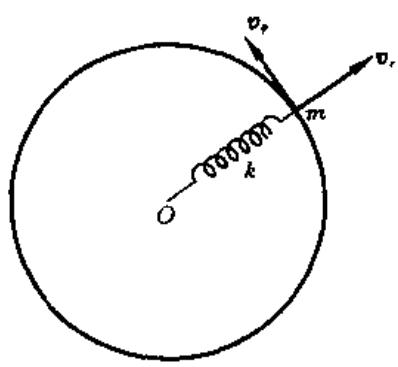
\includegraphics[width=0.2\textwidth]{figures/力图4-13-1.jpg}
\end{center}
\vfill

\textbf{4-14} 一质量为 $m$ 的行星绕质量为 $M$ 的恒星运动。设在行星与恒星之间的整个空间内均匀分布着稀薄的宇宙尘埃，已知尘埃的密度为 $\rho$ 且很小，可以忽略行星与尘埃之间的直接碰撞作用。

1. 试问，对于角动量为 $L$ 的圆形行星轨道，其半径 $r_0$ 应满足什么方程（列出方程即可，不必求解）？

2. 考虑相对上述圆轨道稍有偏离的另一轨道，试解释它是一条作进动的椭圆轨道，进动方向与行星运行方向相反，并求出进动的角速度。
\vfill



\chapter{静力平衡}
\newpage
\textbf{5-1} 如力图5-1-1，静止的圆锥体竖直放置，顶角为 $\alpha$。质量为 $m$ 且分布均匀的链条环水平地套在圆锥体上，忽略链条与圆锥体之间的摩擦力。试求链条中的张力。

\begin{center}
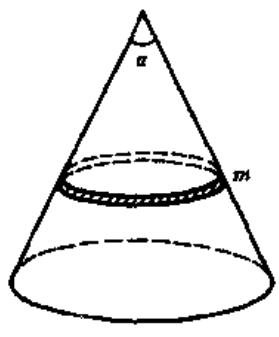
\includegraphics[width=0.15\textwidth]{figures/力图5-1-1.jpg}
\end{center}
\vfill

\textbf{5-2} 如力图5-2-1，均匀杆 $AB$ 长 $l$，重 $w_0$，$A$ 端与粗糙的竖直墙接触，$B$ 端用不可伸长的绳悬挂于竖直墙的 $C$ 点，杆呈水平状态，绳与杆的夹角为 $\theta$。

试问：1. 为了使杆达到静力平衡，杆 A 端与竖直墙之间的摩擦系数 $\mu$ 应满足什么条件？2. 若在杆上悬挂另一重量为 $w = \dfrac{w_0}{2}$ 的重物，为了使杆仍维持平衡，所需摩擦系数的最小值与悬点的位置有何关系？

\begin{center}
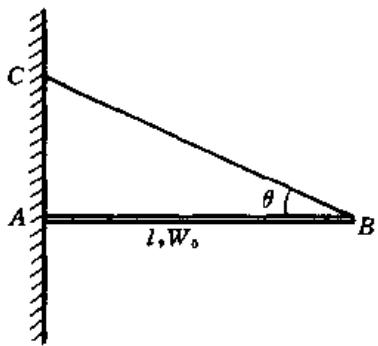
\includegraphics[width=0.2\textwidth]{figures/力图5-2-1.jpg}
\end{center}
\vfill

\newpage
\textbf{5-3} 如力图5-3-1，质量为 $m$、长为 $L$ 的均匀细直杆竖直放置，杆下端与地面之间的摩擦系数为 $\mu$，杆上端用绳索拉住，绳与直杆之间的夹角为 $\theta$。在离地面高度为 $h$ 处以水平力 $F$ 作用于直杆。试问为使直杆不滑倒，作用力 $F$ 的最大值应是多少？

\begin{center}
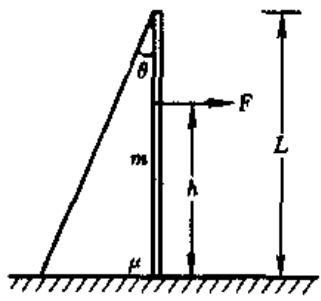
\includegraphics[width=0.2\textwidth]{figures/力图5-3-1.jpg}
\end{center}
\vfill

\textbf{5-4} 如力图5-4-1，在半径为 $R$ 的光滑半球形凹面内，有一刚性均匀细杆达到平衡。已知杆在半球面内那部分的长度为 $l$。试求杆露出半球面外那部分的长度。
\begin{center}
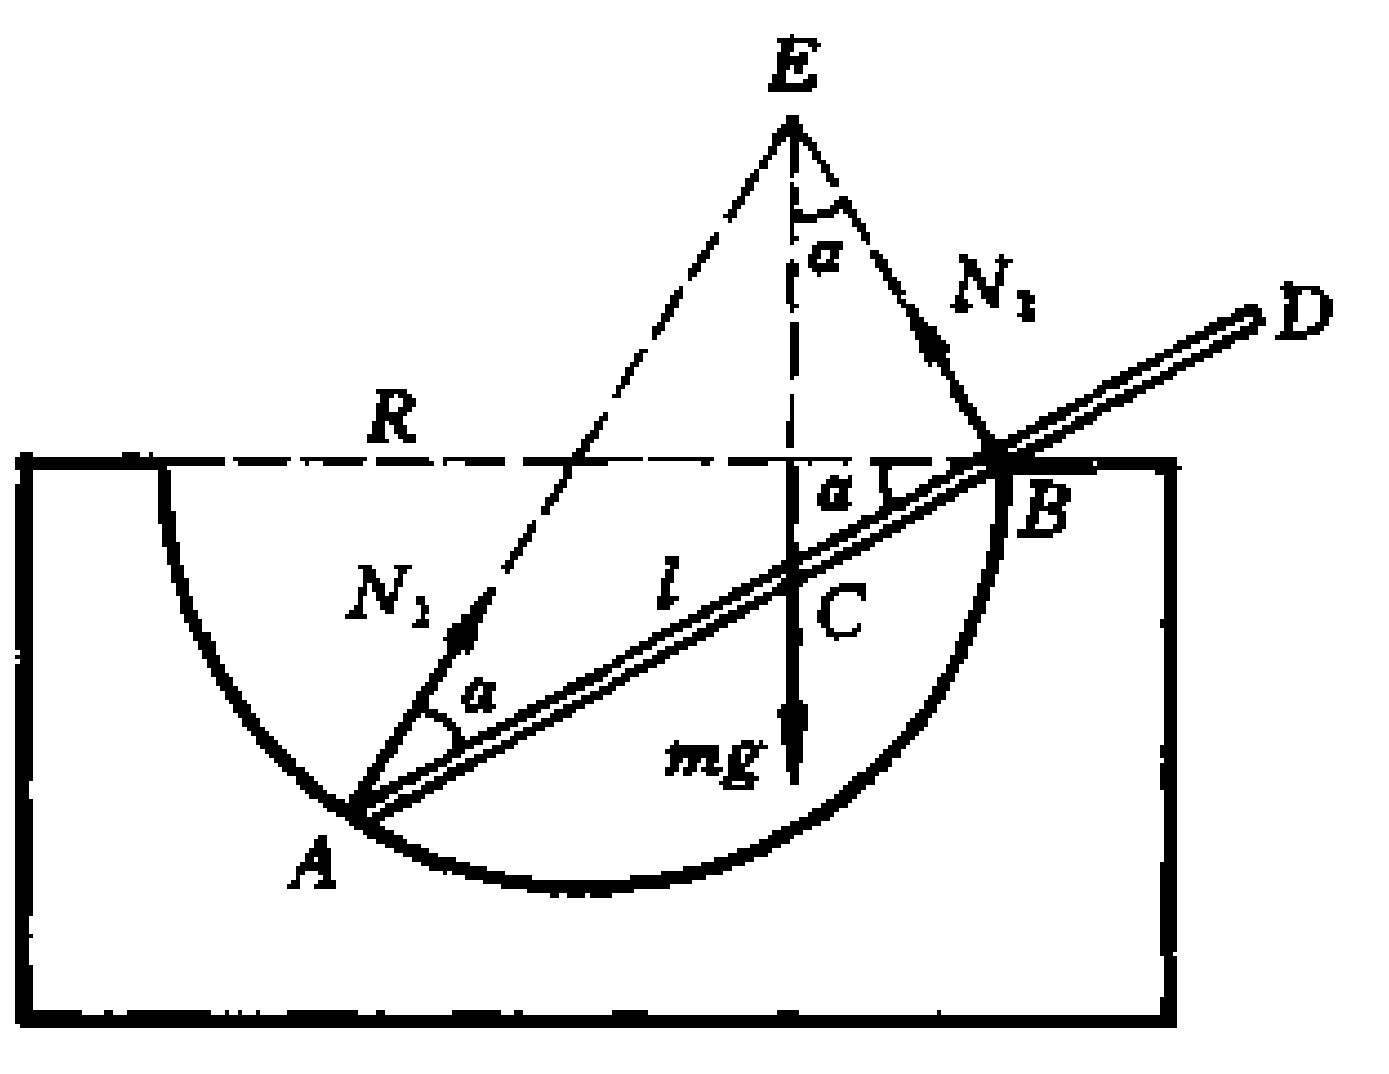
\includegraphics[width=0.2\textwidth]{figures/力图5-4-1.jpg}
\end{center}
\vfill

\newpage
\textbf{5-5} 如力图5-5-1，三个半径和质量均相同的圆柱体按图中的方式堆放在地面上，互相接触。已知圆柱体之间的摩擦系数为 $\mu_{1}$，圆柱体与地面之间的摩擦系数为 $\mu_{2}$。试求使三圆柱体达到平衡所需之 $\mu_{1}$ 和 $\mu_{2}$ 的下限值。

\begin{center}
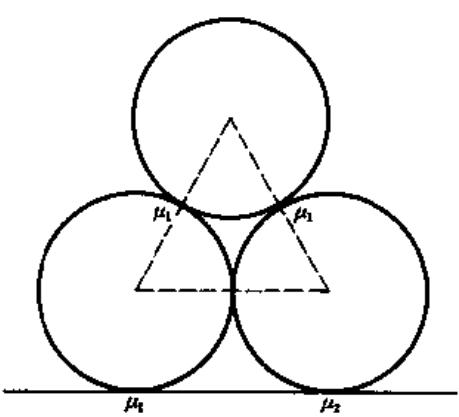
\includegraphics[width=0.2\textwidth]{figures/力图5-5-1.jpg}
\end{center}
\vfill

\textbf{5-6} 如力图5-6-1所示，均匀木板 $AB$ 长 $L = 100\,\mathrm{cm}$，重 $2G$，一端用铰链固定于竖直墙，另一端用水平线拉住，木板与竖直墙之间的夹角为 $60^{\circ}$。三个完全相同的球按力图5-6-1中的位置放在木板上，球半径均为 $R = 10\,\mathrm{cm}$，重量均为 $G$。设球与墙，球与木板，球与球之间的摩擦力均可忽略。试求水平线的拉力 $T$。

\begin{center}
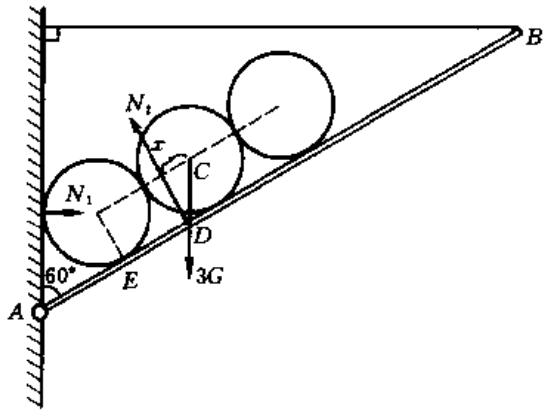
\includegraphics[width=0.3\textwidth]{figures/力图5-6-1.jpg}
\end{center}
\vfill

\newpage
\textbf{5-7} 如力图5-7-1所示，AB、BC、CD和DE为质量可略的等长细线，长度均为 $5\,\mathrm{m}$，$A$ 端和 $E$ 端悬挂在水平天花板上，$AE = 14\,\mathrm{m}$。B 和 D 是质量均为 $m_0 = 7\,\mathrm{kg}$ 的相同小球。质量为 $m$ 的重物挂于 $C$ 点，平衡时 $C$ 点离天花板的垂直距离为 $7\,\mathrm{m}$。

1. 试求质量 $m$。2. 今用外力将 $C$ 点缓慢提升，使BCD位于同一水平线上，试求此过程中外力作的功。

\begin{center}
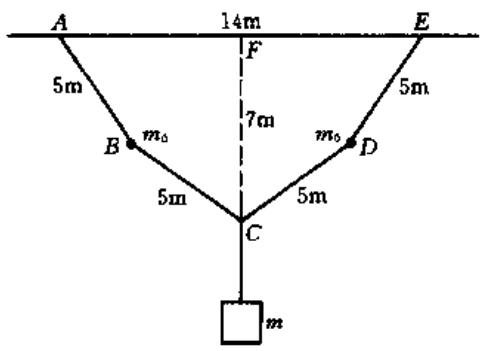
\includegraphics[width=0.2\textwidth]{figures/力图5-7-1.jpg}
\end{center}
\vfill

\textbf{5-8} 如力图5-8-1所示，浮子由两个半径为 $R$ 的球冠相合而成，其质量为 $m_{1}$，中心厚度为 $h$ $(h < 2R)$。长为 $l$，质量为 $m_{2}$ 的均匀细杆从浮子中心垂直插入，下端刚好到达下球冠表面。细杆的铅垂位置显然是一个平衡位置。试分析平衡的稳定性。

\begin{center}
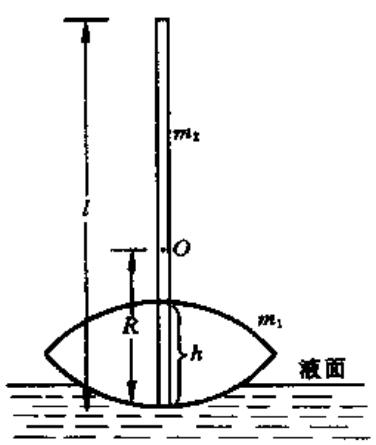
\includegraphics[width=0.2\textwidth]{figures/力图5-8-1.jpg}
\end{center}
\vfill

\newpage
\textbf{5-9} 如力图5-9-1，五根质量分布均匀、质量和长度完全相同的细杆，用光滑铰链互相连结并悬挂起来。试求平衡时由细杆组成的五边形的五个顶角。

\begin{center}
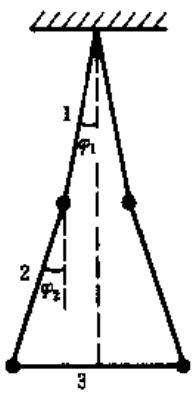
\includegraphics[width=0.12\textwidth]{figures/力图5-9-1.jpg}
\end{center}
\vfill

\textbf{5-10} 如力图5-10-1，半径为 $R$ 的圆柱体在水平面上固定不动，厚度为 $t$ 的均匀木板水平地放置在圆柱体上，其长度方向（力图5-10-1中的横向）与圆柱体的轴（水平方向与力图5-10-1的平面垂直）垂直，并处于平衡状态。试问厚度 $t$ 取何值时属稳定平衡。

\begin{center}
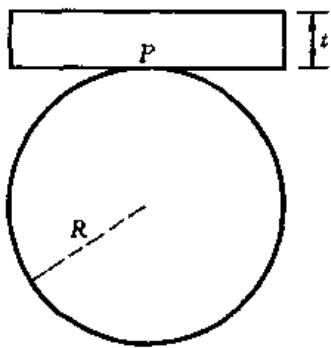
\includegraphics[width=0.2\textwidth]{figures/力图5-10-1.jpg}
\end{center}
\vfill

\newpage
\textbf{5-11} 如力图5-11-1，四根质量、长度都相同的均匀木条用光滑铰链连接成菱形，一均匀圆盘静止地夹在两木条之间，整个系统竖直悬挂起来，悬点为 $O$ 点。设圆盘与木条之间的接触是光滑的。已知每根木条的长度 $l = 50\,\mathrm{cm}$，质量 $m = 50\,\mathrm{g}$；圆盘的半径 $r = 8\,\mathrm{cm}$，质量 $M = 200\,\mathrm{g}$。试求系统的平衡位置（用 $\theta$ 角表示）。
\begin{center}
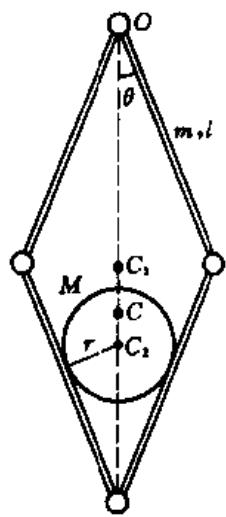
\includegraphics[width=0.1\textwidth]{figures/力图5-11-1.jpg}
\end{center}
\vfill

\textbf{5-12} 如力图5-12-1，质量分布均匀的柔软细绳全长 $L$，质量线密度为 $\lambda$，悬挂在两根竖直杆上，测得细绳在两悬挂点的切线与竖直杆之间的夹角分别为 $\theta_{1}$ 和 $\theta_{2}$。

1. 试求细绳两端所受的拉力。2. 若左悬点的高度为 $H$，试导出在 $Oxy$ 坐标系中的悬链线方程。

\begin{center}
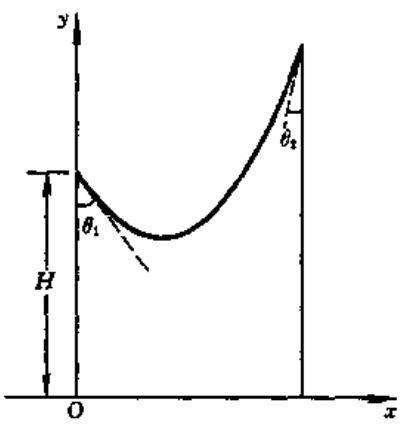
\includegraphics[width=0.18\textwidth]{figures/力图5-12-1.jpg}
\end{center}
\vfill




\chapter{刚体动力学}
\newpage
\textbf{6-1} 汽车在后轮的推动下，以加速度 $a$ 在地面上沿直线前进。已知汽车前轮与后轮的间距为 $2l$，质心位于前后轮的中央，离地高度为 $h$，后轮与地面之间的摩擦系数为 $\mu$，前轮为非驱动轮，与地面的摩擦可略。试问：$\mu$ 至少为多大时，后轮不致打滑？

\begin{center}
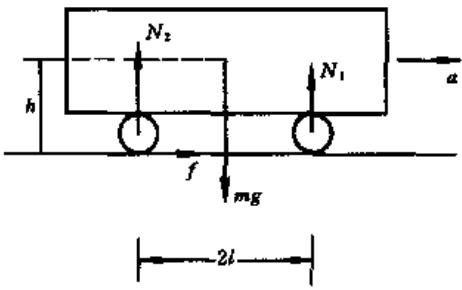
\includegraphics[width=0.2\textwidth]{figures/力图6-1-1.jpg}
\end{center}
\vfill

\textbf{6-2} 如力图6-2-1，质量为 $m$ 的均匀圆柱体，截面半径为 $R$，长为 $2R$。试求：圆柱体绕通过质心及两底面边缘的转轴的转动惯量。

\begin{center}
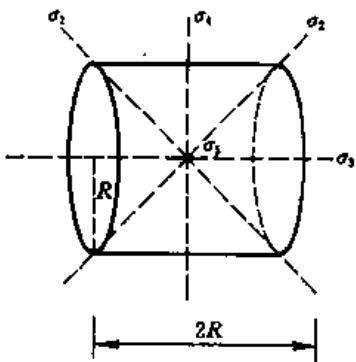
\includegraphics[width=0.2\textwidth]{figures/力图6-2-1.jpg}
\end{center}
\vfill

\newpage
\textbf{6-3} 如力图6-3-1，长为 $l$ 的均匀细杆水平地放置在桌面上，质心离桌边缘的距离为 $b$，从静止下落。已知杆与桌边缘之间的摩擦系数为 $\mu$。试求杆开始滑动时的角度 $\theta_C$。

\begin{center}
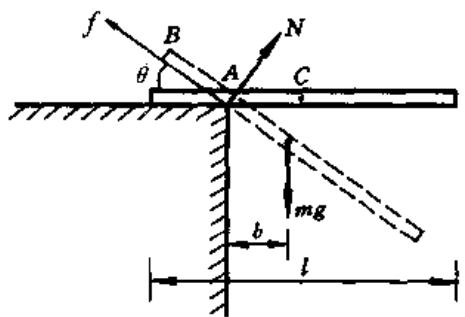
\includegraphics[width=0.2\textwidth]{figures/力图6-3-1.jpg}
\end{center}
\vfill

\textbf{6-4} 如力图6-4-1，实心圆柱体从桌边由静止下滚，圆柱体与桌边之间的摩擦系数为 $\mu$。圆柱体下滚过程中所转过的角度用 $\theta$ 表示。试求圆柱体开始相对桌边滑动时相应角度 $\theta$ 所满足的关系式，并用图解法在图上标出这个角度以及不滑动的转角范围。

\begin{center}
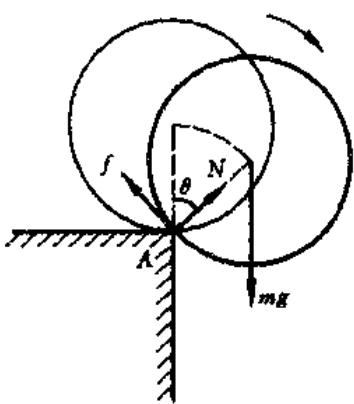
\includegraphics[width=0.2\textwidth]{figures/力图6-4-1.jpg}
\end{center}
\vfill

\newpage
\textbf{6-5} 如力图6-5-1，均匀细麦杆长 $l$，可绕通过中心 $O$ 的固定水平轴在铅垂面内自由转动。开始时麦杆静止于水平位置。一质量与麦杆相同的甲虫以速度 $v_{0}$ 垂直落到麦杆的 $\dfrac{1}{4}$ 长度处，落下后立即向端点爬行。

试问：1. 为使麦杆以均匀的角速度转动，甲虫沿麦杆爬行的速度应是多少？2. 甲虫轨迹的参变方程是什么？3. 为了使甲虫在麦杆转到铅直位置前能爬到端点，甲虫下落速度 $v_{0}$ 的最高值是多少？

\begin{center}
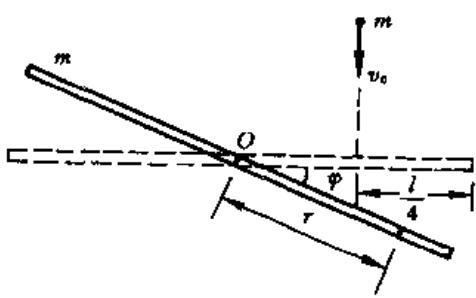
\includegraphics[width=0.2\textwidth]{figures/力图6-5-1.jpg}
\end{center}
\vfill

\textbf{6-6} 如力图6-6-1，半径为 $R$ 的均匀实心圆柱体在水平地面上作纯滚动，其中心 $O$ 点的速度为 $v_{0}$，它向前滚动时遇到一个高为 $h$ 的台阶，并发出完全非弹性碰撞。设圆柱和台阶前缘之间的摩擦系数足够大。

试问：1. $v_{0}$ 为何值时圆柱体能不脱离 A 点而滚上台阶继续前进？2. 对台阶高度 $h$ 有什么限制？

\begin{center}
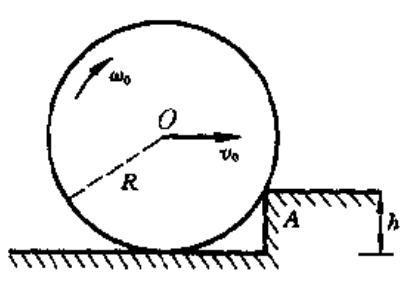
\includegraphics[width=0.2\textwidth]{figures/力图6-6-1.jpg}
\end{center}
\vfill

\newpage

\textbf{6-7} 如力图6-7-1，地球和月球的质量分别为 $M_{E}$ 和 $M_{m}$ ,两者中心的距离用 r 表示,月球可看作质点．设地球的自转轴和月球绕地球作圆周运动的转轴重合，都通过地球中心，地球和月球的角速度分别为 $\omega_{E}$ 和 $\omega_{m}$ ．由于潮汐运动，地球自转角速度会发生微小变化，从而地球和月球的间距以及地球和月球系统的总能量也将发生变化．

1. 试证明, 地球和月球间距的时间变化率 $\dot{r}$ 与地球自转角速度的时间变化率 $\omega_{E}$ 的关系为

$$
\dot {r} = - \frac {2 \sqrt {r} I _ {\mathrm{E}}}{M _ {\mathrm{m}} \sqrt {G M _ {\mathrm{E}}}} \dot {\omega} _ {\mathrm{E}}
$$

式中 $I_{E}$ 是地球对自转轴的转动惯量, G 是引力常量.

2. 试导出地球和月球系统机械能时间变化率的表达式。

3. 设现在的地球与月球间距为 $r(0)$ , 地球的自转角速度为 $\omega_{\mathrm{E}}(0)$ , 受扰动后相应的量变为 $r(t)$ 和 $\omega_{\mathrm{E}}(t)$ , 因扰动很小, 月球仍作圆周运动. 试证明

$$
\omega_ {\mathrm{E}} (t) = \omega_ {\mathrm{E}} (0) - \frac {M _ {\mathrm{m}} \sqrt {G M _ {\mathrm{E}}}}{I _ {\mathrm{E}}} [ \sqrt {r (t)} - \sqrt {r (0)} ]
$$

试计算地球和月球间距增加2\%时, 地球日将变成多少小时.

\begin{center}
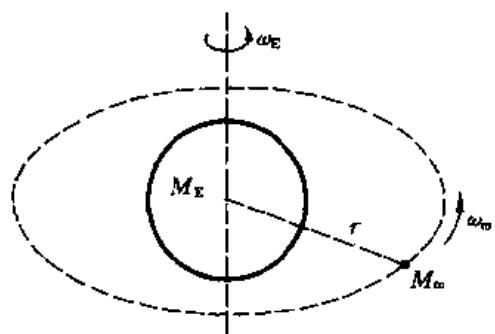
\includegraphics[width=0.25\textwidth]{figures/力图6-7-1.jpg}
\end{center}
\vfill
\newpage

\textbf{6-8} 某行星相对其质心轴的转动惯量为 $I$ ，自转角速度为 $\Omega$ 。质量为 $m$ 的卫星（可看作质点）绕该行星沿圆轨道运动，轨道半径为 $r$ ，角速度为 $\omega$ ，假定两种角速度的方向一致。

1. 一般情形下 $\Omega$ 与 $\omega$ 并不相等, 由于行星上的潮汐摩擦, 行星自转角速度将发生变化, 卫星的圆运动角速度也将相应地改变, 试求两种角速度的改变量之间的关系.

2. 潮汐摩擦将引起行星与卫星系统机械能的损耗, 试问在什么情形下系统机械能可达稳定值.
\vfill


\textbf{6-9} 如力图6-9-1，一线轴质量为 $m$ ，绕质心轴的转动惯量为 $I$ ，大小半径分别为 $R$ 和 $r$ ，轴上绕线，以力 $F$ 拉线，拉力方向与水平面的夹角用 $\theta$ 表示。线轴放置在水平桌面上，与桌面之间的摩擦系数为 $\mu$ ，试讨论线轴的运动情况。

\begin{center}
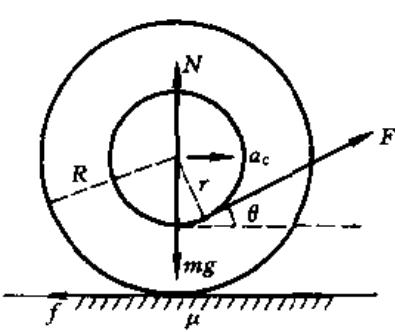
\includegraphics[width=0.2\textwidth]{figures/力图6-9-1.jpg}
\end{center}
\vfill
\newpage

\textbf{6-10} 如力图6-10-1，在 $\alpha = 30^{\circ}$ 的斜面上，质量 $m_{2} = 4\mathrm{kg}$ 的木块经轻绳与质量 $m_{1} = 8\mathrm{kg}$ 半径 $r = 5\mathrm{cm}$ 的实圆柱体的转轴相连。已知斜面的摩擦系数 $\mu = 0.2$ ，圆柱体轴承中的摩擦可以忽略。试求物体的加速度 $a$ ，并讨论加速度 $a$ 、张力 $T$ 、圆柱体所受摩擦力 $f_{1}$ 随斜面倾角 $\alpha$ 的变化。

\begin{center}
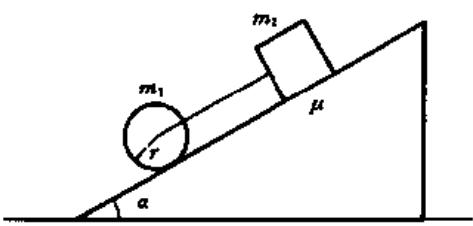
\includegraphics[width=0.25\textwidth]{figures/力图6-10-1.jpg}
\end{center}
\vfill


\textbf{6-11} 如力图6-11-1，半径为 $R$ 的乒乓球，绕质心轴的转动惯量 $I = \frac{2}{3} mR^2, m$ 为乒乓球的质量，以一定的初始条件在粗糙的水平面上运动。开始时球的质心速度为 $v_{\mathrm{C0}}$ ，初角速度为 $\omega_0$ ，两者的方向如图所示。已知乒乓球与地面之间的摩擦系数为 $\mu$ 。试求乒乓球开始作纯滚运动所需的时间及纯滚时的质心速度。

\begin{center}
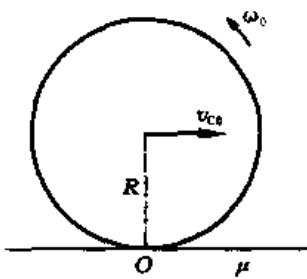
\includegraphics[width=0.2\textwidth]{figures/力图6-11-1.jpg}
\end{center}
\vfill
\newpage

\textbf{6-12} 如力图6-12-1，实心圆柱体从高度为 $h$ 的斜坡上从静止纯滚动地到达水平地面上, 继续纯滚动, 与光滑竖直墙作完全弹性碰撞后返回, 经足够长的水平距离后重新作纯滚动, 并纯滚动地爬上斜坡. 设地面与圆柱体之间的摩擦系数为 $\mu$ , 试求圆柱体爬坡所能达到的高度 $h'$ .

\begin{center}
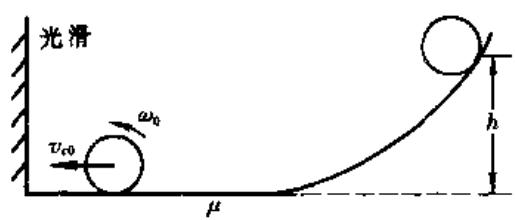
\includegraphics[width=0.3\textwidth]{figures/力图6-12-1.jpg}
\end{center}
\vfill

\textbf{6-13} 如力图6-13-1，实心均匀小球自圆柱面的顶端从静止下滚.

1. 为了保证在 $\varphi \leqslant 45^{\circ}$ 的范围内小球作纯滚动, 试问摩擦系数 $\mu$ 至少应为多少.

2. 设 $\mu = 0.7$ , 试求纯滚结束时小球的质心速度 $v_{1}$.

3. 试求小球从圆柱面脱离时小球的位置 (用 $\varphi$ 角表示) 所满足的方程 (不必求解).

\begin{center}
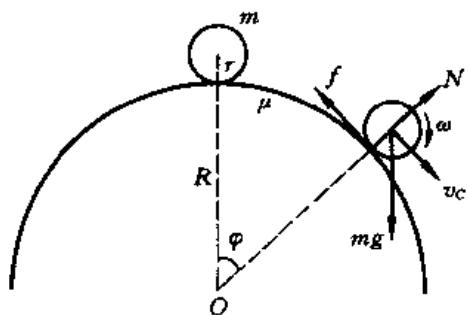
\includegraphics[width=0.25\textwidth]{figures/力图6-13-1.jpg}
\end{center}
\vfill
\newpage

\textbf{6-14} 在水平地面上有两个完全相同的均匀实心球，其一作纯滚动，质心速度为 $v$ ，另一静止不动。两球作完全弹性碰撞，因碰撞时间很短，碰撞过程中摩擦力的影响可以忽略不计。

试求: 1. 碰后两球达到纯滚时的质心速度. 2. 全部过程中损失的机械能的百分数.
\vfill


\textbf{6-15} 如力图6-15-1，两个质量和半径均相同的实心圆柱轮，它们的质心轴互相平行，并用一轻杆相连，轴与轴承间的摩擦忽略不计。两轮先以共同的初速 $v_{0}$ 沿水平方向运动，两轮的初角速度为零。然后同时轻轻与地面相接触。设两轮与地面之间的摩擦系数分别为 $\mu_{1}$ 和 $\mu_{2}(\mu_{1}>\mu_{2})$ 。试求两轮均变为纯滚动所需的时间及纯滚后的平动速度。

\begin{center}
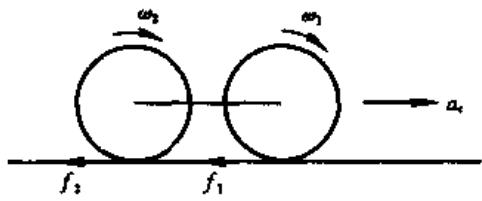
\includegraphics[width=0.3\textwidth]{figures/力图6-15-1.jpg}
\end{center}
\vfill
\newpage

\textbf{6-16} 如力图6-16-1，一半径为 $R$ 的实心均匀球，开始时质心静止，但绕通过质心的水平轴以角速度 $\omega_{0}$ 旋转，在重力作用下垂直下落到地面，球上最低点离地面的高度为 $h$。球与地面碰撞的恢复系数为 $e$，球与地面之间的摩擦系数为 $\mu$ ，忽略空气阻力及碰撞时产生的形变。

1. 试求碰地后球的质心速度和自转角速度。

2. 试求第一次落地点与第二次落地点之间的水平距离。

3. 试画出碰后球的质心速度与地面夹角 $\theta$ 的正切与初始角速度 $\omega_0$ 的关系曲线。

\begin{center}
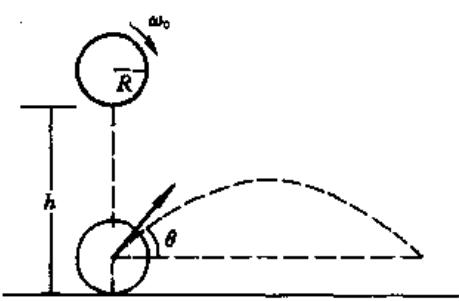
\includegraphics[width=0.25\textwidth]{figures/力图6-16-1.jpg}
\end{center}
\vfill


\textbf{6-17} 如力图6-17-1，斜面体放置在光滑水平面上，斜面倾角为 $\theta$ ，一半径为 $R$ 的圆柱体在斜面上无滑动地下滚。设斜面体和圆柱体具有相同的质量 $m$ ，试求斜面体的加速度。

\begin{center}
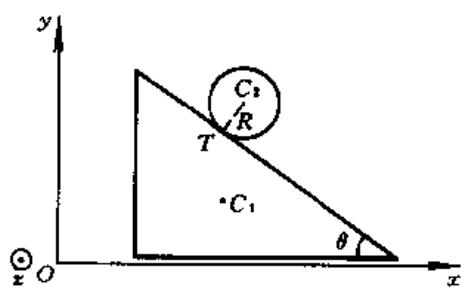
\includegraphics[width=0.25\textwidth]{figures/力图6-17-1.jpg}
\end{center}
\vfill
\newpage

\textbf{6-18} 如力图6-18-1，实心球在水平面内运动，质心的初始速度为 $\nu_{0}$ , 绕质心 $C$ 转动的初始角速度为 $\omega_{0}$ , 球与水平面之间的摩擦系数为 $\mu$ . 试分析球在水平面内的运动.

\begin{center}
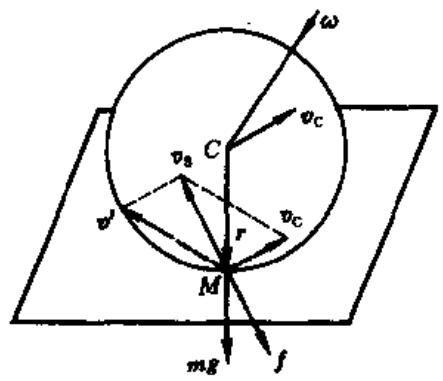
\includegraphics[width=0.2\textwidth]{figures/力图6-18-1.jpg}
\end{center}
\vfill


\textbf{6-19} 如力图6-19-1，一个质量为 $m$ , 半径为 $R_A$ 的均匀圆盘 $A$ 在光滑水平面 $Oxy$ 内以速度 $V$ 沿 $x$ 方向平动, 圆盘中心至 $x$ 轴的垂直距离为 $b$ . 圆盘 $A$ 与另一静止的、其中心位于坐标原点 $O$ 的均匀圆盘 $B$ 相碰. 圆盘 $B$ 的质量与 $A$ 相同, 半径为 $R_B$ . 假定碰撞后两圆盘接触处的切向速度分量相等, 并假定碰撞前、后两盘沿连心线方向的相对速度大小不变. 试求:

1. 碰后两圆盘质心速度的 $x$ 分量和 $y$ 分量 $V_{Ax}^{\prime}, V_{Ay}^{\prime}, V_{Bx}^{\prime}, V_{By}^{\prime}$ .

2. 碰后两圆盘的动能 $E_A'$ 和 $E_B'$ .

\begin{center}
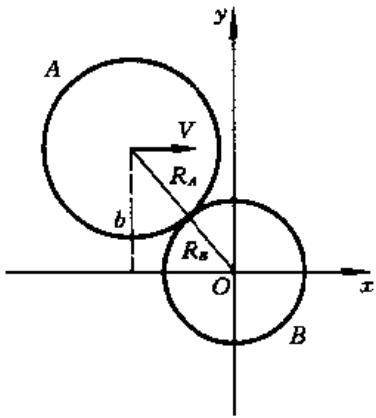
\includegraphics[width=0.2\textwidth]{figures/力图6-19-1.jpg}
\end{center}
\vfill
\newpage

\textbf{6-20} 如力图6-20-1，均匀细圆环半径为 $R$ ，质量为 $m$ ，平放在水平桌面上，与桌面之间的摩擦系数为 $\mu$ 。圆环质心 $O$ 沿 $x$ 轴以初速 $v_{\mathrm{C}0}$ 运动，同时圆环绕质心以初角速度 $\omega_0$ 顺时针转动， $v_{\mathrm{C}0}$ 与 $\omega_0$ 满足 $v_{\mathrm{C}0} = R\omega_0$ 。

试求: 1. 圆环所受摩擦力及摩擦力对质心的力矩. 2. 从开始到圆环停止运动所需时间.

\begin{center}
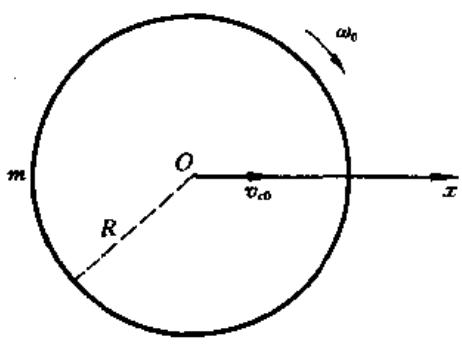
\includegraphics[width=0.25\textwidth]{figures/力图6-20-1.jpg}
\end{center}
\vfill


\textbf{6-21} 长为 $l$ 的均匀细杆竖直地放置在光滑地面上，从静止倒下．试求落到地面时的质心速度.
\vfill
\newpage


\textbf{6-22} 如力图6-22-1，光滑水平地面上静止地放着质量为 $M$ 、长为 $l$ 的均匀细杆。质量为 $m$ 的质点以垂直于杆的水平初速 $\upsilon_0$ 与杆的一端作完全弹性碰撞.

试求: 1. 碰后系统质心的速度及绕质心的角速度. 2. 实际的转轴(即静止点)位于何处.

\begin{center}
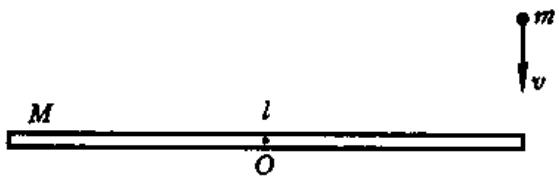
\includegraphics[width=0.3\textwidth]{figures/力图6-22-1.jpg}
\end{center}
\vfill


\textbf{6-23} 如力图6-23-1，长为 $2l$ 的均匀细杆，下端支在地面上，上端靠在竖直墙上，从静止下滑，开始时杆与地面的夹角为 $\theta_0$ 。设杆与地和墙之间的摩擦可略。试问质心下降到初始高度的几分之几时，杆的上端与墙脱离。

\begin{center}
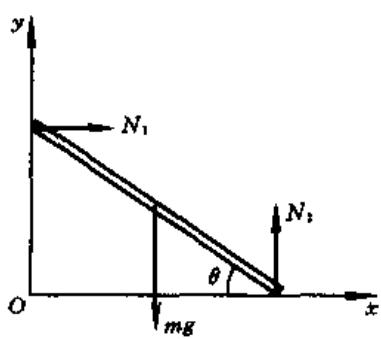
\includegraphics[width=0.25\textwidth]{figures/力图6-23-1.jpg}
\end{center}
\vfill
\newpage

\textbf{6-24} 如力图6-24-1，在光滑地面上静止地放置着两根质量均为 $m$ ，长度均为 $l$ 的均匀细杆.其中一杆由相等的两段构成，中间用光滑的铰链连接起来.在两杆的一端，各施以相同的垂直于杆的水平冲量 $J$ .试求两杆所获动能之比.

\begin{center}
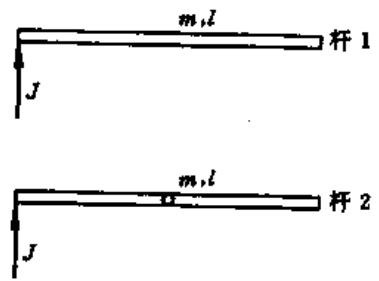
\includegraphics[width=0.25\textwidth]{figures/力图6-24-1.jpg}
\end{center}
\vfill


\textbf{6-25} 如力图6-25-1，半径为 $R$ 的圆环绕铅垂的直径轴以角速度 $\omega$ 匀角速旋转。一细杆长 $L = \sqrt{2} R$ , 其两端约束在圆环上可作无摩擦滑动, 细杆的位置用 $OC$ 与铅垂轴的夹角 $\theta$ 表示, $C$ 为细杆的质心。试求细杆在圆环上的平衡位置, 并讨论平衡的稳定性。

\begin{center}
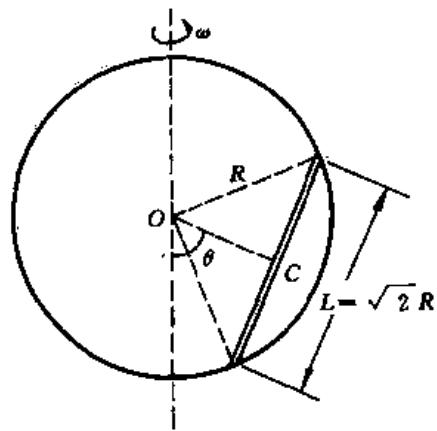
\includegraphics[width=0.2\textwidth]{figures/力图6-25-1.jpg}
\end{center}
\vfill
\newpage

\textbf{6-26} 如力图6-26-1， $Ox$ 和 $Oy$ 分别是支架的水平臂和铅垂臂， $Ox$ 臂绕铅垂臂作匀角速转动，角速度为 $\omega$ 。一均匀细杆的两端 $A$ 和 $B$ 被分别约束在两臂上运动，假定约束是理想的，细杆的质量为 $m$ ，长为 $2L$ ，细杆位置用图中 $\theta$ 角表示， $\theta$ 角是 $OC$ 与 $Oy$ 之间的夹角， $C$ 为细杆质心。以支架为参考系考察细杆的运动。

1. 试写出细杆的能量表达式。2. 试求细杆的平衡位置，并讨论平衡的稳定性。

\begin{center}
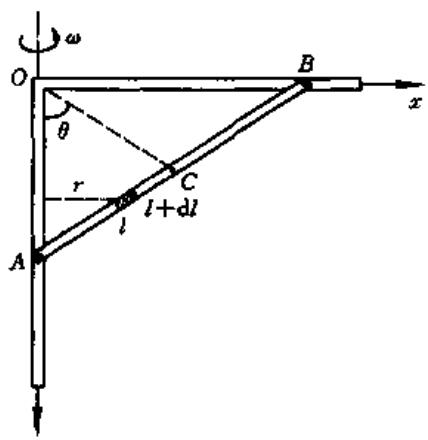
\includegraphics[width=0.2\textwidth]{figures/力图6-26-1.jpg}
\end{center}
\vfill


\textbf{6-27} 1. 如力图6-27-1，质量为 $m$ 的陀螺绕对称轴高速旋转, 角速度为 $\omega$ , 绕对称轴的转动惯量为 $I$ , 质心到转轴下端的距离为 $l_{\mathrm{C}}$ , 在重力矩的作用下, 陀螺将绕竖直轴作缓慢进动. 试求进动角速度的近似值.

2. 若转轴下端与桌面是面接触, 并受摩擦力的作用. 试解释在摩擦的作用下, 转轴将产生趋向于竖直轴的附加运动, 并计算从倾斜 $\theta$ 角到竖直位置所需的时间.

\begin{center}
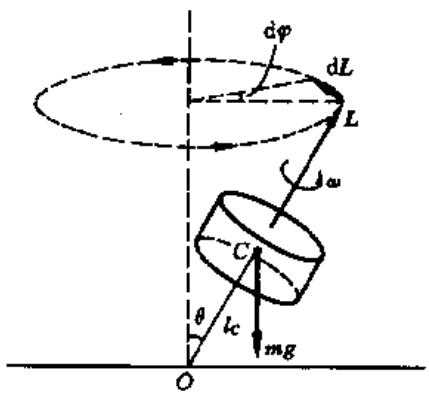
\includegraphics[width=0.25\textwidth]{figures/力图6-27-1.jpg}
\end{center}
\vfill




\chapter{振动与波动}
\newpage
\textbf{7-1} 【题1】如力图7-1-1，质量为 $m$ 、劲度系数为 $k$ 的弹簧振子放在光滑的水平面上，其平衡位置在 $O$ 点，其圆频率 $\omega = 0.5\pi \mathrm{rad}\cdot \mathrm{s}^{-1}$ 。另一质量亦为 $m$ 的质点放在光滑曲面的 $A$ 点， $AB$ 间高度差 $h = 0.20\mathrm{m}$ ，质点由 $A$ 点滑到 $B$ 点所需时间 $t_{AB} = 1.5\mathrm{s}, OB$ 之间的距离 $l = 6.0\mathrm{m}$ 。现将弹簧振子向左压缩到 $x_0 = 2.0\mathrm{m}$ 处自由释放，同时释放 $A$ 处的质点 $m$ ，两个质点相遇作完全非弹性碰撞后粘在一起，发生碰撞时弹簧作用力可略。若从碰撞开始计时，试求系统振动的数学表达式。（取 $g = 10\mathrm{m / s^2}$ ）。

\begin{center}
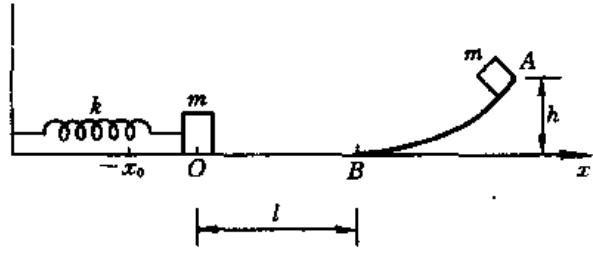
\includegraphics[width=0.3\textwidth]{figures/力图7-1-1.jpg}
\end{center}
\vfill

\textbf{7-2} 【题2】如力图7-2-1,某液体的密度随深度线性地增加,液体表面的密度为 $\rho_{0}$ , 深度为 D 处的密度为 $2\rho_{0}$ , 一密度为 $2\rho_{0}$ 的小球在深度为 $\frac{D}{2}$ 处从静止释放. 忽略液体的阻力. 试求小球的振动表达式.

\begin{center}
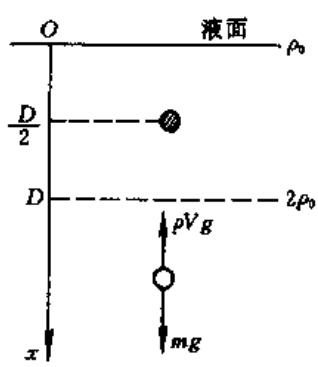
\includegraphics[width=0.2\textwidth]{figures/力图7-2-1.jpg}
\end{center}
\vfill

\newpage
\textbf{7-3} 【题3】如力图7-3-1,两个完全相同的圆柱状滚轮在水平面内平行放置,各绕自身的轴线按图示方向等角速转动,两轴线之间的距离为2l.在两滚轮上平放一块重量为G的均匀木板,木板与滚轮之间的摩擦系数为 $\mu$ .若木板重心偏离两轴中心位置一个微小的距离,试描述木板的运动.
\begin{center}
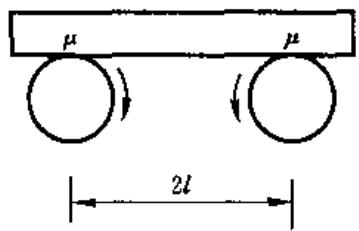
\includegraphics[width=0.25\textwidth]{figures/力图7-3-1.jpg}
\end{center}
\vfill

\textbf{7-4} 【题4】牛顿曾证明：一个均匀球壳，对球壳内物质的万有引力为零，而对球壳外物质的万有引

力不为零, 并且其作用就相当于球壳的质量都集中到球心那样(参看力学第三章题11). 如力图7-4-1所示, 设想沿地球直径开凿一条贯通地球的隧道, 将一小球从洞口由静止释放, 试求小球到达隧道另一洞口所用的时间. 已知地球的半径为 $R$ , 质量为 $M$ , 设地球的质量均匀分布.
\vfill

\newpage
\textbf{7-5} 【题5】如力图7-5-1，在倾角为 $\theta$ 的斜面上有一劲度系数为 $k$ 的弹簧，一端固定，另一端与质量为 $m$ 的实心圆柱体的轴连接，圆柱体在斜面上作纯滚动。忽略轴承的摩擦。试求振动周期。

\begin{center}
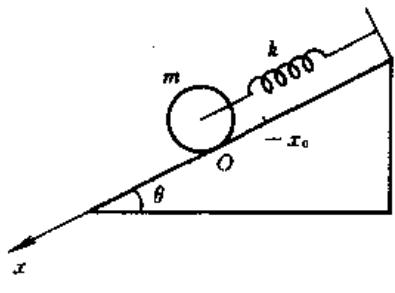
\includegraphics[width=0.2\textwidth]{figures/力图7-5-1.jpg}
\end{center}
\vfill

\textbf{7-6} 【题6】如力图7-6-1，直角形均匀细杆的水平杆长为 $l$ 、质量为 $m$ ，竖直杆长为 $2l$ 、质量为 $2m$ ，细杆可绕拐角处的固定轴 $\mathcal{O}$ 无摩擦地转动．水平杆的一端与劲度系数为 $k$ 的弹簧相连，平衡时水平杆呈水平状态,竖直杆竖直下垂.试求微小摆动的周期.

\begin{center}
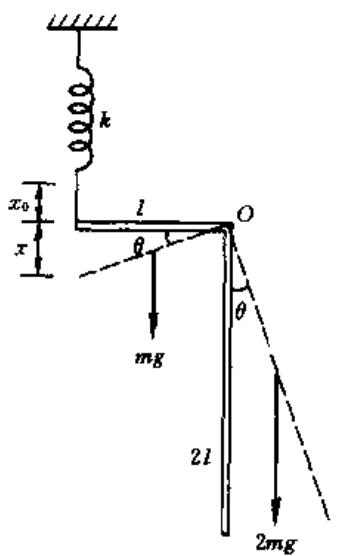
\includegraphics[width=0.2\textwidth]{figures/力图7-6-1.jpg}
\end{center}
\vfill

\newpage
\textbf{7-7} 【题7】如力图7-7-1, 弹簧振子中的小球质量为 $M$ , 弹簧的劲度系数为 $k$ , 弹簧的质量不可忽

略,设为 m, 假定弹簧的质量分布均匀, 忽略摩擦力. 试求振动周期.

\begin{center}
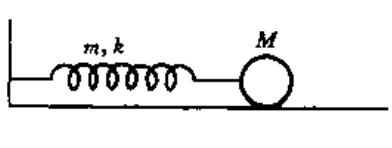
\includegraphics[width=0.3\textwidth]{figures/力图7-7-1.jpg}
\end{center}
\vfill

\textbf{7-8} 【题8】如力图7-8-1，一不可伸长的细线穿过光滑桌面上的小孔，一端系质量为 $m$ 的小球，另一端系质

量为 M 的重物．小球在桌面上以角速度 $\omega_{0}$ 作匀速圆周运动，重物静止不动．若重物受到竖直向上或向下的扰动．试证明，重物将作上、下的简谐振动，并求振动圆频率．

\begin{center}
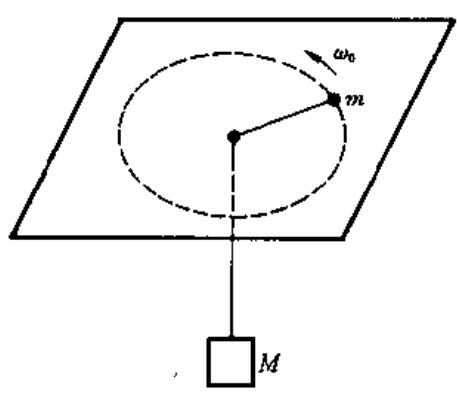
\includegraphics[width=0.25\textwidth]{figures/力图7-8-1.jpg}
\end{center}
\vfill

\newpage
\textbf{7-9} 【题9】如力图7-9-1，光滑的水平平板绕铅垂轴 $Oz$ 逆时针作匀角速转动，角速度为 $\omega$ 。在板面上，一质量可略、原长为 $l$ 、劲度系数为 $k$ 的弹簧一端固定在 $O$ 点，另一端系一质量为 $m$ 的小球。开始时小球位于 $(x_0,0)$ ，初速度为 $(v_0,0)$ 。试求小球相对平板的运动方程 $x = x(t), y = y(t)$ 。

\begin{center}
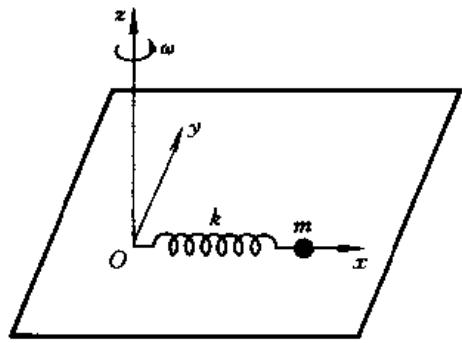
\includegraphics[width=0.2\textwidth]{figures/力图7-9-1.jpg}
\end{center}
\vfill

\textbf{7-10} 【题10】在有些湖中，有时可观察到一种奇妙的湖震现象（水振荡）。通常是在一个浅的，长而比较窄的湖里可以看到。好像水的整体在运动，像你拿着一杯咖啡送到客人那里去时那样。不能把这种现象当作湖面上的水波。

我们用一只矩形容器作模型．容器的长度为 L，水高为 h．假定水面开始时与水平面成一小角度．水面开始振荡，振荡时水面仍保持平面，只是绕位于容器长度一半处的水平轴作振荡．

1. 试建立水运动的模型, 并求出振荡周期 $T$ 的表达式. 初始条件在力图7-10-1中给出. 假定 $\xi \ll h$ .

2. 下面两个表显示在两种不同长度的容器中, 不同深度的水

的振荡时间．以适当的方法检查你得出的公式,看它是否与实验数据很好吻合,并说明你对这种物理模型的适用性的意见．

表 1 L = 479 mm

<table><tr><td>h/mm</td><td>T/s</td></tr><tr><td>30</td><td>1.78</td></tr><tr><td>50</td><td>1.40</td></tr><tr><td>69</td><td>1.18</td></tr><tr><td>88</td><td>1.08</td></tr><tr><td>107</td><td>1.00</td></tr><tr><td>124</td><td>0.91</td></tr><tr><td>142</td><td>0.82</td></tr></table>

表 2 L = 143 mm

<table><tr><td>h/mm</td><td>T/s</td></tr><tr><td>31</td><td>0.52</td></tr><tr><td>38</td><td>0.48</td></tr><tr><td>58</td><td>0.43</td></tr><tr><td>67</td><td>0.35</td></tr><tr><td>124</td><td>0.28</td></tr></table>

3. 力图 7-10-2 所示是在瑞典的 Vattern 湖上测量的结果, 两条曲线分别代表在湖的北端

Bastedalen 和南端 Jönköping 的测量．该湖长度为 123 km，平均深度为 50 m．在此情况下，时间标度应是什么？

\begin{center}
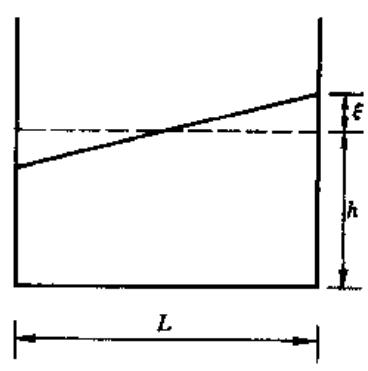
\includegraphics[width=0.3\textwidth]{figures/力图7-10-1.jpg}
\end{center}
\vfill

\newpage
\textbf{7-11} 【题11】如力图7-11-1，质量为 $m_{1}$ 的滑块可在光滑水平直导轨上滑动，滑块经长为 $l$ 质量可略的细杆

与质量为 $m_{2}$ 的重锤相连，细杆与重锤可绕滑块无摩擦地自由转动。设 $t = 0$ 时，细杆与导轨构成铅垂面，细杆与铅锤线夹角 $\theta_0$ ，从静止释放开始摆动。试求：1. 重锤 $m_{2}$ 的运动轨迹。2. 系统作小角摆动时，滑块位置随时间的变化。

\begin{center}
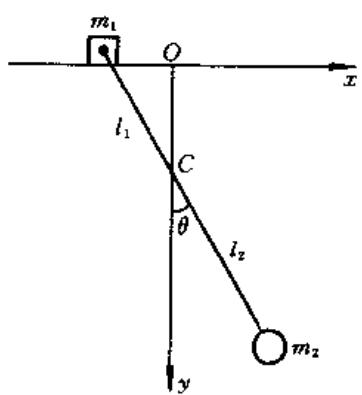
\includegraphics[width=0.2\textwidth]{figures/力图7-11-1.jpg}
\end{center}
\vfill

\textbf{7-12} 【题12】如力图7-12-1,质量为 $m$ , 半径为 $r$ 的均匀实心小球在半径为 $R$ 的球形碗底作纯滚动. 试求微小振动的周期.

\begin{center}
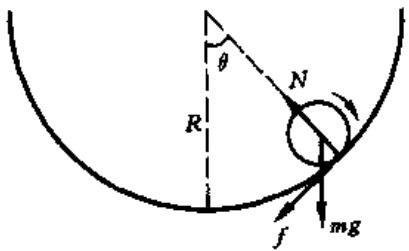
\includegraphics[width=0.2\textwidth]{figures/力图7-12-1.jpg}
\end{center}
\vfill

\newpage
\textbf{7-13} 【题13】如力图7-13-1, 质量为 $M$ 的物体放置在两个完全相同的质量均为 $m$ 的薄壁中空圆筒上. 物体两侧系着两个完全相同的劲度系数均为 $k$ 的弹簧, 两弹簧的另一端固定, 开始时两弹簧均为原长. 设物体在两薄圆筒上作纯滚动. 试求振动圆频率.

\begin{center}
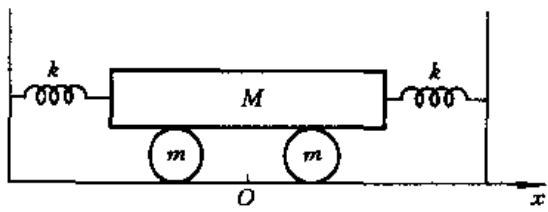
\includegraphics[width=0.3\textwidth]{figures/力图7-13-1.jpg}
\end{center}
\vfill

\textbf{7-14} 【题14】如力图7-14-1，圆盘绕通过中心 $O$ 点的竖直轴在水平面内匀速转动，角速度为 $\omega$ ，质量为 $m$ 的小球被约束在圆盘上的光滑导轨 $AB$ 内运动。小球与一劲度系数为 $k$ 的弹簧相连 $(k > m\omega^2)$ ，弹簧另一端固定在圆盘 $A$ 点。弹簧为原长时，小球位于 $P$ 点， $OP = r_0$ ，且 $OP \perp AB$ ，将小球从 $P$ 点沿导轨拉开距离 $a$ 后从静止释放。在圆盘参考系中考察小球的运动。

1. 试求小球的平衡位置.2. 试证明小球作简谐振动,并求圆频率.3. 试求导轨施予小球的水平力随时间的变化规律.4. 试问当 $k < m\omega^2$ 时小球怎样运动.

\begin{center}
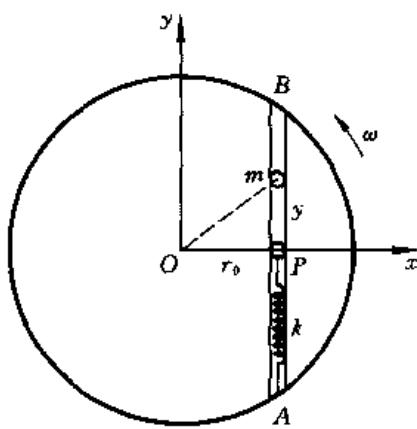
\includegraphics[width=0.2\textwidth]{figures/力图7-14-1.jpg}
\end{center}
\vfill

\newpage
\textbf{7-15} 【题15】如力图7-15-1，质量为 $m$ 的小球在光滑水平桌面上以角速度 $\omega$ 作匀速圆周运动。所需的向心力由与小球相连的弹簧提供，弹簧的劲度系数为 $k$ ，另一端固定。今沿径向轻击小球。试求小球径向振动的频率。

\begin{center}
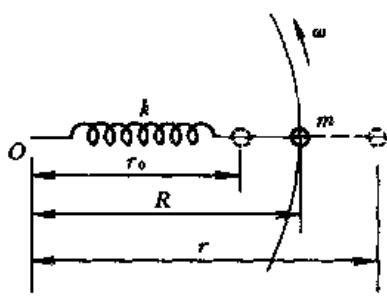
\includegraphics[width=0.2\textwidth]{figures/力图7-15-1.jpg}
\end{center}
\vfill

\textbf{7-16} 【题16】计算单摆周期时，若摆幅 $\theta_0$ 较小，可采用一级近似 $\sin \theta \approx \theta$ ，算出的周期为 $T_{0} = 2\pi \sqrt{\frac{l}{g}}$ ，其中 $l$ 为摆长。若 $\theta_0$ 不算小，就应取二级近似。试导出单摆周期 $T$ 与摆幅 $\theta_0$ 的关系。
\vfill

\newpage
\textbf{7-17} 【题17】对于谐振子, 若广义动量为 $p$ , 广义坐标为 $q$ , 则有 $\oint p \mathrm{d} q = \frac{E}{\nu}$ , 其中 $E$ 为谐振子的能量, $\nu$ 为振动频率. 积分在振动的一个周期内进行. 试就弹簧振子和单摆的情况证明此式.
\vfill

\textbf{7-18} 【题18】如力图7-18-1, $T$ 形导轨固定在铅垂面内, 质量为 $m$ 、全长为 $l$ 的刚性均匀细杆两端约束在 $T$ 形导轨中, 可沿导轨作无摩擦的滑动. 1. 试求细杆作小振幅摆动时的振动周期. 2. 当细杆摆至右方适当角度刚好达到静止时 (如力图7-18-1中虚线所示), 一质量也为 $m$ 的小球以速度 $v_{0}$ 沿水平方向经导轨与细杆上端相碰. 设碰撞无机械能损失, 碰后小球速度变为零, 细杆则回摆到左方与水平导轨平行时刚好静止. 试问 $v_{0}$ 应为多大?

\begin{center}
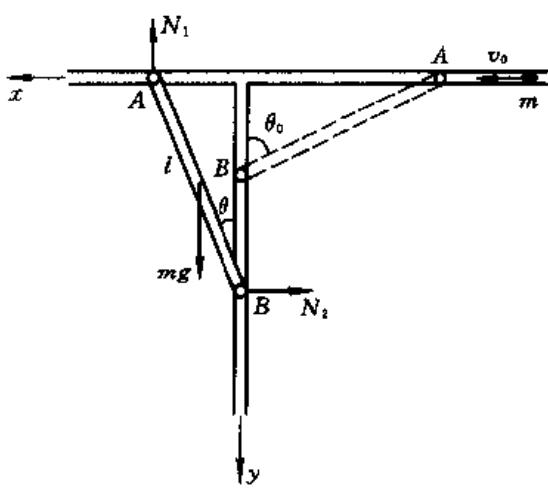
\includegraphics[width=0.25\textwidth]{figures/力图7-18-1.jpg}
\end{center}
\vfill

\newpage
\textbf{7-19} 【题19】如力图7-19-1，在光滑水平面上，质量为 $m_{1}$ 和 $m_{2}$ 的两物体用劲度系数为 $k$ 的弹簧相连。当弹簧为原长时， $m_{1}$ 与 $m_{2}$ 相距 $l_{0}$ ，把弹簧压缩距离 $a$ 后从静止释放。试求 $m_{1}$ 和 $m_{2}$ 的振动表达式。

\begin{center}
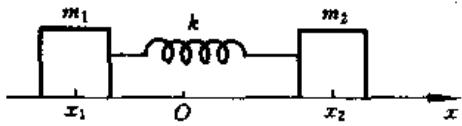
\includegraphics[width=0.3\textwidth]{figures/力图7-19-1.jpg}
\end{center}
\vfill

\textbf{7-20} 【题20】如力图7-20-1，单摆的原长为 $l_{0}$ ，在摆动过程中缓慢上拉，悬点位置不变而摆长逐渐缩短。试求

当摆长缩短为原长之半，即 $l = \frac{l_0}{2}$ 时的振幅与原振幅之比。

\begin{center}
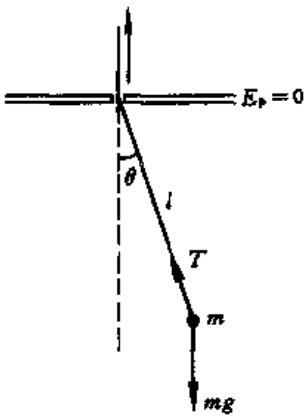
\includegraphics[width=0.2\textwidth]{figures/力图7-20-1.jpg}
\end{center}
\vfill

\newpage
\textbf{7-21} 【题21】如力图7-21-1，质量为 $M$ 、长为 $L$ 的均匀刚性细杆的一端悬挂，可在铅垂面内绕悬点无摩擦地

摆动．质量为 $m=\frac{M}{3}$ 的小虫相对杆以速度 $v_{s}$ 缓慢地沿杆向下爬行．开始时，杆静止并与竖直线夹 $\theta_{0}$ 角（设 $\theta_{0}$ 很小）；小虫位于杆上端的悬点．放开后，杆开始摆动，小虫开始爬行．

试求:1. 小虫沿杆爬行 l 距离时,杆摆动的圆频率.2. 小虫爬到杆下端时,杆摆动的幅度.

\begin{center}
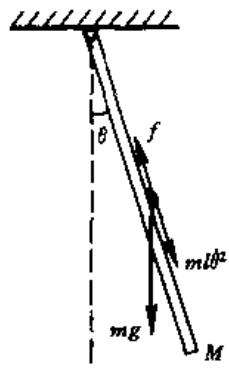
\includegraphics[width=0.15\textwidth]{figures/力图7-21-1.jpg}
\end{center}
\vfill

\textbf{7-22} 【题22】如力图7-22-1，圆盘在水平面内以匀角速 $\Omega$ 绕竖直轴 $OO'$ 旋转，盘上固连着两根同样高度的竖直支架。质量为 $m$ 的小球与质量可忽略不计的 $T$ 字形细杆相连，水平杆由支架支承，与小球相连的杆长为 $l$ ，悬点 $O'$ 在转轴上，整个系统可在支架上无摩擦地摆动。

试求:1. 小球的平衡位置.2. 小球作小幅摆动时的圆频率.

\begin{center}
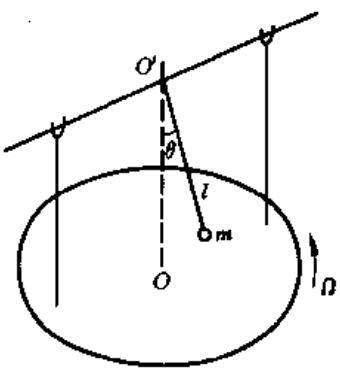
\includegraphics[width=0.2\textwidth]{figures/力图7-22-1.jpg}
\end{center}
\vfill

\newpage
\textbf{7-23} 【题23】如力图7-23-1，在光滑水平面上有三质点 $A, B, C$ ，质量分别为 $m_1, m_2$ 和 $m_3$ ，三质点位于同一直线上，开始时 $B$ 和 $C$ 静止，用劲度系数为 $k$ 的弹簧（质量忽略）相连。质点 $A$ 以初速 $v_0$ 沿连线方向与 $B$ 作完全弹性碰撞。



1. 以 $A$ 和 $B$ 的碰撞点为坐标原点, 连线为 $x$ 轴, 试求碰后质点 $B$ 的运动规律. 2. 设 $m_2 = m_3 = m$ , 为使质点 $A$ 和 $B$ 在碰后重新相遇, 但不相碰 (即相遇时速度相同), 试问比值 $\frac{m_1}{m}$ 应为多少?

\begin{center}
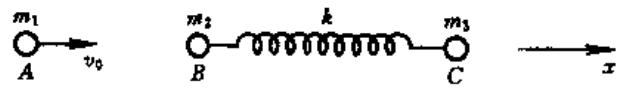
\includegraphics[width=0.35\textwidth]{figures/力图7-23-1.jpg}
\end{center}
\vfill

\textbf{7-25} 【题25】如力图7-25-1，质量为 $m$ 、长为 $l$ 的均匀长方形木板由劲度系数分别为 $k_{1}$ 和 $k_{2}$ 的两竖直弹簧在两端支撑，平衡时木板位于水平面。试求木板作小幅振动时的特征频率。

\begin{center}
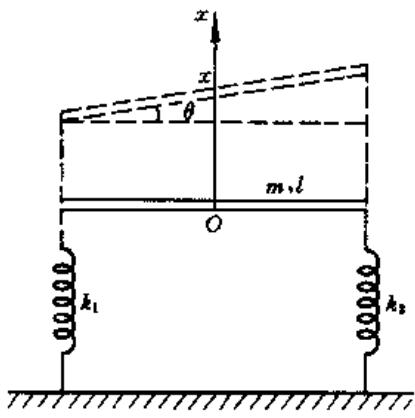
\includegraphics[width=0.25\textwidth]{figures/力图7-25-1.jpg}
\end{center}
\vfill

\newpage
\textbf{7-26} 【题26】如力图7-26-1,两个完全相同的单摆并排悬挂,摆球质量均为 $m$ ,摆长均为 $l$ ,两摆球用劲度系数为 $k$ 的轻质弹簧连接,弹簧原长等于两悬点之间的距离.忽略空气阻力.上述振

动系统称为耦合摆．在小角摆动的条件下，1. 试求耦合摆的特征频率，并写出两摆球运动方程的一般表达式．2. 试讨论耦合摆在不同初始条件下的几种典型运动情况．

\begin{center}
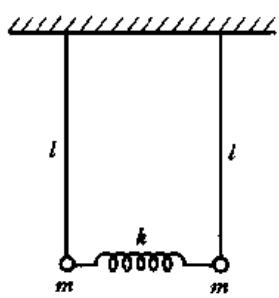
\includegraphics[width=0.2\textwidth]{figures/力图7-26-1.jpg}
\end{center}
\vfill

\textbf{7-27} 【题27】如力图7-27-1，6个质量均为 $m$ 的小球串在光滑圆环上，彼此间用劲度系数均为 $k$ 的6个弹簧相连，整个系统在水平面内。当各小球处在平衡位置时，弹簧均为原长。试求特征频率。

\begin{center}
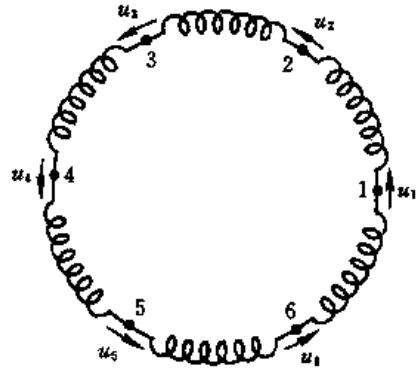
\includegraphics[width=0.2\textwidth]{figures/力图7-27-1.jpg}
\end{center}
\vfill

\newpage
\textbf{7-28} 【题28】三个质量各为 $m$ 的质点由未伸长的无质量弹簧连接在一起达到平衡。每个弹簧的劲度系数为 $k$ ，它们被限制在圆周上运动，如力图7-28-1所示。

1. 若每一质点 $m$ 分别有偏离平衡位置的小位移 $u_{1}, u_{2}$ 和 $u_{3}$ , 试写出每一质点的运动方程

2. 试验证此系统有下列简谐式解
$$
u _ {n} = a _ {n} \cos \omega t
$$
其加速度为 $-\omega^2 u_n$ ，此处 $a_n (n = 1,2,3)$ 是恒振幅，角频率 $\omega$ 有下列三个可能的取值，即
$$
\sqrt {3} \omega_ {0}, \sqrt {3} \omega_ {0}, 0
$$
其中 $\omega_{0}^{2}=\frac{k}{m}$ .

3. 将这由弹簧与质点交替连接的系统扩充到 N 个质点，每一质点 m 由弹簧与相邻质点连接。起初弹簧未伸长，处于平衡，当质点偏离平衡时，用第 n 个质点的位移和相邻质点的位移表示出第 n 个质点 $(n=1,2,\cdots,N)$ 的运动方程。试验证
$$
u _ {n} (t) = a _ {s} \sin \left(\frac {2 n s \pi}{N} + \varphi\right) \cos \omega_ {s} t
$$
是振荡解，式中 $s=1,2,\cdots,N,n=1,2,\cdots,N,\varphi$ 为一任意相位，角频率 $\omega_{s}$ 由下式给出
$$
\omega_ {s} = 2 \omega_ {0} \sin \left(\frac {s \pi}{N}\right)
$$
而 $a_{s}(s=1,2,\cdots,N)$ 是与 n 无关的恒振幅。

试叙述对于一个含有无穷多个质点的链条,频率的可能范围.

4. 试确定 $\frac{u_n}{u_{n+1}}$ 的比值。

当 $N$ 很大时, 对于下列 $(a), (b)$ 两种情况, 试画出说明时刻 $t$ 质点的位移与该质点在链上编号之间关系的草图.

(a)低频解.

$(b)\omega_{s}=\omega_{\max}$ ，其中 $\omega_{\max}$ 是最大的频率解。

5. 若质点之一用质量 $m^{\prime} \ll m$ 的质点代替, 试估计角频率分布将发生怎样的主要变化.

试在上面结果的基础上定性地描述,由质量为 m 和 $m'$ 交替联接的双原子链会有怎样形式的频谱.

提示：
$$
\begin{array}{r l} \sin (A + B) & = \sin A \cos B + \cos A \sin B \\ \sin A + \sin B & = 2 \sin \frac {A + B}{2} \cos \frac {A - B}{2} \\ 2 \sin^ {2} A & = 1 - \cos 2 A \end{array}
$$

\begin{center}
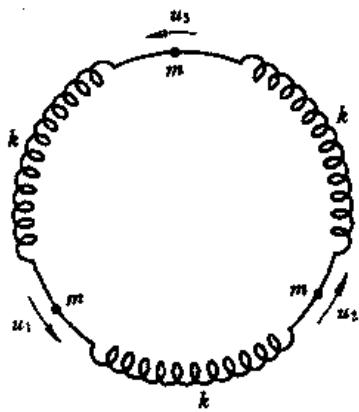
\includegraphics[width=0.2\textwidth]{figures/力图7-28-1.jpg}
\end{center}
\vfill
\newpage

\textbf{7-29} 【题29】如力图7-29-1，细杆长 $l$ ，上端 $O$ 悬挂，下端与质量为 $m$ 的摆球相连，摆球可绕 $O$ 轴无摩擦地摆动。今在细杆的 $A$ 点经连杆接一阻尼器，阻尼力 $f$ 沿水平方向，其大小

与阻尼板的速度 $v$ 成正比，即 $f = \gamma v, \gamma$ 为阻力系数。设 $OA = a$ ，细杆、连杆、阻尼板等的质量均远小于 $m$ ，可忽略不计，阻尼较弱。试求小幅阻尼振动的对数减缩，以及一周期内损失能量的百分比。

\begin{center}
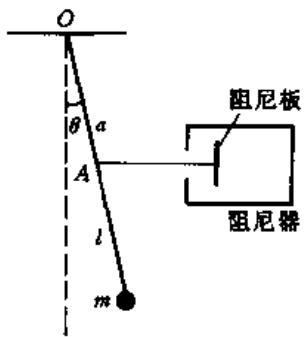
\includegraphics[width=0.2\textwidth]{figures/力图7-29-1.jpg}
\end{center}
\vfill


\textbf{7-30} 【题30】质量为 $m$ 的质点在弹性力和阻尼力的作用下沿 $x$ 轴运动。取平衡位置为坐标原点，弹性力为 $-kx$ ，阻尼力为 $-\gamma x$ 。试问，是否在临界阻尼情况下，质点回到平衡位置一定最快？
\vfill
\newpage


\textbf{7-31} 【题31】如力图7-31-1，充满液体的容器在竖直方向上下振动，质量为 $m$ 的重物由劲度系数为 $k$ 的弹簧悬挂，浸没在液体之中。设悬点随容器振动的规律为 $x_{H} = A\cos \omega t$ ，设液体的阻尼系数为 $\gamma$ （弱阻尼），并假定液体的浮力恒定。

1. 若 $\omega = \omega_0$ ，试求稳定后重物的振动表达式，其中 $\omega_0 = \sqrt{\frac{k}{m}}$ 为弹簧振子的固有圆频率。

2. 若 $\omega \gg \omega_0$ ，试求稳定后重物的振动表达式。

3. 若 $\omega \gg \omega_{0}$ ，且当容器达到最高点时突然停止不动，试求此后重物的振动表达式。

4. 试画出容器突然停止以前和以后的振动曲线。

\begin{center}
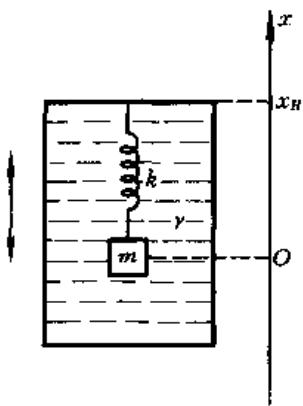
\includegraphics[width=0.2\textwidth]{figures/力图7-31-1.jpg}
\end{center}
\vfill


\textbf{7-32} 【题32】如力图7-32-1，质量均为 $m$ 的三个滑块放置在光滑水平桌面上，彼此以原长为 $x_0$ 、劲度系数为

k 的二个相同弹簧连接起来。开始时三滑块静止，滑块 A 位于原点 O，两弹簧均为原长。对滑块 A 施以周期性外力 F，已知 $F = F_{0} \cos \omega t$ ，在水平方向并沿三滑块连线。试求振动系统的特征频率，并写出滑块 C 的运动方程。

\begin{center}
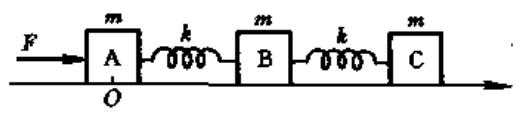
\includegraphics[width=0.3\textwidth]{figures/力图7-32-1.jpg}
\end{center}
\vfill
\newpage

\textbf{7-33} 【题33】本世纪初曾提出一种地球模型，认为它是一个半径为 $R$ 的球体，从地球表面向内到半

径 $R_{C}$ 处为均匀各向同性的固态地幔， $R_{C}$ 以内的地芯为液态，如力图 7-33-1 所示。

在地幔内,地震纵波 p 和横波 s 的速度分别为常量 $v_{p}$ 和 $v_{s}$ ; 在地芯内,纵波的速度为常量 $v_{Cp}$ , 且 $v_{Cp} < v_{p}$ , 而横波不传播.

在地球表面 E 处发生了一次地震, 产生的地震波在地球内传播, 且被地球表面 X 处设置有地震仪的观察者观察到 .E 点和 X 点的角间隔 $2\theta = \angle EOX$ , 其中 O 为地球中心.

1. 试证明, 对于 $\theta \leqslant \arccos \frac{R_C}{R}$ 的那些 $X$ 点, 从 $E$ 点发出的地震波沿直线穿过地幔传播到 $X$ 点的时间为 $t = \frac{2R\sin\theta}{v}$ , 对于 $p$ 波, $v = v_p$ , 对于 $s$ 波 $v = v_s$ .

2. 对于 $\theta > \arccos \frac{R_C}{R}$ 的那些 $X$ 点，地震 $p$ 波在地幔和地芯的界面上经过两次折射后到达 $X$ 点。画出这种地震 $p$ 波的传播路径，并求出对于 $p$ 波， $\theta$ 和 $i$ 之间的关系式，这里 $i$ 是 $p$ 波在地幔和地芯界面上的入射角。

3. 利用下列数据和第2问中所得结果，画出 $\theta \sim i$ 图形. $R = 6370\mathrm{km}, R_C = 3470\mathrm{km}, v_p = 10.85\mathrm{km/s}, v_s = 6.31\mathrm{km/s}, v_{Cp} = 9.02\mathrm{km/s}$ . 试评论，对于地球表面不同地点的观察者，从上述 $\theta \sim i$ 图形可得出什么物理结论.

4. 在一次地震后, 某观察者测出 $s$ 波相对 $p$ 波的时间延迟为 2 分 11 秒, 试用第 3 问中给出的数据确定地震地点与观察者之间的角间隔.

5. 在上述测量中, 观察者注意到某次 $p$ 波和 $s$ 波到达后, 地震仪上还有两个相间 6 分 37 秒的记录. 试解释这一结果, 并验证这与第 4 问所得的角间隔确实相符.
\vfill
\newpage


\textbf{7-34} 【题34】到晚上,地面辐射降温使空气层产生温度梯度,温度随高度递增,这导致声速 $v$ 随高度 $y$ 变化.假定变化规律为

$$
v = v _ {0} (1 + a ^ {2} y ^ {2})
$$

式中 $v_{0}$ 是地面 $(y = 0)$ 处的声速， $\alpha$ 为比例系数。今远方地面上某声源发出一束声波，发射方向与竖直方向成 $\theta_{0}$ 角。假定在声波传播范围内 $\alpha y \ll 1$ 。试导出该束声波在空间传播所循的轨迹，并求地面上听得最清晰的地点与声源的距离。
\vfill
\newpage

\textbf{7-35} 【题35】在海洋中，声波的速度随深度、温度和含盐量变化。已知声速随深度变化的规律如力图7-35-1所示。最小声速 $v_{0}$ 出现在海洋表面和海底之间，以最小声速处作为坐标原点， $z_{s}$ 和 $z_{b}$ 分别表示海洋表面和海底的坐标，则声速v与z的关系为

$$
v = \left\{ \begin{array}{l l} v _ {0} + b z & (z > 0) \\ v _ {0} & (z = 0) \\ v _ {0} - b z & (z <   0) \end{array} \right.
$$

其中 $b$ 为正的常量.

如力图7-35-2，今在 $x = 0, z = 0$ 处放置一声源 $S$ 。在 $zx$ 平面内，从 $S$ 发出的声波的传播方向用初始发射角 $\theta_0$ 表示。声速的不均匀将导致波射线的弯曲。

1. 试证明在 $zx$ 平面内声波的初始轨迹是半径为 $R$ 的圆弧，且

$$
R = \frac {v _ {0}}{b \sin \theta_ {0}} \quad \left(0 \leqslant \theta_ {0} <   \frac {\pi}{2}\right)
$$

2. 在不被海洋表面反射的声波中, 最小的 $\theta_{0}$ 是什么?

3. 设在 Ox 轴上 x = X 处设置接收器 H，试导出能直接到达接收器的各声波所对应的 $\theta_{0}$ 的公式。（排除经海洋表面和海底而到达接收器的情形。）

4. 已知 $X = 10000 \mathrm{~m}, v_0 = 1500 \mathrm{~m/s}, b = 0.020 \mathrm{~s}^{-1}$ . 试用这些数据计算可使声波直接从 $S$ 传到 $H$ (不经反射) 的 4 个 $\theta_0$ 的值 (从最小的 $\theta_0$ 开始).

5. 当 $\theta_0$ 取第3问中得出的最小值时, 试导出声波从 $S$ 传播到 $H$ 所需时间的表达式, 并用第4问所给的数据算出这个传播时间. 再计算当 $\theta_0 = \frac{\pi}{2}$ 时, 即声波沿 $x$ 传播到 $H$ 所需的时间. 比较上述两个时间的大小.

\begin{center}
    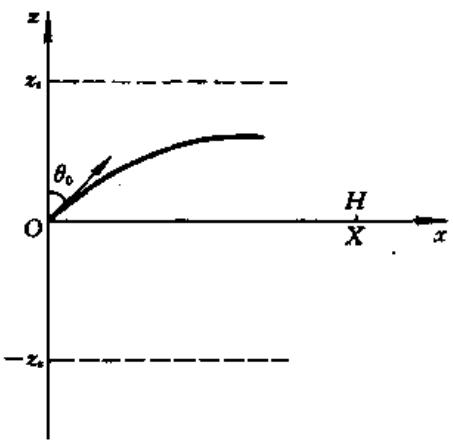
\includegraphics[width=0.2\textwidth]{figures/力图7-35-2.jpg}
    \quad
    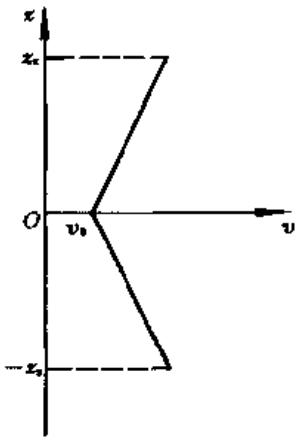
\includegraphics[width=0.15\textwidth]{figures/力图7-35-1.jpg}
\end{center}

\vfill

\newpage


\textbf{7-36} 【题36】如力图7-36-1,质量为 $m$ 、劲度系数为 $\pmb{k}$ 的弹簧原长为 $L$ ,一端固定,另一端与一质量为 $M$ 的物体相连,整个系统水平放置,物体 $M$ 可在光滑水平面上滑动.1.试导出纵向弹性波的波动方程并求波速.2.假定 $L$ 远小于弹性波的波长, $M$ 的振幅为 $A_0$ ,试求弹簧上各点的振幅分布.3.在 $m \ll M$ 的条件下,试分别求零级近似和一级近似的频率.

\begin{center}
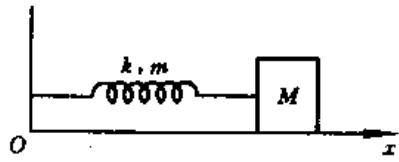
\includegraphics[width=0.3\textwidth]{figures/力图7-36-1.jpg}
\end{center}
\vfill

\textbf{7-37} 【题37】无穷长弦线，拉紧，质量线密度为 $\rho = 0.01\mathrm{kg / m}$ 。今在线一端施以横向简谐力，峰值为 $F_{\max} = 0.3\mathrm{N}$ ，使弦线中产生简谐振动，波速为 $v = \frac{30}{\pi}\mathrm{m / s}$ 。试求单位时间内通过弦线某一截面传输的平均能量 $S$ 。
\vfill

\newpage
\textbf{7-38} 【题38】拉紧的弦线，张力为 $T$ ，质量线密度为 $\rho$ ，质量为 $m$ 的质点附在弦上某点．圆频率为 $\omega$ 的波沿弦线传播．试求波在质点 $m$ 反射时的能量反射系数．
\vfill

\textbf{7-39} 【题39】音叉与频率为 $250.0\mathrm{Hz}$ 的标准声源同时发音时，产生 $1.5\mathrm{Hz}$ 的拍音。当音叉粘上一小块橡皮泥时，拍频增加了。如力图7-39-1，将该音叉放在盛水的细管口，连续调节水面的高度，当空气柱高度相继为 $0.34\mathrm{m}$ 和 $1.03\mathrm{m}$ 时发生共振。

试求:

1. 声波在空气中的声速.

2. 画出空气柱中的驻波图.

\begin{center}
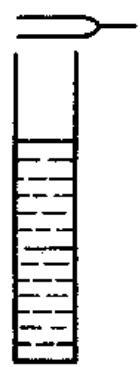
\includegraphics[width=0.1\textwidth]{figures/力图7-39-1.jpg}
\end{center}
\vfill

\newpage
\textbf{7-40} 【题40】小提琴弦长为 $L$ ，质量线密度为 $\rho$ ，张力为 $T.1$ 。用手指轻按弦的中点，试求基频和一次谐波的频率，并写出弦上各点的振动方程式。2. 在弦的一端 $\frac{L}{3}$ 长度上均匀包缠细线，使其线密度增加为 $4\rho$ ，放开手指，试求基频，并写出弦上各点的振动表达式。
\vfill\newpage

\textbf{7-41} 【题41】一列振幅为 $A$ ，频率为 $\nu$ ，波长为 $\lambda$ 的横波沿一拉紧的水平细线传播。细线单位长度的质量为 $\rho$ 。任一点位移的表达式为
$$
y _ {1} = A \sin 2 \pi \left(\nu t - \frac {x}{\lambda}\right)
$$

式中 $t$ 为时间, $x$ 为细线上各点的水平坐标.

另一列具有相同振幅、频率、波长的波同时在细线中沿相反方向传播。两列波 $t = 0$ 时在 $x = 0$ 处的相位差为 $\varphi$ 。今在 $x = 0$ 和 $x = L$ 两处将细线固定。

1. 试导出细线中的驻波方程，并求细线中所有可能存在的波长。

2. 试求任意时刻的总动能和总势能，规定细线上各点均处于平衡位置时的总势能为零点。

3. 设 $L = 2.50 \mathrm{~m}$ , 长为 $L$ 的细线的质量为 $m = 0.0100 \mathrm{~kg}$ , 细线中的张力 $T = 10.0 \mathrm{~N}$ , 驻波的最大振幅为 $0.02 \mathrm{~m}$ . 

(a) 试求基模的频率和对应的总能量. 

(b) 用手拨动细线, 在其中激起所有可能的驻波模式, 然后在距端点 $0.50 \mathrm{~m}$ 处抓住细线. 试问哪些频率的驻波可在细线中继续存留.



\vfill
\newpage



\textbf{7-42}  【题42】飞机在上空以速度 $v = 200\mathrm{m / s}$ 作水平飞行，发出频率为 $\nu_{0} = 2000\mathrm{Hz}$ 的声波。静止在地面上的观察者测定飞机发出的声波的频率，当飞机越过观察者上空时，观察者在 $4\mathrm{s}$ 钟内测出的频率从 $\nu_{1} = 2400\mathrm{Hz}$ 降为 $\nu_{2} = 1600\mathrm{Hz}$ 。已知声波在空气中的速度为 $v = 330\mathrm{m / s}$ ，试求飞机的飞行高度 $h$ 。

\vfill





\textbf{7-43}  【题43】如图，音叉 $P$ 沿着半径 $r = 8\mathrm{m}$ 的圆以角速度 $\omega = 4\mathrm{rad / s}$ 作匀速圆周运动。音叉发出频率为 $\nu_{0} = 500\mathrm{Hz}$ 的声波，声波的速度为 $v = 330\mathrm{m / s}$ 。观测者 $M$ 与圆周共面，与圆心 $O$ 的距离为 $d = 2r$ 。试问当 $\theta$ 角为多大时，观测到的频率为最高或最低，并求其数值。 $\theta$ 是 $OP$ 和 $OM$ 的夹角。

\begin{center}
    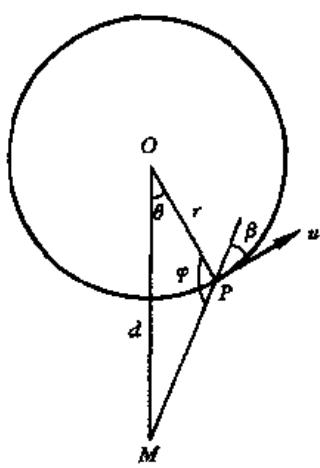
\includegraphics[width = 0.2\textwidth]{figures/力图7-43-1.jpg}
\end{center}

\vfill





% ========== 第二部分 热学 ==========


\chapter{平衡态理想气体}
\newpage
\textbf{1-1} 【题1】道尔顿提出过一种定压温标。在此温标下，压强为一恒定值时，理想气体体积的相对增量正比于温度 $\tau$ 的增量，且也将冰点定为 $\tau = 0^{\circ}$ ，汽点定为 $\tau = 100^{\circ}$ 。试用摄氏温度 $t$ 来表示道尔顿温度 $\tau$ 。
\vfill

\textbf{1-2} 【题2】某热电偶测温计的一个触点始终保持为 $0^{\circ}\mathrm{C}$ ，另一触点与待测温度的物体接触。当待测温度为 $t^{\circ}\mathrm{C}$ 时，测温计中的热电动势为
$$
\mathcal {E} = \alpha t + \beta t ^ {2}
$$
其中 $\alpha = 0.20\mathrm{mV} / \mathrm{C},\beta = -5.0\times 10^{-4}\mathrm{mV} / (\mathrm{C})^2.$

如果以热电偶的热电动热 $\varepsilon$ 为测温属性，规定下述线性关系来定义温标 $t^{*}$ ：
$$
t ^ {*} = a \mathcal {E} + b
$$

并规定冰点的 $t^* = 0^\circ$ ，汽点的 $t^* = 100^\circ$ .试画出 $t^{*}(t)$ 曲线.
\vfill

\newpage
\textbf{1-3} 【题3】贮气罐的体积为 $V$ ，罐内气体压强为 $p$ 。贮气罐经阀门与体积为 $V_0$ 的真空室相连，打开阀门，为真空室充气，达到平衡后，关闭阀门；然后换一个新的同样的贮气罐继续为真空室（已非“真空”）充气；…。如此不断充气，直到真空室中气体的压强达到 $p_0 (p_0 < p)$ 为止。设充气过程中温度恒定不变。试问共需多少个贮气罐。
\vfill

\textbf{1-4} 【题4】如热图1-4-1，在地面上竖直放置一个截面均匀的 $U$ 型管，管内盛有水。如热图1-4-1所示，管的右上端开口，左上端封口，左侧水面与上端相距 $h_1 = 30\mathrm{cm}$ ，其间封有一定质量的理想气体，右侧水面与上端相距 $h_2 = 20\mathrm{cm}$ 。在右侧水面上放置一个质量可忽略不计的薄活塞，它与管壁间既无空隙又无摩擦。当从右侧上端缓慢注入高为 $H = 7.5\mathrm{cm}$ 的水银柱时，发现水银柱的上表面恰好与左侧水面等高。设注入水银过程中，环境温度与空气压强均不变。已知水银密度是水密度的13.6倍。试求空气压强 $p_0$ 的大小
\begin{center}
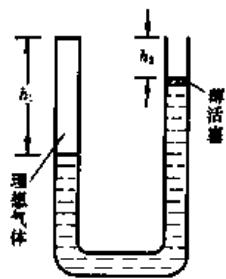
\includegraphics[width=0.2\textwidth]{figures/热图1-4-1.jpg}
\end{center}
\vfill

\newpage
\textbf{1-5} 【题5】在一端封闭、一端开口、内径均匀的直玻璃管内，有一段 $60\mathrm{mm}$ 长的水银柱。当管水平

放置达到平衡时, 闭端 A 管内空气柱长 140 mm, 开端 B 管内空气柱长也为 140 mm, 如热图 1-5-1 所示. 今将此管轻轻倒转, 使开口向下, 然后再竖直地插入水银槽内, 达到平衡时管中闭端 A 管内空气柱长 133 mm, 设大气压强为 760 mmHg, 温度不变. 试求槽中水银进入管中的高度 H.

\begin{center}
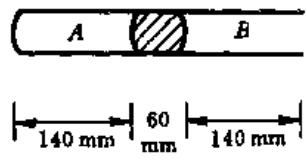
\includegraphics[width=0.25\textwidth]{figures/热图1-5-1.jpg}
\end{center}
\vfill

\textbf{1-6} 【题6】如热图1-6-1，一根均匀玻璃管长 $96\mathrm{cm}$ ，一端封闭，一端开口，竖直放置，开口端向上。管内有一

段长为 20 cm 的水银柱, 当温度为 27 ℃ 时, 水银柱下方被封闭的空气柱的长度为 60 cm, 外界的大气压强为 76 cmHg. 试问当温度升高到多少时, 水银柱刚好从管中全部溢出. 设玻璃管和水银因温度升高而产生的膨胀可忽略不计, 设外界大气压强始终保持不变, 设被封闭的空气可视为理想气体.
\begin{center}
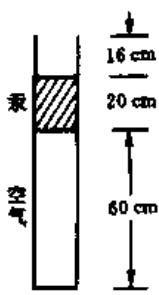
\includegraphics[width=0.3\textwidth]{figures/热图1-6-1.jpg}
\end{center}
\vfill

\newpage
\textbf{1-7} 【题7】如热图1-7-1，截面均匀，下端 $A$ 封闭的细长试管 $AB$ 竖直放置。管下端 $A$ 内封有长为 $L_{0}$ 的空气，管中间是长为 $L = 4L_{0}$ 的水银柱，管上端 $B$ 有长为 $L_{0}$ 的空气。开始时，管上端 $B$ 与大气连通，大气压强为 $p_0 = 2\rho gL$ ，其中 $\rho$ 为水银密度。

1. 如果先将 B 端封闭, 再将试管缓慢倒转 $180^{\circ}$ , 试问管中 A 端空气柱长度 $L_{A}$ 与 B 端空气柱长度 $L_{B}$ 各为多少 $L_{0}$ ?

2. 如果 $B$ 端始终与大气连通, 不封闭, 先将试管缓慢倒转 $180^{\circ}$ , 再缓慢回转 $180^{\circ}$ 复原. 试问最后管中 $A$ 端空气柱长度 $L_{A}^{\prime}$ 与 $B$ 端空气柱长度 $L_{B}^{\prime}$ 各为多少 $L_{0}$ ?

设倒转过程均在大气环境下进行,温度不变.

\begin{center}
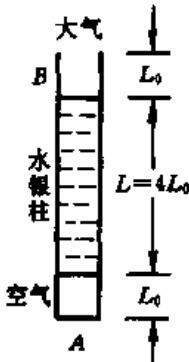
\includegraphics[width=0.15\textwidth]{figures/热图1-7-1.jpg}
\end{center}
\vfill

\textbf{1-8} 【题8】如热图1-8-1，一个装有进水孔 $a$ 和排水孔 $b$ 的铁制水箱，质量为 $840\mathrm{kg}$ ，容积为 $1\mathrm{m}^3$ 。此箱不

慎沉入湖底, 箱内充满了水, 排水孔 $b$ 与湖面相距 $10 \mathrm{~m}$ . 今采用充气法打捞水箱, 先将管子与进水孔 $u$ 连接, 用压气机把空气打进箱内, 使箱内的水排出一部分. 试问要打进多少体积的压强为 $1 \mathrm{atm}$ 、温度为 $27^{\circ} \mathrm{C}$ 的空气, 水箱才开始上浮? 设湖底的水温为 $7^{\circ} \mathrm{C}$ , 空气重量可略, 水箱铁壳的体积可略, 水的密度随湖深度的变化也可忽略.
\begin{center}
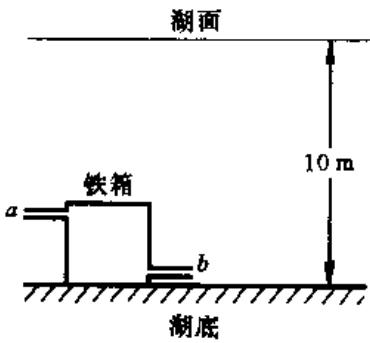
\includegraphics[width=0.25\textwidth]{figures/热图1-8-1.jpg}
\end{center}
\vfill

\newpage
\textbf{1-9} 【题9】一球形热气球,总质量(包括隔热很好的球皮以及吊篮等装载)为300 kg.经加热后,气球膨胀到最大体积,其直径为18 m.设球内外气体成份相同,球内气体压强稍高于大气压.已知大气温度为27 ℃,压强为1 atm,标准状态下空气的密度为1.3 kg/m³.试问热气球刚好能上升时,球内空气的温度应为多少?
\vfill

\textbf{1-10} 【题10】一薄壁圆柱形浮沉子一端封闭，一端开口。将开口端向下插入密度为 $\rho$ 的液体中，浮沉子内气体被封闭，当液体上方大气压强为 $p_0$ 时，闭端刚好与液面持平。若突然将液面上方压强增为 $2p_0$ ，试证明浮沉子下沉深度 $x$ 与它在该处运动速度 $v$ 的关系为

$$
v ^ {2} = 2 g x - \frac {2 p _ {0}}{\rho} \ln \left(1 + \frac {\rho g x}{2 p _ {0}}\right)
$$

其中 g 为重力加速度．设空气密度与 $\rho$ 相比可以忽略，空气可看作理想气体，不计任何粘滞阻力，且设液体内处处温度相同．
\vfill

\newpage
\textbf{1-11} 【题11】宇宙飞船投放的一个仪器以恒定速度垂直下落，接近并到达某行星的表面。该仪器用约定单位记录的压强 p 随时间 t 变化的曲线如热图1-11-1所示。落到行星表面时，该仪器还测出环境温度为 $T = 700 \, K$ ，行星表面自由落体加速度为 $g = 10 \, m/s^{2}$ 。已知该行星的大气由二氧化碳构成。试求仪器下落的速度 v。
\begin{center}
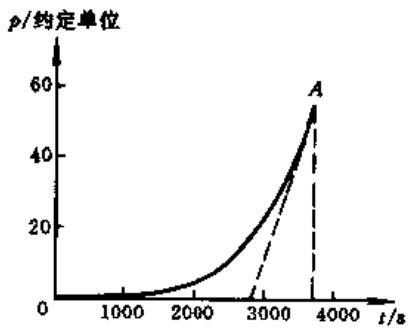
\includegraphics[width=0.25\textwidth]{figures/热图1-11-1.jpg}
\end{center}
\vfill

\textbf{1-12} 【题12】所谓某混合理想气体中各组分的体积百分比，是指各组分单独处在与混合理想气体相同压强与温度状态下，其体积在混合理想气体体积中所占的百分数。空气可当作理想气体，空气中几种主要组分的体积百分比是，氮 $(\mathbf{N}_2)78\%$ ，氧 $(\mathrm{O}_2)21\%$ ，氩（Ar） $1\%$ 。试求在标准状态(1atm, $0^{\circ}\mathrm{C}$ )下空气的密度。已知氮、氧、氩的分子量分别是28.0,32.0,39.9。
\vfill

\newpage
\textbf{1-13} 【题13】一块铝片先在干燥空气中测量质量，再在潮湿空气中测量质量。已知潮湿空气中水蒸气的分压为 $15.2\mathrm{mmHg}$ ，称质量时采用铜砝码，大气压强为 $760\mathrm{mmHg}$ ，在两种测量时温度相同为 $20^{\circ}\mathrm{C}$ 。如果所用称的灵敏度只能对 $0.1\mathrm{mg}$ 的差别才有反应，试问铝片至少应有多少质量才能在上述两种测量下表现出差别。

已知铝的密度为 $2.7 \, g/cm^{3}$ ，铜的密度为 $8.5 \, g/cm^{3}$ ， $20^{\circ}C$ 的空气的密度为 $0.0012 \, g/cm^{3}$ ，水蒸气的密度为 $0.00075 \, g/cm^{3}$ .
\vfill


\textbf{1-14}【题 14】由固态导热材料做成的长方体容器,被一隔板分成两个互不连通的部分,其中分别贮有相等质量的干燥空气和潮湿空气,在潮湿空气中水汽质量占2%.

1. 若隔板可自由无摩擦地沿器壁滑动。试求达到平衡后，干空气和湿空气所占体积的比值。

2. 若一开始采用能确保不漏气的方式将隔板抽出，试求达到平衡后容器内气体的压强，与未抽出隔板时干空气和湿空气各自的压强这三者的比值。

设干空气和湿空气均可视为理想气体。
\vfill
\newpage

\textbf{1-15}【题 15】如热图1-15-1所示,一端开口,另一端封闭的长圆柱形导热容器开口向上竖直放置.在气温为27℃,气压为760 mmHg,相对湿度(空气中水蒸气压强与该温度下饱和水蒸气压强的比值)为75%时,同一质量可忽略不计的光滑薄活塞将开口端封闭.已知水蒸气的饱和蒸汽压在27℃时为26.7 mmHg,在0℃时为4.58 mmHg.

试问:1. 若保持温度不变,通过在活塞上方注入水银增加压强的方法使管内开始有水珠出现,则容器至少应为多长?

2. 若在水蒸气刚开始凝结时固定活塞, 降低容器的温度, 则当温度降至 $0^{\circ}$ C 时, 容器内气体的压强为多大?
\begin{center}
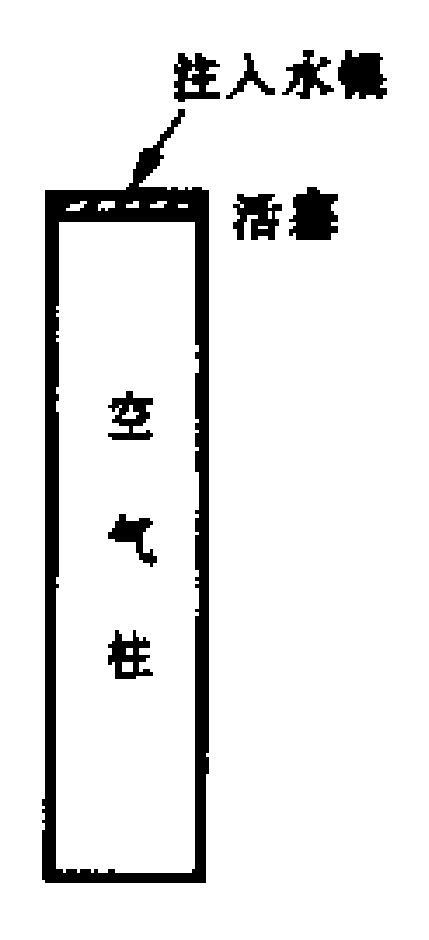
\includegraphics[width=0.08\textwidth]{figures/热图1-15-1.jpg}
\end{center}
\vfill

\textbf{1-16}【题16】如热图1-16-1，一根两端封闭、粗细均匀的石英管竖直放置，管内有一段水银柱，水银柱下方为空气，上方为一种可分解的双原子分子气体。这种双原子分子气体的性质是，当温度 $T > T_0$ 时，它的双原子分子开始分解为单原子分子。若用 $n_0$ 表示 $T_0$ 时的双原子分子数，用 $\Delta n$ 表示 $(T_0 + \Delta T)$ 时分解了的双原子分子数，则当 $\Delta T$ 很小时，分解遵循的规律为

$$
\frac {\Delta n}{n _ {0}} = \frac {\Delta T}{T _ {0}}
$$

已知初始温度为 $T_{0}$ ，此时下方空气柱的长度为 $2l_{0}$ ，上方气柱的长度为 $l_{0}$ ，水银柱产生的压强为下方空气柱压强的 $\alpha$ 倍 ( $0 < \alpha < 1$ )。设石英管和水银柱体积随温度的变化可以忽略。试问当温度由 $T_{0}$ 稍稍增加时, 水银柱将上升还是下降?

\begin{center}
    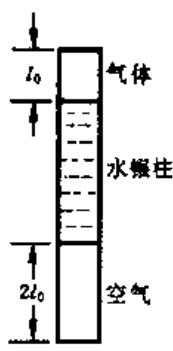
\includegraphics[width = 0.1\textwidth]{figures/热图1-16-1.jpg}
\end{center}

\vfill











\chapter{热力学定律}
\newpage
\textbf{2-1} 【题1】试证明如热图2-1-1所示的理想气体循环过程的比热 $c$ 必不为常量.
\begin{center}
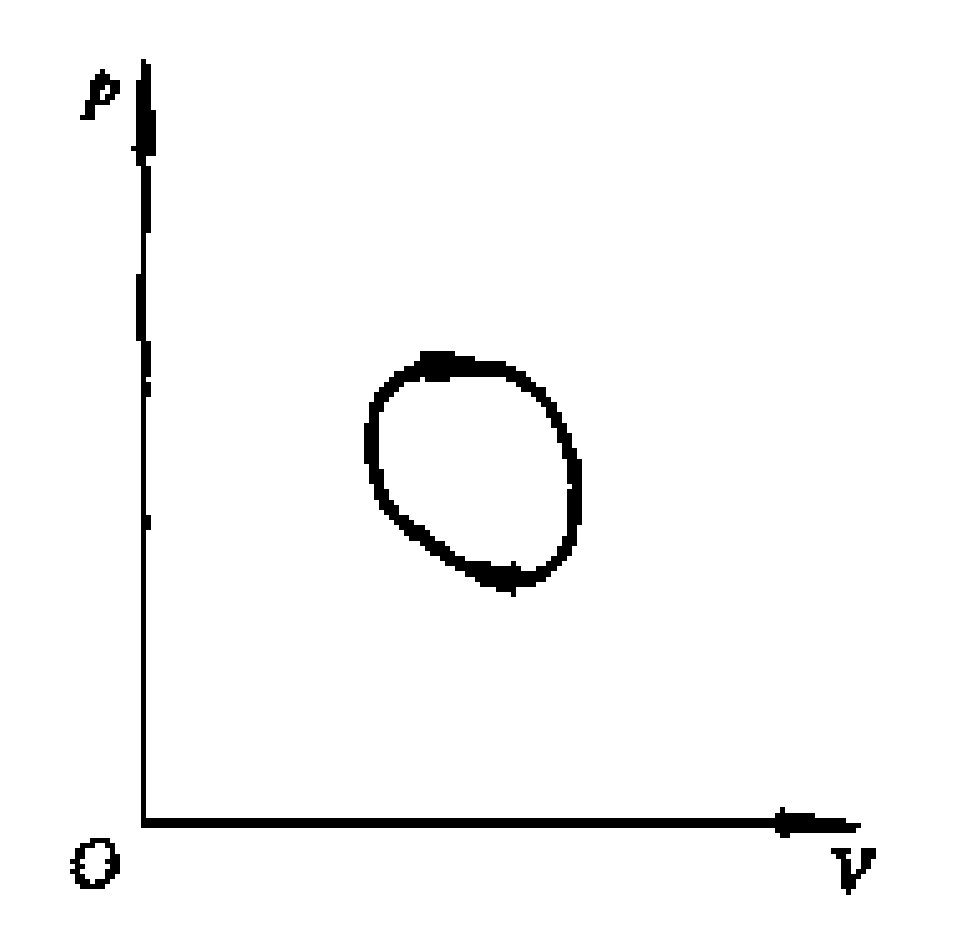
\includegraphics[width=0.2\textwidth]{figures/热图2-1-1.jpg}
\end{center}
\vfill

\textbf{2-2} 【题2】摩尔质量为 $\mu$ ，等体比热为 $c_{\mathrm{V}}(c_{\mathrm{V}}$ 为常量)的理想气体所经历的 $x$ 过程如热图2-2-1所示．若在此 $p - V$ 坐标面上，把上述 $x$ 过程向下平移 $p_0(p_0 > 0)$ ，则所得之曲线刚好是该理想气体温度为 $T_{0}$ 的等温过程．

1. 试确定 $x$ 过程中的温度下限，并指明该温度在 $x$ 过程曲线的哪个部位。

2. 试导出 $x$ 过程中比热 $c$ 与压强 $p$ 的定量关系, 并画出 $c \sim p$ 曲线.

\begin{center}
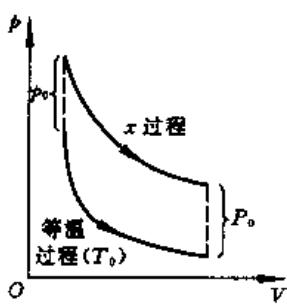
\includegraphics[width=0.2\textwidth]{figures/热图2-2-1.jpg}
\end{center}
\vfill

\newpage
\textbf{2-3} 【题3】质量为 $M$ ，摩尔质量为 $\mu$ ，等体比热为 $c_{V} = \frac{3R}{2\mu}$ 的理想气体经历的直线过程如热图2-3-1所示.

1. 试确定此过程的 $T - V$ 关系，并画图。

2. 试确定此过程中比热 $c$ 与体积 $V$ 之间的关系, 画出曲线, 并依据 $c = \frac{\mathrm{d} Q}{M \mathrm{~d} T}$ 对各段曲线 $c$ 值的正、负作定性解释.

\begin{center}
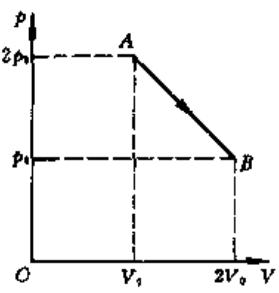
\includegraphics[width=0.2\textwidth]{figures/热图2-3-1.jpg}
\end{center}
\vfill

\textbf{2-4} 【题4】由 $\nu_{1}$ 摩尔的单原子分子理想气体与 $\nu_{2}$ 摩尔的双原子分子理想气体混合组成某种理想气体，已知该混合理想气体在常温下的绝热方程为

$$
p V ^ {\frac {1 1}{7}} = \text { 常量 }
$$

试求 $\nu_{1}$ 与 $\nu_{2}$ 的比值 $\alpha$ .
\vfill

\newpage
\textbf{9-5} 【题5】1 mol单原子分子理想气体经历某准静态过程，初态为 $(4p_0, V_0)$ ，终态为 $\left(\frac{p_0}{4}, 8V_0\right)$ . 已知在此过程的每一小过程中热功效率 $\frac{\mathrm{d}W}{\mathrm{d}Q}$ 均相同。试求此过程中气体对外界所作总功 $W$ 。
\vfill

\textbf{2-6} 【题6】2 mol单原子分子理想气体从某初态经历热容量为 $C=2R(1+0.01T)$ 的准静态过程，到达温度为初态温度2倍、体积为初态体积 $\sqrt{2}$ 倍的终态。试求内能增量 $\Delta U$ 及系统对外所作的功 W。
\vfill

\newpage
\textbf{2-7} 【题7】空气是混合气体,其中的质量分配是,氮气约占 $76.9\%$ , 氧气约占 $23.1\%$ , 其余成分可忽略不计. 现有一气缸, 缸内充有空气, 并装有一些由细钢丝做成的钢丝棉. 设气缸内的活塞能无摩擦地运动, 设缸内气压恒定为 $1 \mathrm{atm}$ . 设缸内非常缓慢地进行化学反应, 设化学反应生成 $1 \mathrm{mol}$ 的 $\mathrm{Fe}_{2} \mathrm{O}_{3}$ 后, 因氧气耗尽而中止. 已知化学反应过程是在 $1 \mathrm{atm}, 300 \mathrm{~K}$ 条件下进行的, 在此过程中系统释放出 $8.24 \times 10^{5} \mathrm{J}$ 的热量.

试求在此过程中:1. 系统内能的改变量.2. 缸内气体内能的改变量.3. 缸内氮气密度的改变量.

设缸内气体可视为理想气体．设1 mol氧气和1 mol氮气的内能均为 $\frac{5}{2}RT$ ．设缸内钢丝棉等固态物质与缸内气体相比，所占体积很小，可忽略不计．
\vfill

\textbf{2-8} 【题8】如热图2-8-1，一固定的直立气缸，它由上、下两个相互连通的圆筒构成。上部圆筒的体积为 $V_{m}$ ，其中有一个质量为 $2m$ 、面积为 $2S$ 的薄活塞A。下部圆筒足够长，其中有一个质量为 $m$ 、面积为 $S$ 的活塞B。两圆筒由一细而短的管道连通，两活塞均可在各自的圆筒内无摩擦地上下滑动，活塞A的上方盛有 $1\mathrm{mol}$ 的理想气体，活塞A、B之间盛有某种气体，活塞B下方与大气连通。开始时整个系统处于平衡态，A上方理想气体的温度为 $T_{0}$ ，已知该理想气体每摩尔的内能 $U = CT$ ，其中 $C$ 为常量， $T$ 为热力学温度，活塞B下方的大气压强为常量 $p_{0}$ ，设气缸壁、管道、活塞均不导热。然后，通过置于上部圆筒顶端的电热丝 $L$ 对活塞A上方的气体缓慢加热，设在整个加热过程中传递给A上方气体的热量为 $Q_{0}$ 。试问达到平衡时，A上方气体的温度 $T_{f}$ 是多少？
\begin{center}
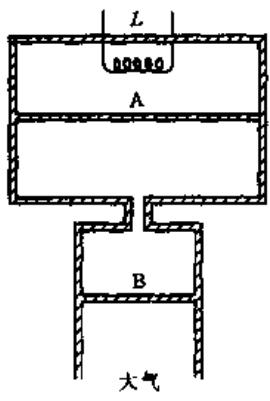
\includegraphics[width=0.15\textwidth]{figures/热图2-8-1.jpg}
\end{center}
\vfill

\newpage
\textbf{2-9} 【题9】如热图2-9-1，A和B是两个圆筒形绝热容器，中间用细的短管连通，短管中有导热性能良好的阀门 K, 短管与阀门对外绝热. F 是带柄的绝热活塞, 与容器 A 的内表面紧密接触, 不漏气, 且摩擦可忽略不计.

开始时 K 关闭, F 处于 A 的左端. A 中有 n 摩尔理想气体, 温度为 $T_{0}$ ; B 中为真空. 现在向右推动 F, 直到 A 中气体的体积与 B 的容积相等. 在此过程中, 已知对气体作功为 W, 气体温度升为 $T_{1}$ , 然后将 K 稍稍打开一点, 使 A 中的气体缓慢地向 B 扩散, 同时让活塞 F 缓慢地前进, 并保持 A 中活塞 F 附近气体的压强近似不变. 试问在此过程中, 气体最后的温度是多少? 设活塞、阀门、容器的热容量均可不计.
\begin{center}
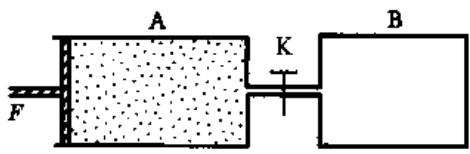
\includegraphics[width=0.3\textwidth]{figures/热图2-9-1.jpg}
\end{center}
\vfill

\textbf{2-10} 【题10】如热图2-10-1，在一以绝热壁包围的刚性圆柱形封闭气缸内，装着一个有小阀门 $L$ 的绝热活塞，在气缸的 $A$ 端还装有电热器 $\mathbf{H}$ ，可用于加热气体。

开始时, 活塞紧贴气缸 B 端的内壁, 小阀门 L 关闭. 整个气缸内装有一定质量的理想气体, 其温度为 $T_{0}$ . 然后设法把活塞推到气缸中央, 设活塞与气缸壁之间的摩擦可以忽略, 并用销钉 F 将活塞固定住, 这样气缸被分成体积相等的左、右两室, 如热图2-10-1所示. 在上述压缩气体的过程中, 设外界对气体作功 W, 气体温度上升到 T.

再开启小阀门,经过足够长时间后关闭,并拔去销钉使活塞可以自由移动．用电热器加热气体，加热完毕并经过一定时间后，测出左室气体压强增为加热前的1.5倍，右室的体积变为原来的0.75倍．试求电热器传递给气体的热量．
\begin{center}
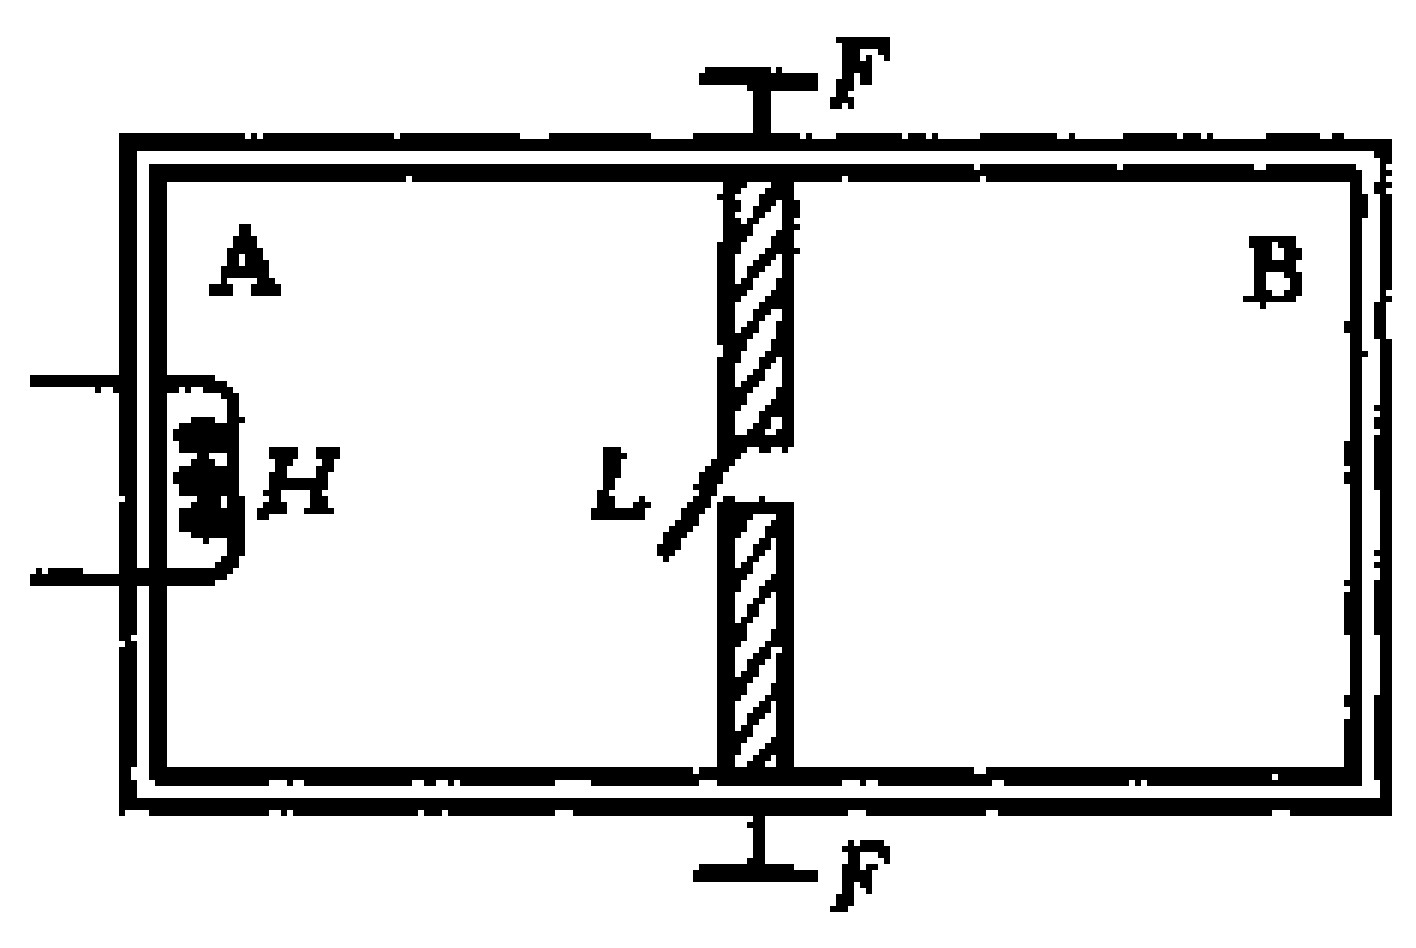
\includegraphics[width=0.2\textwidth]{figures/热图2-10-1.jpg}
\end{center}
\vfill

\newpage
\textbf{2-11} 【题11】如热图2-11-1，两个底面积均为 $S = 100\mathrm{cm}^2$ 的圆筒．左筒内气体的质量 $M_{\text{左}} = 4\mathrm{g}$ ，体积 $V_{左}=22.4L$ ，压强 $p_{左}=1\ atm$ ，温度 $T_{左}=273\ K$ 。右筒内有同种气体，质量 $M_{右}=7.44\ g$ ，体积 $V_{右}=22.4L$ ，温度 $T_{右}=273\ K$ 。左筒筒壁绝热，右筒靠大热库维持恒定的 $0\ ^{\circ}C$ 的温度。整个系统在真空中，放开左、右筒相联的活塞后，活塞移动了 $l=50\ cm$ 后达到平衡而静止。试问右筒内的气体吸收了多少热量？已知气体可视为理想气体，其定容比热为 $c_{V} = 0.75\mathrm{cal}^{*} / (\mathrm{g}\cdot \mathrm{K}) = 3.14\mathrm{J} / (\mathrm{g}\cdot \mathrm{K})$ ，设活塞与筒壁之间无摩擦。
\begin{center}
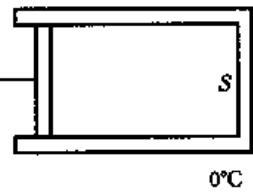
\includegraphics[width=0.2\textwidth]{figures/热图2-11-1.jpg}
\end{center}
\vfill

\textbf{2-12} 【题12】如热图2-12-1，底面积为 $100\mathrm{cm}^2$ 的圆筒，筒壁、活塞以及内部隔板都是完全绝热的。当筒内右方压强大于左方时，隔板的阀门打开。开始时有12g氮气在左方，有2g氮气在右方，左、右两方的长度均为112cm，温度均为0℃。外部压强为 $10^{5}$ Pa。氦气定体比热 $c_{V}=3.15\mathrm{J}/(\mathrm{g}\cdot\mathrm{K})$ ，定压比热为 $c_{p}=5.25\mathrm{J}/(\mathrm{g}\cdot\mathrm{K})$ 。今把活塞缓慢地推向隔板，当阀门打开时稍停片刻，尔后继续缓慢地推动活塞，直至到达隔板为止。设氮气可看作理想气体，各过程可看作准静态过程，忽略摩擦。试求所作的总功。
\begin{center}
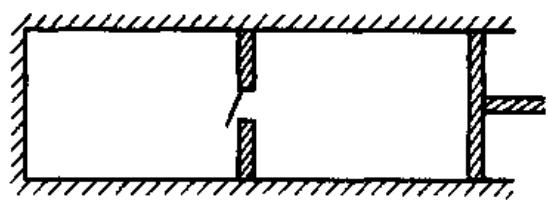
\includegraphics[width=0.25\textwidth]{figures/热图2-12-1.jpg}
\end{center}
\vfill

\newpage
\textbf{2-13} 【题13】如热图2-13-1, 长为 $2L$ 的长方形绝热容器被一个可以无摩擦地自由滑动的活塞分为容积相等的两部分 A 和 B, A 和 B 内各装有相同摩尔的单原子分子理想气体, 温度相同, 压强均为一个大气压. 今将活塞缓慢地向左推移, 当活塞移过 $\frac{1}{2}$ 时便停住, 再将活塞上的阀门打开, 使两边的气体混合. 试求容器内气体的最终压强 $p$ .
\begin{center}
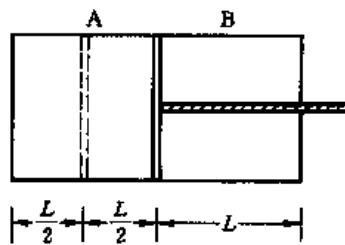
\includegraphics[width=0.2\textwidth]{figures/热图2-13-1.jpg}
\end{center}
\vfill
\newpage

\textbf{2-14} 【题14】如热图2-14-1，潮湿空气绝热地持续流过山脉．气象站 $M_0$ 和 $M_3$ 测出的大气压强都是100kPa, 气象站 $M_{2}$ 测出的大气压强为 70 kPa. 在 $M_{0}$ 处, 空气的温度是 20 ℃, 随着空气的上升, 在压强为 84.5 kPa 的高度处 (图中 $M_{1}$ ) 开始有云形成. 空气由此继续上升, 经 1500 s 之后到达山顶的 $M_{2}$ 站. 在上升过程中, 空气里的水蒸气凝结成雨落下. 设每平方米上空潮湿空气的质量为 2000 kg, 每千克潮湿空气中凝结出 2.45 g 的雨水.

1. 试求出在云层底部高度处(图中 $M_{1}$ ) 的温度 $T_{1}$ .

2. 假定空气密度随高度线性地减少, 试问云层底部 $M_{1}$ 与 $M_{0}$ 的高度差 $h_{1}$ 是多少?

3. 试问在山顶 $M_{2}$ 处测出的温度 $T_{2}$ 是多少？

4. 试求出由于空气中水蒸气的凝结, 在 3 小时内形成的降雨量. 设在 $M_{1}$ 和 $M_{2}$ 之间降雨是均匀的.

5. 试问在山脉背面的气象站 $M_{3}$ 测出的温度 $T_{3}$ 是多少？讨论 $M_{3}$ 处空气的状态，并与 $M_{0}$ 处相比较。

提示和数据:空气可看作是理想气体.水蒸气对空气热容量和密度的影响均可忽略.同样,汽化热随温度的变化也可忽略.温度的计算应精确到1K,云层底部高度的计算应精确到10m,降雨量的计算应精确到1mm.在有关的温度范围内,空气的定压比热为 $C_{p}=1005\ \mathrm{J}/(\mathrm{kg}\cdot\mathrm{K})$ .在 $M_{0}$ 处,相应于 $p_{0}$ 和 $T_{0}$ 的空气密度为 $\rho_{0}=1.189\ kg/m^{3}$ .在云层中,水的汽化热为 $L_{V}=2\ 500\ kJ/kg$ .又, $\frac{C_{p}}{C_{V}}=\gamma,\gamma=1.4,g=9.81\ m/s^{2}$ .
\begin{center}
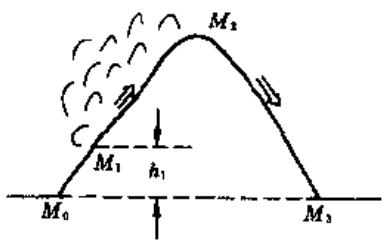
\includegraphics[width=0.25\textwidth]{figures/热图2-14-1.jpg}
\end{center}
\vfill

\newpage
\textbf{2-15} 【题15】在两端开口的竖直 $U$ 形管中注入水银，水银柱的全长为 $h$

1. 将一边管中的水银下压, 静止后撤去所加压力, 水银便会振荡起来. 试证明, 不计摩擦时, 振动周期为 $T_{1} = 2 \pi \sqrt{\frac{h}{2g}}$ .

2. 把管的右端封闭, 设被封在右管内的空气柱的高度为 $L$ , 然后使水银柱作微小的振荡, 仍设摩擦可忽略, 设空气为理想气体, 且可认为水银柱振荡时右管内被封闭的空气经历的是准静态绝热过程. 试证明, 振动周期为

$$
T _ {2} = 2 \pi \sqrt {\frac {h}{2 g + \gamma h _ {0} \frac {g}{L}}}
$$

式中 $h_{0}$ 为用水银计测量大气压的水银柱的高度, $\gamma$ 是空气的绝热指数.

3. 试证明, $\gamma = \frac{2L}{h_0}\left(\frac{T_1^2}{T_2^2} - 1\right)$ .
\vfill

\textbf{2-16} 【题16】声波可在气体管中形成驻波。现用 $1000\mathrm{Hz}$ 的声波在碘蒸气管中做实验，在温度为 $400\mathrm{K}$ 时，测得管内形成的驻波的相邻间距为 $6.77~\mathrm{cm}$ ，试问管内的碘蒸气分子是单原子的还是双原子的．已知碘的原子量是127，声波在空气中的传播速度 $v=\frac{1}{\sqrt{\rho K_{s}}}$ ，其中 $\rho$ 为气体的密度， $K_{s}$ 为气体的绝热压缩系数，定义为 $K_{s}=-\frac{1}{V}\left(\frac{dV}{dp}\right)_{绝热}$
\vfill

\newpage
\textbf{2-17} 【题17】定体摩尔热容量 $C_V$ 为常量的某理想气体。经历如热图2-17-1所示的 $pV$ 平面上的两个循环过程 $A_1B_1C_1A_1$ 和 $A_2B_2C_2A_2$ ，相应的效率分别为 $\eta_1$ 和 $\eta_2$ 。试比较 $\eta_1$ 与 $\eta_2$ 的大小（用不等式或等式表示）。
\begin{center}
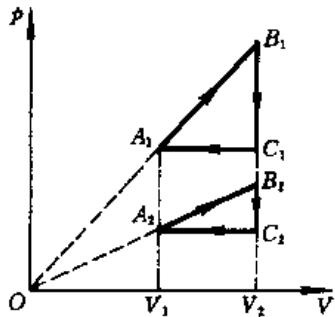
\includegraphics[width=0.2\textwidth]{figures/热图2-17-1.jpg}
\end{center}
\vfill

\textbf{2-18} 【题18】如热图2-18-1，在 $p \quad V$ 平面上用实线画出了 $C_V$ 为常量的某理想气体的几条准静态过程线，其中两条实曲线是绝热过程，三条实直线是直线过程，其延长线交于原点 $O$ 。

1. 试比较 $\eta_{12431}$ (循环过程12431的效率, 余同)与 $\eta_{12651}$ 的大小.

2. 设 $p_1^*: p_2^*: p_3^* = 1:2:3$ ，试比较 $\eta_{12431}$ 与 $\eta_{34651}$ 的大小。
\begin{center}
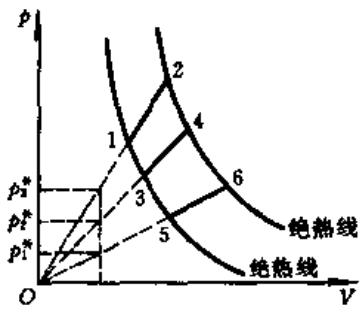
\includegraphics[width=0.2\textwidth]{figures/热图2-18-1.jpg}
\end{center}
\vfill

\newpage
\textbf{2-19} 【题19】 $1\mathrm{mol}$ 氦气(理想气体)经历如热图2-19-1所示的循环过程，热图2-19-1中AB、

BC、CA 均为直线, 有关参量已经标明. 试求循环效率 $\eta$ .

\begin{center}
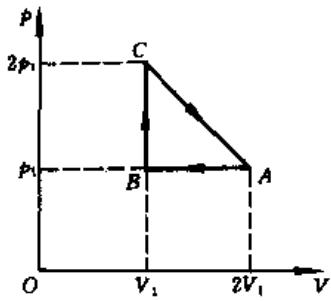
\includegraphics[width=0.2\textwidth]{figures/热图2-19-1.jpg}
\end{center}
\vfill

\textbf{2-20} 【题20】如热图2-20-1，$0.1\mathrm{mol}$ 单原子分子理想气体从初态 $(p_0 = 32.0\mathrm{Pa},V_0 = 8.00\mathrm{m}^3)$ 经 $p - V$ 图上的直线过程到达终态 $(p_{1} = 1.0\mathrm{Pa},V_{1} = 64.0\mathrm{m}^{3})$ ，再经绝热过程回到初态，试求:

1. 循环效率.

2. 上述循环的最高温度和最低温度.

\begin{center}
    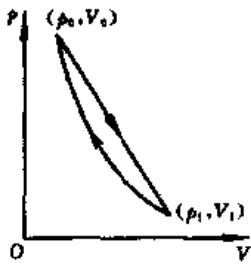
\includegraphics[width = 0.2\textwidth]{figures/热图2-20-1.jpg}
\end{center}

\vfill


\chapter{气体动理论}
\newpage
\textbf{3-1} 在一个密闭容器内盛有水，未满，处于平衡状态。已知水在 $14^{\circ}\mathrm{C}$ 时的饱和蒸汽压为 $12.0\mathrm{mmHg}$ 。设水蒸气分子碰到水面后，都能进入水内，设饱和水蒸气可看作理想气体。试问在 $100^{\circ}\mathrm{C}$ 和 $14^{\circ}\mathrm{C}$ 时，单位时间内通过单位面积水面蒸发成为水蒸气的分子数之比 $n_{100}:n_{14}$ 为多大（取2位有效数字）。
\vfill

\textbf{3-2} 如热图3-2-1，一块平而薄的长方形匀质玻璃板，用两根质量可略的等长细线悬挂起来, 玻璃板两个表面的半个面分别对称地涂了一层化学性质活泼的金属, 整个装置放在容器之中, 容器内有压强为 $p$ 的氯气。

设每一个氯气分子遇到金属分子后发生化学反应的概率为 $q(q < 1)$ ，且 $q$ 为恒量。设玻璃板两边的氯气密度相等。设在化学反应过程中，氯气压强的减小可忽略不计。设玻璃板的质量为 $m$ ，有关几何量如热图3-2-1所标示。

观察到玻璃板绕它的竖直轴转过一个很小的角度 $\alpha$ 后, 处于平衡状态. 试求 $\alpha$ 的大小.
\begin{center}
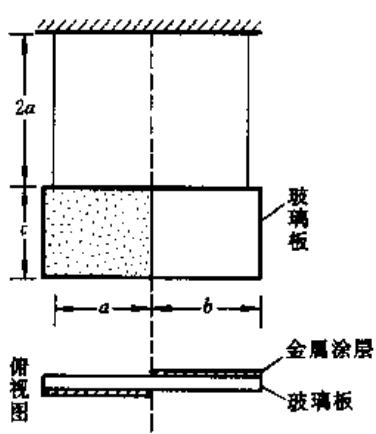
\includegraphics[width=0.2\textwidth]{figures/热图3-2-1.jpg}
\end{center}
\vfill

\newpage
\textbf{3-3} 如热图3-3-1，在真空中有一个质量为 $M$ 的试管，它被质量为 $m$ 的隔板等分为两部分。隔板封闭的那部分有质量为 $n\mathrm{mol}$ , 温度为 $T$ , 摩尔质量为 $\mu$ 的单原子分子理想气体. 放开隔板后, 隔板无摩擦地直立向上移动, 在隔板离开试管顶端后气体方始从试管逸出. 设隔板开始运动时, 试管静止. 试求试管的最终速度.

设重力可忽略。设气体、隔板、试管三者之间的热量交换可忽略。设在隔板离开试管前，气体经历准静态过程。
\begin{center}
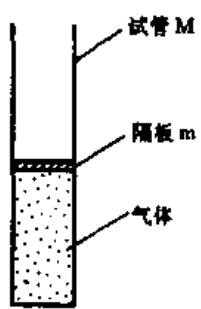
\includegraphics[width=0.15\textwidth]{figures/热图3-3-1.jpg}
\end{center}
\vfill

\textbf{3-4} 在一柱形容器内，有大量相同的小球沿着容器的长度方向往返运动。小球可视为质点，小球之间以及小球与容器端面(与其长度方向垂直)之间作弹性碰撞。小球的速率以及向前还是向后运动都是无规的。可引入"温度"T的概念，它是由小球的平均动能 $\varepsilon$ 定义的，为 $\bar{\varepsilon}=\frac{1}{2}kT$ ，式中k是玻尔兹曼常数。今在容器的一端安装平面弹性活塞，并使活塞缓慢地沿容器长度方向向内推进，运动的小球因与活塞作弹性正碰撞增加了动能，从而使系统的"温度"升高。

上述模型实际上就是单原子分子理想气体一维热运动绝热压缩的微观模型。

试导出在活塞缓慢推进过程中，"温度"T与体积V的关系式(此即单原子分子理想气体的一维绝热过程方程).设重力,引力,各种阻力和摩擦力均可忽略.
\vfill

\newpage
\textbf{3-5} 空腔内的热辐射可以当作光子气来处理．设腔的内表面对光子是完全反射面．

1. 如果在某温度下，腔内热辐射已处于平衡状态，此时光子气的能量密度为 u。试求光子气的压强 p。

2. 试证明 $u$ 只是温度 $T$ 的函数。

3. 试证明 $p \propto T^4$ .

4. 试导出光子气在绝热过程中压强 $p$ 与空腔体积 $V$ 之间满足的关系式(绝热过程方程).
\vfill

\textbf{3-6} 混合理想气体处于温度为 $T$ 的平衡态, 其中任意两个质量分别为 $m_{1}$ 和 $m_{2}$ 的分子之间的相对速度定义为 $\pmb{u} = \pmb{v}_{1} - \pmb{v}_{2}$ , 式中 $\pmb{v}_{1}$ 和 $\pmb{v}_{2}$ 分别是 $m_{1}$ 和 $m_{2}$ 的速度. 试求: 相对速率的方均根值和平均值, 即求 $\sqrt{\overline{u^2}}$ 和 $\overline{u}$ .
\vfill

\newpage
\textbf{3-7} 理想气体处于平衡态，其分子平动动能表为 $E$ ，分子最概然平动动能表为 $E_{\mathrm{p}}$ ，与 $E_{\mathrm{p}}$ 相应的平动速率表为 $v_{0}$ ，试求 $v_{0}$ 与最概然速率 $v_{\mathrm{p}}$ 的比值.
\vfill

\textbf{3-8} 设热气球具有不变的容积 $V_{B} = 1.1 \, \mathrm{m}^{3}$ ，气球蒙皮体积与 $V_{B}$ 相比可忽略不计，蒙皮的质量为 $m_{H} = 0.187 \, \mathrm{kg}$ 。在外界气温 $t_{1} = 20 \, ^{\circ}\mathrm{C}$ ，正常外界大气压 $p_{1} = 1.013 \times 10^{5} \, \mathrm{Pa}$ 的条件下，气球开始升空，此时外界大气的密度为 $\rho_{1} = 1.2 \, \mathrm{kg/m}^{3}$ 。

1. 试问气球内部的热空气的温度 $t_2$ 应为多少, 才能使气球刚好浮起.

2. 先把气球系牢在地面上，并把其内部的空气加热到稳定温度 $t_{3} = 110^{\circ}\mathrm{C}$ ，试问气球释放升空时的初始加速度 a 等于多少？(不考虑空气的阻力。)

3. 将气球下端通气口扎紧，使气球内部的空气密度保持恒定。在内部空气保持稳定温度 $t_{3} = 110^{\circ}\mathrm{C}$ 的情况下，气球升离地面，进入温度恒为 $20^{\circ}\mathrm{C}$ 的等温大气层中。试问，在这些条件下，气球上升到多少高度 h 能处于力学平衡状态。

4. 在上升到第3问中的高度 $h$ 时, 将气球在竖直方向上拉离平衡位置 $10 \mathrm{~m}$ , 然后再予以释放. 试定性叙述气球将作何种运动.
\vfill

\newpage
\textbf{3-9} 取地面为重力势能零点．试估算等温大气的重力势能与热运动能量之比．设大气分子都只有平动和转动的动能已被激发．
\vfill

\textbf{3-10} 把大气看作理想气体，设在大气范围内重力加速度 $g$ 为常量，设海平面 $z = 0$ 处的大气温度为 $T_{0}$

1. 从力平衡观点出发, 试导出 $z$ 处压强随高度的变化率 $\frac{\mathrm{d}p}{\mathrm{d}z}$ 与 $z$ 处的压强 $p$ 和温度 $T$ 的关系.

2. 设大气是等温的，且 $t_{0}=0^{\circ}\mathrm{C}$ ，试计算半数分子处于其下的高度 h.

3. 设大气是绝热的, 且 $t_0 = 0$ ℃, 绝热指数 $\gamma = \frac{7}{5}$ . 试计算大气层的高度 $H$ .
\vfill

\newpage
\textbf{3-11} 设地球的大气等温，温度为 $T$ ，地面附近的分子数密度为 $n_0$ ，大气分子的平均质量为 $m$ .如果认为，在距地面高度为 $\pmb{h}$ 处的大气分子沿某方向（当然不包括会与地面相碰的那些方向）的速度，达到或超过该处人造卫星绕地球作圆运动的速度（在不计空气阻力条件下）时，该分子便能沿此方向逃离大气而去．设地球半径为 $\pmb{R}$ ，地面的重力加速度为 $\pmb{g}$ 试求在 $\pmb{h}$ 处，沿任一允许方向,单位时间通过单位垂直截面逃离大气的分子数.
\vfill

\textbf{3-12} 一根长为 $L$ 的水平粗管与一根竖直细管连接成如热图3-12-1所示的形状。把细管下端插入密度为 $\rho_{f}$ 的液体之中，然后将粗管的管口封住，并使粗管绕细管以恒定的微小角速度 $\omega$ 旋转。已知空气的密度为 $\rho_{u}$ ，细管的体积与粗管相比可以忽略，毛细现象也可忽略。在温度恒定的条件下，试求细管中液面上升的高度 $h$ 。
\begin{center}
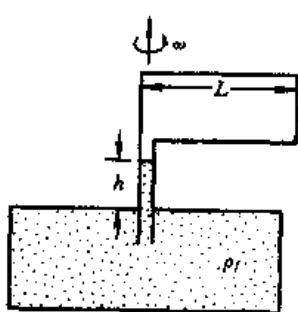
\includegraphics[width=0.2\textwidth]{figures/热图3-12-1.jpg}
\end{center}
\vfill

\newpage
\textbf{3-13} 原子序数为 $Z$ ，原子量为 $A$ 的单质气体，完全电离后形成的等离子体在均匀引力场 $\pmb{g}$ 中处于热平衡状态。设气体密度很小，电离后正、负离子间的局域相互作用可以忽略。

1. 在等温条件下,为了避免宏观的电荷分离(即正离子的数密度与负离子的数密度之比不因位置而变化),试证明必须有均匀电场 $E = -\frac{Am_{p} - m_{e}}{(1 + Z)e}g$ 存在.其中 $m_{p}$ 和 $m_{e}$ 分别是质子和电子的质量.

2. 如果不等温, 但各正、负离子受到的因热运动相互碰撞引起的平均力可认为相同, 试证明也必须有第 1 问的电场 E 存在.

3. 太阳表面附近存在着等离子体, 设其厚度远小于太阳半径, 设太阳表面有均匀分布的电荷 $Q$ , 试在等温、不等温条件下分别求 $Q$ 值.

4. 设太阳表面附近的等离子体是由氢原子电离产生的。试计算 $Q$ 值。已知太阳质量 $M = 2.0 \times 10^{30} \mathrm{~kg}$ 。
\vfill

\textbf{3-14} 从分子某次与其他分子碰撞后开始计算其自由程 $\lambda$ ，它的平均值 $\bar{\lambda}$ 称为平均自由程。设分子间的碰撞具有无后效应性，即在 $\lambda$ 到 $(\lambda + d\lambda)$ 区间与其他分子碰撞的概率与前面已经过的路程 $\lambda$ 无关。试求:

1. 分子经 $\lambda$ 路程尚未被碰撞的概率 $F(\lambda)$ ，以及分子自由程为 $\lambda$ 的概率密度（也称为自由程的分布函数） $f(\lambda)$ .

2. 分子在某次碰撞后, 先经无碰撞的路程 $\lambda_0$ , 再经 $\lambda$ 路程未被碰撞的概率 $F^*(\lambda_0, \lambda)$ , 以及不计 $\lambda_0$ 的平均自由程 $\bar{\lambda}(\lambda_0)$ .
\vfill

\newpage
\textbf{3-15} 理想气体处于平衡态, 分子热运动平均速率为 $\bar{v}$ , 平均自由程为 $\bar{\lambda}$ , 把 $t = 0$ 时刻某分子所在位置取为坐标原点 O. 试问经过多长时间 t, 该分子所在位置与原点 O 相距为 R.设理想气体占据的容器空间足够大, 设 $R \gg \bar{\lambda}$ , 设该分子在本题讨论的时间范围内未与容器壁相碰.最后, 已知 $\bar{v} = 5.0 \times 10^{2} \, \mathrm{m/s}, \bar{\lambda} = 3.0 \times 10^{-7} \, \mathrm{m}, R = 2 \, \mathrm{m}$ , 试给出 t 的具体数值.
\vfill

\textbf{3-16} 某混合理想气体包含A和B两种分子，已知A和B分子的质量、有效直径和数密度分别为 $m_{\mathrm{A}}$ 和 $m_{\mathrm{B}}, d_{\mathrm{A}}$ 和 $d_{\mathrm{B}}$ 以及 $n_{\mathrm{A}}$ 和 $n_{\mathrm{B}}$ 。试求在温度为 $T$ 的平衡态，两种分子各自的平均自由程 $\bar{\lambda}_{\mathrm{A}}$ 和 $\bar{\lambda}_{\mathrm{B}}$ 。
\vfill

\newpage
\textbf{3-17} 在阴极射线管中，即使管腔被抽成很高的真空度，也总是还有一些残余的空气存在。因此，从阴极射出的高速电子在通过管腔时，总有一部分因与空气分子相碰而不能直接射到荧光屏上。设阴极射线管工作时，管腔内的温度为 $27^{\circ}\mathrm{C}$ ，管腔的长度为 $20\mathrm{cm}$ 。为了保证有 $90\%$ 的电子能够不经碰撞直接射到屏上，试问管腔需抽到多高的真空度（用管腔内空气的压强表示）。已知空气分子的有效直径为 $3.0 \times 10^{-10}\mathrm{m}$ 。
\vfill

\textbf{3-18} 设气体分子的热运动速度分布在速度空间具有球对称性，速率分布函数为 $f(v)$ ，分子数密度为 $n$ 。试证明:

1.速率在 v 到 $\left(v + dv\right)$ 的分子, 单位时间与单位面积容器壁碰撞的分子数为 $\frac{1}{4}\left(nf(v)\mathrm{d}v\right)v$.

2. 全部气体在单位时间内与单位面积容器壁碰撞的分子数为 $\frac{1}{4} n\bar{v}$ , 其中 $\bar{v}$ 的分子的平均速率.
\begin{center}
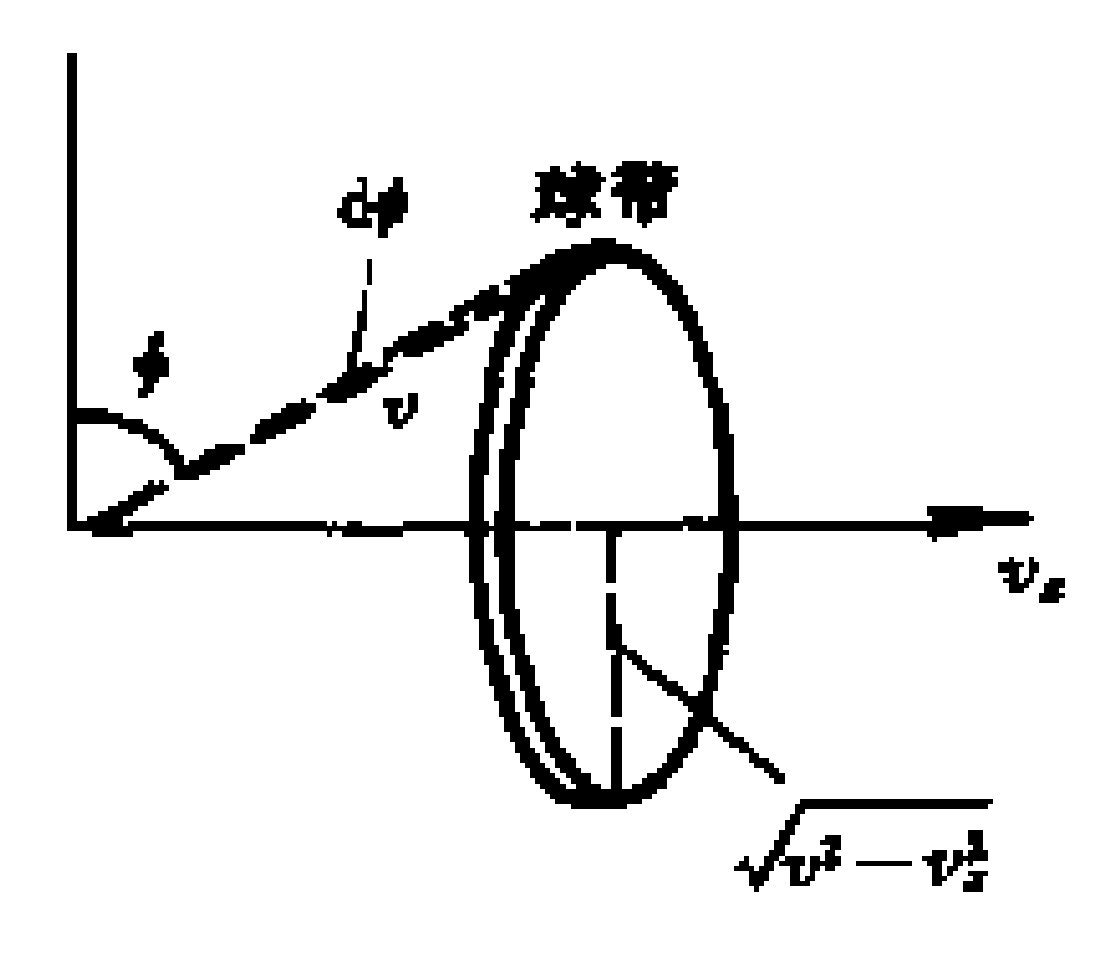
\includegraphics[width=0.3\textwidth]{figures/热图3-18-1.jpg}
\end{center}
\vfill

\newpage
\textbf{3-19} 如热图3-19-1,在温度为 $1000^{\circ}\mathrm{C}$ 的真空加热室中蒸发产生的铍原子(原子量为 9)气体经小孔逸出,透过准直狭缝形成原子束后,进入长度为 1 m 的真空大容器中,容器的右壁与原子束垂直.

1. 试求原子束中原子的速率分布, 平均速率和方均根速率.

2. 原子束中的原子进入真空容器后，将与残存的稀薄空气分子发生碰撞。设原子束行进1 m 后, 其强度(单位时间内通过的原子数) 减小为原来的 $\frac{1}{e}$ . 已知真空容器的温度为 300 K, 铍原子与空气分子的碰撞截面为 $10^{-20} ~\mathrm{m}^{2}$ , 忽略铍原子之间的碰撞. 试问真空容器中残存空气的压强是多少?

3. 铍原子每行进 1 m 所需的平均时间 $\bar{\tau}$ 是多少?

4. 设铍原子束刚进入真空容器时的粒子数密度为 $n_0 = 10^{10} \mathrm{~cm}^{-3}$ , 设铍原子与容器壁作完全非弹性碰撞. 试估计因铍原子束与容器壁碰撞对后者所施加的压强.
\begin{center}
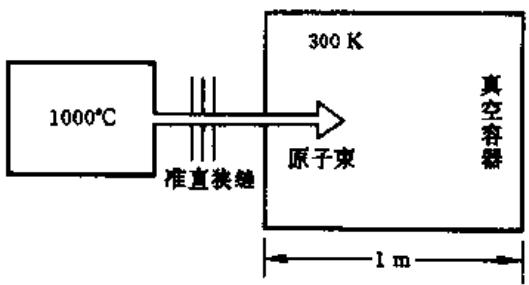
\includegraphics[width=0.3\textwidth]{figures/热图3-19-1.jpg}
\end{center}
\vfill
\newpage

\textbf{3-20} 在气象学中，降雨量是指雨区地面雨水的累加高度。今在离地面足够高处有一片厚度可忽略不计的降雨云层，单位时间的降雨量 $Q$ 为常量。假设雨滴在垂直下落过程中近似保持球体形状，半径均为 $R$ ，空气对雨滴的阻力的大小与雨滴的速度大小成正比，比例系数为常量 $\alpha$ 。

1. 若在雨区有一飞虫以速率 u 作水平飞行, 飞虫也近似看作球体, 半径为 r, 试在降雨稳定的持续时间内, 确定飞虫在雨中的平均自由程(即飞虫每相邻两次与雨滴碰撞之间飞过的路程之平均值) 的上限.再用 $Q = 10 \, \mathrm{cm/h}, R = 1.00 \, \mathrm{mm}, \alpha = 3.00 \times 10^{-3} \, \mathrm{g/s}, u = 10.0 \, \mathrm{m/s}, r = 4.00 \, \mathrm{mm}$ 等数据计算此上限。

2. 设在某段高度范围内雨滴降落速度可以认为是常量 $v$ ，而飞虫在该区域恰以速率 $u = v$ 飞行。如果飞虫朝任一空间方向飞行的可能性都相同，试问在不同的飞行方向上，飞虫在雨中的平均自由程是否相同？如果相同，试算出这相同的平均自由程；如果不相同，试计算这些平均自由程的平均值。

\vfill

\newpage
\textbf{3-21} 气体粘滞系数的测定.

把待测气体充入容积为 $V_{0}$ 的烧瓶中，使其压强 $p_{b}$ 大于外界大气压强 $p_{0}$ ，其温度则与外界温度 $T_{0}$ 一致。烧瓶口外连接长为 $L$ 、半径为 $r$ 的水平细圆管与大气相通。细管与烧瓶连接处有阀门，先关闭。打开阀门后瓶内气体经细管向外流出，经过 $\Delta t$ 时间后再将阀门关闭，测出瓶内气体压强为 $p_{e}$ ，由此便可确定该气体的粘滞系数 $\eta$ 。设整个过程中，烧瓶、细管、外界处处温度相同且保持不变。试导出 $\eta$ 的计算公式。

某次实验以二氧化碳为待测气体, 有关实验数据为, $V_{0} = 1.0 \mathrm{~L}, p_{b} = \frac{1600}{760} \mathrm{atm}, P_{0} = \frac{735}{760} \mathrm{atm}, t_{0} = 15^{\circ} \mathrm{C}, L = 10 \mathrm{~cm}, r = 0.050 \mathrm{~mm}, \Delta t = 22 \mathrm{~min}, p_{e} = \frac{1350}{760} \mathrm{atm}$ , 试利用导出的公式计算二氧化碳的粘滞系数 $\eta$ .

\vfill

\textbf{3-22} 试证明两杯成分相同而体积和温度不同的液体混合后总体积不变，设该液体的体积随温度($^{\circ}\mathrm{C}$)线性地变化，且在混合过程中与外界绝热。
\vfill

\newpage
\textbf{3-23} 冬季湖面上的冰经两天的时间，厚度从 $20\mathrm{mm}$ 增为 $40\mathrm{mm}$ ，在此期间冰层底部与顶部的平均温差为 $8.0\mathrm{K}$ 。设冰的密度为 $920\mathrm{kg} / \mathrm{m}^3$ ，冰的熔解热为 $3.20\times 10^{5}\mathrm{J / kg}$ 。试估算冰的热传导率 $k$ 。
\vfill

\textbf{3-24} 用同一种物质铸造出质量相同的实心球A和立方体B，将它们加热到 $220^{\circ}\mathrm{C}$ ，然后都在 $20^{\circ}\mathrm{C}$ 的环境中冷却。设A和B的热损耗率(单位时间向外散发的热量)均与表面积以及各自与环境的温度差成正比，且比例系数相同。试用A在降温过程中的温度 $\tau_{\mathrm{A}}$ 来表述B在降温过程中的温度 $\tau_{\mathrm{B}}$ 。
\vfill

\newpage
\textbf{3-25} 半径为 $R_{1}$ 的球体内有供能装置，使之成为高温热源。在球体之外包着导热的匀质球壳层A，它的内半径为 $R_{1}$ ，外半径为 $R_{2}$ ，导热系数处处相同，为常量 $k$ 。球壳层外是另一均匀热介质。当达到稳定的热传导时，内球温度恒为 $T_{1}$ ，球壳层 $A$ 外的温度恒为 $T_{2}$ ，且 $T_{2} < T_{1}$ 。

1. 试确定球壳层 A 中温度的径向分布。

2. 试求单位时间内, 内球中的供能装置应提供的能量.
\vfill

\textbf{3-26} 如热图3-26-1，长为 $2l$ ，半径为 $\pmb{r}$ 的圆柱形保险丝与电路中的两个电阻块A和B连接．设A和B与周围环境具有相同的恒定温度 $T_{c}$ .设保险丝中通过稳恒电流 $I$ ，保险丝已达到热稳定状态.设保险丝中任一正截面上的温度都相同，记为 $(T_{c} + T)$ ，不同正截面上的温度不同，若某正截面与 A 相距为 x，它的温度表为 $T(x)$ 。设保险丝的电阻率为 $\rho$ ，设保险丝沿其长度方向（即 x 方向）的热传导率为 $\lambda$ ，设保险丝单位时间通过其侧面单位面积向外界散发的热量为 CT，其中 C 为常量。

试求保险丝上的温度分布，即求 $T(x)$ 函数。试就 $l \gg \left(\frac{\lambda r}{2C}\right)^{\frac{1}{2}}$ 的所谓长保险丝情形，计算能使长保险丝熔断的电流强度，设保险丝材料的熔点为 $T_{m}$。
\begin{center}
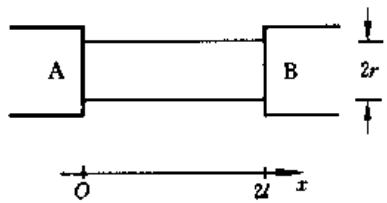
\includegraphics[width=0.3\textwidth]{figures/热图3-26-1.jpg}
\end{center}
\vfill


\newpage
\textbf{3-27} 沿 $x$ 轴在 $x = 0$ 到 $x = L$ 之间放一段长为 $L$ 截面积为 $S$ 的均匀柱体，它与外界绝热。 $t = 0$ 时， $x = 0$ 处的温度为 $T_{1}, x = L$ 处的温度为 $T_{2}$ ，且 $T_{1} > T_{2}$ ，其间温度 $T$ 线性地分布。设柱体的热传导率 $k$ ，比热 $c$ 及密度 $\rho$ 均为常量，各处的热膨胀均可略。试导出 $t$ 时刻 $x$ 处温度 $T(x, t)$ 的积分表达式。
\vfill

\textbf{3-28} 在温度为 $T$ 的恒温热源中有一导热容器，它被隔板分成体积均为 $V$ 的左、右两部分，隔板上有一小孔，面积为 $A$ ，开始时 $(t = 0)$ ，左方装有摩尔质量为 $\mu_{1}$ 的 $\nu \mathrm{mol}$ 理想气体，右方装有另一种摩尔质量为 $\mu_{2}(\mu_{2} \neq \mu_{1})$ 的 $\nu \mathrm{mol}$ 理想气体。由于孔很小，虽然板两侧不断有分子交换，但仍可假定在任一时刻系统都处于平衡态。

1. 试求隔板左、右两侧气体的密度 $\rho_{L}, \rho_{R}$ 各自随时间 $t$ 的变化关系。

2. 试计算最后达到 $\rho_{L} = \rho_{R}$ 时，气体系统的熵的增量。
\vfill

\newpage
\textbf{3-29} 利用布朗运动的实验可以粗略测量阿伏伽德罗常数 $N_{A}$

作布朗运动的微粒系统可以看作是在计及浮力的重力场中达到平衡态的巨分子系统,其数密度遵循玻尔兹曼分布律．设在某实验中，半径 $r=2.12\times10^{-7}$ m，质量密度 $\rho=1.194\times10^{3}$ kg/m$^{3}$ 的球形布朗粒子，悬浮在密度 $\rho_{0}=1.0\times10^{3}$ kg/m$^{3}$ 、温度 T=273 K 的液体中．在高度相距为 $\Delta h=3.0\times10^{-5}$ m 的两处，测得布朗粒子的数密度之比为 $n_{1}:n_{2}=2.08$ .

试求 $N_{A}$ 。
\vfill
\newpage

\textbf{3-30} 流体中悬浮小颗粒的布朗运动尽管很复杂，但它在不断被碰撞中像一个大分子一样按能量均分定理获得了自己的运动能量，这就为讨论它的位移方均量提供了基础。

为讨论方便, 考虑在 $x$ 方向的一维布朗运动. 小颗粒在 $x$ 方向的碰撞净作用力 $F(t)$ 和阻尼力 $f(t)$ 的作用下运动. 若 $t = 0$ 时刻小颗粒处于 $x = 0$ 位置, 那么可以肯定, 在尔后任何时刻 $t$ 都有 $\overline{x(t)} = 0$ , 但 $\overline{x^2(t)}$ 必不为零. 由于热平衡是动态平衡, $F(t)$ 将在零值左右波动, 但必有 $\overline{F(t)} = 0$ . 设小颗粒是半径为 $R$ 的球体, 它所受流体的粘滞阻力为 $f(t) = -6\pi R\eta v_x$ , 其中 $v_x$ 是小颗粒在 $x$ 方向的运动速度, $\eta$ 是流体的粘滞系数. 设实验中所采用的布朗运动小颗粒的质量 $m \ll 6\pi R\eta$ .

1. 试用牛顿第二定律,证明在温度为 T 时有很好的近似解

$$
\overline{x^2(t)} = \frac{kT}{3\pi R\eta}t
$$

式中 $k$ 为玻尔兹曼常量.

2. 取 $R = 5.0 \times 10^{-6} \mathrm{~m}$ 的细小油珠, 测量它悬浮在氮气中时沿水平方向 $x$ 的布朗运动. 每隔 $5 \mathrm{~s}$ 测量一次油珠的 $x$ 坐标, 每两个相邻的 $x$ 值之差记为 $\Delta x$ . 实验中测出 695 个 $\Delta x$ 值, 按 $\Delta x$ 的大小分为 27 组, 每一组中的 $\Delta x$ 相同, 每一组中 $\Delta x$ 的个数记为 $n$ , 详如下表.
\begin{center}
    \begin{tabular}{|c|c|c|c|c|c|c|c|c|}
    \hline
    $\Delta x/(10^{-6} \mathrm{m})$ & $-13$ & $-12$ & $-11$ & $-10$ & $-9$ & $-8$ & $-7$ & $-6$ \\
    \hline
    $n$ & $0$ & $2$ & $4$ & $5$ & $10$ & $14$ & $22$ & $26$ \\
    \hline
    $\Delta x/(10^{-6} \mathrm{m})$ & $-5$ & $-4$ & $-3$ & $-2$ & $-1$ & $0$ & $1$ & $2$ \\
    \hline
    $n$ & $29$ & $35$ & $45$ & $49$ & $63$ & $75$ & $60$ & $54$ \\
    \hline
    $\Delta x/(10^{-6} \mathrm{m})$ & $3$ & $4$ & $5$ & $6$ & $7$ & $8$ & $9$ & $10$ \\
    \hline
    $n$ & $45$ & $37$ & $31$ & $27$ & $20$ & $16$ & $9$ & $8$ \\
    \hline
    $\Delta x/(10^{-6} \mathrm{m})$ & $11$ & $12$ & $13$ & & & & & \\
    \hline
    $n$ & $6$ & $3$ & $0$ & & & & & \\
    \hline
    \end{tabular}
\end{center}
实验是在 $15^{\circ}$ C 下进行的，此时氮气的粘滞系数 $\eta=1.73\times10^{-5}$ Pa·s.

试计算玻尔兹曼常量 k 的值。
\vfill




\chapter{范德瓦耳斯气体、液体、固体、相变}
\newpage
\textbf{4-1} 试求 $1\mathrm{mol}$ 范德瓦耳斯气体由温度 $T_{1}$ ，体积 $V_{1}$ 自由膨胀到体积 $V_{2}$ 时熵的增量，设气体的 $C_V, a, b$ 均为已知的常量。
\vfill

\textbf{4-2} 1 mol氧气在节流过程中体积由高压一边的 $4.0 \times 10^{-3} \, \mathrm{m}^{3}$ 增大到低压一边的 $1.2 \times 10^{-2} \, \mathrm{m}^{3}$ 。已知氧气为范德瓦耳斯气体，范氏常量为 $a = 0.138 \, \mathrm{N \cdot m^{4}/mol^{2}}, b = 3.2 \times 10^{-5} \, \mathrm{m}^{3}/\mathrm{mol}$ ，摩尔定体热容量恒定，为 $C_{V} = 20.8 \, \mathrm{J/(mol \cdot K)}$ 。试计算节流过程前后氧气的温度变化。
\vfill

\newpage
\textbf{4-3} 一定量的乙醚封装在玻璃管内，一部分呈液态，另一部分呈气态，管内无其他杂质。若管内体积恰好为这些乙醚的临界体积，那么在缓慢加热到临界温度时，因气、液两相不再有差别而使液面消失，这就是临界现象的演示实验。假设1mol乙醚的状态方程为 $\left(p+\frac{a}{V^{2}}\right)(V-b)=RT$ ，即为范德瓦耳斯方程，如热图4-3-1所示。

1.已知乙醚的摩尔临界体积为 $V_{K}$ ，在温度为 $T$，压强为饱和蒸汽压时，气相和液相的摩尔体积为 $V_{g}$ 和 $V_{l}$ 。试确定在该温度时玻璃管中气相和液相各占总体积的百分比 $B_{g}$ 和 $B_{l}$ 。

2.在 $V_{g} \gg V_{l}$ 的条件下，试用 $a, b, T$ 来表述 $V_{l}$ 。

3.若在 $20^{\circ}$C 封装乙醚，那么应取 $B_{l}$ 为何值? 已知乙醚临界点的 $T_{K}=466.95\ \mathrm{K}, p_{K}=34.60\ \mathrm{atm}$ 。

\begin{center}
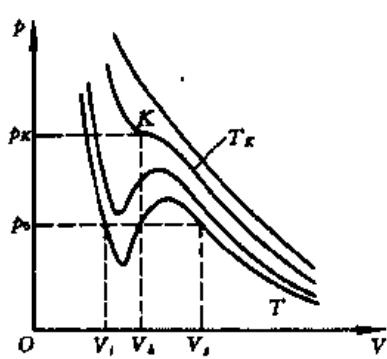
\includegraphics[width=0.2\textwidth]{figures/热图4-3-1.jpg}
\end{center}
\vfill
\newpage

\textbf{4-4} 一种所谓的第二类永动机装置如热图4-4-1所示。图中水平放置的大容器密封但与大气导热，容器左侧A处被围出一个毛细管区域，上方直通容器顶部，右方是实物B，B的外面有相当大的空间 C。图中 D 为一导通管，内有活塞 E 可以无摩擦地左右移动。F 和 G 是两个活门，F 可在一定的压差作用下打开，直到压差几乎为零时才关闭；G 则在一定的压差作用下关闭，直到压差几乎为零时又打开，使 D 与 C 导通。图中水平虚线区域代表某种液体，它与图中所有固体部分均为完全润湿，空白部分只有该液体的饱和蒸汽。

设计者依据：第一，图中用点标出的两处饱和蒸汽压 $p_{1}$ 和 $p_{2}$ 相同。第二，气体内部因高度差引起的附加压强。推证出该装置能往复地从单一热源（大气）吸取热量全部转化为机械功，而不产生其他影响。

1.试完成设计者的推证过程。

2.通过对这个永动机装置的否定，导出 $p_1$ 与 $p_2$ 之间的定量关系，所需参量可自行设取。

\vfill

\newpage
\textbf{4-5} 如热图4-5-1，在一根两端开口、内直径为 $1.0\mathrm{mm}$ 的圆柱形毛细管中，滴入一滴水，然后将它竖直放置。若这滴水在毛细管中分别形成 $1.\, 2.00\mathrm{cm}$，$2.\, 4.00\mathrm{cm}$，$3.\, 2.98\mathrm{cm}$ 的水柱。试问在这三种情况下水柱下端的液面是平面，还是向液体内部凹陷的或向液体外部凸出的曲面？设毛细管能完全润湿水，已知水的表面张力系数 $\alpha = 0.073\mathrm{N / m}$ 。
\begin{center}
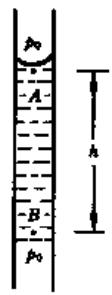
\includegraphics[width=0.08\textwidth]{figures/热图4-5-1.jpg}
\end{center}
\vfill

\textbf{4-6} 如热图4-6-1，有一总长度为 $L$ ，粗细均匀的 $U$ 型毛细管，将它的两个开口端竖直向下稍稍浸入两个容器的等高液面之中。因毛细作用，液体1和液体2分别在毛细管中上升了 $h_1$ 和 $h_2$ 的高度。设液体1和2的密度分别为 $\rho_{1}$ 和 $\rho_{2}$ ，它们与毛细管壁的接触角均为 $0^{\circ}$ ，设液体在毛细管中上升时管内气体无外漏，大气压强为 $p_0$ 。

试求液体1与液体2的表面张力系数的比值。
\begin{center}
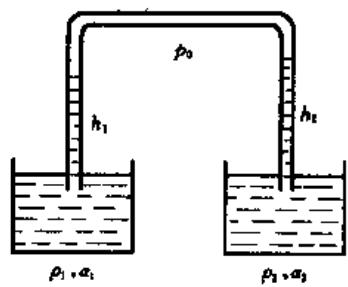
\includegraphics[width=0.2\textwidth]{figures/热图4-6-1.jpg}
\end{center}
\vfill

\newpage
\textbf{4-7} 已知水在1 atm和4 ℃时的表面张力系数 $\alpha = 7.24 \times 10^{-2} \, \mathrm{N/m}$ ，等温压缩系数 $\beta = -\frac{1}{V} \left( \frac{\partial V}{\partial p} \right)_T = 4.75 \times 10^{-5} \, \mathrm{atm}^{-1}$ 。若在1 atm和4 ℃时，水平液面下附近水的密度为 $\rho_0$ 。试问在1 atm和4 ℃时，半径 $r = 1.0 \times 10^{-6} \, \mathrm{cm}$ 的小水滴密度为多大？
\vfill

\textbf{4-8} 在连通管的两端吹出两个相同的球形肥皂泡A和B后，如热图4-8-1，关闭活栓K，活栓 $\mathbf{K}_{\mathrm{A}}$ 和 $\mathbf{K}_{\mathrm{B}}$ 则依旧打开，两泡内的空气经管相通，两泡相对平衡。

1.如热图 4-8-2，若 A 泡和 B 泡的形状小于半球，试证明 A 泡和 B 泡之间的平衡是稳定的。如热图4-8-3，若A泡和B泡的形状大于半球，试证明A泡和B泡之间的平衡是不稳定的。

2.若 A 泡和 B 泡的形状大于半球，设两管口的半径均为 $r_{1}=2.00\ \mathrm{cm}$ ，A 泡和 B 泡的半径均为 $r_{2}=2.50\ \mathrm{cm}$ 。试问当 A 泡和 B 泡分别变化成何种形状时，两泡能再次达到平衡。设空气因压缩或膨胀所引起的密度变化可以忽略。

\begin{center}
    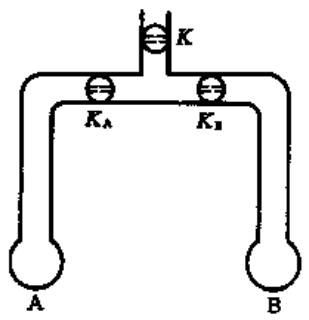
\includegraphics[width=0.1\textwidth]{figures/热图4-8-1.jpg}
    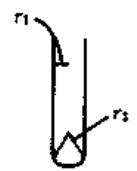
\includegraphics[width=0.1\textwidth]{figures/热图4-8-2.jpg}
    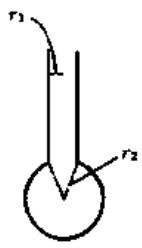
\includegraphics[width=0.1\textwidth]{figures/热图4-8-3.jpg}
\end{center}

\vfill

\newpage
\textbf{4-9} 如热图4-9-1，半径为 $R$ ，密度为 $\rho$ 的匀质球浮在 $0^{\circ}\mathrm{C}$ 的某液体表面上，球心高出液面 $h$。设球的热膨胀可以忽略。已知液体的热膨胀系数为 $\alpha$ ，表面张力系数 $\sigma$ 随摄氏温度 $t$ 的变化关系为 $\sigma(t) = \sigma_0(1 - \beta t)$ ，其中 $\beta$ 为常量。设液体对球为完全润湿。试证明，当系统温度小幅度变化时，球浸入液体部分体积不变的条件为
$$
\frac {\beta - \alpha}{\alpha} = \frac {2 R ^ {4} \rho g}{3 \sigma_ {0} (R ^ {2} - h ^ {2})}
$$
\begin{center}
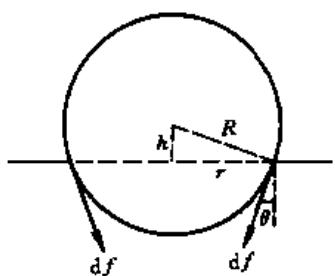
\includegraphics[width=0.2\textwidth]{figures/热图4-9-1.jpg}
\end{center}
\vfill

\textbf{4-10} 同一液体的两个球形膜碰在一起后，形成如热图4-10-1所示的对称连体膜。连体膜的两个球面（实际上是两个超过半球面的部分球面）的半径均为 $R$ ，中间相连的圆膜的半径为 $r$ ，圆膜边缘用一匀质细线围住。已知液体的表面张力系数为 $\sigma$ ，不计重力。试求细线内的张力 $T$ 。
\begin{center}
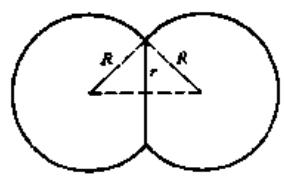
\includegraphics[width=0.2\textwidth]{figures/热图4-10-1.jpg}
\end{center}
\vfill

\newpage
\textbf{4-11} 将一竖直无限大平板部分地浸入与其有润湿作用的液体之中，两者之间的接触角为 $\theta$，液体密度为 $\rho$ ，表面张力系数为 $\alpha$ 。试求液体沿此板上升的高度。
\vfill

\textbf{4-12} 由同种原子组成的均匀一维晶体中，只有最相邻的原子之间有相互作用（余皆可略），作用势为 $V(x) = -\frac{A}{x^6} + \frac{B}{x^{12}}$ ，其中 $x$ 是相邻原子的间距， $A$ 和 $B$ 是两个常量。

1.试求平衡时原子间的平均距离。

2.当此晶体在平衡位置附近的相对形变为单位值时，试求其弹性倔强系数（用 A 和 B 表示）。

3.将晶体慢慢拉伸，试问当形变为多大时，晶体会被拉断。

\vfill

\newpage
\textbf{4-13} NaCl晶体在平衡态时 $\mathrm{Na}^{+}$ 和最邻近的 $\mathrm{Cl}^{-}$ 之间的距离为 $r_0 = 2.81\times 10^{-10}\mathrm{m}$ ，绝热压缩系数为 $k_{s} = -\frac{1}{V}\left(\frac{\mathrm{d}V}{\mathrm{d}p}\right)_{s} = 3.3\times 10^{-11}\mathrm{m}^{2} / \mathrm{N}$ ，马德隆常量为 $\alpha = 1.75$ 。试求平衡态时 $1\mathrm{mol}$ NaCl晶体的结合能 $E_{\mathrm{P0}}$ 。
\vfill

\textbf{4-14} 质量为 $2.0\mathrm{kg}$ ，温度为 $-13^{\circ}\mathrm{C}$ ，体积为 $0.19\mathrm{m}^{3}$ 的氟利昂（其分子量为121），在保持温度不变的条件下被压缩，体积减小为 $0.10\mathrm{m}^{3}$ 。试问在此过程中有多少千克的氟利昂被液化。已知在 $-13^{\circ}\mathrm{C}$ 时，液态氟利昂的密度为 $\rho = 1.44\times 10^{3}\mathrm{kg / m}^{3}$ ，饱和蒸汽压为 $p_{\text{饱}} = 2.08\times 10^{5}\mathrm{Pa}$ ，又氟利昂的饱和蒸汽可近似看作理想气体。
\vfill

\newpage
\textbf{4-15} 液体 $A, B$ 互不相溶，它们的饱和蒸汽压 $p$ 与温度 $T$ （绝对温标）的关系为
$$
\ln {\frac {p _ {i}}{p _ {0}}} = {\frac {a _ {i}}{T}} + b _ {i}, \quad i = A \text{ 或 } B
$$
其中 $p_0$ 是标准大气压， $a, b$ 是由液体本身性质确定的常量。测出两个温度的 $\frac{p_i}{p_0}$ 值如下：
$$
4 0 ^{\circ} \mathrm{C}, \quad \frac {p _ {A}}{p _ {0}} = 0. 2 8 4, \quad \frac {p _ {B}}{p _ {0}} = 0. 0 7 2 7 8
$$
$$
9 0 ^{\circ} \mathrm{C}, \quad \frac {p _ {A}}{p _ {0}} = 1. 4 7 6, \quad \frac {p _ {B}}{p _ {0}} = 0. 6 9 1 8
$$

1.在外部压强为 $p_0$ 时，试分别确定 $A$ 和 $B$ 的沸点。

2.现将 $100\mathrm{g}$ 液体 $A$ 和 $100\mathrm{g}$ 液体 $B$ 先后注入容器内，并在 $B$ 的表面覆盖上一薄层非挥发性液体 $C$，$C$ 与 $A$ 和 $B$ 互不相溶，$C$ 的作用是防止 $B$ 的自由蒸发。如热图4-15-1，各液层都不厚，因此液体内因重力产生的附加压强均可忽略。已知液体 $A$ 和 $B$ 的分子质量之比为 $\gamma = \frac{\mu_A}{\mu_B} = 8$ 。

缓慢而持续地加热容器，液体的温度 $t$ （摄氏温标）随时间 $\tau$ 的变化关系如热图 4-15-2 所示。试求出热图 4-15-2 中的温度 $t_1$ 和 $t_2$ （精确到 1℃），以及在 $\tau_1$ 时刻液体 A 和液体 B 的质量（精确到 0.1 g）。

\begin{center}
    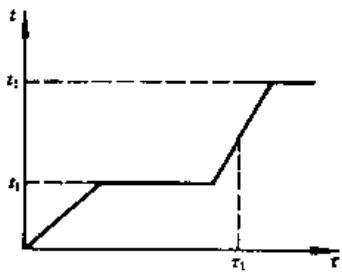
\includegraphics[width=0.3\textwidth]{figures/热图4-15-2.jpg}
    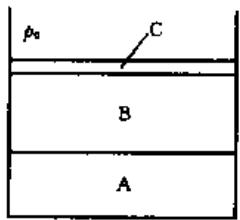
\includegraphics[width=0.3\textwidth]{figures/热图4-15-1.jpg}
\end{center}
设 A 和 B 的蒸汽均可看作理想气体，因而服从道尔顿分压定律。

\vfill
\newpage

\textbf{4-16} 在一密闭容器内有冰、水和水蒸汽各 $1\mathrm{g}$ ，三态共存达到平衡，系统的温度为 $t = 0.01$ ℃，压强为 $p = 4.58 \, \mathrm{mmHg}$ ，容器内别无其他物质。现在保持容器体积不变的条件下，对此系统缓慢加热，输入热量 $Q = 0.255 \, \mathrm{kJ}$ 。试估算此系统再次达到平衡后，冰、水和水蒸汽各自的质量。已知冰的升华热 $L_{\text{升}} = 2.83 \, \mathrm{kJ/g}$ ，水的汽化热 $L_{\text{汽}} = 2.49 \, \mathrm{kJ/g}$ 。
\vfill


\textbf{4-17} 地球深处 $35\mathrm{km}$ 到 $2900\mathrm{km}$ 之间的区域为固态地幔，地幔的主要成分是固态硅酸盐。设硅酸盐的熔解热为 $L_{m}$ ，其液态密度与固态密度之比为 $\alpha$ 。试求地幔中硅酸盐岩石的熔点 $T_{m}$ 随 $r$ 的变化率， $r$ 是岩石与地心的距离。

若已知地幔较上部位某处的 $T_{m}=1300\;^{\circ}\mathrm{C},\alpha=0.9,L_{m}=10^{5}\;\mathrm{cal/kg}$ 。试估算从该处往地心深入1000 m后， $T_{m}$ 变化了多少？
\vfill


% ========== 第三部分 电磁学 ==========
\chapter{静电场、导体与介质}
\newpage
\textbf{1-1} 真空中有两个点电荷 $q_{1}$ 和 $q_{2}$ ，它们的质量分别为 $m_{1}$ 和 $m_{2}$ ，位置矢量分别为 $\pmb{r}_{1}$ 和 $\pmb{r}_{2}$ ，只考虑其间的库仑相互作用。

1. 引入相对位矢 $r = r_2 - r_1$ ，试建立 $r(t)$ 的微分方程。

2. 设 $t = 0$ 时刻, 两点电荷均静止, 相互间距为 $\pmb{r}_0$ . 若两点电荷电量异号, 试问它们何时相碰.
\vfill

\textbf{1-2} 如电图1-2-1，在边长为 $a$ 的正方形的四个顶点分别有电量均为 $Q$ 的固定的点电荷。在正方形对角线交点上放置一个质量为 $m$ 、电量为 $q(q$ 与 $Q$ 同号)的自由点电荷。今将 $q$ 沿某一对角线移动一个很小的距离。试问 $q$ 是否将作周期性振动，若是，试求出振动周期。

\begin{center}
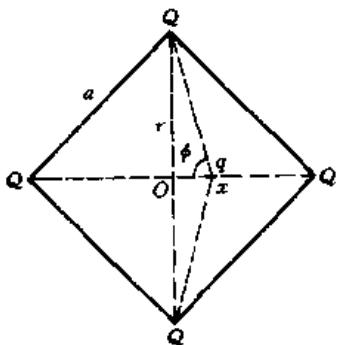
\includegraphics[width=0.2\textwidth]{figures/电图1-2-1.jpg}
\end{center}
\vfill

\newpage
\textbf{1-3} 如电图1-3-1所示，在 $x$ 轴的 $\pm a$ 处分别有两个固定的点电荷，它们的电量均为 $Q(Q > 0)$ 。在 $x$ 轴的 $\pm 2a$ 处分别有另外两个固定的点电荷，它们的电量均为 $-8Q$ 。在原点 $O$ 有一个电量为 $q(q > 0)$ 、质量为 $m$ 的带电质点。设带电质点只能在 $x$ 轴上运动。试分析带电质点所在的平衡位置原点 $O$ ，是否为稳定平衡位置。若原点 $O$ 为稳定平衡位置，将带电质点移到 $x = A$ 处从静止释放 $(0 < A \ll a)$ ，试求其振动周期。
\begin{center}
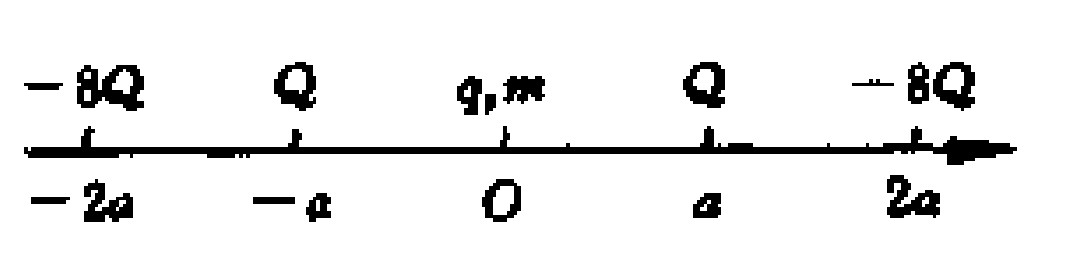
\includegraphics[width=0.2\textwidth]{figures/电图1-3-1.jpg}
\end{center}
\vfill

\textbf{1-4} 电力与距离平方成反比是库仑定律的主要内容。对此，迄今仍有人进行精确的实验检验。试证明，若电力反平方律是精确的，则孤立带电导体球壳达到静电平衡时，其电量将均匀分布在外球面上，球壳内电场强度处处为零。

\vfill

\newpage
\textbf{1-5} 在 $xy$ 平面上有一以坐标原点为圆心，以 $R$ 为半径的带电圆环。电荷线密度的分布为： $y < 0, \lambda = \lambda_0; y > 0, \lambda = -\lambda_0$ 。试求 $z$ 轴（通过圆环的圆心，与圆环所在平面垂直的轴）上的场强分布。
\vfill

\textbf{1-6} 一无限长均匀带电细线弯成如电图1-6-1所示的平面图形，其中AB是半圆弧， $AA'$ 和 $BB'$ 是两平行直线， $A'$ 和 $B'$ 向右端无限延伸．试求圆心O处的电场强度．

\begin{center}
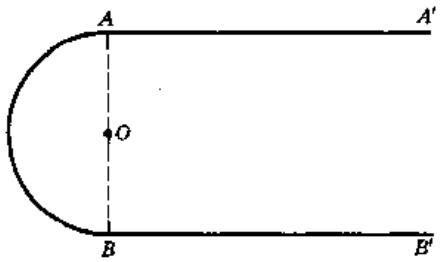
\includegraphics[width=0.25\textwidth]{figures/电图1-6-1.jpg}
\end{center}
\vfill

\newpage
\textbf{1-7} 半径为 $R$ 的半圆环均匀带电，电荷线密度为 $\lambda$ ，试求圆心处的电场强度.
\vfill

\textbf{1-8} 在空间 $A$ 点有电量为 $5Q$ 的固定点电荷，在 $B$ 点有电量为 $12Q$ 的固定点电荷。 $A$ 点和 $B$ 点相距 $13a$ ，空间另一 $C$ 点与 $A$ 点和 $B$ 点分别相距 $5a$ 和 $12a$ 。

1. 以 $C$ 点为球心，以 $r = a$ 为半径作一球。试求在该球区域内，静电场电场强度 $\pmb{E}$ 的平均值

$$
\overline {\boldsymbol {E}} = \frac {\sum_ {i} \boldsymbol {E} _ {i} \Delta V _ {i}}{\sum_ {i} \Delta V _ {i}}
$$

的大小 $|\overline{\boldsymbol{E}}|$ ，式中 $\pmb{E}_i$ 是在体积元 $\Delta V_i$ 处的电场强度。

2. 以 $C$ 点为球心, 以 $r = 10a$ 为半径作一球. 试求在该球区域内, 静电场电场强度 $\pmb{E}$ 的平均值的大小 $|\overline{\pmb{E}}|$ .
\vfill

\newpage
\textbf{1-9} 如电图1-9-1所示，在半径为 $R$ 、体电荷密度为 $\rho$ 的均匀带电球体内部挖去半径为 $R^{\prime}$ 的一个小球, 小球球心 $O'$ 与大球球心 $O$ 相距为 $\alpha$ . 试求 $O'$ 的电场强度, 并证明空腔内电场均匀.

\begin{center}
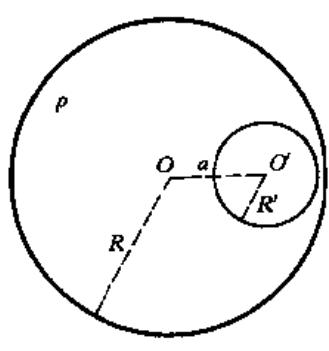
\includegraphics[width=0.2\textwidth]{figures/电图1-9-1.jpg}
\end{center}
\vfill

\textbf{1-10} 如电图1-10-1所示，把半径为 $R$ 的球体切为八等份，取其中一份，使之均匀带电，电荷体密度为 $\rho$ 。试求此八分之一带电球体在球心 $O$ 处的电场强度大小 $E_0$ 。
\begin{center}
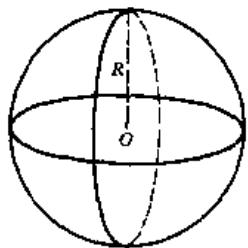
\includegraphics[width=0.2\textwidth]{figures/电图1-10-1.jpg}
\end{center}
\vfill

\newpage
\textbf{1-11} 在惯性系 $S$ 中有匀强电场 $\pmb{E}$ , 其方向如电图1-11-1所示. 在电场中与 $\pmb{E}$ 平行的一条几何直线 (图中画虚线) 上, 有两个静止的小球 A 和 B. 两小球的质量均为 $m$ , A 球所带电量为 $Q(Q > 0)$ , B 球不带电, 开始时两球相距为 $l$ . 在电场的作用下, A 球开始沿直线运动, 并与 B 球发生弹性正碰撞, 从而使 B 球也参与运动. 设在各次碰撞过程中, A 球和 B 球之间并无电量的转移. 设万有引力可略去不计.
\begin{center}
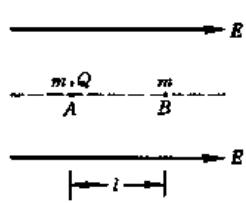
\includegraphics[width=0.2\textwidth]{figures/电图1-11-1.jpg}
\end{center}
试证明，A球与B球相邻两次碰撞之间的时间间隔相同，并求出该时间间隔 $T$
\vfill

\textbf{1-12} 在 $-d \leqslant x \leqslant d$ 的空间区域内，电荷体密度 $\rho > 0$ 为常量。其他区域均为真空。若在 $x = 2d$ 处将质量为 $m$ 、电量为 $q(q < 0)$ 的带电质点自静止释放。试问经多长时间它能到达 $x = 0$ 位置。设带电质点只受电力，其余引力、阻力等均可忽略。
\vfill

\newpage
\textbf{1-13} 在半径为 $R$ 的细圆环上分布着不能移动的正电荷，总电量为 $Q$

1. 如果某个点电荷 $Q_{1} (\neq 0)$ 可在环中指定直径 AOB 线段内作匀速直线运动，试确定圆环上电荷线密度 $\lambda$ 的分布。

2. 取 $x$ 轴沿直径 $AOB$ , 原点 $O$ 在环中心. 将第一问中的点电荷 $Q_{1}$ 放在与 $O$ 点相距 $r_{1}$ 的 $x$ 左半轴上某点. 设电量 $Q_{1}$ 的绝对值为 $Q$ 的 $\nu$ 倍. 能否在 $x$ 右半轴上再放一个非零电量的点电荷 $Q_{2}$ , 使得这两个点电荷及圆环均可保持不动. 设两点电荷都不与环接触, 设环的质量分布均匀. 试求 $Q_{2}$ 及其位置.

3. 把上述两个点电荷 $Q_{1}$ 和 $Q_{2}$ 固定在第二问中确定的位置上, 同时改变它们的电荷符号但保持电量大小不变. 再使环(所带电量 $Q$ 及分布均不变)沿 $x$ 轴的正方向平移一小量 $\delta$ , 然后静止地释放. 试定量讨论环的运动. 设环的质量为 $m$ .

在求解本题时,只需考虑电荷间的库仑作用,其他相互作用均可略.

提示: 把所求的圆环上电荷分布与球面上均匀电荷分布相联系.
\vfill
\newpage

\textbf{1-14} 如电图1-14-1，在半径为 $R$ 、质量为 $m$ 且均匀分布的细圆环上，均匀地分布着总电量为 $q$ 的正电荷。在通过圆环中心 $O$ 点且垂直于圆环平面的 $x$ 轴上有两个固定的点电荷，它们分别在圆环的两侧，与环心的距离均为 $L$ ，各带有电量为 $Q$ 的正电荷.设圆环只能沿 $x$ 轴平动．显然，在上述条件下，圆环处于平衡位置．

\begin{center}
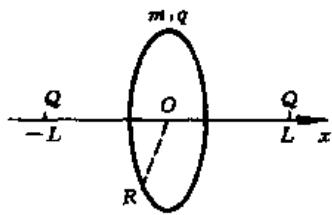
\includegraphics[width=0.25\textwidth]{figures/电图1-14-1.jpg}
\end{center}

1. 试讨论该平衡位置的稳定性(即在什么情况下为稳定平衡位置, 在什么情况下为不稳定平衡位置).

2. 若该位置是稳定平衡位置，试求圆环在其附近作微小振动的周期。
\vfill

\newpage
\textbf{1-15} 如电图 $1 - 15 - 1$ 所示，质量均为 $m$ 、电量均为 $q(q > 0)$ 的一簇带电粒子，从 $P_{1}$ 点以相同速率 $v_{0}$ 在 $xy$ 平面内向右上方各方向射出，即 $\phi$ 角在(0，$\frac{\pi}{2}$ 范围内. 试在 $xy$ 平面内设计一个电场区域, 使这些带电粒子能全部会聚于 $P_{2}$ 点. $P_{1}$ 和 $P_{2}$ 在 $x$ 轴的两侧, 与原点 $O$ 的距离均为 $R$ . 设带电粒子间的相互作用以及引力可略.
\vfill

\textbf{1-16} 如电图1-16-1，两个同心的半球面相对放置，半径分别为 $R_{1}$ 与 $R_{2}(R_{1} > R_{2})$ ，都均匀带电，电荷面密度分别为 $\sigma_{1}$ 与 $\sigma_{2}$ . 试求大的半球底面圆直径AOB上的电势分布.

\begin{center}
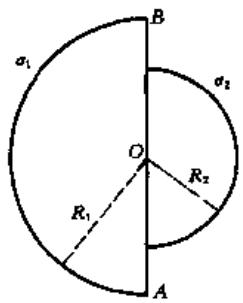
\includegraphics[width=0.15\textwidth]{figures/电图1-16-1.jpg}
\end{center}
\vfill

\newpage
\textbf{1-17} 如电图1-17-1，半径为 $R_{1}$ 的圆环上带有电量 $Q$ ，在它的右边有半径为 $R_{2}$ 的不带电的球面, 球心与环心的间距为 L, 球心与环心的连线和圆环平面垂直. 试求球面上的平均电势 $\overline{U}$ .

\begin{center}
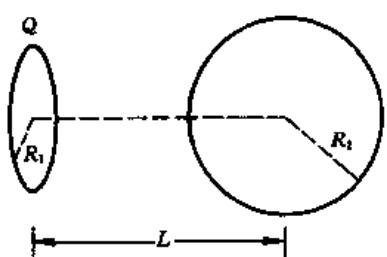
\includegraphics[width=0.25\textwidth]{figures/电图1-17-1.jpg}
\end{center}
\vfill

\textbf{1-18} 地面上有一固定的点电荷A,在A的正上方有一带电小球B,B在重力和A的库仑斥力的作用下,在A上方 $\frac{H}{2}$ 到H之间作往返的自由振动.试求B运动的最大速率 $v_{max}$ .
\vfill

\newpage
\textbf{1-19} 如电图1-19-1所示，两个固定的均匀带电球面A和B分别带电4Q和 $Q(Q>0)$ .两球心之间的距离d远大于两球的半径，两球心的连线MN与两球面的相交处都开有足够小的孔，因小孔而损失的电量可以忽略不计.一带负电的质点静止地放置在A球左侧某处P点，且在MN直线上.设质点从P点释放后刚好能穿越三个小孔，并通过B球球心.试求质点开始时所在的P点与A球球心的距离x应为多少?

\begin{center}
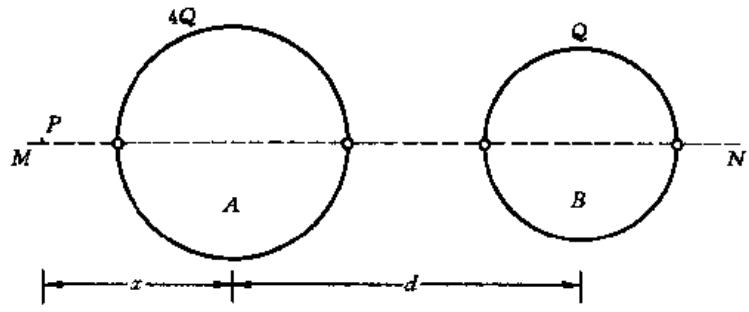
\includegraphics[width=0.3\textwidth]{figures/电图1-19-1.jpg}
\end{center}
\vfill

\textbf{1-20} 半径分别为 $a$ 和 $b$ 的两个同轴无限长半圆柱面如电图1-20-1所示。设在这两个半圆柱面之间有静电场，其电势分布为 $k \ln \frac{b}{r}$ ，其中 $k$ 为某常数， $r$ 是到轴的垂直距离，质量为 $m$ ，电量为 $-q (q > 0)$ 的粒子以初速 $\boldsymbol{v}$ 从图中所示的左方射入， $\boldsymbol{v}$ 既与圆柱面的轴垂直，又与入射处圆柱截面的直径垂直，入射点与轴的距离为 $\rho$ 。

\begin{center}
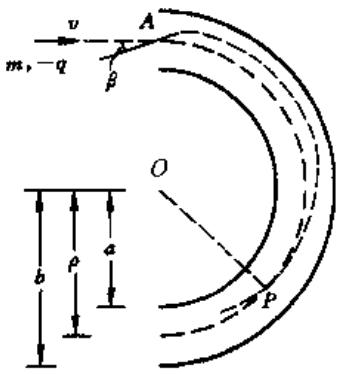
\includegraphics[width=0.15\textwidth]{figures/电图1-20-1.jpg}
\end{center}

1. 试问在什么条件下, 粒子能沿半圆轨道运动.

2. 若入射方向与原设计方向有很小的偏向角 $\beta$ , 如电图1-20-1所示, 那么粒子轨道也将偏离原来的半圆轨道, 设两个轨道的交点为 $P$ . 试证明, 对于很小的偏向角 $\beta, P$ 点的位置与 $\beta$ 无关, 并求出 $P$ 点的方位角 $\angle AOP$ 的大小.
\vfill

\newpage
\textbf{1-21} 在平面上有一段长为 $l$ 的均匀带电直线 $AB$ ，在该平面取直角坐标 $Oxy$ ，原点 $O$ 为 $AB$ 中点， $AB$ 沿 $x$ 轴， $y$ 轴与 $x$ 轴垂直。

1. 试证明, 该平面上任一点 $P$ 的电场强度方向沿 $\angle APB$ 的角平分线.

2. 试求该平面上的电场线方程.

3. 试求该平面上的等势线方程。
\vfill

\textbf{1-22} 如电图1-22-1，在 $x$ 轴的 $-a$ 和 $a$ 两点分别放置电量均为 $Q$ 的点电荷.

试求:1. 在 $xy$ 平面上, 电场强度相对坐标原点 $O$ 为径向的点的轨迹.

2. 在 $xy$ 平面上, 电场强度相对坐标原点 $O$ 为切向的点的轨迹.

(注:所谓径向或切向,均指电场强度 E 的方向相对原点 O 沿径向或切向,并非 E 的径向或切向分量.)

\begin{center}
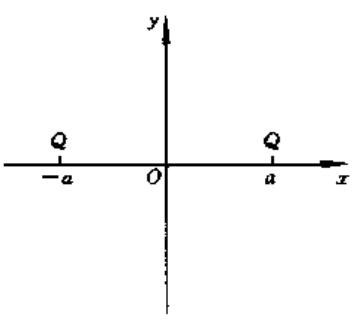
\includegraphics[width=0.25\textwidth]{figures/电图1-22-1.jpg}
\end{center}
\vfill

\newpage
\textbf{1-23} 线电荷密度分别为 $\lambda$ 和 $-\lambda (\lambda =$ 常量）的两平行无限长带电直线相距 $2a$ ，试求等势面和电场线的空间分布．
\vfill

\textbf{1-24} 已知真空中电场的能量密度为 $w_{\mathrm{e}} = \frac{1}{2}\varepsilon_0E^2$ . 试求:

1. 均匀带电球面 (电量为 $Q$ , 半径为 $R$ ) 的球面上的电场强度值. 

2. 带电球面上的表面张力系数 $\sigma$ .
\vfill

\newpage
\textbf{1-25} 有1998个半径相同的导体球，各球均带有相同的正电荷，彼此不接触。试证明，在静电平衡时，至少有一个导体球的表面处处无负电荷。
\vfill

\textbf{1-26} 质子加速器使每个质子得到的动能为 $E$ 。很细的质子束从加速器射向一个远离加速器的半径为 $r$ 的金属球，并留在球上。球的中心并不处在加速器发射出的质子运动方向的直线上，而与该直线的垂直距离为 $d$ ，且 $d < r$ 。试问加速器工作足够长时间后，球能充电到多高的电势？

计算时, 可取 $E = 2 \text{kev}$ 和 $d = \frac{r}{2}$ . 又, 若把质子换成电子, 将会发生什么变化?
\vfill

\newpage
\textbf{1-27} 如电图1-27-1所示，导体球A、B和C的半径分别为 $2\mathrm{cm}, 2\mathrm{cm}$ 和 $3\mathrm{cm}$ ，它们的球心构成边长为 50 cm 的等边三角形 ABC. 开始时, A、B、C 三球各带电荷 $12 \times 10^{-9}$ C、 $24 \times 10^{-9}$ C、 $30 \times 10^{-9}$ C, 试求 B 球电势的近似值, 并估算所用近似方法产生的误差.

若将三球用导线彼此相连,忽略连接后导线上的电荷分布,试求各球所带电量.

设 Ox 轴通过 $\triangle ABC$ 的中心，并垂直于 $\triangle ABC$ 所在平面。试计算导线将三球连接后，在 Ox 轴上与 O 点的距离等于 CO 的那一点的电场强度。

\begin{center}
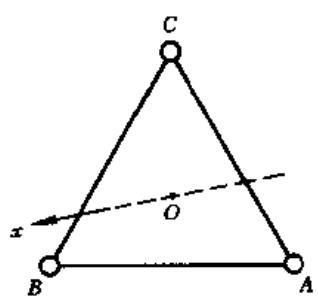
\includegraphics[width=0.15\textwidth]{figures/电图1-27-1.jpg}
\end{center}
\vfill

\textbf{1-28} 如电图1-28-1所示，在真空中有四个半径均为 $a$ 的不带电的相同导体球，球心分别位于边长为 $r$ 的正方形的四个顶点之上， $r \gg a$ 。现让球1带 $Q$ 的电荷 $(Q > 0)$ ，然后取一细金属丝, 它的一端固定在球 1 上, 另一端分别依次与球 2、3、4 接触. 设每次接触的时间都足够长, 使它们达到静电平衡后, 再断开. 设分布在细金属丝上的电荷可忽略不计. 试求四小球最后所带电量 $Q_{1}, Q_{2}, Q_{3}, Q_{4}$ .

\begin{center}
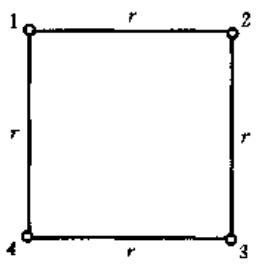
\includegraphics[width=0.15\textwidth]{figures/电图1-28-1.jpg}
\end{center}
\vfill

\newpage
\textbf{1-29} 如电图1-29-1所示,三根等长的带电绝缘细棒首尾相接构成三角形,其中电荷的分布如同绝缘棒都换成等长导体棒且已达到静电平衡时的电荷分布。测得图中 $A$ 点和 $B$ 点的电势分别为 $U_{A}$ 和 $U_{B}$ 。假设若将 $ab$ 棒取走，并不影响 $ac$ 及 $bc$ 两棒的电荷分布。试求此时 $A$ 点和 $B$ 点的电势。

\begin{center}
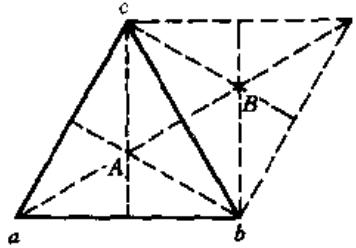
\includegraphics[width=0.2\textwidth]{figures/电图1-29-1.jpg}
\end{center}
\vfill

\textbf{1-30} 如电图 $1 - 30 - 1$ 所示，恒温的矩形盒内装有理想气体，当隔板将盒等分为二时，两侧气体压强均为 $P_{0}$ 。当隔板平行移动时，无摩擦，不漏气，两侧气体经历准静态过程。隔板是面积为 $A$ 的金属板，带电量为 $Q$ ，矩形盒上与它平行的两块板也是金属板，面积也为 $A$ ，相距为 $2L$ ，固定，并接地。隔板两侧的电场均匀。盒的其余部分是不导电的绝缘板。

1. 试求隔板的平衡位置。

2. 试讨论平衡是否稳定。
\begin{center}
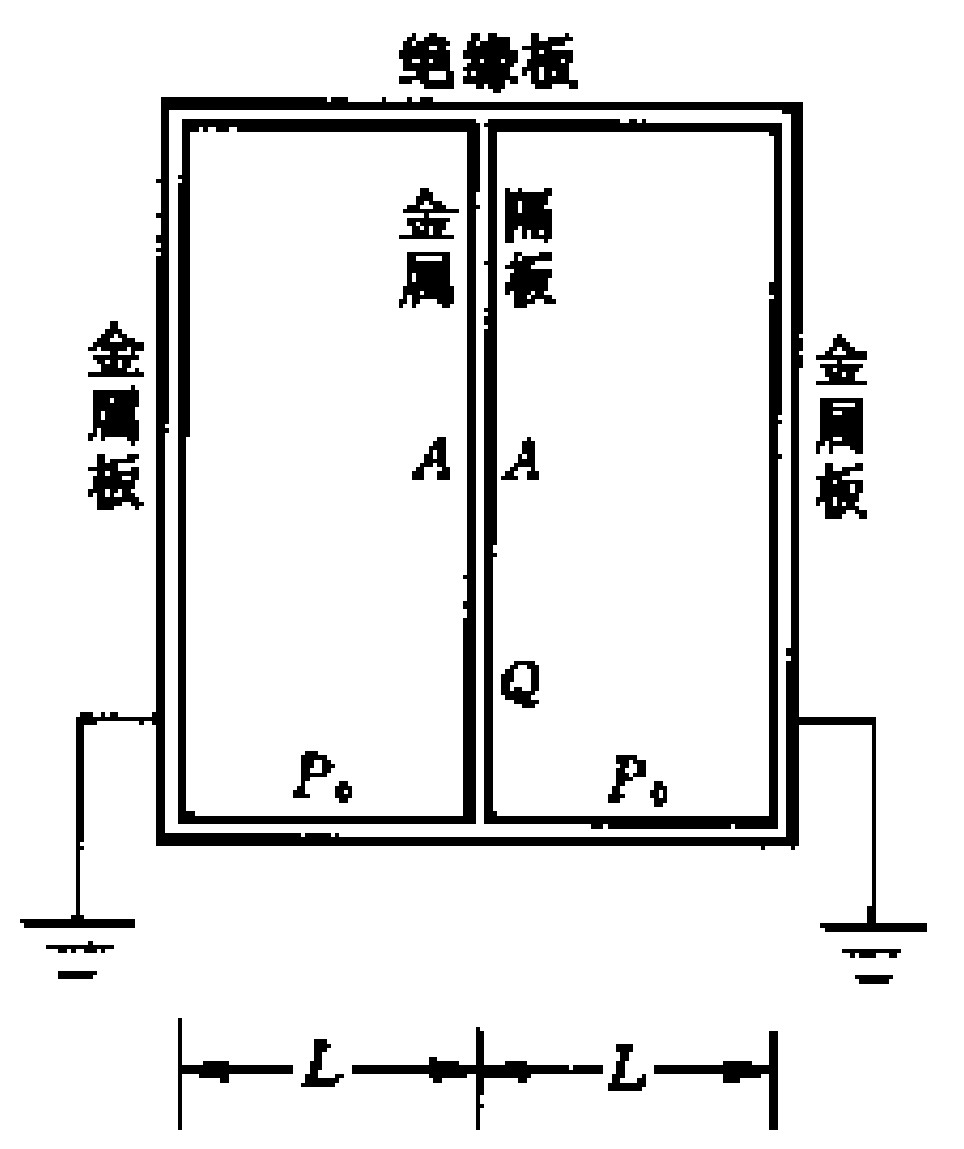
\includegraphics[width=0.1\textwidth]{figures/电图1-30-1.jpg}
\end{center}
\vfill

\newpage
\textbf{1-31} 如电图1-31-1所示，在半径为 $R$ 的接地金属圆柱面的中央放有一根半径为 $r_0$ 的同轴细长导线，导线处于正的高电势 $U_0$ 。于是导线外侧附近介质原子被电离成自由电子与正离子，其中自由电子即被导线吸附,正离子则离开导线径向地运动.设正离子的径向迁移率(径向速度与电场强度的比值)为常数w,且迁移过程中正离子始终围绕导线形成均匀的圆柱形薄层.

\begin{center}
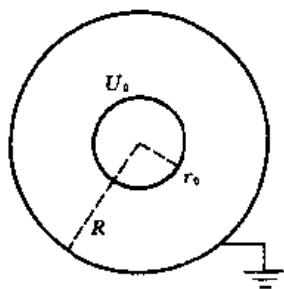
\includegraphics[width=0.3\textwidth]{figures/电图1-31-1.jpg}
\end{center}

1. 试证明,作为时间 $t$ (从正离子在导线外侧附近形成的时刻开始计时)的函数,正离子的径向位置 $\boldsymbol{r}$ 可表为
$$
r ^ {2} = k (t + t _ {0})
$$
并求出常量 k 和 $t_{0}$ (略去由于介质电离造成的电场变化).

2. 设全部正离子电量为 Q，为了使导线电势保持原来的 $U_{0}$ 不变，需给导线补充电量 $Q^{*}$ . 试导出 $Q^{*}$ 与时间 t 的关系.
\vfill

\textbf{1-32} 圆形导体薄板的半径为 $R$ ，在其中轴线上与圆板中心 $O$ 相距为 $a$ 处有一个静止的点电荷 $Q$ .设 $a\ll R$ ，忽略边缘效应.

1. 导体板接地，试求导体板上的电荷分布。

2. 导体板不接地, 带有电量 $Q_{0}$ , 试求导体板上的电荷分布.
\vfill

\newpage
\textbf{1-33} 如电图1-33-1所示，两块足够大的接地导体平面A和B平行竖直放置，相距 $2d$ ， $d = 10\mathrm{cm}$ .在两板之间的中央位置，用长 $l = 1\mathrm{m}$ 的绝缘细线悬挂一个质量 $m = 0.1\mathrm{g}$ ，电量 $q = 5\times 10^{-9}\mathrm{C}$ 的小摆球．让小摆球稍稍偏离平衡位置后释放，使之小角度摆动．忽略各种电磁阻尼和空气阻尼．试求小球的摆动周期 $T$

\begin{center}
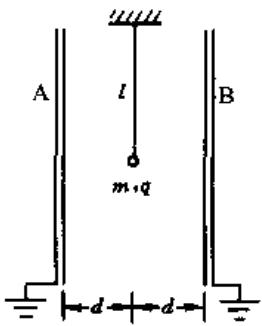
\includegraphics[width=0.2\textwidth]{figures/电图1-33-1.jpg}
\end{center}
\vfill

\textbf{1-34} 半径为 $R$ 的导体球带有电量 $Q(Q > 0)$ 。今在距球心为 $a$ 处 $(a > R)$ 放置一个与 $Q$ 同号的点电荷 $q$ 。为使导体球在静电平衡时受到 $q$ 的作用力吸引，试确定 $q$ 的取值范围。
\vfill

\newpage
\textbf{1-35} 两个半径均为 $R$ 的导体球相互接触形成一孤立导体，试求此孤立导体的电容。
\vfill

\textbf{1-36} 在空间 $n$ 个点上依次放置 $n$ 个点电荷 $q_{1}, q_{2}, \cdots, q_{n}$ , 这些电荷在这 $n$ 个点上产生的总电势分别记为 $U_{1}, U_{2}, \cdots, U_{n}$ . 若在这 $n$ 个点上换成另一组点电荷 $q_{1}^{\prime}, q_{2}^{\prime}, \cdots, q_{n}^{\prime}$ , 则相应的总电势为 $U_{1}^{\prime}, U_{2}^{\prime}, \cdots, U_{n}^{\prime}$ . 试证明
$$
\sum_ {i = 1} ^ {n} q _ {i} U _ {i} ^ {\prime} = \sum_ {i = 1} ^ {n} q _ {i} ^ {\prime} U _ {i}, \quad n \geqslant 2
$$
由此进一步证明, 真空中由一对导体构成的电容器的电容与这两个导体的带电量多少无关.
\vfill

\newpage
\textbf{1-37} 如电图1-37-1所示，A和B是两块相同的水平平行金属板，相距为 $d$ ，构成电容为 $C$ 的平行板电容器.B板接地，B板中有一个小孔，开始时A和B均不带电.在B板小孔上方 $h$ 处，不断有带电小液珠从静止开始自由下落(空气阻力可略)，每个液珠的电量为 $q$ ，质量为 $m$ ，液珠经小孔到达A板后被吸收，液珠的下落保持一定的间隙，即在前一液珠被A板吸收并达到静电平衡后，后一液珠才继续下落．试问有多少个液珠能落到A板上.

\begin{center}
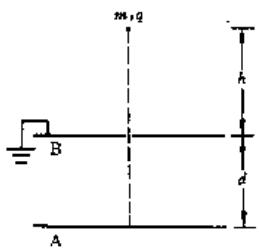
\includegraphics[width=0.2\textwidth]{figures/电图1-37-1.jpg}
\end{center}
\vfill

\textbf{1-38} 如电图1-38-1所示,两个相同的水平放置的平板空气电容器连接起来,充电后电容器A中的带电微粒P刚好静止地悬浮着.撤去电源,将电容器B的两板水平地错开,使两板相对的面积减小为原来的一半.试求此时带电微粒P在竖直方向运动的加速度.

\begin{center}
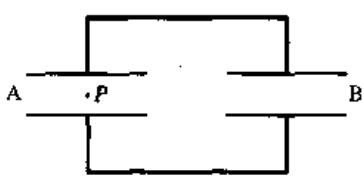
\includegraphics[width=0.2\textwidth]{figures/电图1-38-1.jpg}
\end{center}
\vfill

\newpage
\textbf{1-39} 如电图1-39-1所示，一个边长为 $L$ 的正方形平板电容器，板面竖直地串联在线路中.线路中的直流电源确保电压稳定，为 $V_{0},\mathbf{G}$ 是电流计．一块矩形金属板，垂直于图面方向的长度也为 $L$ ，高为 $L^{\prime}(L^{\prime}\ll L)$ ，厚为 $\frac{D}{P} (D$ 是电容器两板的间距， $P\gg 1$ 是一个系数).开始时，金属板竖直地放在电容器中线(在电图1-39-1中用虚线表示)的正上方，其下端与电容器两板的上端对齐，然后自由落下．忽略各种边缘效应，忽略电磁力对金属板的作用．

试求电容器极板上的电量 Q 随时间 t 的变化关系，并画出流过电流计的电流 I 随时间 t 的变化图线（如电图 1-39-1，设从上到下流过电流计的电流为正，反之为负）.

\begin{center}
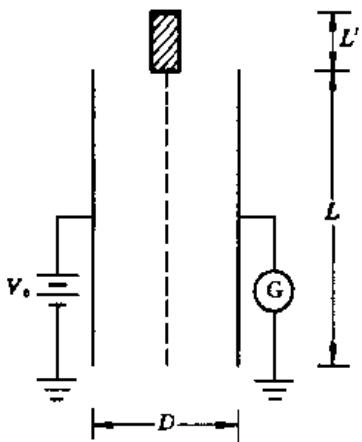
\includegraphics[width=0.15\textwidth]{figures/电图1-39-1.jpg}
\end{center}
\vfill
\newpage

\textbf{1-40} 由直流电源、电容、电阻和开关 K 构成的网络如电图1-40-1所示，其中电源的电动势为 E，三个电容器 $C_{1}$ 、 $C_{2}$ 、 $C_{3}$ 的电容均为 C，两个电阻器的电阻分别为 $R_{1}$ 和 $R_{2}$ 。开始时，三个电容器均不带电，先接通 Oa，再接通 Ob，再换接 Oa，再换接 Ob，…，如此反复换向。设每次换接前都已达到静电平衡。
\begin{center}
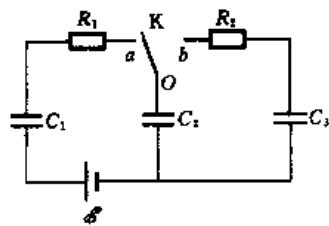
\includegraphics[width=0.25\textwidth]{figures/电图1-40-1.jpg}
\end{center}
试求:1. 第 n 次接通 Ob 并达到静电平衡后, 各电容器两端的电压分别是多少? 2. 当反复换向无穷多次后, 在所有电阻上消耗的总电能是多少?
\vfill

\newpage
\textbf{1-41} 两块长与宽均为 $a$ 与 $b$ 的导体平板在制成平行板电容器时稍有偏斜，使两板一对宽边相距为 $d$ ，另一对宽边相距为 $(d + h)$ ，且 $h \ll d$ 。若此电容器内充满了相对电容率为 $\varepsilon_r$ 的电介质。试求电容器的电容。
\vfill

\textbf{1-42} 如电图1-42-1，两个同轴导体圆筒，内筒半径为 $R$ ，两筒间距为 $d$ ，简高为 $L$ ，且 $L \gg R \gg d$ 。内筒外筒与电源的负极连接．圆筒的中央轴在铅垂线上，筒间 A 和 B 两点的连线与中央轴平行，A 点和 B 点的间距为 h．一个质量为 m，电量为 $-Q(Q>0)$ 的带电粒子从 A 点射出，其速率为 $v_{0}$ ，速度的方向垂直于由 A 点和筒中央轴线确定的平面．为了使该带电粒子能经过 B 点，试求所有可供选择的 $v_{0}$ 和 $C_{x}$ 值．

\begin{center}
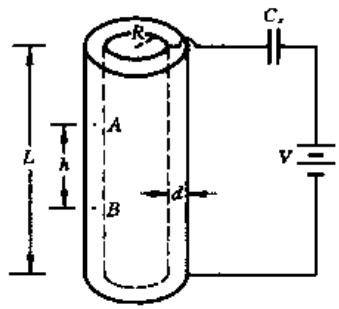
\includegraphics[width=0.2\textwidth]{figures/电图1-42-1.jpg}
\end{center}
\vfill

\newpage
\textbf{1-43} 如电图1-43-1所示，金属球壳上方与一个带有两个活栓的细长玻璃管连接，管壁外包着金属箔，金属箔与电池组的接地端连通，管上方槽中的水银则与电池组另一端正极连通，开始时，球内无水银且不带电，玻璃管下端的活栓关闭，上端的活栓打开，管内充满水银，然后，关闭上端活栓，移开金属箔，再打开下端活栓，使管内水银注入球内。不断重复此过程，直至球内充满水银为止。设电池组的端电压为 $V$ ，玻璃的相对电容率（又称介电常量）为 $\varepsilon_r$ ，管半径为 $r$ ，管壁厚度为 $d$ ，球半径为 $R$ ，且有 $R \gg r \gg d$ 。试近似计算金属球壳充满水银后相对于地的电势。
\begin{center}
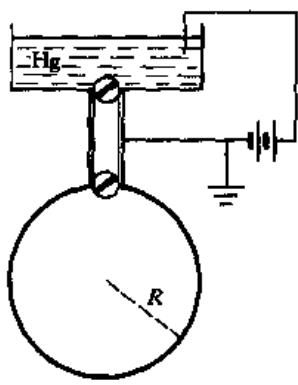
\includegraphics[width=0.2\textwidth]{figures/电图1-43-1.jpg}
\end{center}
\vfill



\chapter{磁场磁介质}
\newpage
\textbf{2-1} 如电图2-1-1所示，电流强度为 $2I$ 的直流电经半无限长导线到达半径为 $R$ 的金属球面的南极点，由球面流到北极点后，再从另一半无限长直导线流向远处。设想将上述电流分布切成左、右两半。左半部分为半无限长直电流 $I$ 到达半球面南极点后，经左半球面（注意，此半球面的电流分布与原全球面左半的电流分布相同）流向北极点，再经半无限长直导线流向远处，并设置 $O - xyz$ 坐标，如图2-1-2所示。试求球心 $O$ 处的磁感应强度 $\pmb{B}$

\begin{center}
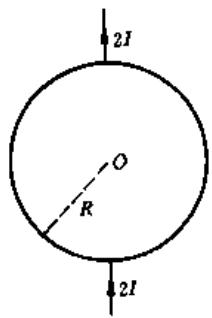
\includegraphics[width=0.15\textwidth]{figures/电图2-1-1.jpg}
\qquad
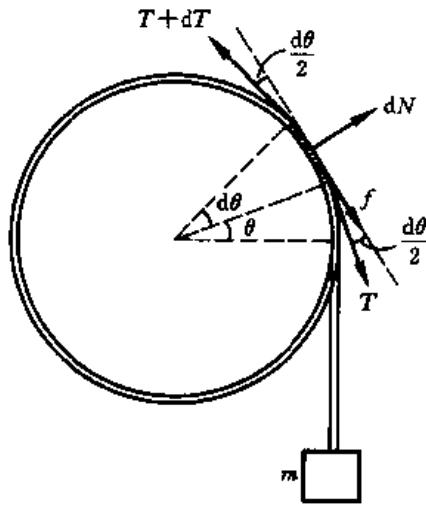
\includegraphics[width=0.2\textwidth]{figures/图2-1-2.jpg}
\end{center}
\vfill

\textbf{2-2} 抛物线形状的无穷长导线载有电流 $I$ 。设焦点到顶点的距离为 $a$ 。试求焦点处的磁感应强度 $B$ 。
\vfill

\newpage
\textbf{2-3} 均匀带电的球面绕着它的某一直径匀速旋转．试证明在该直径上的磁感应强度处处相同．
\vfill

\textbf{2-4} 如电图2-4-1所示，在Oxyz坐标系中有一半径为R的无限长圆柱面，圆柱面的中央轴线沿y轴，圆柱面上绕有螺距为H的无限长等距螺旋导线，导线与x轴相交，导线内通有稳恒电流I.设空间各处的相对磁导率近似为1，试求坐标原点O处的磁感应强度B的三个直角坐标分量 $B_{x},B_{y}$ 和 $B_{z}$ .

\begin{center}
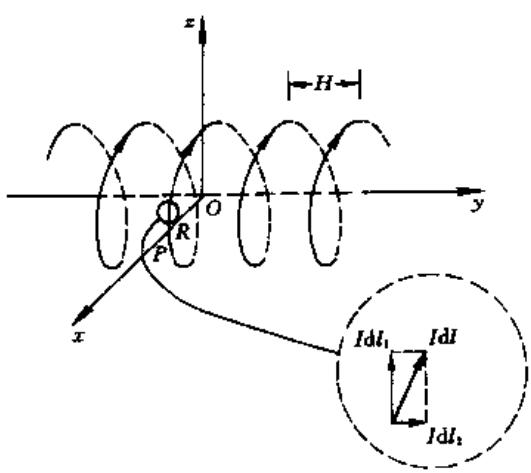
\includegraphics[width=0.3\textwidth]{figures/电图2-4-1.jpg}
\end{center}
\vfill

\newpage
\textbf{2-5} 如电图2-5-1， $C_{+}$ 和 $C_{-}$ 是沿 z 轴放置的两根互相绝缘的长直非磁性导体，其中的电流分别沿 z 轴的正方向和负方向流动, 电流强度均为 $I$ 。图中画斜线的部分是两导体的正截面, 它们分别是 $xy$ 平面中的部分圆, 两圆的直径均为 $D$ , 两圆心的间距为 $\frac{D}{2}$ , 不难算出, 两导体正截面的面积均为 $\left(\frac{1}{12}\pi + \frac{1}{8}\sqrt{3}\right) D^2$ 。每一根导体中的电流均匀地分布在自身的正截面内。 试求两根导体之间空白区域内的磁场分布 $B(x, y)$ 。

\begin{center}
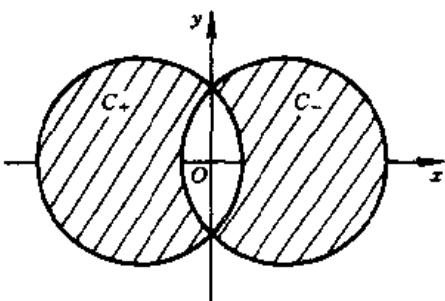
\includegraphics[width=0.25\textwidth]{figures/电图2-5-1.jpg}
\end{center}
\vfill

\textbf{2-6} 如电图2-6-1所示，取直角坐标系 $xyz$ ，在 $-d\leqslant x\leqslant d$ 的一层无穷区域内有均匀的传导电流，电流密度的方向为 $z$ 轴的正方向，大小恒定为 $j$ 试求真空中磁感应强度 $\pmb{B}$ 的分布。

\begin{center}
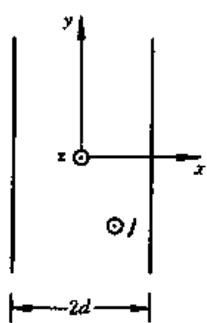
\includegraphics[width=0.25\textwidth]{figures/电图2-6-1.jpg}
\end{center}
\vfill

\newpage
\textbf{2-7} 无限长直圆柱形导体在没有电流时，自由电子的体电荷密度为常量 $\rho_0$ ，正离子的体电荷密度为 $-\rho_0$ ，导体内处于电中性。当沿导体长度方向通以直流电时，体电流会在导体中产生轴对称的环状分布磁场，沿轴向运动的自由电子便会在磁场力的作用下向中轴移动，从而破坏了原来的 $\rho_0$ 分布。当积聚的净电荷产生的径向电场与运动自由电子所受的磁场力恰好抵消时，便形成只沿导体长度方向的稳恒电流。设此时自由电子的漂移速度为 $\bar{u}$ 。试求导体中净电荷密度的分布。
\vfill  

\textbf{2-8} 如电图2-8-1，在水平面上有一根光滑的刚性细长杆，它可以无摩擦地绕固定的竖直轴旋转，转动惯量为 $I$ 。在杆周围有与转轴平行的匀强磁场 $\pmb{B}$ ，其方向如图所示。把质量为 $m$ ，电量为 $q(q>0)$ 的光滑带电小圆环套在杆上,设环与杆之间无电荷转移。

1. 试问杆连同环的旋转角速度 $\omega$ 取何值时, 环在杆上任何位置均可相对杆静止。

2. 设杆的初始角速度 $\omega_{0}$ 大于第 1 问中的 $\omega$ 值，设开始时环静止于转轴位置，后因受微小扰动，环离开转轴位置沿杆运动。试问环是否可能在到达杆的某一位置后，其径向速度降为零，从而停留在该处相对杆保持静止。

3. 若杆的初始角速度改取第2问中所给初始角速度的 $\alpha$ 倍 $(\alpha > 0)$ . 试问为使圆环的运动轨道保持不变, 应如何改变磁场的大小。

\begin{center}
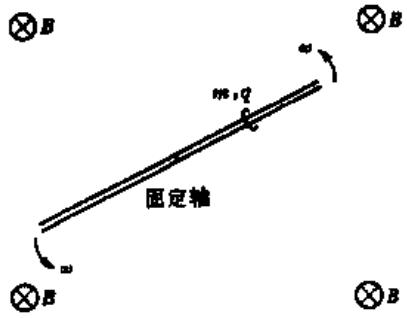
\includegraphics[width=0.2\textwidth]{figures/电图2-8-1.jpg}
\end{center}
\vfill

\newpage
\textbf{2-9} 如电图2-9-1所示，半径为 $R$ ，质量为 $m$ 的匀质细圆环上均匀地分布着相对圆环固定不动的正电荷，总电量为 $Q, t = 0$ 时，圆环在水平地面上具有沿正东方向的平动速度 $\nu_{0}$ ，且无滚动．假设圆环与地面之间的摩擦系数为 $\mu$ ，在圆环周围只有沿水平面指向北方（电图 2-9-1 中垂直纸面向里为北方）的匀强地磁场 B．

1. 为了使圆环在尔后的运动过程中始终不会离开地面，试求 $v_{0}$ 的取值范围。

2. 若 $v_{0}$ 在第一问的取值范围内, 假设圆环最后能达到纯滚状态. 试导出在达到纯滚前, 圆环的平动速度 $v$ 与时间 $t$ 的关系。

3. 设 $v_{0}=\frac{mg}{2QB}$ ，试求圆环则达到纯滚状态的时刻 T.

\begin{center}
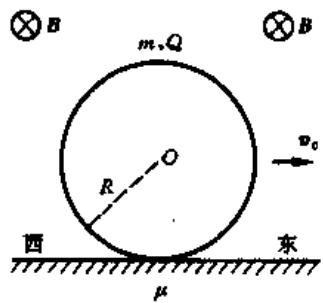
\includegraphics[width=0.2\textwidth]{figures/电图2-9-1.jpg}
\end{center}
\vfill

\textbf{2-10} 如电图2-10-1所示，经 $U = 1000\mathrm{V}$ 电压加速的电子(加速前电子静止)从电子枪T射出，其初速沿直线 $\alpha$ 的方向。若要求电子能击中在 $\varphi = 60^{\circ}$ 方向，与枪口相距 $d = 5.0~\mathrm{cm}$ 的靶M。试求在以下两种情形，所需的匀强磁场的磁感应强度 $\pmb{B}$ 的大小。1. 磁场 $\pmb{B}$ 垂直于直线 $\alpha$ 与靶 M 所确定的平面.2. 磁场 B 平行于枪口 T 向靶 M 所引的直线 TM.

\begin{center}
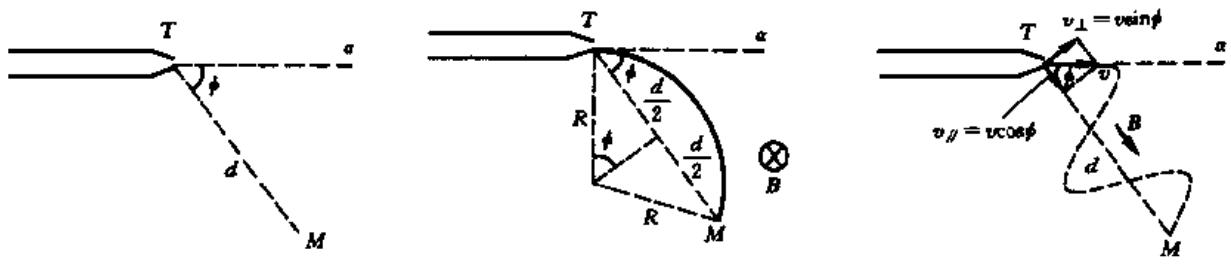
\includegraphics[width=0.6\textwidth]{figures/电图2-10-1.jpg}
\end{center}
\vfill

\newpage
\textbf{2-11} 如电图2-11-1所示，设在本题所涉及的空间范围内有磁感应强度为 $\pmb{B}$ 的匀强磁场，其方向垂直纸平面向里。在纸平面上有一个长为 $h$ 的光滑绝缘空心细管MN，在管的 $M$ 端内有一个质量为 $m$ ，电量为 $q(q > 0)$ 的带电小球 $\mathbf{P}_1$ ，在管的 $N$ 端外侧有另一个不带电的小球 $\mathbf{P}_2$ 。开始时， $\mathbf{P}_1$ 相对管静止，管带着 $\mathbf{P}_1$ 以垂直于管长度方向的速度 $\pmb{u}_{1}$ 在纸面上向图中正右方向运动，小球则以 $\pmb{u}_{2}$ 向着图中正左方向运动。设管的质量远大于 $m$ ，小球 $\mathbf{P}_1$ 在管内运动对管运动的影响可以忽略。设引力可略。如果 $\mathbf{P}_1$ 从管的 $N$ 端离开管后，最终能与 $\mathbf{P}_2$ 相碰。试求满足此要求的 $\pmb{u}_{2}$ 的可能取值。

\begin{center}
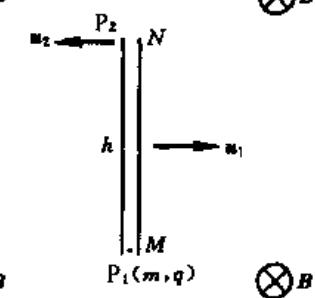
\includegraphics[width=0.2\textwidth]{figures/电图2-11-1.jpg}
\end{center}
\vfill
\newpage

\textbf{2-12} 如电图2-12-1所示，在半径为 $R$ 的圆筒形真空管中有两个隔板，将管内分为三个区域，两隔板中心各有小孔A和 $\mathbf{A}^{\prime}$ ，两孔间距为 $L$ 。在左边的区域I中有加速电场，在中间的区域Ⅱ中有沿管轴方向的匀强磁场 $\pmb{B}$ ，在右边的区域Ⅲ中既无电场也无磁场。区域I中的阴极K连续发射的电子经其中的电场加速后，使穿过小孔A的电子形成发散束进入区域II。设穿过小孔A的这些电子的速度在管轴方向的分量均为 $v$ ，设电子之间的相互作用可以忽略。当将区域Ⅱ中沿管轴方向的磁感应强度的大小调到某些值时，从小孔A进入区域Ⅱ的电子便能穿过小孔 $\mathbf{A}^{\prime}$ 射出，把这些磁场的最小值表为 $B_{0}$ 。取从A到 $\mathbf{A}^{\prime}$ 的方向为正方向，区域Ⅱ中的磁场 $\pmb{B}$ 随时间 $t$ 变化的曲线如电图2-12-2所示。即从 $t = 0$ 起 $\pmb{B}$ 沿正方向，每经 $\frac{T}{2}$ 的时间 $\pmb{B}$ 反向一次， $T$ 就是 $\pmb{B}$ 的变化周期。从 $t = 0$ 开始，电子束连续地从小孔A进入区域Ⅱ，设凡遇管壁的电子均被管壁吸收。

1. 为了使从小孔 A 进入区域 II 的电子能经小孔 A' 到达区域 III, 试求磁场 B 变化周期的最小值 $T_{0}$ .

2. 若取磁场变化周期 $T = 2T_0$ ，试在电图 2-12-2 的时间轴上标明电子能经小孔 A' 到达区域Ⅲ的时间区间。

3. 在进入区域Ⅲ的电子束中, 电子运动方向与管轴之间夹角的最大值是多少?

\begin{center}
\includegraphics[width=0.3\textwidth]{figures/电图2-12-2.jpg}
\quad
\includegraphics[width=0.3\textwidth]{figures/电图2-12-1.jpg}
\end{center}

\vfill

\newpage
\textbf{2-13} 如电图2-13-1所示，一个实心圆柱形导体和一个中空圆柱形导体共轴，其间为真空，内圆柱体的半径为 $a$ ，外圆柱体的内半径为 $b$ 。外圆柱体相对内圆柱体可具有正电势 $V$ ，故称为阳极．在涉及的空间范围内可以存在匀强磁场，磁感应强度 B 的方向与圆柱体的中央轴平行，即垂直于电图 2-13-1 所在的纸平面并外指．设导体的感应电荷一律不予考虑。

本题讨论电子在两圆柱体之间的真空中运动的动力学问题。设电子的静止质量为 m，电量为 -e，电子一律从内圆柱体表面射出。

1.设外圆柱体相对内圆柱体的电势为 $V$ , 设 $B = 0$ . 设有一个电子从内圆柱体表面逸出, 初速可略。试求该电子打到阳极 (外圆柱体) 时的速度大小为 $v$ , 先给出非相对论的答案, 再给出相对论的答案.

以下几问则无需考虑相对论效应。

2.设 $V = 0$ , 设匀强磁场 $\pmb{B}$ 不为零。一个电子以径向初速度 $\nu_0$ 从内圆柱体表面射出, 当磁场超过某一临界值 $B_{\mathrm{C}}$ 时, 电子将不能到达阳极 (外圆柱体), 试求此 $B_{\mathrm{C}}$ 值, 并在磁场略大于 $B_{\mathrm{C}}$ 的情况下, 定性画出电子与内圆柱体相碰前的运动轨道。

3.电子从内圆柱体射出后, 磁场对电子的作用可使电子获得相对圆柱体中央轴的非零角动量 $L$ . 试导出 $L$ 随时间 $t$ 的变化率 $\frac{\mathrm{d}L}{\mathrm{d}t}$ 的表达式。试进而证明, 这一表达式意味着下述量
$$
L - k e B r ^ {2}
$$
是一个不随电子运动而变化的守恒量．其中 k 是一个无量纲的常量，r 是从圆柱体中央轴到电子所在位置的矢径．最后，试确定 k 的值．

4.设一个电子无初速地从内圆柱体表面逸出后不能到达阳极，则它与圆柱体中央轴的距离必定会达到某个相应的极大值 $r_{\max}$ 。试求电子到达该 $r_{\max}$ 距离的速度大小 $v$ 与 $r_{\max}$ 的关系。

5.若感兴趣的是如何利用磁场 B 来限制到达阳极的电子流。设当 B 稍大于某个临界值 $B_{C}$ 时，从内圆柱体表面无初速地逸出的电子便不能到达阳极。试确定此 $B_{C}$ 值。

6.加热内圆柱体, 使电子从内圆柱表面逸出时具有非零的初速度。设电子初速度沿 B 方向的分量为 $v_{B}$ , 沿径向向外的分量为 $v_{r}$ , 逆时针的角向分量为 $v_{\phi}$ . 对于这种情形, 试求刚好能使电子到达阳极的临界磁场 $B_{C}$ .

\begin{center}
\includegraphics[width=0.2\textwidth]{figures/电图2-13-1.jpg}
\end{center}
\vfill
\newpage

\textbf{2-14} 如电图2-14-1所示，一簇质量均为 $m$ ，电量均为 $q$ 的离子在 $P$ 点以同一速率 $\pmb{v}$ 沿 $xy$ 上半平面中的各个方向射出．垂直于 $xy$ 平面的均匀磁场 $B$ 将这些离子聚焦在 $R$ 点， $P$ 点与 $R$ 点相距为 $2a$ ，离子的轨道应是轴对称的．试确定磁场区的边界．设离子之间的相互作用可以忽略。

\begin{center}
\includegraphics[width=0.2\textwidth]{figures/电图2-14-1.jpg}
\end{center}
\vfill


\textbf{2-15} 如电图2-15-1所示，在 $xy$ 平面上有一束稀疏的电子(其间的相互作用可以忽略)，在 $-H < y < H$ 范围内，从 $x$ 负半轴的远处以相同的速率 $v$ 沿着 $x$ 轴方向平行地向 $y$ 轴射来.

试设计一磁场区,使得

1.所有电子都能在磁场力的作用下通过坐标原点O.

2.这一片电子最后扩展到-2H<y<2H范围内继续沿着x轴方向向x正半轴的远处平行地以相同速率v射去.

\begin{center}
\includegraphics[width=0.2\textwidth]{figures/电图2-15-1.jpg}
\end{center}
\vfill



\chapter{电磁感应}
\newpage
\textbf{3-1} 如电图3-1-1所示，在边长为 $a$ 的等边三角形区域内有匀强磁场 $\pmb{B}$，其方向垂直纸面向外。一个边长也为 $a$ 的等边三角形导体框架ABC，在 $t = 0$ 时恰好与上述磁场区域的边界重合，尔后以周期 $T$ 绕其中心在纸面内顺时针方向匀速转动，于是在框架ABC中产生感应电流。规定电流按ABCA方向流动时电流强度取正值，反向流动时取负值。设框架ABC的电阻为 $R$。试求从 $t = 0$ 到 $t_1 = \frac{T}{6}$ 时间内的平均电流强度 $\overline{I}_1$ 和从 $t = 0$ 到 $t_2 = \frac{T}{2}$ 时间内的平均电流强度 $\overline{I}_2$。

\begin{center}
\includegraphics[width=0.2\textwidth]{figures/电图3-1-1.jpg}
\end{center}
\vfill

\textbf{3-2} 如电图3-2-1所示，ABCDA是闭合导体回路，总电阻为 $R$，$AB$ 段的一部分绕成初始半径为 $r_0$ 的圆圈。圆圈所在区域有与圆圈平面垂直的均匀磁场 $B$。回路的 $B$ 端固定，$C$ 和 $D$ 为自由端，$A$ 端在沿 $BA$ 方向的恒力 $F$ 的作用下向右移动，从而使圆圈缓慢缩小。设在圆圈缩小的过程中，始终保持圆的形状，设导体回路是柔软的，设阻力可以忽略。试求此圆圈从初始的半径 $r_{0}$ 到完全闭合所需的时间 $T$。
\begin{center}
\includegraphics[width=0.2\textwidth]{figures/电图3-2-1.jpg}
\end{center}
\vfill

\newpage
\textbf{3-3} 如图3-3-1所示，铜制圆环的两个半径分别为 $r_1 = 1\,\mathrm{cm}$ 和 $r_2 = 1\,\mathrm{mm}$。圆环竖放在地面上，环底部有固定的光滑栓限制，使其不能滑动。圆环周围有竖直向上的均匀的强磁场 $B = 1.0\,\mathrm{T}$。开始时圆环偏离竖直方向一个小角度 $\theta_0 = 1.0\,\mathrm{rad}$，尔后圆环倒向地面。已知铜的电导率 $\sigma = 6.25\times 10^{7}\,(\Omega\cdot\mathrm{m})^{-1}$，质量密度 $\rho = 8.93\times 10^{3}\,\mathrm{kg/m^{3}}$。

1. 试通过数量级的估算，判断圆环倒下时其重力势能主要是转换成圆环的动能还是转换为焦耳热能。

2. 设圆环倒下过程中所受的磁力矩始终等于重力矩，试求圆环倒地所需时间 $T$。
\begin{center}
\includegraphics[width=0.18\textwidth]{figures/电图3-3-1.jpg}
\includegraphics[width=0.18\textwidth]{figures/电图3-3-2.jpg}
\end{center}
\vfill

\textbf{3-4} 如电图3-4-1所示，在水平桌面上平放着长方形线圈abcd。已知ab边长 $l_{1}$，bc边长 $l_{2}$，线圈总电阻为 $R$，ab边正好指向北方。现将线圈以南北连线为轴翻转 $180^{\circ}$，使ab与cd边互换位置，在翻转的全过程中测得通过导线的总电量为 $Q_{1}$。然后，维持ad边（东西方向）不动，将线圈绕ad边转动 $90^{\circ}$，使之竖直，测得在竖直过程中流过导线的总电量为 $Q_{2}$。试求该处地磁场 $B$ 的大小。

\begin{center}
\includegraphics[width=0.15\textwidth]{figures/电图3-4-1.jpg}
\end{center}
\vfill

\newpage
\textbf{3-5} 如电图3-5-1所示为一"日"字形矩形闭合导线框。已知 $ab = bc = cd = de = ef = fa = 0.1\,\mathrm{m}$，已知 $ab, cf, de$ 段电阻均为 $3\,\Omega$，$cd, fe$ 段电阻均为 $1.5\,\Omega$，$bc, af$ 段电阻均为零。匀强磁场 $\pmb{B}$ 的方向与框面垂直向里，大小为 $B = 1\,\mathrm{T}$，磁场的边界与 $de$ 平行。今以图中向右的方向，以 $v = 24\,\mathrm{m/s}$ 的速度，将线框匀速地拉出磁场区域。试求在此过程中拉力所做的功。

\begin{center}
\includegraphics[width=0.2\textwidth]{figures/电图3-5-1.jpg}
\end{center}
\vfill

\textbf{3-6} 如电图3-6-1所示，在匀强磁场区域与 $\pmb{B}$ 垂直的平面（水平面）中有两根足够长的固定的平行金属导轨，在它们上面横放着两根平行导体棒，构成矩形回路。导体棒的长度均为 $l$，质量均为 $m$，电阻均为 $R$，回路中导轨部分的电阻可以忽略。设导体棒在导轨上可以无摩擦地滑行，设重力及电磁辐射均可不计，设开始时左导体棒静止，右导体棒具有向右的初速度 $v_{0}$。

试求：1. 右导体棒向右的速度 $v_{1}$ 随时间 $t$ 的变化。2. 两导体棒间距增量 $x$ 的上限。

\begin{center}
\includegraphics[width=0.25\textwidth]{figures/电图3-6-1.jpg}
\end{center}
\vfill

\newpage
\textbf{3-7} 如电图3-7-1所示，有一水平方向的匀强磁场，磁感应强度 $B$ 很大。一个半径为 $R$，厚度为 $D(D \ll R)$ 的金属圆盘，在此磁场中竖直下落，盘面始终在竖直平面内并与磁场 $\pmb{B}$ 的方向平行。设金属圆盘的电阻为零，密度为 $\rho = 9\times 10^{3}\,\mathrm{kg/m^{3}}$，所受空气阻力可略。为使圆盘在磁场中下落的加速度比没有磁场时减小千分之一，试问 $B$ 应为多大？
\begin{center}
\includegraphics[width=0.2\textwidth]{figures/电图3-7-1.jpg}
\end{center}
\vfill

\textbf{3-8} 如电图3-8-1所示，宽为 $L$ 的长薄导体平板沿 $x$ 轴水平放置，平板的电阻可以忽略不计。电图3-8-1中的aebcfd为圆形均匀导线，电阻为 $3R$，圆所在平面与 $x$ 轴垂直，圆弧的两端 $a$ 和 $d$ 与导体平板的两侧边相接触，并可沿侧边自由滑动。圆弧 $ae, eb, cf, fd$ 均为 $\frac{1}{8}$ 圆周，圆弧 $bc$ 为 $\frac{1}{4}$ 圆周。一个内阻为 $R_V = nR$ 的小体积电压表位于圆心 $O$ 处，电压表的两端分别用理想导线与 $b$ 点和 $c$ 点连接。整个装置处在匀强磁场区域，$B$ 竖直向上。保持导体平板不动，圆形导线与电压表一起以恒定速度 $v$ 沿 $x$ 轴方向作平移运动。

试求：1. 电压表的读数。2. $e$ 点与 $f$ 点之间的电势差 $\Delta U_{ef}$。

\begin{center}
\includegraphics[width=0.2\textwidth]{figures/电图3-8-1.jpg}
\end{center}
\vfill

\newpage
\textbf{3-9} 如电图3-9-1所示,水平与垂直的两根长直导体棒相交,连接成固定不动的十字架形状．由边长为 a 的四根导体棒构成的正方形框架，从电图 3-9-1 中的实线框架位置开始，以速率 v 匀速向左运动，在运动过程中框架始终与十字架接触．空间有均匀磁场 B，其方向如电图 3-9-1，垂直于十字架和框架所在的平面．设所有导体棒单位长度的电阻为 $r=100\ \Omega/m, a=0.1\ m, v=0.24\ m/s, B=10^{-4}\ T$ .

取正方形框架在电图3-9-1中实线位置时为 $t = 0$ 时刻. 当它向左移动时将有电流 $I$ 通过十字架的垂直棒, 并且为了维持框架匀速左移, 需有适当的向左的力 $F$ 作用于框架.

1. 试求电流随时间的变化 $I(t)$ , 并画出相应的曲线。

2. 试计算在全过程中流过垂直棒的总电量 Q。

3. 试求 $F(t)$ , 并画出对应的曲线。
\begin{center}
\includegraphics[width=0.2\textwidth]{figures/电图3-9-1.jpg}
\end{center}
\vfill

\textbf{3-10} 磁流体发电机的工作原理如电图3-10-1所示。横截面为矩形的管道长为 $l$，宽为 $a$，高为 $b$，上、下两个侧面是绝缘体，相距为 $a$ 的两个侧面是电阻可略的导体，这两个侧面与负载电阻 $R_{L}$ 相连。整个管道处于匀强磁场区域，$B$ 垂直于上、下侧面指向上。管道内沿长度方向流有电阻率为 $\rho$ 的电离气体，气体流速处处相同，所受摩擦阻力的大小与流速成正比。今在管的两端维持恒定的压强差 $P$，无磁场存在时气体的流速为 $v_{0}$。试求有磁场存在时，此发电机的电动势 $\mathcal{E}$。
\begin{center}
\includegraphics[width=0.15\textwidth]{figures/电图3-10-1.jpg}
\end{center}
\vfill

\newpage
\textbf{3-11} 如电图3-11-1所示，转轮1和转轮2的边缘都是很薄的良导体，每一个转轮都有四根轮辐，每根轮辐的长度为 $l$，电阻为 $r$。两轮都可绕各自的轮轴转动，两轮的边缘通过电刷用导线连接，两轮轴亦通过电刷用导线连接。整个装置放在磁感应强度为 $\pmb{B}$ 的匀强磁场中，$\pmb{B}$ 的方向垂直纸面向里。转轮2的边缘与一阻力闸A接触，开始时转轮1以角速度 $\omega_{1}$ 旋转，转轮2不动，尔后使转轮1保持其旋转角速度 $\omega_{1}$，这将使转轮2被带动并最后达到稳定的转动。设电刷与导线的电阻均可忽略不计，电刷的阻力也可忽略。设阻力闸A与转轮2之间的阻力恒为 $F$。

试求：

1. 转轮2稳定转动时的角速度 $\omega_{2}$。

2. 保持转轮1以恒定角速度 $\omega_{1}$ 转动所需的外加功率 $P$。

\begin{center}
\includegraphics[width=0.2\textwidth]{figures/电图3-11-1.jpg}
\end{center}
\vfill

\textbf{3-12} 如电图3-12-1所示，由匀质细导线弯成的半径为 $a$ 的圆线圈和一内接等边三角形电阻丝构成的电路，电路中各段电阻值已在电图3-12-1中标明。在圆线圈所在平面内有垂直纸面向里的匀强磁场 $\pmb{B}$，$B$ 随时间 $t$ 均匀地减小，其变化率的大小为已知常量 $k$，设 $2r_1 = 3r_2$。试求电图3-12-1中 $A, B$ 两点之间的电势差 $U_{AB}$。

\begin{center}
\includegraphics[width=0.18\textwidth]{figures/电图3-12-1.jpg}
\end{center}
\vfill

\newpage
\textbf{3-13} 如电图3-13-1所示，一圆柱形金属块放在高频感应炉中加热。设感应炉的线圈产生的磁场是均匀的，磁感应强度的方均根值为 $B$，频率为 $f$。金属圆柱的直径为 $D$，高为 $h$，电导率为 $\sigma$，圆柱的轴与磁场平行。设涡电流产生的磁场可以忽略。试证明在金属圆柱内因涡电流产生的平均热功率为
$$
P = \frac{\pi^{2}}{32} f^{2} B^{2} \sigma D^{4} h
$$
\begin{center}
\includegraphics[width=0.18\textwidth]{figures/电图3-13-1.jpg}
\end{center}
\vfill

\textbf{3-14} 长为 $2\pi a$，电阻为 $r$ 的均匀细导线首尾相接形成一个半径为 $a$ 的圆。现将电阻为 $R$ 的伏特计，以及电阻可以忽略的导线，按电图3-14-1和电图3-14-2所示的方式分别与圆的两点相连接。这两点之间的弧线所对圆心角为 $\theta$。若在垂直圆平面的方向上有均匀变化的匀强磁场，已知磁感应强度的变化率为 $\dot{B}$。试问在电图3-14-1和电图3-14-2两种情形，伏特计的读数各为多少。

\begin{center}
\includegraphics[width=0.18\textwidth]{figures/电图3-14-1.jpg}
\includegraphics[width=0.18\textwidth]{figures/电图3-14-2.jpg}
\end{center}
\vfill

\newpage
\textbf{3-15} 如电图3-15-1所示，在半径为 $R$ 的无限长圆柱形区域内有匀强磁场，磁场 $\pmb{B}$ 的方向与圆柱的轴平行，垂直纸平面向外。将半径也是 $R$ 的光滑绝缘细环固定在纸平面上，并正好套住磁场区。在细环上串有一个质量为 $m$，电量为 $q(q > 0)$ 的带电小珠。设 $t = 0$ 时，磁场 $B = 0$，小珠在环上静止；$0 < t < T$ 时，$B$ 随时间 $t$ 均匀地增长；$t = T$ 时，$B = B_0$；$t > T$ 时，$B = B_0$ 不变。试定量地讨论 $t > 0$ 时小珠的运动状态及小珠对圆环的正压力（沿径向）。设纸平面为水平面，小珠所受重力与圆环支持力抵消。

\begin{center}
\includegraphics[width=0.18\textwidth]{figures/电图3-15-1.jpg}
\end{center}
\vfill

\textbf{3-16} 如电图3-16-1所示，在一个半径为 $r$，质量为 $m$，可以无摩擦地自由转动的匀质绝缘圆盘中部装有一细长螺线管，其半径为 $A$，沿轴线方向单位长度上绕有 $n$ 匝线圈，线圈中通以稳恒电流 $I$。在圆盘的边缘上均匀地嵌着 $N$ 个带等量正电荷 $q$ 的小球。设开始时，螺线管中的电流为 $I$，圆盘静止，然后将电流切断。试求圆盘转动的角速度。
\begin{center}
\includegraphics[width=0.15\textwidth]{figures/电图3-16-1.jpg}
\end{center}
\vfill

\newpage
\textbf{3-17} 如电图3-17-1所示，一圆柱形区域内的匀强磁场 $\pmb{B}$ 随时间 $t$ 变化，在磁场区域内垂直于 $\pmb{B}$ 的 $Oxy$ 平面上有一光滑绝缘的细空心管MN，它固定在 $x$ 轴上并相对 $y$ 轴对称。$\mathrm{MO'}$ 与 $OO'$ 之间的夹角为 $\theta_{0}$，其中 $O'$ 是磁场区域中央轴与 $xy$ 平面的交点。在管MN内有一质量为 $m$，电量为 $q(q>0)$ 的光滑小球。$t=0$ 时小球静止在M位置。设 $B$ 的方向如图所示，其大小随 $t$ 的变化规律为 $B=B_{0}\sin\omega t$，其中 $B_{0}$ 和 $\omega$ 均为正的常量。设 $B$ 的这种变化规律刚好能使小球在MN之间以 $O$ 为中心，以MN长度之半为振幅作简谐振动。

1. 试确定小球简谐振动的圆频率 $\omega_{\text{球}}$ 与 $m, q, \theta_0, B_0$ 之间的关系。

2. 设MN长为 $2R$。试求管MN受到小球作用力的 $y$ 分量 $N_y$ 与小球位置 $x$ 之间的函数关系，画出 $N_y(x)$ 曲线，并标出曲线上的特征点。

\begin{center}
\includegraphics[width=0.15\textwidth]{figures/电图3-17-1.jpg}
\end{center}
\vfill

\textbf{3-18} 如电图3-18-1所示，在光滑的水平面上，有边长为 $l = 0.8\,\mathrm{m}$ 的正方形导线框，其质量 $m = 100\,\mathrm{g}$，自感 $L = 10^{-3}\,\mathrm{V\cdot s/A}$，电阻可忽略不计。在 $t = 0$ 时，线框右侧 $bc$ 边所在位置刚好是匀强磁场区域的左边界，磁场区域的宽度为 $s = 0.2\,\mathrm{m}$，$B$ 的方向垂直纸面向里，$B = 0.5\,\mathrm{T}$。取 $t = 0$ 时 $bc$ 边所在位置为坐标原点 $O$，取 $x$ 轴与 $bc$ 边垂直。导线框以沿 $x$ 轴正方向的初速 $v_{0}$ 运动。忽略空气阻力。

1. 设 $v_0 = 4\,\mathrm{m/s}$，试求 $t = \frac{\pi}{36}\,\mathrm{s}$ 时刻，$bc$ 边所在的位置 $x_c$。

2. 设 $v_0 = \frac{16}{\sqrt{3}}\,\mathrm{m/s}$，试求 $t = \frac{\pi}{36}\,\mathrm{s}$ 时刻 $bc$ 边所在的位置 $x_c$。
\begin{center}
\includegraphics[width=0.15\textwidth]{figures/电图3-18-1.jpg}
\end{center}
\vfill

\newpage
\textbf{3-19} 由半径为 $1\,\mathrm{mm}$ 的导线构成的半径为 $10\,\mathrm{cm}$ 的圆形线圈处于超导状态。开始时，线圈内通有 $100\,\mathrm{A}$ 的电流。一年后测出线圈内电流的减小量不足 $10^{-6}\,\mathrm{A}$，试粗略估算此线圈电阻率的上限。
\vfill

\textbf{3-20} 如电图3-20-1所示，两根半径均为 $a = 1\,\mathrm{cm}$ 的长直圆柱形导线平行放置，两导线中央轴之间的距离为 $d = 20\,\mathrm{cm}$，在两导线中有电流强度均为 $I = 20\,\mathrm{A}$ 的反向恒定电流。

1. 试求两导线之间每单位长度的自感系数。

2. 若将两导线保持平行地缓慢分开到相距 $d' = 40\,\mathrm{cm}$。试求磁场对单位长度导线所作的功。

3. 试问移动后两导线单位长度的自感磁能改变了多少？是增加还是减少？试说明能量的来源或去向。
\begin{center}
\includegraphics[width=0.15\textwidth]{figures/电图3-20-1.jpg}
\end{center}
\vfill

\newpage
\textbf{3-21} 一种磁位计的结构如电图3-21-1所示。在一条非磁性材料做的细软带上，均匀密绕着线圈，线圈的两端接在冲击电流计上。把磁位计放在某磁场中，突然把产生磁场的电流切断，使 $\pmb{H}$ 迅速变为零，由冲击电流计测出整个过程中迁移的电量为 $q$，即可得出原来的磁场沿软带的磁位降。试证明，原来磁场从软带一端的 $a$ 点沿软带到另一端 $b$ 点的磁位降为
$$
\int_{(l)^{a}}^{b} \boldsymbol{H}_{0} \cdot \mathrm{d}l = \frac{Rq}{\mu_{0}Sn}
$$

\begin{center}
\includegraphics[width=0.15\textwidth]{figures/电图3-21-1.jpg}
\end{center}
\vfill

\textbf{3-22} 如电图3-22-1所示，两根无限长直载流导线互相平行，相距 $2a$，两导线中的电流彼此反向，电流强度相同。在两平行长直导线所在的平面内有一半径为 $a$ 的圆环，圆环刚好在两平行长直导线之间并且彼此绝缘。试求圆环与两平行长直导线之间的互感系数。

\begin{center}
\includegraphics[width=0.15\textwidth]{figures/电图3-22-1.jpg}
\end{center}
\vfill

\newpage
\textbf{3-23} 两个载流线圈彼此很靠近，则一个线圈中的电流变化会在另一个线圈中产生感生电动势。衡量载流线圈之间这种作用的物理量是互感系数 $M$，当第一个和第二个线圈中的电流强度分别为 $I_{1}(t)$ 和 $I_{2}(t)$ 时，在第一和第二线圈中产生的感生电动势分别为 $\pm M \frac{\mathrm{d} I_{2}(t)}{\mathrm{d} t}$ 和 $\pm M \frac{\mathrm{d} I_{1}(t)}{\mathrm{d} t}$，感生电动势的符号由楞次定律确定。

根据以上说明，试计算电图3-23-1系统的等效电感 $L_{AB}$。如果使一个线圈反向缠绕，结果是否会变化，怎样变化？互感系数 $M$ 的最大值是多少？

试再计算电图3-23-2和电图3-23-3两个系统的等效电感 $L_{AB}$。如果使电感为 $L_{1}$ 的线圈反向缠绕，结果如何？

\begin{center}
    \includegraphics[width=0.3\textwidth]{figures/电图3-23-1.jpg}
    \includegraphics[width=0.3\textwidth]{figures/电图3-23-2.jpg}
    \includegraphics[width=0.3\textwidth]{figures/电图3-23-3.jpg}
\end{center}
\vfill



\chapter{电流、直流电路}
\newpage
\textbf{4-1} 长方形导体块如电图4-1-1所示。从 $t = 0$ 开始，外加与导体表面垂直的均匀电场 $\pmb{E}_0$，导体中开始有电流，导体两端的表面开始积累电荷。设 $\pmb{E}_0$ 并不太强，故导体中自由电子的数密度近似不变，从而导体的电导率 $\sigma$ 可视为常数。设电子运动到导体两端后就停留在表面上。导体的表面很大，边缘效应可以忽略。试求导体表面积累电荷的面密度 $\sigma_{\mathrm{e}}$ 及导体中电流密度 $j$ 随时间的变化。

本题为导体在外电场下达到静电平衡的过程提供了一种简化模型。
\begin{center}
\includegraphics[width=0.2\textwidth]{figures/d7f80597ec698393942d6cf26dff9dc250dd24b7931ff95ba5265ebedb3043d4.jpg}
\end{center}
\vfill

\textbf{4-2} 如电图4-2-1所示，圆柱形电阻器的截面积为 $S$，长为 $2L$，电导率为
$$
\sigma = \begin{cases} \sigma_{0}\!\left(1 + \dfrac{x}{L}\right), & 0 < x < L \\[6pt] \sigma_{0}\!\left(1 + \dfrac{2x}{L}\right), & L < x < 2L \end{cases}
$$
在电阻器两端面之间加电压 $\Delta U$，电流恒定均匀地从一个端面流入，从另一端面流出。

试求：

1. 电阻器的电阻 $R$。

2. 电阻器中体电荷密度 $\rho_{e}$ 的分布（$x=L$ 处除外）。

3. 电阻器 $x = L$ 处的面电荷密度 $\sigma_{e}$。

\begin{center}
\includegraphics[width=0.25\textwidth]{figures/a075ff49a0e5756243a39b935177f3c480e5507177dc22bb24612fe7ef61f5a0.jpg}
\end{center}
\vfill

\newpage
\textbf{4-3} 天气晴朗时，地球大气中沿径向有正的体电荷密度 $\rho_{\mathrm{e}}(r)$ 分布，地球表面则有负的均匀面电荷密度 $\sigma_{e}$，这样，在大气中便有径向电场 $E(r)$，从而形成径向电流。已知大气的电导率分布为
$$
\sigma(r) = \sigma_{0} + a(r - R)^{2}
$$
式中 $\sigma_{0} = 3.0\times 10^{-14}\,\mathrm{1/(\Omega\cdot m)}$，$a = 0.5\times 10^{-20}\,\mathrm{1/(\Omega\cdot m^{3})}$，$R = 6\times 10^{6}\,\mathrm{m}$（地球半径）。$r$ 从地球中心算起，已知地球表面的电场强度为 $E(R) = -100\,\mathrm{V/m}$（负号表示电场强度指向地球中心）。设地球作为导体，其内部无电荷，并设大气中的体电荷密度 $\rho_{\mathrm{e}}(r)$ 及地球表面的电荷密度 $\sigma_{\mathrm{e}}$ 均不随时间变化（稳态近似），即大气中的径向电流是恒定的。

试求：1. 地球表面的总电流强度。

2. 地球表面的面电荷密度 $\sigma_{e}$。

3. 地球大气中体电荷密度的分布 $\rho_{\mathrm{e}}(r)$。4. 大气顶层与地球表面之间的电势差 $V$。
\vfill

\textbf{4-4} 如电图4-4-1所示，在 $0 \leqslant r < R_{1}$ 的球形区域内，充满了电容率为 $\varepsilon_{1}$、电导率为 $\sigma_{1}$ 的均匀介质。在 $R_{1} < r < R_{2}$ 的球壳状区域内，充满了电容率为 $\varepsilon_{2}$、电导率为 $\sigma_{2}$ 的另一种均匀介质。在 $R_{2}$ 之外为真空。设 $t = 0$ 时，自由电荷体密度的分布为
$$
\rho_{\mathrm{e}} = \begin{cases} \rho_{\mathrm{e0}}, & 0 \leqslant r < R_{1} \\ 0, & R_{1} < r < R_{2} \end{cases}
$$
且 $R_{1}$ 和 $R_{2}$ 两球面上自由电荷的面密度 $\sigma_{\mathrm{e}1}$ 和 $\sigma_{\mathrm{e}2}$ 均为零。试求 $\sigma_{\mathrm{e}1}$ 和 $\sigma_{\mathrm{e}2}$ 随时间 $t$ 变化的规律。
\begin{center}
\includegraphics[width=0.2\textwidth]{figures/ce674ef7ec26fb78264954a709500272320b566ab7b95d8f92b7701aaf80c7df.jpg}
\end{center}
\vfill

\newpage
\textbf{4-5} 在电容率为 $\varepsilon$ 的某超导体内，正、负离子的质量分别为 $m_{+}$ 和 $m_{-}$，正、负离子的电量分别为 $q_{+}$ 和 $q_{-}$，平衡时正、负离子的电荷密度分别为 $\rho_0$ 和 $-\rho_0$。超导体是以 $x$ 轴为母线的柱体，且始终处于低温（接近 $T \approx 0\,\mathrm{K}$）之中。开始时超导体处于平衡状态，后来因为受到 $x$ 方向的扰动使离子有微小的运动。试证明，离子的这种小运动必定是简谐振动，并求出振动的圆频率。
\vfill

\textbf{4-6} $n$ 个电阻 $r$ 连成电阻为 $R$ 的系统，再将两个电阻 $r$ 与系统连接。试问连接后电阻值能否保持不变，即仍为 $R$。
\vfill

\newpage
\textbf{4-7} 将阻值分别为 $1\,\Omega, 2\,\Omega, 3\,\Omega, 4\,\Omega, 5\,\Omega, 6\,\Omega$ 的6个电阻连接成如电图4-7-1所示的电路。若已测得 $R_{XY} = 7\frac{3}{13}\,\Omega$，$R_{YZ} = 10\frac{1}{13}\,\Omega$，$R_{ZX} = 6\frac{9}{13}\,\Omega$。试求图中6个电阻 $a, b, c, d, e, f$ 各自的阻值。

\begin{center}
\includegraphics[width=0.25\textwidth]{figures/77abf5ee565396a1f413b0ef4fef9a6cab2927f7afb91fc9a5a4ae85784bda6f.jpg}
\end{center}
\vfill

\textbf{4-8} 有8个外观完全相同的电阻，其中7个阻值相同，另1个阻值与它们不同，称为"特殊的"电阻。试设计一种测量方案，要求只使用欧姆表三次，便可将该"特殊的"电阻检出。
\vfill

\newpage
\textbf{4-9} 正四面体框架形电阻网络如电图4-9-1所示，其中每一小段的电阻均为 $R$。试求：1. $A, B$ 两端点之间的等效电阻 $R_{AB}$。2. $C, D$ 两端点之间的等效电阻 $R_{CD}$。

\begin{center}
\includegraphics[width=0.2\textwidth]{figures/电图4-9-1.jpg}
\end{center}
\vfill

\textbf{4-10} 三个相同的均匀金属圆圈两两相交地连接成如电图4-10-1所示的网络，已知每一个金属圆圈的电阻都是 $R$。试求电图4-10-1中 $A, B$ 两点之间的等效电阻 $R_{AB}$。

\begin{center}
\includegraphics[width=0.2\textwidth]{figures/电图4-10-1.jpg}
\end{center}
\vfill

\newpage
\textbf{4-11} 二端无限梯形电阻网络如电图4-11-1所示，它由 $K \to \infty$ 个相同的网络元串接而成，每个网络元包含三个相同的电阻 $R$。通常采用极限法来计算 $A, B$ 两端点之间的等效电阻 $R_{AB}$。所谓极限法，就是先设 $K$ 个网络元组成二端网络，其等效电阻记为 $R_{K}$，再连接一个网络元，其等效电阻记为 $R_{K+1}$。设法找出 $R_{K+1}$ 与 $R_{K}$ 之间的递推关系，最后令 $K \to \infty$。

不难看出，上述做法是不够严谨的，因为只有证明数列 $R_{1}, R_{2}, \cdots, R_{K}, \cdots$ 存在极限 $R_{\infty}$ 之后，才有 $K \to \infty$ 时，$R_{K+1} = R_{K} = R_{\infty} = R_{AB}$ 的结果。换言之，不能"想当然"地认为，$K \to \infty$ 时，一定有 $R_{K+1} = R_{K} = R_{\infty}$ 的结果。

为了在严格的意义上讨论 $A, B$ 之间的等效电阻 $R_{AB}$，特编制以下各题，试逐一予以解答。

1. 在找出数列 $R_{K}$ 的数学表达式之前, 试定性证明 $\{R_{K}\}$ 是一个单调递减的有界数列, 因此存在极限.

2.(a)试导出 $R_{K - 1}(R_K)$ 递推关系式.

(b)试由上述递推关系式,解出 $R_{K}(R)$ 表达式.

(c)试由 $R_{K}(R)$ 表达式定量证明 $\{R_K\}$ 是一个单调递减的有界数列，因此存在极限.

(d)试求出 $R_{K}$ 的极限，即 $R_{AB}$ 值.

最后,需要指出,在求解二端无限网络的等效电阻问题时,一般说来,若题文中无特殊要求,即意味着该题存在极限,解题者可在此基础上求解,不必作如本题的严格论证.

\begin{center}
\includegraphics[width=0.3\textwidth]{figures/电图4-11-1.jpg}
\end{center}
\vfill
\newpage

\textbf{4-12} 如电图4-12-1所示是由电阻丝连接成的无限电阻网络，已知每一段电阻丝的电阻均为 $r$。试求 $A, B$ 两点之间的等效电阻 $R_{AB}$。

\begin{center}
\includegraphics[width=0.3\textwidth]{figures/电图4-12-1.jpg}
\end{center}
\vfill

\textbf{4-13} 由7个阻值均为 $r$ 的电阻组成的网络元如电图4-13-1所示。由这种网络元彼此连接构成的二端无限网络，试求两端之间的等效电阻。

\begin{center}
\includegraphics[width=0.3\textwidth]{figures/电图4-13-1.jpg}
\end{center}
\vfill
\newpage


\textbf{4-14} 用同种均匀金属丝连接成的无限内接等边三角形电阻网络如电图4-14-1所示，每个外三角形的三边中点为内接三角形的三个顶点。设最外面的等边三角形的边长为 $a$，金属丝单位长度的电阻为 $r$，试求 $A,B$ 之间的等效电阻 $R_{AB}$。

\begin{center}
\includegraphics[width=0.2\textwidth]{figures/电图4-14-1.jpg}
\end{center}
\vfill


\textbf{4-15} 10根电阻均为 $R$ 的电阻丝连接成如电图4-15-1所示的电阻网络，试求 $A, B$ 两点之间的等效电阻 $R_{AB}$。

\begin{center}
\includegraphics[width=0.6\textwidth]{figures/电图4-15-1.jpg}
\end{center}
\vfill
\newpage

\textbf{4-16} 如电图4-16-1所示的电阻丝网络包含 $N \geqslant 3$ 个正方形，网络中每一小段的电阻均为 $R$。试求 $A, B$ 之间的等效电阻 $R_{AB}$。

\begin{center}
\includegraphics[width=0.3\textwidth]{figures/电图4-16-1.jpg}
\end{center}
\vfill


\textbf{4-17} 电阻丝网络如电图4-17-1所示，每一小段的电阻均为 $R$。试求 $A, B$ 之间的等效电阻 $R_{AB}$。

\begin{center}
\includegraphics[width=0.2\textwidth]{figures/电图4-17-1.jpg}
\end{center}
\vfill
\newpage

\textbf{4-18} 电阻丝构成的圆环分格（格数 $n \geqslant 2$）网络如电图4-18-1所示，其中每段电阻丝的电阻均为 $R$。试求 $A, B$ 两节点之间的等效电阻 $R_{AB}$。

\begin{center}
\includegraphics[width=0.2\textwidth]{figures/电图4-18-1.jpg}
\end{center}
\vfill


\textbf{4-19} 试求平面正方形无穷电阻网络任意两节点之间的等效电阻。已知网络中各小段电阻均为 $r$。并推广到其他类型的无穷电阻网络，如平面矩形网络，平面正三角形网络，平面正六角形网络，三维立方体网络等，试求这些无穷电阻网络任意两节点之间的等效电阻。
\vfill
\newpage

\textbf{4-20} 如果电图4-20-1中两个电路之间具有这样的对应关系：当电路(ii)中 $a, b, c$ 端的电势分别与电路(i)中 $A, B, C$ 端的电势相同时，从 $a, b, c$ 端流入的电流便分别与从 $A, B, C$ 端流入的电流相同。若电路(i)中的三个电阻 $R_{AB}, R_{BC}, R_{CA}$ 为已知，试求电路(ii)中的 $R_a, R_b, R_c$。

\begin{center}
\includegraphics[width=0.4\textwidth]{figures/电图4-20-1.jpg}
\end{center}
\vfill


\textbf{4-21} 某含源二端网络，其输出的伏安特性曲线具有负斜率。试分析此二端网络的内阻特点。
\vfill
\newpage

\textbf{4-22} 如电图4-22-1所示的立方体网络中，每一小段直线的电阻均为 $R$，试求 $R_{PQ}$。

\begin{center}
\includegraphics[width=0.2\textwidth]{figures/电图4-22-1.jpg}
\end{center}
\vfill


\textbf{4-23} 电灯泡的电阻为 $R_0 = 2\,\Omega$，正常工作电压为 $U_{0} = 4.5\,\mathrm{V}$，用电动势 $U = 6\,\mathrm{V}$ 且内阻可以忽略的电池供电，并利用一滑线电阻器将灯泡与电池相联。试求效率为最大的条件及最大效率值。又为使系统的效率不低于 $\eta = 0.6$，试计算电阻器的阻值及其承受的最大电流。
\vfill
\newpage

\textbf{4-24} 1. 在如电图4-24-1所示的电路中，各个电阻的阻值都是 $1\,\Omega$，安培计与电源的内阻均可忽略不计，电源的电动势 $\varepsilon = 10\,\mathrm{V}$。试求通过安培计的电流强度。

\begin{center}
\includegraphics[width=0.2\textwidth]{figures/bb27fccee51963a9e3feaa4f4d44e130952672bd63cf5577658d69c00c16665b.jpg}
\end{center}

2. 若图中的两个 $r$ 是好电阻，而 $r_1, r_2, r_3$ 是三个坏电阻，它们互不相关地时通、时断，已知 $r_1, r_2, r_3$ 各自通电的概率都是 $\frac{1}{2}$。试求电源的平均输出功率。
\vfill


\textbf{4-25} 为使如电图4-25-1和电图4-25-2所示的两个电路中，流过任意具有相同阻值的外电阻 $R$ 的电流 $I$ 相同。试求电源 $(\mathcal{E}, r)$ 与电源组 $(\mathcal{E}_1, r_1), (\mathcal{E}_2, r_2)$ 之间的定量关系，其中符号 $\mathcal{E}$ 和 $r$ 分别表示电源的电动势和电阻。

\begin{center}
\includegraphics[width=0.25\textwidth]{figures/电图4-25-1.jpg}
\includegraphics[width=0.25\textwidth]{figures/电图4-25-2.jpg}
\end{center}

\vfill
\newpage

\textbf{4-26} 如电图4-26-1所示为一惠斯通电桥，电路参量为 $R_{1} = R_{2} = R_{3} = R_{4} = 10.000\,\Omega$，电流计G的内阻为 $R_{g}$，电池内阻可略，电动势为 $\varepsilon = 2.000\,\mathrm{V}$。

1. 在 $R_{g} = 0$ 和 $R_{g} = \infty$ 两种情况下，试计算线路中 $A$ 和 $B$ 两点之间的等效电阻。

2. 设电桥四臂电阻参量确如上述，试证明合上电键 K 后，无论 $R_{g}$ 取何值，均无电流流过电流计 G。

\begin{center}
\includegraphics[width=0.2\textwidth]{figures/电图4-26-1.jpg}
\end{center}
\vfill


\textbf{4-27} 在如电图4-27-1所示的电路中，$R_{1}, R_{2}, \cdots, R_{g}$ 均为阻值有限的电阻，电流计G连同其串联电阻 $R_{g}$ 接在B和F之间。若定义 $\alpha$ 和 $\beta$ 为
$$
\alpha = \frac{R_{1}}{R_{6}}, \quad \beta = \frac{R_{2} + R_{3}}{R_{4} + R_{5}}
$$
试证明，当 $R_{5}=0$ 时，无电流流过电流计的必要条件是 $\alpha=\beta$。

\begin{center}
\includegraphics[width=0.25\textwidth]{figures/电图4-27-1.jpg}
\end{center}
\vfill
\newpage

\textbf{4-28} 试证明在平衡电桥中，电桥臂上的微小电阻变化所引起的检流计读数的微小偏转是线性的。即试证明检流计偏转角与臂电阻微小变化量成正比。
\vfill


\textbf{4-29} 有若干个电阻构成如电图4-29-1所示的电路,其中 A 和 B 两点的接地电阻是固定不动的.输入电压 $V_{1}, V_{2}, \cdots, V_{n}$ 仅取 $1 V$ 或 $0 V$ 两个值,$0 V$ 表示接地.试问 B 点的最大输出电压是多少?
\begin{center}
    \includegraphics[width=0.25\textwidth]{figures/电图4-29-1.jpg}
    \qquad
    \includegraphics[width=0.25\textwidth]{figures/电图4-29-2.jpg}
\end{center}

\vfill
\newpage

\textbf{4-30} 在如电图4-30-1所示的电容网络中，已知 $C_1 = C_2 = C_3 = C_9 = 1\,\mu\mathrm{F}$，$C_4 = C_5 = C_6 = C_7 = 2\,\mu\mathrm{F}$，$C_8 = C_{10} = 3\,\mu\mathrm{F}$。试求 $A, B$ 两点之间的等效电容 $C_{AB}$。

\begin{center}
\includegraphics[width=0.2\textwidth]{figures/电图4-30-1.jpg}
\end{center}
\vfill


\textbf{4-31} 如电图4-31-1所示，左边的三端电容网络为 $\triangle$ 型网络元，右边的三端电容网络为 $Y$ 型网络元，试导出其间的等效变换公式。

然后，利用上述等效变换，试计算电图4-31-2所示电容网络中A和B两点之间的等效电容 $C_{AB}$。电图4-31-2网络中各电容已用数字标明，单位均为 $\mu\mathrm{F}$。

\begin{center}
\includegraphics[width=0.2\textwidth]{figures/电图4-31-2.jpg}
\includegraphics[width=0.15\textwidth]{figures/电图4-31-1.jpg}
\end{center}
\vfill
\newpage

\textbf{4-32} 用由 $N$ 个相同的电池串联而成的电池组对一电容器充电。第一种充电方式是将此电容器与一电阻串联后，接在 $N$ 个串联电池的两端。第二种充电方式是将此电容器与同一电阻串联后，先用一个电池充电，接着改用两个串联电池继续充电，再改用三个串联电池继续充电，$\cdots$，最后用 $N$ 个串联电池为其充电（即逐个添加电池，不断继续充电，直至 $N$ 个串联电池为其充电结束）。试问这两种充电方式的电能损耗是否相同？若不相同，哪种充电方式损耗的电能较多？
\vfill


\textbf{4-33} 在如电图4-33-1所示的由电容和直流电源构成的网络中，$C_1 = 4C_0, C_2 = 2C_0, C_3 = C_0$，电源电动势为 $\mathcal{E}$，电源内阻可忽略不计。先断开 $\mathbf{k}_4$，接通 $\mathbf{k}_1, \mathbf{k}_2, \mathbf{k}_3$，为三个电容器充电。尔后断开 $\mathbf{k}_1, \mathbf{k}_2, \mathbf{k}_3$，接通 $\mathbf{k}_4$，使电容器放电。

试求放电过程中流过某一特定电容器的总电量。

\begin{center}
\includegraphics[width=0.2\textwidth]{figures/电图4-33-1.jpg}
\end{center}
\vfill
\newpage

\textbf{4-34} 由 $n$ 个网络元组成的电容网络如电图4-34-1所示，每一个网络元由三个电容器连接而成，其中上、下两个电容器的电容均为 $3C$，右侧电容器的电容均为 $2C$。电图4-34-1中的 $a$ 和 $b$ 点是网络的输入端，$a'$ 和 $b'$ 点是网络的输出端，在 $a$ 和 $b$ 之间有恒定的输入电压 $U$，在 $a'$ 和 $b'$ 之间连接一个电容为 $C$ 的电容器。

1. 试求从第 $k(k<n)$ 个网络元的输入端算起，后面所有电容器贮存的总电能。

2. 先将第1个网络元的输出端与其右侧的网络断开，再除去电源，并把它的输入端 $a$ 和 $b$ 连接起来。试求这时构成第1个网络元的三个电容器中贮存的总电能。

\begin{center}
\includegraphics[width=0.3\textwidth]{figures/电图4-34-1.jpg}
\end{center}
\vfill

\textbf{4-35} 如电图4-35-1所示，12根电阻均为 $R$ 的电阻丝连接成正六面体（立方体）。在两根电阻丝中连有电动势分别为 $\mathcal{E}_1$ 和 $\mathcal{E}_2$ 的电源，另5根电阻丝中连有5个相同的电容器 $C$。设电源正、负极之间的距离均可忽略，内阻亦可略，且 $\mathcal{E}_1 = 2I_0R, \mathcal{E}_2 = I_0R$。试求：1. AB中的电流 $I_{AB}$。2. $A^{\prime}B^{\prime}$ 中电容器极板上的电量 $Q_{A'B'}$。

\begin{center}
\includegraphics[width=0.2\textwidth]{figures/电图4-35-1.jpg}
\end{center}
\vfill




\chapter{交流电路、暂态过程}
\newpage
\textbf{5-1} 矩形导线线圈的垂直边长为 $l$，水平边长为 $3b$，共有 $N$ 匝，构成闭合回路。今使它在磁感应强度为 $B_0$ 的水平匀强磁场中绕垂直轴旋转，角速度为 $\omega$，转轴到线圈一条垂直边的距离为 $b$，如电图5-1-1所示。

1. 试证明，在一个小的时间间隔内，线圈在转动中克服磁场作用力所作的功等于线圈中通过感应电动势消耗的能量。

2. 若线圈的电阻为 $R$，自感为 $L$，试写出线圈中的电流 $i$ 在 $t$ 时刻满足的方程，设在 $t = 0$ 时刻线圈平面与磁感线平行。当 $\omega$ 为常量时，试采用代入法验证方程有以下形式的一个解

$$
i = I_{0}\cos(\omega t + \varphi)
$$

其中 $I_0$ 和 $\varphi$ 均为常量。试证明，振幅 $I_0$ 与 $\sqrt{R^2 + \omega^2 L^2}$ 成反比，并求出初相位 $\varphi$。

3. 试分别计算线圈每转一周，电阻和电感消耗的能量。

\begin{center}
\includegraphics[width=0.2\textwidth]{figures/电图5-1-1.jpg}
\end{center}
\vfill
\newpage

\textbf{5-2} 简化的电子张弛振荡器如电图5-2-1所示。电图5-2-1中S为恒流源，输出恒定的直流电流 $I_{0}$。K是一个电子开关，它的开关动作由一个正弦讯号发生器产生的电压
$$
u_{F}(t) = U_{1} + U_{0}\sin\omega t
$$
控制，其中 $U_{1}, U_{0}$ 和 $\omega$ 都是正的常量，且 $U_{1} > U_{0}$，$u_{F}$ 只是控制 K 的开关动作，对电容 C 的充电和放电不起作用。当 $t$ 时刻 K 两端的电压亦即电容两端的电压 $u_{C}(t)$ 恰好达到 $t$ 时刻的 $u_{F}(t)$ 值时，K 自动合上，使电容器放电；当 $u_C(t)$ 直线下降，降到 $U_{\mathrm{min}}$ 时，K才自动断开。这里的 $U_{\mathrm{min}}$ 是小于 $(U_{1} - U_{0})$ 的正的常量。

1. 试在 $u \sim t$ 坐标上画出 $u_{F}(t)$ 曲线和 $U_{\min}$ 直线。设 $t = 0$ 时刻，$u_{C}(t)$ 具有任意某个不小于 $U_{\min}$ 但小于 $u_{F}(t)$ 的初始值，试在同一个 $u \sim t$ 坐标上画出 $u_{C}(t)$ 曲线。

2. 若在一定的 $I_0, U_1, U_0, \omega, U_{\min}$ 等参数值时，$u_C(t)$ 每相邻两次达到 $u_F(t)$ 的时间间隔都相等，试求每次 $u_C(t) = u_F(t)$ 时的 $u_C(t)$ 值。

\begin{center}
\includegraphics[width=0.2\textwidth]{figures/电图5-2-1.jpg}
\end{center}
\vfill


\textbf{5-3} 如电图5-3-1所示的电路是由下述元器件组成的：电容为 $C$ 的电容器（开始时未充电），电感为 $L$ 的线圈，电动势为 $\mathcal{E}$、内阻可略的直流电源，氖灯N，以及电键K。氖灯在其接点电压小于燃点电压 $U_{z}$ 时保持绝缘体的特性，超过 $U_{z}$ 时即点燃，并引起电容器迅速放电。当氖灯的接点电压降至熄灭点电压 $U_{g}$ 时，氖灯又成为绝缘体，并使电容放电停止。假定电容通过氖灯放电的时间非常短，以至可认为放电过程中流经线圈的电流没有变化。

设 $\mathcal{E} = 34\,\mathrm{V}$，$U_{z} = 64\,\mathrm{V}$，$U_{g} = 22\,\mathrm{V}$。试证明合上电键 K 后，氖灯 N 只亮一次。
\begin{center}
\includegraphics[width=0.2\textwidth]{figures/2bbd7c7cd10fbbb2fc0160adbaff252e22ccb2c369f2567c134a7685f8dad2ca.jpg}
\end{center}


\vfill
\newpage

\textbf{5-4} 在如电图5-4-1的电路中，适当选择电阻 $R_{1}, R_{2}, R_{3}, R_{4}$ 和电感 $L_{1}, L_{2}$，使得无论电源的电动势 $\mathcal{E}$ 是否随时间 $t$ 变化，都没有电流通过电流计 $\mathbf{M}$，设上述条件得到满足，并已知 $R_{2} = 90\,\Omega, R_{3} = 300\,\Omega, R_{4} = 60\,\Omega, L_{2} = 900\,\mathrm{mH}$。

试求 $R_{1}$ 和 $L_{1}$。
\begin{center}
\includegraphics[width=0.18\textwidth]{figures/25ad5f3efd1ba23cc06534fc8c4b9d2871dd93a186a35a47dc8f006ea8994076.jpg}
\end{center}


\vfill


\textbf{5-5} 黑盒子内装着由电阻、电容、电感各一个组成的网络，两端点置盒外。以 $100\,\mathrm{V}$ 的直流电压接到两端，测得电流为 $0.1\,\mathrm{A}$。以 $60\,\mathrm{Hz}$、$100\,\mathrm{V}$（有效值）的交流电压接到两端，测得电流为 $1\,\mathrm{A}$（有效值）。当交流电的频率增大到 $1000\,\mathrm{Hz}$ 时，电流达到很大的极大值。试问盒内三元件是如何联接的，并求各元件的数值。
\vfill
\newpage

\textbf{5-6} 三相交流电的相电压为 $220\,\mathrm{V}$，负载是不对称的纯电阻，$R_{A}=R_{B}=22\,\Omega, R_{C}=27.5\,\Omega$，按星形联接。

1. 试求中线电流。2. 试求各线电压。3. 若中线断开，试求各线电流。
\vfill


\textbf{5-7} 一个含有非直流电源的电路如电图5-7-1所示。已知电源的电动势为 $\varepsilon(t) = 4\varepsilon_0\cos^3\omega t$，其中 $\mathcal{E}_0$ 为常量。又 $\omega$ 刚好使得 $\omega L = R$，试求 $t = 0$ 时电感 $L$ 中的电流。

\begin{center}
\includegraphics[width=0.3\textwidth]{figures/电图5-7-1.jpg}
\end{center}
\vfill
\newpage

\textbf{5-8} 由三个 $R$，两个 $L$，两个 $C$ 构成的交流网络，如电图5-8-1所示。当 $A$ 和 $B$ 两端加上 $U = U_0\cos(\omega t + \varphi_u)$ 的电压时，使 $\omega L = \frac{1}{\omega C} = R$。若已知 $U_{0}$ 与 $R$，试用复数法求出 $A$ 和 $B$ 之间的总阻抗（即复阻抗的模量）及流过中间（即图中 $X,Y$ 两点之间）电阻的电流的有效值。

\begin{center}
\includegraphics[width=0.3\textwidth]{figures/c2c7c82f9b3f25f03a4afda4ea17b3226fde32e830cb5d030d68a0465b436b8d.jpg}
\end{center}
\vfill


\textbf{5-9} 实际的电感元件（例如线圈）均有电阻，在通有交流电时总会有热能损耗。若将损耗的有功功率记为 $P_{\text{有功}}$，纯电感性的无功功率记为 $P_{\text{无功}}$，则元件的品质因数 $Q$ 定义为
$$
Q = \frac{P_{\text{无功}}}{P_{\text{有功}}}
$$
试求实际电感线圈的 $Q$ 值，并讨论其频率特性。
\vfill
\newpage

\textbf{5-10} 试解释"跳环"实验。

如电图5-10-1所示，竖直铁棒外绕有线圈，线圈接交流电源。铁棒上套一铝环，接通开关时，铝环会跳起来；适当调整电压，铝环会悬浮在空中。这就是"跳环"实验，试予解释。

提示：铝环有电阻和电感，应看作 RL 串联。注意分析有关简谐量的相位关系。证明铝环所受的平均作用力是斥力。

\begin{center}
\includegraphics[width=0.2\textwidth]{figures/电图5-10-1.jpg}
\end{center}
\vfill\newpage



\textbf{5-11} 在如电图5-11-1所示的电路中，$L_{1} = 10\,\mathrm{mH}, L_{2} = 20\,\mathrm{mH}, C_{1} = 10\,\mu\mathrm{F}, C_{2} = 5\,\mu\mathrm{F}, R = 100\,\mathrm{k}\Omega$。
\begin{center}
\includegraphics[width=0.15\textwidth]{figures/bb627b8a51c5a98501e3c8cf761b49523d8888aaf009a7aa86ee4ba1c7af9127.jpg}
\end{center}
开关 K 长时间闭合。电源的正弦式频率 $f$ 可改变但其电流振幅保持不变。

1. 以 $f_{\mathrm{m}}$ 表示有功功率为极大值 $P_{\max}$ 时的频率，以 $f_{+}$ 和 $f_{-}$ 分别表示有功功率为 $\frac{1}{2}P_{\max}$ 时的两个频率。试确定 $f_{m}$ 和 $\Delta f = f_{+} - f_{-}$ 的比值。

打开开关 K，在开关打开 $t$ 时间后，通过 $L_{1}$ 和 $L_{2}$ 的电流分别为 $i_{01}=0.1\,\mathrm{A}$，$i_{02}=0.2\,\mathrm{A}$，电压 $U_{0}=40\,\mathrm{V}$。

2. 试计算电路 $L_{1}C_{1}C_{2}L_{2}$ 的固有振荡频率。

3. 试确定导线 $AB$ 内的电流.

4. 试计算线圈 $L_{1}$ 中的电流振荡的振幅。

\vfill\newpage

\textbf{5-12} 角频率为 $\omega$ 的正弦交流电电流波沿着如电图5-12-1所示的无限 $LC$ 网络传播，相邻两电容上的交流电压的相移均为 $\varphi$ .

1. 试确定 $\varphi$ 对 $\omega, L, C$ 的函数关系。

2. 如果每个网络的长度为 $l$ ，试求电流波的传播速度。

3. 试说明在什么条件下电流波的传播速度几乎与 $\omega$ 无关，并求出这种情况下电流波的传播速度。
\begin{center}
\includegraphics[width=0.25\textwidth]{figures/电图5-12-1.jpg}
\end{center}
\vfill


\textbf{5-13} 如电图5-13-1所示是一对互感耦合的 $LR$ 电路。试证明，在无漏磁条件下，两电路充、放电的时间常量都是
$$
\tau = \frac{L_{1}}{R_{1}} + \frac{L_{2}}{R_{2}}
$$
\begin{center}
\includegraphics[width=0.25\textwidth]{figures/电图5-13-1.jpg}
\end{center}
\vfill\newpage

\textbf{5-14} 在如电图5-14-1所示的电路中，各元件的值均已标明。设在 $t = 0$ 时刻，$A$ 到 $B$ 的电压值为 $U_{10}$，$B$ 到 $D$ 的电压值为 $U_{20}$。试求尔后 $A$ 和 $B$ 之间的电压随时间 $t$ 的变化。

\begin{center}
\includegraphics[width=0.2\textwidth]{figures/电图5-14-1.jpg}
\end{center}
\vfill


\textbf{5-15} 在如电图5-15-1所示的电路中，A和B为放大器的输入端，P为输出端，输出电压 $U_{P}$ 取决于A和B之间的电势差 $(U_{A}-U_{B})$，其间的关系如电图5-15-2所示。

1. 设开始时电键 K 断开，放大器尚未工作，电容 C 中也不带电荷，且可变电阻器阻值 $R_{2}=0$，然后将 K 迅速合上并立即断开，使放大器被触发而开始工作。试求放大器输出的电流 $I_{P}$ 随时间 $t$ 的变化。

\begin{center}
\includegraphics[width=0.3\textwidth]{figures/电图5-15-1.jpg}
\includegraphics[width=0.3\textwidth]{figures/电图5-15-2.jpg}
\end{center}
\vfill\newpage

\textbf{5-16} 两个理想电容器 $C_1$ 和 $C_2$ 串联起来接在直流电源上，电压分配为 $U_1:U_2 = C_2:C_1$。实际电容器都有一定的漏阻，漏阻相当于并联在理想电容器 $C_1, C_2$ 上的电阻 $R_1, R_2$。当漏阻趋于无穷时，实际电容器趋于理想电容器。将两个实际电容器接在直流电源上，根据稳恒条件，电压分配应为 $U_1:U_2 = R_1:R_2$。设 $C_1:C_2 = R_1:R_2 = 1:2$，并设想 $R_1$ 和 $R_2$ 按此比例趋于无穷。试问，这时电压分配 $U_1:U_2$ 如何？一种看法认为，这时两个电容器都是理想的，故应为 $U_1:U_2 = C_2:C_1 = 2:1$。另一种看法认为，电压的分配只与 $R_1$ 和 $R_2$ 的比值有关，而此比值不变，故当 $R_1 \to \infty$ 及 $R_2 \to \infty$ 时，电压分配仍应为 $U_1:U_2 = R_1:R_2 = 1:2$。试问，哪一种看法正确。
\vfill


\textbf{5-17} 电路如电图5-17-1所示，开始时断路，电容器上无电量，在 $t = 0$ 时刻合上电键K。已知交流电源的电动势为
$$
\mathcal{E} = \mathcal{E}_{0}\cos(\omega t + \varphi_{\mathcal{E}})
$$
试求电流随时间 $t$ 的变化 $i(t)$。
\begin{center}
\includegraphics[width=0.2\textwidth]{figures/45175b3d0913ef07c003e429591ac5ccb5ddf76a7b8ec45198fcf5912d84b41e.jpg}
\end{center}


\vfill\newpage

\textbf{5-18} 按照静电学的观点，可以认为地球表面是良导体。设地球表面所带总电量为 $Q_{0}$，平均面电荷密度为 $\sigma_0$。

1. 天气晴好时，大气中有一垂直向下的电场，记为 $E$，在地球表面附近其值约为 $E_{0} = 150\,\mathrm{V/m}$。试求地球表面的面电荷密度 $\sigma_{0}$ 和地球表面所带的总电量 $Q_{0}$。

2. 电场强度的绝对值随着高度的增加而减小，在距地面 $100\,\mathrm{m}$ 的高度处，场强约为 $100\,\mathrm{V/m}$。试求 $100\,\mathrm{m}$ 高度处与地球表面之间每立方米大气中的平均净电荷量。

3. 在第2问中求出的净电荷体密度，实际上是数值几乎相等的单位体积内单价正离子（数密度为 $n_{+}$）的电量和负离子（数密度为 $n_{-}$）的电量的代数和。天气晴好时，在地面附近 $n_{+}\approx n_{-}=6\times 10^{8}\,\mathrm{m^{-3}}$。这些离子会在竖直向下电场的作用下运动，它们（实指其中的正离子）的运动速度 $v$ 与场强 $E$ 的关系为
$$
v \approx 1.5\times 10^{-4}E
$$

式中 $v$ 的单位取 $\mathrm{m/s}$，$E$ 的单位取 $\mathrm{V/m}$。若无其他过程（例如闪电）为地球表面充电，试问因大气中离子的运动需经多长时间才能使地球表面的电荷中和掉一半。

4. 用如电图5-18-1所示的实验装置，可以测出大气中的电场强度 $E$ 和地球表面的面电荷密度 $\sigma$。

\begin{center}
\includegraphics[width=0.2\textwidth]{figures/电图5-18-1.jpg}
\end{center}
\vfill



% ========== 第四部分 光学 ==========
\chapter{几何光学}
\newpage
\textbf{1-1} 半圆柱形玻璃的折射率 $n = \sqrt{2}$，放置在空气中。在垂直于半圆柱体轴的平面内，光线以 $45^{\circ}$ 角入射在半圆柱体的平表面上。试问光线从半圆柱体的什么范围内透出（以角度表示）。
\vfill

\textbf{1-2} 如光图1-2-1所示，在内半径为 $r$，外半径为 $R$，折射率为 $n_1$ 的玻璃管内充满了折射率为 $n_2$ 的发光液体。试问，从远处看，当管的厚度消失时，$r$ 和 $R$ 应满足什么条件。

\begin{center}
\includegraphics[width=0.3\textwidth]{figures/光图1-2-1.jpg}
\end{center}
\vfill

\newpage
\textbf{1-3} 如光图1-3-1所示，一条光线射入空气中的球状水滴，在水滴内表面反射后又穿出水滴。入射光线与出射光线之间的夹角 $\delta$ 称为偏向角。已知水滴的折射率为 $n$。试问：

1. 光线在水滴内表面反射时是全反射还是部分反射；

2. 当偏向角为最小偏向角时，入射光线的入射角 $\theta$ 应满足什么条件。
\begin{center}
\includegraphics[width=0.3\textwidth]{figures/光图1-3-1.jpg}
\end{center}
\vfill

\textbf{1-4} 1. 设温度计由圆柱形玻璃管做成，内、外直径分别为 $2r = 1\,\mathrm{mm}$ 和 $2R = 3\,\mathrm{mm}$，玻璃折射率 $n_1 = 1.5$，空气折射率 $n_2 = 1$。试问当从侧面远处观察时，内直径的表观尺寸是多少？

2. 某温度计的外直径和玻璃的折射率都与上述温度计相同，但内直径 $2r = 0.1\,\mathrm{mm}$。将此温度计垂直悬挂于盛水玻璃烧杯的中心位置，水的折射率为 $n_1' = \frac{4}{3}$。试问当从烧杯外远处观察时，温度计内、外直径的表观尺寸是多少？
\vfill

\newpage
\textbf{1-5} 如光图1-5-1所示，两平面反射镜A和B斜交，交棱为O，两镜夹角为 $\theta$，两反射镜的反射面相对。在两反射镜之间有一物点 $P$，从 $P$ 点向交棱作垂线OP，OP与两镜的夹角分别为 $\alpha$ 和 $\beta$，观察者位于A和B两镜之间。

试求观察者能看到物点 $P$ 的像的个数及各像的位置。

\begin{center}
\includegraphics[width=0.3\textwidth]{figures/光图1-5-1.jpg}
\end{center}
\vfill

\textbf{1-6} 如光图1-6-1所示，等腰玻璃三棱镜的折射率 $n = 1.50$，顶部截去，底部浸在水中，水的折射率 $n_{\text{水}} = 1.33$，入射的平行光与底面平行。

试求出射光线的偏向角。

\begin{center}
\includegraphics[width=0.3\textwidth]{figures/光图1-6-1.jpg}
\end{center}
\vfill

\newpage
\textbf{1-7} 已知飞机场跑道上空空气的折射率随高度 $y$ 变化的规律为
$$
n = n_0(1 + \alpha y)
$$
式中 $n_0$ 为地表空气折射率，$\alpha$ 为正常数。一飞机在跑道上空沿平行于地面的方向以速度 $v$ 飞行，试求从飞机上发出的无线电信号传到地面所需的时间。
\vfill

\textbf{1-8} 如光图1-8-1所示，平板玻璃的折射率 $n$ 随 $x$ 变化的规律为
$$
n^2 = n_0^2(1 - \alpha^2 x^2)
$$
式中 $n_0$ 和 $\alpha$ 均为常量，$\alpha x \ll 1$。一束光线从玻璃板的左端面沿 $x$ 方向入射，入射处折射率为 $n_0$。试求光线在玻璃板中的传播轨迹。

\begin{center}
\includegraphics[width=0.25\textwidth]{figures/光图1-8-1.jpg}
\end{center}
\vfill

\newpage
\textbf{1-9} 白天沙漠上空的气温随高度 $y$ 增加而递减，下层空气温度较高，密度和折射率较小，上层空气则相反。这种折射率的不均匀分布造成了所谓海市蜃楼的光学现象。比较符合实际的折射率随高度变化的规律为
$$
n^2 = n_0^2(1 - 2\alpha y)
$$
式中 $n_0$ 为地面处空气折射率，$\alpha$ 为常量。试求光线在空气中传播的轨迹。
\vfill

\textbf{1-10} 在湿冷的海水上空，空气折射率随高度增加而递减，由于光线向下弯曲，会出现上现蜃景。空气折射率包括一常数项和另一随高度 $y$ 变化的项，为
$$
n^2 = n_0^2 + 2\alpha y
$$
式中 $\alpha > 0$。设地面附近海面上有一静止物体，试讨论能否观察到上现蜃景。
\vfill

\newpage
\textbf{1-11} 已知光学纤维的折射率 $n$ 沿径向的分布为
$$
n^2 = n_0^2(1 - \alpha^2 r^2)
$$
式中 $n_0$ 为中心的折射率，$\alpha$ 为比1小得多的正数。试求光线在纤维中传播的轨迹。
\vfill

\textbf{1-12} 如光图1-12-1所示，在半径为 $r$ 的球面两侧，介质的折射率分别为 $n_1$ 和 $n_2(n_1 < n_2)$，在主光轴上有一点光源 $Q$，它与球面顶点 $O$ 相距为 $s$，另一任意点 $Q'$ 与 $O$ 点相距为 $s'$。试问：在傍轴条件下，从 $Q$ 点发出的光线中哪些光线能到达 $Q'$ 点，其光程是极大、极小还是稳定值？$s$ 和 $s'$ 应满足什么条件，$Q'$ 才是 $Q$ 的像点。
\begin{center}
\includegraphics[width=0.3\textwidth]{figures/光图1-12-1.jpg}
\end{center}
\vfill

\newpage
\textbf{1-13} 如光图1-13-1所示，一平凸透镜的折射率为 $n$，放置在空气中。透镜孔径的半径为 $R$，在透镜外主光轴上取一点 $F$，$\overline{OF} = f$。当平行光沿主光轴入射时，为使所有光线都会聚在 $F$ 点，试问透镜凸面应取什么形状，透镜顶点 $A$ 点与 $O$ 点相距多少，对透镜的孔径 $R$ 有何限制。

\begin{center}
\includegraphics[width=0.3\textwidth]{figures/光图1-13-1.jpg}
\end{center}
\vfill

\textbf{1-14} 大气折射率 $n$ 与空气的密度有关，假设 $(n-1)$ 与密度 $\rho$ 成正比。由于大气密度遵从玻尔兹曼分布律，大气折射率将随高度的增加而递减，使得光线在大气中弯曲传播。为使光线能沿着地球表面的圆弧线弯曲传播，试问地表的空气密度应是实际密度的多少倍？

设大气层是等温的，温度 $T=300\,\mathrm{K}$。地表空气的实测折射率为 $n_0 = 1.0003$，空气的平均分子量 $\mu = 29$，地球半径为 $r_0 = 6400 \times 10^{3} m$。

\vfill
\newpage

\textbf{1-15} 球面透镜一般只对傍轴光线才能近似地成像，对于如光图1-15-1所示的弯月形透镜，当物点位于主光轴上的特殊点时，即使是非傍轴光线，经透镜折射后的出射光线均能交于同一点，即能理想成像。       如光图1-15-1的弯月形透镜, 透镜折射率为 $n$ , 放置在空气中, 它的两个球面 $\Sigma_1$ 和 $\Sigma_2$ 的球心分别为 $C_1$ 和 $C_2$ , 球面 $\Sigma_2$ 的半径为 $R_2$ . 已知 $\overline{C_1C_2} = \frac{R_2}{n}$ , 物点 $Q$ 位于 $C_1$ 点. 试证明从 $Q$ 点发出的任何光线 (包括非傍轴光线) 经透镜折射后, 出射光线都能相交于同一像点 $Q'$ .

\begin{center}
\includegraphics[width=0.3\textwidth]{figures/光图1-15-1.jpg}
\end{center}
\vfill


\textbf{1-16} 如光图1-16-1所示，薄壁球形玻璃鱼缸的半径为 $R$ ，所盛水的折射率 $n = \frac{4}{3}$ .鱼缸左侧与轴线垂直的平面反射镜离球心的距离为 $3R$ .一条位于左球面顶点处的小鱼沿缸壁以速  度 v 游动．从鱼缸右侧观察鱼的直接像与反射像（先经平面镜反射，再经鱼缸所成的像）．试求两像之间的相对速度．
\begin{center}
\includegraphics[width=0.3\textwidth]{figures/光图1-16-1.jpg}
\end{center}
\vfill
\newpage

\textbf{1-17} 如光图1-17-1所示，有一半径 $R = 0.128\mathrm{m}$ 的玻璃半球，在其主光轴上放一长 $l =$  0.020 m的条形物 $A_{1}A_{2}$ . 在 E 点附近可同时观察到 $A_{1}A_{2}$ 的两个像, 它们分别是经玻璃半球的平面和凹球面反射而得. 并且, 当条形物的 $A_{2}$ 端与半球平面相距 0.020 m 时, 两个像恰好连接在一起. 试求玻璃半球的折射率 n.

\begin{center}
\includegraphics[width=0.3\textwidth]{figures/光图1-17-1.jpg}
\end{center}
\vfill


\textbf{1-18} 如光图1-18-1，已知杯高 $h_0 = 15\mathrm{cm}$ ，在杯底放一钱币，其直径 $D = 1.5\mathrm{cm}$ ，杯口放一薄凸透镜，它在空气中的焦距 $f = 10\mathrm{cm}$ ，杯中盛水，高度为 $h$ ，水的折射率 $n = \frac{4}{3}$ 。试求：在傍轴条件下，当 $h = 0.8h_0$ 时，钱币的像的位置和大小。

\begin{center}
\includegraphics[width=0.3\textwidth]{figures/光图1-18-1.jpg}
\end{center}
\vfill
\newpage

\textbf{1-19} 如光图1-19-1所示，已知正的薄透镜的焦距为 $f = 10\mathrm{cm}$ ，在透镜后与它相距 $d = 10\mathrm{cm}$ 处垂直主光轴放置一平面反射镜。物在透镜前方，物距 $s_1$ 分别为 $15\mathrm{cm}$ 和 $40\mathrm{cm}$ 。试求：在傍轴条件下最后像的位置。

\begin{center}
\includegraphics[width=0.3\textwidth]{figures/光图1-19-1.jpg}
\end{center}
\vfill


\textbf{1-20} 如光图1-20-1所示， $L_{1}$ 和 $L_{2}$ 分别为薄凸透镜和薄凹透镜，前面放一小物，移动屏幕到 $L_{2}$ 后  20 cm处, 即 $M_{1}$ 处接收到像. 现将薄凹透镜 $L_{2}$ 撤去,将屏幕移前 5 cm 至 $M_{2}$ 处，重新接收到像。试求薄凹透镜 $L_{2}$ 的焦距 $f_{2}$ .

\begin{center}
\includegraphics[width=0.3\textwidth]{figures/光图1-20-1.jpg}
\end{center}
\vfill
\newpage

\textbf{1-21} 如光图1-21-1所示是由一个棱镜和两个薄透镜组成的光学系统。棱镜是等腰直角棱镜，腰长 $d = 6\mathrm{cm}$ ，折射率 $n = 1.5$ 。物高 $y = 1\mathrm{cm}$ ，先经棱镜斜面反射，再入射到由 $\mathbf{L}_1$ 和 $\mathbf{L}_2$ 组成的薄透镜系统，两薄透镜的焦距分别为 $f_1 = 20\mathrm{cm}$ 和 $f_2 = -10\mathrm{cm}$ ，它们的间距为 $5\mathrm{cm}, L_1$ 与直角棱镜的距离为 $10\mathrm{cm}$ 。       试求最后像的位置,虚实和正倒.

\begin{center}
\includegraphics[width=0.3\textwidth]{figures/光图1-21-1.jpg}
\end{center}
\vfill


\textbf{1-22} 如光图1-22-1所示，双凸薄透镜两个球面的曲率半径相同，平放在平面反射镜上，其间充满了水，水的折射率为 $n_{W}$ ，试导出测定透镜折射率的公式，并简述测量方法。

\begin{center}
\includegraphics[width=0.3\textwidth]{figures/光图1-22-1.jpg}
\end{center}
\vfill\newpage


\textbf{1-23} 如光图1-23-1所示，两个完全相同的球面薄表壳玻璃合在一起，中空，其中一块涂银成为球面反射镜。屏上小孔 $Q$ 为点光源，它发出的光经反射后成像于 $Q'$ 点。调整屏与表壳玻璃之间的距离 $L$ ，当 $L = 20 \mathrm{~cm}$ 时，像点 $Q'$ 正好落在屏上。然后在表壳玻璃间注满折射率 $n = \frac{4}{3}$ 的水。试问，当 $L$ 为何值时，像点 $Q'$ 仍落在屏上？

\begin{center}
\includegraphics[width=0.3\textwidth]{figures/光图1-23-1.jpg}
\end{center}
\vfill


\textbf{1-24} 如光图1-24-1所示，一个双凸薄透镜的两个球面的曲率半径均为 $r$ ，透镜的折射率为 $n$ ，考察由透镜后表面反射所形成的实像．试问物放于何处，可使反射像与物位于同一平面内（不考虑多重反射）.

\begin{center}
\includegraphics[width=0.3\textwidth]{figures/光图1-24-1.jpg}
\end{center}
\vfill\newpage


\textbf{1-25} 如光图1-25-1所示，在薄壁玻璃水槽的外壁贴着由同种玻璃制成的平凸薄透镜，透镜在空气中的焦距为 $f_{0}$ 。已知水，玻璃，空气的折射率分别为 $n_{1} = \frac{4}{3}, n = \frac{3}{2}, n_{2} = 1$ 。在透镜光轴上距内壁 $s = f_{0}$ 处有一物点 $Q$ 。试求：1. 像的位置和横向放大率。2. 若将透镜贴在水槽内壁，结果如何？

\begin{center}
\includegraphics[width=0.3\textwidth]{figures/光图1-25-1.jpg}
\end{center}
\vfill


\textbf{1-26} 已知一薄凸透镜的焦距为 $f$ 。设物是一个半径为 $R$ 的球面，球心在光轴上，试分析像  物理学难题集萃（增订本）  仍为一球面的可能性及条件。

\vfill\newpage


\textbf{1-27} 厚度为 $d$ 的厚透镜放置在空气中，对于波长为 $\lambda_{a}$ 和 $\lambda_{b}$ 的光，该透镜的折射率分别为 $n_{a}$ 和 $n_{b}$ . 试求：1. 该厚透镜主面的位置及有效焦距。2. 为使波长为 $\lambda_{a}$ 和 $\lambda_{b}$ 的两种光有相同的有效焦距，厚透镜两个球面的曲率半径 $r_{1}$ 和 $r_{2}$ 应满足什么关系？

\vfill


\textbf{1-28} 玻璃球的半径为 $r = 2.00\mathrm{cm}$ ，折射率为 $n = 1.50$ ，放置在空气中。1. 试求焦距以及主点和焦点的位置。2. 在球面上有一小物，从另一侧观察，试求像的位置和横向放大率，并作图验证之。

\vfill\newpage


\textbf{1-29} 如光图1-29-1所示，两薄透镜共轴，一为会聚透镜，其焦距为 $f_{1} = 10\mathrm{cm}$ ，另一为发散透镜，其焦距为 $f_{2} = -15\mathrm{cm}$ ，发散透镜位于会聚透镜后 $5\mathrm{cm}$ 处。一物放置在会聚透镜前方 $10\mathrm{cm}$ 处。       试求:透镜组的焦点和主点位置,并求最后像的位置、大小、虚实和正倒.

\begin{center}
\includegraphics[width=0.3\textwidth]{figures/光图1-29-1.jpg}
\end{center}
\vfill


\textbf{1-30} 为了说明照相机远摄镜(长焦距镜头)的工作原理,讨论以下问题.  

1. 在物距比焦距大得多的条件下, 试证明对于一定距离外的物体, 相机镜头的横向放大率与焦距成正比.  

2. 远摄镜由前方的会聚透镜和后方的发散透镜组成, 其主要作用除成像外, 还可在不改变机身大小的情况下增加焦距, 以增加横向放大率. 试用作图法解释增加焦距的原理.  

3. 已知两透镜间距 $d = 60 \mathrm{~mm}, f_{1} = 76 \mathrm{~mm}, f_{2} = -25 \mathrm{~mm}$ . 试求有效焦距.  

\vfill\newpage

\textbf{1-31} 已知照相机镜头的焦距为 $f'$ ，通光孔径为 $D$ ，物离照相机镜头的距离为 $s$ ，物点在感光片上形成的弥散圆直径不得大于 $l$ ，试导出“景深” $\Delta s$ 的公式，并分析“景深”与各量的关系。

\vfill


\textbf{1-32} 如光图1-32-1所示为一简单望远镜。物镜 $L_{1}$ 的焦距 $f_{1} = 10\mathrm{cm}$ ，孔径 $D_{1} = 4\mathrm{cm}$ ；在物镜 $L_{1}$ 的像方焦点处放置凸透镜 $L_{2}$ ，其焦距 $f_{2} = 2\mathrm{cm}$ ，孔径 $D_{2} = 1.2\mathrm{cm}$ ；目镜 $L_{3}$ 放置在 $L_{2}$ 后 $2\mathrm{cm}$ 处，其焦距 $f_{3} = 2\mathrm{cm}$ ，孔径 $D_{3} = 1.2\mathrm{cm}$ 。       

1. 试求该望远镜出射光瞳的位置和大小.

2. 试简述透镜 $L_{2}$ 的作用.

3. 试讨论该望远镜是否与眼睛相匹配.
\begin{center}
\includegraphics[width=0.3\textwidth]{figures/光图1-32-1.jpg}
\includegraphics[width=0.3\textwidth]{figures/光图1-32-1.jpg}
\end{center}
\vfill\newpage


\textbf{1-33} 已知显微镜物镜的焦距为 $f_{1} = 2\mathrm{mm}$ ，目镜的焦距为 $f_{2} = 20\mathrm{mm}$ ，光学筒长 $\Delta = 153\mathrm{mm}$ ，最后像离目镜的距离为明视距离 $s_0 = 250\mathrm{mm}$ 。试求：

1.物离物镜的距离。

2.显微镜的视角放大率。

3.显微镜的焦深。

\vfill


\textbf{1-34} 惠更斯目镜由向场镜 $L_{1}$ 和接目镜 $L_{2}$ 组合而成， $L_{1}$ 和 $L_{2}$ 的焦距 $f_{1}$ 和 $f_{2}$ 以及两透镜的间隔 $d$ 满足 $f_{1}: f_{2}: d = 3:1:2$ 。光阑 AA 位于两透镜之间的正中央处， $L_{1}$ 和 $L_{2}$ 以及光阑的孔径直径依次为 $D_{1}$ 和 $D_{2}$ 以及 $D$ 。  试问:

1. 为使 $L_{1}$ 成为孔径光阑, AA 成为视场光阑, 有关孔径的大小应满足什么条件? 

2. 在上述条件下, 计算出射光瞳的位置和大小.

\vfill\newpage


\textbf{1-35} 试证明，在傍轴条件下，显微镜数值孔径一定时，其出射光瞳的直径与显微镜的视角放大率成反比。

\vfill

\textbf{1-36} 已知冕牌玻璃对可见光波段的平均折射率为 $n_0 = 1.499$ ，在 $\Delta \lambda = 170.0 \mathrm{~nm}$ 范围内的平均色散率为 $\frac{\mathrm{d}n_0}{\mathrm{d}\lambda} = -4.74\times 10^{-5}\mathrm{nm}^{-1}$ .火石玻璃的相应数据为 $n_f = 1.610,\frac{\mathrm{d}n_f}{\mathrm{d}\lambda} = -9.76\times$ $10^{-5}\mathrm{nm}^{-1}$ .今用这两种玻璃制成透镜，胶合起来做成消色差透镜．试证明：

1. 两种透镜的焦距必须满足
$$
\frac {\Delta_ {c}}{f _ {c}} + \frac {\Delta_ {f}}{f _ {f}} = 0
$$
式中 $f_{c}$ 为冕牌玻璃透镜的焦距， $f_{f}$ 为火石玻璃透镜的焦距， $\Delta$ 为
$$
\Delta = \frac {1}{n - 1} \frac {\mathrm{d} n}{\mathrm{d} \lambda} \Delta \lambda
$$
即
$$
\Delta_ {c} = \frac {1}{n _ {c} - 1} \frac {\mathrm{d} n _ {c}}{\mathrm{d} \lambda} \Delta \lambda , \quad \Delta_ {f} = \frac {1}{n _ {f} - 1} \frac {\mathrm{d} n _ {f}}{\mathrm{d} \lambda} \Delta \lambda
$$

2. 只有用冕牌玻璃做成会聚透镜, 用火石玻璃做成发散透镜, 才有可能得到会聚的消色差镜头.

\vfill
\newpage

\textbf{1-37} 两个分离的薄透镜组合成透镜组，它们的焦距分别为 $f_{1}$ 和 $f_{2}$ ，在所使用的光波波段内的平均折射率分别为 $n_{1}$ 和 $n_{2}$ ，平均色散率分别为 $D_{1}$ 和 $D_{2}$ . 试问：为使透镜组具有最小的色差，两透镜的间隔应为多大？

\vfill


\textbf{1-38} 用两个薄会聚透镜组装成一架简易开普勒望远镜，要求该望远镜能分辨 $100\mathrm{m}$ 远物面上 $1\mathrm{mm}$ 间隔的两条刻线。已知镜筒长度（两薄透镜之间的距离）为 $62~\mathrm{cm}$ ，已知人眼的最小分辨角为 $3\times 10^{-4}\mathrm{rad}$ 。  试问:1. 物镜直径应选多大? 2. 物镜和目镜的焦距各为多少? 3. 当目镜直径选用 2 cm 时,望远镜的视场角是多少?

\vfill\newpage


\textbf{1-39} 均匀发光圆盘的半径为 $R$ ，亮度为 $B$ .试计算其中垂轴上与盘心相距为 $z$ ，与轴垂直的面上的照度．设圆盘为朗伯体.

\vfill


\textbf{1-40} 透镜主光轴上一发光小物的亮度为 $B$ ，透镜物方折射率为 $n$ ，像方折射率为 $n'$ ，透镜的透光系数（出射光通量与入射光通量之比）为 $k$ 。试求像的亮度。设发光小物为朗伯体。

\vfill\newpage


\textbf{1-41} 试证明,用照相机拍摄远物时,感光片上像的照度与物的远近基本无关,而与镜头的相对孔径的平方成正比.

\vfill


\textbf{1-42} 正入射的太阳光照射到一屏幕上，另用一半径为 $r$ 、焦距为 $f$ 的透镜将太阳光聚焦在屏幕上。试求上述两种情形下的照度之比。又，对于一定的 $r$ ，试问 $f$ 为何值时，两种情形的照度相等。设太阳为朗伯体，观察太阳的视角为0.01 rad。设透镜的透光系数为1。

\vfill



\chapter{光的干涉}
\newpage
\textbf{2-1} 如光图2-1-1所示，汽车B沿公路由东向西作匀速直线运动。路南房子H中--电视机正在接收从西南远方传来的频率为 $f = 60\mathrm{MHz}$ 的电磁波。房子H到公路的垂直距离 $L = 100$ m。汽车驶过房子所在地区时，电视机接收到的信号强度将发生起伏。当汽车处于正对房子的位置时，测得强度起伏频率为 $2\mathrm{Hz}$ ；当汽车离正对位置距离为 $200\mathrm{m}$ 时，起伏频率突然降为零。试求电磁波的发射方位及汽车的行驶速度 $\pmb{\nu}$ 。


\begin{center}
\includegraphics[width=0.3\textwidth]{figures/光图2-1-1.jpg}
\end{center}
\vfill

\textbf{2-2}某射电天文台的接收天线位于海平面上方高度为 $h = 2.00\mathrm{m}$ 处，接收机只记录电场强度的水平分量。当一颗能发射波长为 $\lambda = 21.0\mathrm{cm}$ 电磁波的射电星从海平面升起时，接收机将相

继地记录下一系列极大值和极小值.

1. 试确定观察到极大值和极小值时电磁波的方向, 用与海平面的夹角表示该方向.

2. 当射电星从海平面上方出现时, 试间接收到的电磁波的强度是增加还是减小?

3. 试求观察到的相继各极大值与极小值的相对强度.
\begin{center}
\includegraphics[width=0.3\textwidth]{figures/光图2-2-1.jpg}
\end{center}

\vfill
\textbf{2-3} 如光图2-3-1所示，已知菲涅耳双面镜两镜之间的夹角 $\alpha = 20^{\prime}$ ，缝光源与两镜交线的距离 $R =$

10 cm, 单色光的波长 $\lambda = 600 \, nm$ , 观察屏幕与两虚光源的连线平行, 与两镜交线相距 L = 210 cm.

试问:1. 幕上干涉条纹的间距多大? 在幕上最多能看到多少条干涉条纹? 2. 若光源到两镜

交线的距离增大一倍,干涉条纹怎样变化?3.若缝光源横向移动 $\delta s$ ,干涉条纹如何变化?4.为了能观察到干涉条纹,光源的极限宽度为多大?

\vfill
\newpage
\textbf{2-4} 如光图2-4-1所示，焦距 $f = 10\mathrm{cm}$ 的薄透镜沿其直径剖切为二，再沿切口的垂直方向将两半移

开一距离 $\delta=1.0\ mm$ . 在透镜前方, 在对称轴上与透镜相距为 s=20 cm 处放一单色点光源 Q, 其波长 $\lambda=500\ nm$ , 在透镜另一侧与透镜相距为 L=50 cm 处, 与对称轴垂直地放一屏幕. 试求幕上出现的干涉条纹的数目.

\vfill
\textbf{2-5} 如光图2-5-1所示，在杨氏干涉装置中，用三个平行狭缝代替双缝，三缝的缝宽相同 $\left(\text{都} < \frac{\lambda}{2}\right)$ ，缝距分别为 $d$ 和 $\frac{3}{2} d$ ，设单色缝光源与三狭缝的距离足够远，因而到三缝的光程可看作相同，设幕与三缝的距离 $D$ 也足够远。试求：1.幕中心小范围内的强度随 $\theta$ 变化的分布公式。2.一级极大的角位置 $\theta_1$ .3.在 $\theta = \frac{\theta_1}{2}$ 方向的强度与一级极大强度之比。


\begin{center}
\includegraphics[width=0.3\textwidth]{figures/光图2-5-1.jpg}
\end{center}

\vfill
\newpage
\textbf{2-6} 波长均为 $\lambda$ ，振幅比为2:1的两相干平行光束，以 $\theta$ 的夹角射入，观察屏幕与 $\theta$ 角的角平分线相垂直.试求：1.幕上干涉条纹的反衬度.2.干涉条纹的间距.

\vfill
\textbf{2-7} 波长 $\lambda = 632.8\mathrm{nm}$ 的平行激光束垂直入射到双棱镜上，双棱镜的顶角 $\alpha = 3'30''$ ，宽度 $W = 4.0~\mathrm{cm}$ ，折射率 $n = 1.5$ 。试问：当幕与双棱镜的距离 $L$ 分别为多大时，在幕上观察到的干涉条纹的总数最少和最多？最多时能看到几条干涉条纹？

\vfill
\newpage
\textbf{2-8} 如图2-8-1所示，三束波长均为 $\lambda$ 的平面波沿 $xz$ 平面入射到位于 $z = 0$ 平面的屏幕上，它们的波矢分别为 $\pmb{K}_1, \pmb{K}_2$ 和 $\pmb{K}_3$ ，其中 $\pmb{K}_2$ 与 $z$ 轴一致， $\pmb{K}_1$ 和 $\pmb{K}_3$ 与 $z$ 轴夹角为 $\theta$ ，振幅依次为 $A_0, 2A_0$ 和 $A_0$ ，在坐标原点 $O$ 的初相位均为零.

试在以下三种情形下求幕上的干涉强度分布,条纹的反衬度和条纹间距.1. $K_{1}$ , $K_{2}$ 和 $K_{3}$ 波同时存在.2.只存在 $K_{1}$ 和 $K_{3}$ 波.3.只存在 $K_{1}$ 和 $K_{2}$ 波.试比较三种情形的干涉条纹特性.

\begin{center}
\includegraphics[width=0.25\textwidth]{figures/光图2-8-1.jpg}
\end{center}
\vfill
\textbf{2-9} 如光图2-9-1所示，一波矢为 $k$ ，振幅为 $A$ 的简谐平面波沿 $+z$ 方向传播.同时在 $z$ 轴上 $O$ 点处有一同频率的点波源发出简谐球面波.在与 $O$ 点距离为 $D$ 处放置一个与 $z$ 轴垂直的幕.假定平

面波与球面波在 O 点有相同的初相位, 球面波在与点波源 O 点的距离为一个单位长度处的振幅是平面波振幅的 D 倍, 幕与 z 轴交点处的光强为 $I_{0}$ . 试求幕上近轴区域干涉强度的分布公式, 干涉条纹的特征如何?
\begin{center}
\includegraphics[width=0.3\textwidth]{figures/光图2-9-1.jpg}
\end{center}
\vfill
\newpage
\textbf{2-10} 如光图2-10-1的梅斯林干涉装置是将一透镜对剖后沿主光轴错开一定距离. 单色点光源 $S$ 位于主光轴上, 经上和下两个半透镜成像于 $S_{1}^{\prime}$ 和 $S_{2}^{\prime}$ , 在两束相干光的重叠区域内, 垂直于主光轴放一屏幕.

1. 试问在幕上的干涉条纹是什么形状？2. 设透镜焦距 $f = 30 \mathrm{~cm}$ . 点光源与较近的半透镜 $L_{1}$ 的距离为 $60 \mathrm{~cm}$ ，两个半透镜之间错开的距离为 $8.0 \mathrm{~cm}$ ，单色光的波长为 $500 \mathrm{~nm}$ ，屏幕放在

$S_{1}^{\prime}$ 和 $S_{2}^{\prime}$ 的中点. 试求在傍轴条件下幕上干涉条纹的间距.
\begin{center}
\includegraphics[width=0.5\textwidth]{figures/光图2-10-1.jpg}
\end{center}
\vfill
\textbf{2-11} 如光图2-11-1的洛埃镜镜长 $B - 5.00\mathrm{cm}$ ，幕与镜的右端相距 $C = 5.00\mathrm{m}$ ，点光源高出镜面的距离为 $d = 0.500\mathrm{mm}$ ，与镜左端的水平距离 $A = 2.00\mathrm{cm}$ ，光波波长 $\lambda = 600\mathrm{nm}$ .

1. 试求幕上干涉条纹的间距.2. 试问幕上总共能出现多少条干涉条纹.3. 为了在叠加区域能看到全部干涉条纹, 试问对光谱宽度 $\Delta \lambda$ 有何要求.
\begin{center}
\includegraphics[width=0.5\textwidth]{figures/光图2-11-1.jpg}
\end{center}
\vfill
\newpage
\textbf{2-12} 如光图2-12-1所示，间距为 $d$ 的双孔 $\mathbf{S}_1$ 和 $\mathbf{S}_2$ 后放置一会聚透镜，透镜后焦面上放一屏幕.上述干涉装置正对遥远的双星S和 $\mathbf{S}'$ ，在幕上观察双星产生的干涉条纹.当 $d$ 从小连续变大时，干涉条纹的反衬度将作周期性变化.

1. 试解释此现象.2. 若星光的平均波长为 $550\mathrm{nm}$ , 当 $d$ 变到 $2.0\mathrm{mm}$ 时, 条纹第一次变模糊, 试求双星的角间距.


\begin{center}
\includegraphics[width=0.2\textwidth]{figures/光图2-12-1.jpg}
\end{center}

\vfill
\textbf{2-13} 在杨氏干涉实验中，已知双孔间的距离为 $d$ ，光源到双孔的距离为 $R$ ，双孔到观察屏幕的距离为 $D$ ，单色光源的波长为 $\lambda$

试求:1. 屏幕上干涉条纹的反衬度 $\gamma$ 与光源宽度 b 之间的关系.2. 当光源宽度等于临界宽度的 $\frac{1}{4}$ 时, 干涉条纹有足够的反衬度, 此时 $\gamma$ 等于多少?

\vfill
\newpage
\textbf{2-14} 如光图2-14-1所示，间距为 $d$ 的双孔 $\mathbf{S}_1$ 和 $\mathbf{S}_2$ 后放置一会聚透镜，透镜后焦面上放一屏幕(与本章题12的装置相同).该干涉装置正对远处的扩展光源.试导出计算条纹反衬度的一般公式，并将此一般公式应用于发光强度均匀的矩形扩展光源.


\begin{center}
\includegraphics[width=0.6\textwidth]{figures/光图2-14-1.jpg}
\end{center}

\vfill
\textbf{2-15} 三个平凸透镜A、B、C，两两组合成牛顿环干涉装置.以波长 $\lambda = 600\mathrm{nm}$ 的单色光垂直入射，观察空气层产生的牛顿环.当A和B组合时，测得第10个暗环的半径为 $r_{AB} = 4.0\mathrm{mm}$ ；当B和C组合时，第10个暗环的半径为 $r_{BC} = 4.5\mathrm{mm}$ ；当C和A组合时，第10个暗环的半径为 $r_{CA} = 5.0\mathrm{mm}$ .设透镜两两组合时接触良好.试求：三个透镜球面的曲率半径 $R_{\mathrm{A}},R_{\mathrm{B}}$ 和 $R_{\mathrm{C}}$

\vfill
\newpage
\textbf{2-16} 沿着与楔形薄膜的法线成 $\theta_{i}$ 角的方向观察薄膜表面 $P$ 点附近的等厚干涉条纹. 设薄膜折射率为 $n, P$ 点处薄膜的厚度为 $t$ , 所用单色光波长为 $\lambda$ , 为使干涉条纹有足够的反衬度, 同一观察点光程差的差别不得大于 $\frac{\lambda}{4}$ .

1. 试问对光源宽度有何限制？

2. 若用眼睛直接观察干涉条纹，试问对薄膜厚度 $t$ 有何限制？已知 $n = 1.5, \theta_{i} = 30^{\circ}$ ，瞳孔直径 $D = 3 \mathrm{~mm}$ ，眼睛到 $P$ 点的距离 $L = 30 \mathrm{~cm}$ ，单色光波长 $\lambda = 550 \mathrm{~nm}$ ，薄膜放在空气中，空气折射率 $n_{0} = 1$ 。

\vfill
\textbf{2-17} 钠黄光是由波长为 $\lambda_{1}$ 和 $\lambda_{2}$ 的两条谱线组成的，平均波长为 $589.3\mathrm{nm}$ . 现用钠黄光观察迈克耳孙干涉仪的圆形条纹. 当连续移动一臂中的平面镜时, 干涉条纹从清晰到模糊, 又到清晰周期性地变化. 观察视场中某固定点, 测出从最清晰到第一次变为最模糊的过程中, 经该点移动了 490 条干涉条纹. 试求钠黄光中两波长的波长差.

\vfill
\newpage
\textbf{2-18} 用钠黄光 $(\lambda = 589.3\mathrm{nm})$ 观察迈克耳孙干涉仪的等倾圆条纹，开始时视场中共看到10个亮环，中心为亮斑，然后移动干涉仪一臂的平面镜，先后看到共有10个亮环缩进中央，而视场中除中心为亮斑外，还剩下5个亮环.

试求:1. 平面镜移动的距离.

2. 开始时中心亮斑的干涉级次.

3. 移动平面镜后最外一个亮环的干涉级次.

\vfill
\textbf{2-19} 迈克耳孙干涉仪一臂中的反射镜以均匀速度 $v$ 平行移动.用透镜将干涉条纹成像于光电元件的取样窗上，条纹移动时，进入取样窗的光强的变化将转换成电信号的变化.

1. 若光源波长 $\lambda = 600 \, nm$ ，测得电信号变化的时间频率为 $\nu = 50 \, Hz$ 。试求反射镜移动的速度。

2. 若以平均波长为 $589.3 \, nm$ 的钠黄光作光源，反射镜平行移动的速度取第 1 问的数值，测得电信号的拍频频率为 $5.2 \times 10^{-2} \, Hz$ 。试求钠黄光中两谱线的波长差。

\vfill
\newpage
\textbf{2-20} 法布里－珀罗干涉仪可产生强而锐的干涉条纹，故常用来测量波长差很小的两谱线的波长差。如光图2-20-1设平均波长为 $\overline{\lambda} = 500\mathrm{nm}$ 的某谱线由波长差为 $\lambda_{1}$ 和 $\lambda_{2}$ 的两条谱线组成，干涉仪两板的间距为 $h = 0.25\mathrm{mm}$ ，波长为 $\lambda_{1}$ 的第2和第5干涉环的半径分别为 $2.00\mathrm{mm}$ 和3.80 mm，波长为 $\lambda_{2}$ 的第2和第5干涉环的半径分别为2.10 mm和3.85 mm。试求两谱线的波长差。
\begin{center}
\includegraphics[width=0.2\textwidth]{figures/光图2-20-1.jpg}
\end{center}
\vfill
\textbf{2-21} 法布里-珀罗干涉仪的干涉强度 $I$ 随相邻两相干光之间的相位差 $\delta$ 变化.在如光图2-24-1所示的 $I(\delta)$ 曲线中，若干涉极大的半强度的宽度用 $\varepsilon$ 表示，定义条纹的锐度系数为
$$ F = \frac {1 6}{\varepsilon^ {2}} $$
定义条纹的锐度为
$$ S = \frac {2 \pi}{\varepsilon} $$
1. 试求锐度系数和锐度与反射率 R 之间的关系. 

2. 已知某法布里－珀罗干涉仪金属涂层的反射系数 r = 0.894. 试求条纹的半强度宽 $\epsilon$ , 锐度系数 F 以及锐度 S.
\begin{center}
\includegraphics[width=0.2\textwidth]{figures/光图2-21-1.jpg}
\end{center}

\vfill
\newpage
\textbf{2-22} 激光器谐振腔的两平行反射镜可看作是一个法布里-珀罗标准具.

1.试导出激光器输出的频率间隔公式.

2.试导出谱线宽度的公式(分别以频率和波长表示宽度).

3.已知一个He-Ne(氦-氖)激光器的腔长 $h = 0.50\mathrm{m}$ .两反射镜的反射率 $R = 0.99$ .试问输出激光的频率间隔和谐线宽度各是多少？设气体折射率 $n = 1$ ，输出激光的中心波长为 $\lambda = 632.8\mathrm{nm}$

\vfill
\textbf{2-23} 平行平面薄膜的折射率 $n = 1.5$ ，放置在空气中.单色光近乎垂直入射.在垂直于薄膜的方向用望远镜分别观察反射光和透射光的等倾干涉图样.试求两种干涉条纹的反衬度(不计多重反射).

\vfill
\newpage
\textbf{2-24} 在折射率 $n_{\mathrm{g}} = 1.50$ 的玻璃平板表面涂一层折射率 $n_{\mathrm{f}} = 1.38$ 的氟化镁. 波长 $\lambda = 550 \mathrm{~nm}$ 的单色光从空气垂直入射.试求:

1. 为使反射光干涉相消, 氟化镁涂层的最小厚度为多少? 与不加涂层相比, 此时光强反射率降低了多少? 

2. 取第1问的涂层厚度, 对波长为400 nm 和700 nm 的光来说, 光强反射率如何?

\vfill


\textbf{2-25} 如光图2-25-1所示,砷化镓发光管常制成半球形,以减少位于球心的发光区向外输出功率时的反射损失.为了进一步提高输出光功率常在球形表面涂一层增透膜.砷化镓发光管发光波长 $\lambda = 930\mathrm{nm}$ ，砷化镓的折射率 $n_1 = 3.4$ ，空气折射率 $n_2\approx 1$.试问:

1. 不涂增透膜时球面的光强反射率为多大? 

2. 为使反射光完全干涉相消, 增透膜的厚度和折射率应取多大? 

3. 涂层分别用氟化镁(折射率为 1.38) 和硫化锌(折射率为 2.38) 时, 球面的光强反射率各为多少? 能否达到增透的目的?

\begin{center}
\includegraphics[width=0.3\textwidth]{figures/光图2-25-1.jpg}
\end{center}
\vfill
\newpage






\textbf{2-26} 在玻璃基片上涂一层薄膜，薄膜的折射率为 $n$ ，玻璃的折射率为 $n_{\mathrm{G}}$ ，另一侧是空气，折射率为 $n_0$

1. 试证明单色光正入射时, 光强反射率为
$$ R = \frac {(n _ {0} - n _ {G}) ^ {2} \cos^ {2} \frac {\delta}{2} + \left(\frac {n _ {0} n _ {G}}{n} - n\right) ^ {2} \sin^ {2} \frac {\delta}{2}}{(n _ {0} + n _ {G}) ^ {2} \cos^ {2} \frac {\delta}{2} + \left(\frac {n _ {0} n _ {G}}{n} + n\right) ^ {2} \sin^ {2} \frac {\delta}{2}} $$
式中
$$ \delta = \frac {4 \pi}{\lambda} n h $$
$h$ 是薄膜的厚度.

2. 试问,为使薄膜对某一波长的光起完全消反射的作用,薄膜的厚度和折射率应满足什么条件?

3. 如光图 2-26-1 所示, 若在折射率为 $n_{\mathrm{G}}$ 的基片上, 依次涂上高折射率层 $(n_{\mathrm{H}})$ 和低折射率层 $(n_{\mathrm{L}})$ , 每层的光学厚度均为 $\frac{\lambda}{4}$ . 试问, 为了达到完全消反射, $n_{\mathrm{H}}$ 和 $n_{\mathrm{L}}$ 应满足什么条件?


\begin{center}
    \begin{tabular}{ll}
        空气 & $n_0$ \\
        \hline
        低折射率层 & $n_{\mathrm{L}}$ \\
        \hline
        高折射率层 & $n_{\mathrm{H}}$ \\
        \hline
        基片 & $n_{\mathrm{G}}$ \\
    \end{tabular}
\end{center}


\vfill
\newpage

\textbf{2-27} 如光图2-27-1所示,多层高反射膜由光学厚度均满足干涉相消条件的高折射率层(如硫化锌)和低折射率层(如氟化镁)交替重叠而成.与玻璃基片和空气相邻的是高折射率层,故高反射膜的层数是奇数.

1. 已知空气折射率为 $n_{0}$ ，玻璃折射率为 $n_{G}$ ，高折射率层和低折射率层的折射率分别是 $n_{H}$ 和 $n_{L}$ ，总的层数为 $(2k+1)$ 。试证明，在正入射条件下，多层膜的光强反射率为
$$ R _ {2 k + 1} = \left[ \frac {n _ {0} - \left(\frac {n _ {\mathrm{H}}}{n _ {\mathrm{L}}}\right) ^ {2 k} \frac {n _ {\mathrm{H}} ^ {2}}{n _ {\mathrm{G}}}}{n _ {0} + \left(\frac {n _ {\mathrm{H}}}{n _ {\mathrm{L}}}\right) ^ {2 k} \frac {n _ {\mathrm{H}} ^ {2}}{n _ {\mathrm{G}}}} \right] $$
2. 若 $n_{0}=1, n_{G}=1.50, n_{H}=2.40, n_{L}=1.38$ . 试计算五层膜和九层膜的反射率.


\begin{center}
    % 将第一个列格式改为 p{2cm}，你可以将 2cm 修改为你需要的具体宽度
    \begin{tabular}{|>{\centering\arraybackslash}p{4cm}l|}
        \multicolumn{1}{>{\centering\arraybackslash}p{4cm}}{空气} & \multicolumn{1}{l}{$n_0$} \\
        \hline
          & $n_{\mathrm{H}}$ \\
        \hline
          & $n_{\mathrm{L}}$ \\
        \hline
          & $n_{\mathrm{H}}$ \\
        \hline
          & $n_{\mathrm{L}}$ \\
        \hline
          & $n_{\mathrm{H}}$ \\
        \hline
          & $n_{\mathrm{L}}$ \\
        \hline
          & $n_{\mathrm{H}}$ \\
        \hline
        玻璃 & $n_{\mathrm{G}}$ \\
         & 
    \end{tabular}
\end{center}


\vfill



\chapter{光的衍射}
\newpage
\textbf{3-1} 如光图3-1-1所示，波长 $\lambda = 500\mathrm{nm}$ 的单色点光源 $S$ 与光阑的距离 $R_0 = 1\mathrm{m}$ ，光阑上有一个通光的圆环，内半径 $a_1 = 0.5\mathrm{mm}$ ，外半径 $a_2 = 1\mathrm{mm}$ ，光轴上 $P$ 点与光阑的距离 $r_0 = 1\mathrm{m}$ 。试求 $P$ 点的光强与没有光阑时 $P$ 点的光强之比。


\begin{center}
\includegraphics[width=0.2\textwidth]{figures/光图3-1-1.jpg}
\end{center}
\vfill

\textbf{3-2}如光图3-2-1所示，在菲涅耳圆孔衍射实验中，圆孔半径 $\rho = 2.0\mathrm{mm}$ ，点光源与圆孔的距离为 $R= 2.0 m$, 光波波长 $\lambda = 500$ nm. 当观察幕从很远处向圆孔移近时, 试求: 

1. 前三次出现中心亮斑(强度为极大)时幕的位置;

2. 前三次出现中心暗斑(强度为极小)时幕的位置. 

3. 当幕离圆孔的距离为 b = 5.0 m 时, 固定其位置, 逐渐扩大圆孔半径, 试求最先出现中心暗斑和亮斑时圆孔的半径.
\begin{center}
\includegraphics[width=0.2\textwidth]{figures/光图3-2-1.jpg}
\end{center}

\vfill
\newpage

\textbf{3-3} 波长 $\lambda = 550\mathrm{nm}$ 的平行单色光，光强为 $I_0$ ，垂直入射到直径 $d = 1.1\mathrm{mm}$ 的圆孔上，轴上一点 $P$ 与圆孔的距离 $r_0 = 33~\mathrm{cm}$ .

1.试求 $P$ 点的光强.

2.若在圆孔处放置一个焦距为 $33~\mathrm{cm}$ 的会聚薄透镜，试求 $P$ 点的光强.

\vfill
\newpage

\textbf{3-4} 一菲涅耳波带片包含偶数个波带，其中奇数波带是透明的，偶数波带不透明。第一个透明波带的直径 $d = 1\mathrm{mm}$ ，单色点光源波长 $\lambda = 500\mathrm{nm}$ 。

1. 已知轴上点光源位于波带片前方 $1\mathrm{m}$ 处。试求像点位置。

2. 若用相同孔径的透镜代替波带片，其焦距等于波带片的主焦距。试问其像点的光强是波带片主像点光强的多少倍？

\vfill
\textbf{3-5} 单缝缝宽为 $a$ ，波长为 $\lambda$ 的单色平行光垂直入射。缝宽的一半复盖一相对位型掩膜，使人射光经掩膜后相对狭缝的另一半产生 $\pi$ 的相移。

1. 试求夫琅禾费衍射的强度分布公式。

2. 设缝宽 $a = 10\lambda$ ，试画出强度分布曲线。

\vfill
\newpage
\textbf{3-6} 单缝缝宽为 $a$ ，复盖一振幅型掩膜．若以缝中心为原点，与缝垂直的方向取为 $x$ 轴．设经掩膜后的振幅透射率为
$$ t (x) = \cos \frac {\pi}{a} x $$
波长为 $\lambda$ 的单色平行光垂直入射。

1. 试求夫琅禾费衍射的强度分布公式, 并确定极小值的位置. 

2. 试求相邻两极小中点处的强度与中央极大强度之比.

\vfill
\textbf{3-7} 如光图3-7-1所示，两狭缝宽度不等，分别为 $a_1$ 和 $a_2$ ，双缝中心间距为 $d$ ，波长为 $\lambda$ 的单色平行光垂直入射.

1.试求夫琅禾费衍射的强度分布公式.

2.如光图3-7-1中，设 $a_1 = 2a_2 = 2a, d = 3a.$ 试讨论强度分布的特点.

\begin{center}
\includegraphics[width=0.3\textwidth]{figures/光图3-7-1.jpg}
\end{center}

\vfill
\newpage
\textbf{3-8} 如光图3-8-1所示，三平行狭缝的缝宽均为 $a$ ，相邻两缝的间距均为 $d$ ，中间狭缝前放置一透明相板, 它可使相位改变 $\pi$ , 波长为 $\lambda$ 的单色平行光正入射, 在透镜后焦面上观察衍射花样.

1. 试导出幕上的强度分布公式.

2. 试求一级衍射极小,一级干涉极大和一级干涉极小的位置.

\begin{center}
\includegraphics[width=0.4\textwidth]{figures/光图3-8-1.jpg}
\end{center}

\vfill
\newpage

\textbf{3-9} 如光图3-9-1所示，在夫琅禾费圆孔衍射实验中，单色平行光垂直入射到半径为 $a$ 的圆孔上。观察幕上任一点 $P$ 的强度为
$$ I (P) = I _ {0} \left[ \frac {2 J _ {1} (x)}{x} \right] ^ {2} $$
式中 $J_{1}$ 是一阶贝塞耳函数, 式中
$$ x = \frac {2 \pi}{\lambda} a \sin \theta $$
在小角衍射条件下，
$$ x = \frac {2 \pi a}{f \lambda} r $$
式中 f 为透镜焦距, r 是 P 点与衍射环环心 O 的距离, $I_{0}$ 为环心光强, $I_{0}$ 与入射光在圆孔面上的振幅 $A_{0}$ 以及圆孔面积 $\pi a^{2}$ 等有关, 具体表示式为
$$ I _ {0} = \frac {A _ {0} ^ {2} (\pi a ^ {2}) ^ {2}}{\lambda^ {2} f ^ {2}} $$
在幕上以 O 为中心，以 $r_{0}$ 为半径作一圆。试求落到该圆内的能量与入射到圆孔的总能量的比值，并进一步计算受里斑所占能量的百分数。
\begin{center}
\includegraphics[width=0.4\textwidth]{figures/光图3-9-1.jpg}
\end{center}


\vfill
\newpage
\textbf{3-10} 如光图3-10-1所示，一通光圆环，其外半径为 $a$ ，内半径为 $b$ ，波长为 $\lambda$ 的单色平行光垂直入射.

1.试求夫琅禾费衍射强度分布公式.

2.若 $a = 2b$ ，试求环孔衍射和半径为 $a$ 的圆孔衍射的中央极大强度之比.

3.若 $a = 2b$ ，试求环孔衍射第一个暗环的角半径.

\begin{center}
\includegraphics[width=0.2\textwidth]{figures/光图3-10-1.jpg}
\end{center}

\vfill
\textbf{3-11} 在夫琅禾费圆孔衍射实验中，在观察屏前表面放置一带孔遮板，如光图3-11-1所示，孔的形态有如下三种：

1. 衍射环中心的小圆孔，

2. 半径足够大的扇形，

3. 沿半径方向的等宽狭缝。

设衍射孔的半径为 $a$ ，试证明通过上述三孔的光通量依次正比于 $a^4, a^2$ 和 $a^3$ 。

\begin{center}
\includegraphics[width=0.5\textwidth]{figures/光图3-11-1.jpg}
\end{center}

\vfill
\newpage
\textbf{3-12} 试设计一透射光栅,要求:

1. 使波长 $\lambda = 600 \mathrm{~nm}$ 的第二级谱线的衍射角 $\theta \leqslant 30^{\circ}$ , 在此前提下角色散率要尽可能大.

2. 第三级光谱缺级.

3. 该波长的二级谱线附近至少能分辨 $0.02 \mathrm{~nm}$ 的波长差. 

满足上述要求的光栅的参数设定后, 试问能看到几级波长为 $600 \mathrm{~nm}$ 的谱线.

\vfill
\textbf{3-13} 试导出光栅干涉次极大位置的近似公式，并求最靠近主极大的次级大强度与主极大强度的比值。

\vfill
\newpage
\textbf{3-14} 一显微镜物镜的数值孔径N.A.=0.65,物与物镜之间为空气,对人眼最灵敏的黄绿光的波长为 $\lambda=550\ nm$ .

1. 试求显微镜的最小分辨距离.

2. 换用油浸物镜, 油的折射率 $n = 1.6$ , 仍用黄绿光, 试问最小分辨距离变为多少?

3. 仍用普通物镜, 但改用 $\lambda = 420 \mathrm{~nm}$ 的光, 试问最小分辨距离变为多少?4. 为充分利用第2问的分辨本领, 试问显微镜的放大倍数 (视角放大率) 应设计为多大? 设人眼瞳孔直径为 $2.5 \mathrm{~mm}$ .

\vfill
\textbf{3-15} 一光栅共有2N条缝宽均为a的狭缝，缝间不透明部分的宽度依次按 $a,3a,a,3a,\dots$ 周期性地变化，波长为 $\lambda$ 的单色光垂直入射。试求夫琅禾费衍射的强度分布。

\vfill
\newpage
\textbf{3-16} 一光栅的总缝数为 $2N$ ，光栅常量为 $d$ 。由于刻制过程的差错，第 $N$ 条缝和 $(N + 1)$ 条缝的间距不是 $d$ ，而是一任意值 $l$ 。试问此光栅与完善的光栅相比，干涉极大的性质有何异同。

\vfill
\textbf{3-17} 一衍射光栅每毫米有300条缝，入射光包含红光和紫光两种成分，垂直入射。发现在24.46°角度处的谱线同时含有红光和紫光两种成分。

1. 试问在什么角度处还会出现这种复合谱线。

2. 试问在什么角度处有单一的红光谱线出现。

\vfill
\newpage
\textbf{3-18} 如光图3-18-1所示，一闪耀光栅宽 $200\mathrm{mm}$ ，每毫米有500个刻槽，闪耀角 $\theta_B = 43^{\circ}26'$ ，平行光垂直于槽面入射。试求:

1. 对波长 $\lambda=550nm$ 的光的闪耀级次和色分辨本领.

2. 在闪耀方向的角色散率.3. 若入射光垂直光栅平面,则三级光谱中强度最大的波长是什么?

\begin{center}
\includegraphics[width=0.13\textwidth]{figures/光图3-18-1.jpg}
\end{center}

\vfill
\textbf{3-19} 如光图3-19-1所示，透射式阶梯光栅由一系列厚度均为 $t$ ，折射率均为 $\pmb{n}$ 的玻璃板构成, 一板要比另一板伸出 $d$ 的距离. 平行光垂直入射, 用透镜接收衍射光, 在透镜后焦面上观察夫琅禾费衍射花样. 在衍射角 $\theta$ 很小的条件下, 

1. 试导出衍射强度分布公式, 并求干涉极大的角位置. 

2. 对 $n = 1.5, t = 0.5 \mathrm{~cm}, \lambda = 500 \mathrm{~nm}$ , 以及 40 阶的光栅, 试求 $\theta = 0$ 附近的干涉级次, 角色散率公式和色分辨本领. 

3. 综述阶梯光栅的特性.


\begin{center}
\includegraphics[width=0.2\textwidth]{figures/光图3-19-1.jpg}
\end{center}

\vfill
\newpage
\textbf{3-20} 设制作全息光栅时，两束相干平行光的传播方向与感光片法线所夹的角度分虽为 $\theta_{1}$ 和 $\theta_{2}$ ，光波波长为 $\lambda$ ，曝光后再经显影处理，假设乳胶特性是线性的。

1. 试求所得全息底片的振幅透射率。

2. 以上述全息光栅为衍射器件，并以原来的相干平行光垂直入射，试求夫琅禾费衍射的强度分布公式。

\vfill
\textbf{3-21} 制作上题(本章题20)的全息光栅时，设两束相干光的强度比为 $R = \left(\frac{A}{B}\right)^2$ 。1. 试求入射到感光片的光强分布的反衬度。2. 试证明全息光栅的衍射效率与反衬度的平方成反比。3. 试定性讨论束强比 $R$ 的取值原则。

\vfill
\newpage
\textbf{3-22} 如光图3-22-1所示，全息感光片放置在 $z = 0$ 的 $xy$ 平面上，平行的参考光沿 $xz$ 平面入射，其波矢 $\pmb{k}$ 与 $z$ 轴夹 $\theta$ 角，物点坐标为 $(x_0, y_0 - d_0)$ ， $d_0$ 是物点到感光片的垂直距离。感光片同时接收参考光和从物点发出的球面波，经显影处理后制成全息片。以原参考光照明全息片。

试证明在全息片后的±1级衍射光分别形成物点的虚像和实像，并求两像点的位置。

\begin{center}
\includegraphics[width=0.3\textwidth]{figures/光图3-22-1.jpg}
\end{center}

\vfill



\chapter{光的偏振}
\newpage
\textbf{4-1} 试证明自然光通过偏振片后的强度为入射光强的一半，忽略由于吸收、反射和散射等原因引起的光能损失。
\vfill

\textbf{4-2}以横振动的角分布为任意的部分偏振光入射到偏振片，以光线为轴旋转偏振片.

1.试证明, 偏振片旋转一周内, 透射光只有两个光强极大方位和两个光强极小方位, 且极大方位与极小方位垂直.

2. 试证明, 就透过偏振片的透射光而言, 入射的任意部分偏振光等效于适当强度的自然光和线偏振光的组合.

\vfill\newpage
\textbf{4-3} 偏振分束器可把入射的自然光分成两束传播方向互相垂直的线偏振光，其结构如光图4-3-1所示。两个直角玻璃棱镜斜面对斜面合在一起，两斜面之间夹一多层膜，多层膜由高折射率和低折射率材料交替地组合而成。设高折射率为 $n_{H}$ ，低折射率为 $n_{L}$ ，自然光以 $45^{\circ}$ 的入射角入射到多层膜上。

1. 为使反射光为线偏振光, 玻璃棱镜的折射率 $n$ 必须取特殊值, 试导出 $n$ 的公式 .

2. 试问, 为使透射光有最大的偏振度, 高折射率层的厚度 $t_{\mathrm{H}}$ 和低折射率层的厚度 $t_{\mathrm{L}}$ 应怎样决定? 试导出最小厚度的公式 .3. 对于氩离子激光, $\lambda = 514.5 \mathrm{~nm}$ , 以硫化锌为高折射率层, 其折射率 $n_{\mathrm{H}} = 2.38$ , 以冰晶石为低折射率层, 其折射率 $n_{\mathrm{L}} = 1.25$ . 试求 $n$ 和 $t_{\mathrm{H}}, t_{\mathrm{L}}$ 的最小值.

\begin{center}
\includegraphics[width=0.3\textwidth]{figures/光图4-3-1.jpg}
\end{center}

\vfill

\textbf{4-4} 介质1和介质2的折射率分别为 $n_1$ 和 $n_2$ ，一线偏振光从介质1向两介质的界面入射，振动方向与入射面的夹角 $\alpha$ 称为振动方位角．试求反射光和折射光的振动方位角．

\vfill\newpage
\textbf{4-5} 一束自然光从空气入射到空气-玻璃界面，入射角 $\theta_{1} = 30^{\circ}$ ，玻璃折射率 $n = 1.50$ 。试求反射光的偏振度。

\vfill

\textbf{4-6} 自然光从空气到玻璃 $(n=1.50)$ 以布儒斯特角入射。

1.试分别计算垂直分量(S分量)和平行分量(P分量)的振幅反射率r，光强反射率R和能流反射率 $\overline{R}$ ；以及振幅透射率t，光强透射率T和能流透射率 $\overline{T}$ 。

2.试求折射光的偏振度。

\vfill\newpage
\textbf{4-7} 玻片堆玻璃板的折射率 $n = 1.54$ ，放置在空气中，自然光以布儒斯特角入射。

1.试求通过第一、二、四块玻璃板后的偏振度。

2.为了使得从玻片堆射出的偏振光达到 $99\%$ 的偏振度，试问至少需要多少块玻璃板？不考虑由吸收和散射等原因引起的光能损失，也不考虑多次反射。

\vfill

\textbf{4-8} 线偏振光向电介质的界面入射。试证明，在全反射条件下，反射光一般为椭圆偏振光。

\vfill\newpage
\textbf{4-9} 界面两侧的折射率分别为 $n_1$ 和 $n_2$ . 光从折射率为 $n_1$ 的第一介质以入射角 $\theta_1$ 入射, 经界面反射. 定义 $S$ 分量和 $P$ 分量的振幅反射率之比为
$$ G = \frac {r _ {P}}{r _ {S}} $$
试证明,第二介质的折射率为
$$ n _ {2} = n _ {1} \sin \theta_ {1} \left[ 1 + \left(\frac {1 - G}{1 + G}\right) ^ {2} \tan \theta_ {1} \right] ^ {\frac {1}{2}} $$
\vfill

\textbf{4-10} 如光图4-10-1所示，一石英晶体棱镜的顶角为 $60^{\circ}$ ，光轴与棱镜主截面垂直。钠黄光在最小偏向角条件下入射，用一焦距为 $1.00\mathrm{m}$ 的透镜聚焦。试求o光和e光两谱线的间距。已知 $n_{\mathrm{o}} = 1.544, n_{\mathrm{e}} = 1.553$ 。

\begin{center}
\includegraphics[width=0.3\textwidth]{figures/光图4-10-1.jpg}
\end{center}
\vfill\newpage
\textbf{4-11} 试问用两个透光轴未知的偏振片及一个快轴方向已知的 $\frac{1}{4}$ 波片，怎样确定另一个 $\frac{1}{4}$ 波片的快轴和慢轴。

\vfill

\textbf{4-12} 已知入射光为单色右旋圆偏振光。试利用一透光轴已知的偏振片确定由方解石制成的 $\frac{1}{4}$ 波片的光轴方向。

\vfill\newpage
\textbf{4-13} 通过尼科耳棱镜观察部分偏振光。当尼科耳棱镜从光强为极大的位置转过 $60^{\circ}$ 角时，光强减为一半。试求入射的单色部分偏振光的偏振度。

\vfill

\textbf{4-14} 一强度为 $I_0$ 的右旋圆偏振光垂直通过 $\frac{1}{4}$ 波片，然后通过一尼科耳棱镜. 尼科耳棱镜的主截面 $N$ 在 $\frac{1}{4}$ 波片的快轴方向右旋 $15^{\circ}$ 处。试求最后射出的光的强度。

\vfill\newpage
\textbf{4-15} 偏振片和 $\frac{1}{4}$ 波片可组成一个圆偏振器。自然光通过偏振片后成为线偏振光，若其振动方向与 $\frac{1}{4}$ 波片的光轴方向夹 $45^{\circ}$ 角，则从 $\frac{1}{4}$ 波片射出的是圆偏振光。今有两组同样的圆偏振器，偏振片分别用 $N_{1}$ 和 $N_{2}$ 表示， $\frac{1}{4}$ 波片用 $P_{1}$ 和 $P_{2}$ 表示。两组圆偏振器的相对取向夹一任意角 $\theta$ 并按以下两种方式排列：1. $P_{1}, N_{1}, N_{2}, P_{2}; 2. N_{1}, P_{1}, P_{2}, N_{2}$ ，以自然光入射，光强为 $I_{0}$ ，试求在上述两种情况下，透射光的光强。

\vfill

\textbf{4-16} 如光图4-16-1所示，在平面反射镜上相继地放置一个 $\frac{1}{4}$ 波片和一个偏振片，偏振片的透光轴与 $\frac{1}{4}$ 波片的光轴夹角为 $\theta$ 。光强为 $I_0$ 的自然光垂直入射。试求反射光经上述偏振系统后的光强。


\begin{center}
\includegraphics[width=0.3\textwidth]{figures/光图4-16-1.jpg}
\end{center}

\vfill\newpage
\textbf{4-17} 用一偏振片检验椭圆偏振光时，透过偏振片的光强将随偏振片的旋转角度变化。对于已设定的坐标系统，已知合成为椭圆偏振光的两个垂直振动之间的相位差为 $\delta$ 。

1. 试导出透射光强随偏振片旋转角度变化的普遍公式.

2. 试确定椭圆偏振光长、短轴的方位以及相应的透射光强的极大值和极小值.

\vfill

\textbf{4-18} 如光图4-18-1和光图4-18-2所示，入射的椭圆偏振光的强度为 $I_0$ ，椭圆的长短轴之比为2:1，相继地通过晶片C和偏振片N.晶片由负晶体制成，其光轴平行于表面，并与椭圆的短轴一致，o光和e光通过晶片后产生 $\frac{\pi}{3}$ 的相位差，以晶片的光轴为 $x$ 轴，偏振片透光轴N与x 轴的夹角为 $30^{\circ}$ .

1. 若入射光为右旋椭圆偏振光, 试求出射光强 I. 当转动偏振片时, 试问透过的最大和最小光强各为多少? 各在什么方位? 

2. 若入射光为左旋椭圆偏振光, 试问结果如何?


\begin{center}
\includegraphics[width=0.3\textwidth]{figures/光图4-18-1.jpg}
\includegraphics[width=0.3\textwidth]{figures/光图4-18-2.jpg}
\end{center}

\vfill\newpage
\textbf{4-19} 单色部分椭圆偏振光沿 $z$ 方向传播，借助于一偏振片作检验。当偏振片的透光轴与 $x$ 方向一致时，透射强度最大，其值为 $1.5I_0$ ；当透光轴与 $y$ 方向一致时，透射强度最小，其值为 $I_0$ 。

1. 试求透光轴与 $x$ 轴夹任意角 $\theta$ 时的透射强度。

2. 令入射光束先通过一个 $\frac{1}{4}$ 波片，该 $\frac{1}{4}$ 波片的光轴与 $x$ 轴或 $y$ 轴一致。发现当偏振片的透光轴与 $x$ 轴夹 $30^{\circ}$ 角时，透射的强度最大。试求此最大强度，并求入射光中非偏振成分的比例。

\vfill

\textbf{4-20} 线偏振光垂直入射到光轴平行于表面的晶片上，其振动方向与晶片光轴方向之间的夹角为 $\theta$ 。设o光和e光通过晶片后产生的相位差为 $\delta$ ，则从晶片射出的光一般为椭圆偏振光。

1. 试导出决定该椭圆偏振光椭圆长轴方位的公式.2. 试导出椭圆长短轴之比的公式.

\vfill\newpage
\textbf{4-21} 如光图4-21-1所示，在杨氏干涉实验装置中，以单色自然光照射小孔S，幕上将出现场氏干涉条纹，在中央附近干涉极大的强度相对均匀，在较大范围内则将表现出单缝衍射的影响。

1. 若在 S 后放置一偏振片 P, 试问幕上的干涉条纹是否变化? 

2. 若在双孔 $S_{1}$ 和 $S_{2}$ 后再各加一偏振片 $P_{1}$ 和 $P_{2}$ , 且使 $P_{1}$ 和 $P_{2}$ 的透光轴与 P 的透光轴各夹 $45^{\circ}$ 角. 试问幕上的光强分布如何? 

3. 除上述 $P, P_{1}, P_{2}$ 外, 若在屏幕前再放置偏振片 $P_{3}$ , 其透光轴与 P 的透光轴平行, 试问幕上的光强分布如何? 

4. 在第 3 问中, 若 $P_{3}$ 与 P 的透光轴相互垂直, 试问幕上的条纹分布有何变化? 

5. 在第 3 问中, 若去掉偏振片 P, 试问幕上的光强分布如何?


\begin{center}
\includegraphics[width=0.3\textwidth]{figures/光图4-21-1.jpg}
\end{center}

\vfill
\newpage
\textbf{4-22} 如光图4-22-1所示，在杨氏干涉装置中双孔 $\mathbf{S}_1$ 和 $\mathbf{S}_2$ 后各放置一个由同样材料制成的厚度均为 $d$ 的晶片 $\mathbf{C}_1$ 和 $\mathbf{C}_2$ ，两晶片的光轴均与表面平行，两光轴相互垂直．试问幕上将观察到什么结果？


\begin{center}
\includegraphics[width=0.3\textwidth]{figures/光图4-22-1.jpg}
\end{center}

\vfill
\textbf{4-23} 两晶片由同种材料制成，第一晶片的快慢轴平行于晶片表面，厚度为 $d$ ，第二晶片为 $\frac{1}{4}$ 波片。两晶片的快轴夹 $45^{\circ}$ 角。波长为 $\lambda$ 的单色线偏振光垂直入射到第一晶片上，相继地通过两个晶片，入射线偏振光的振动方向与 $\frac{1}{4}$ 波片的快轴方向一致。试求从第二晶片透出的光的偏振状态。

\vfill
\newpage
\textbf{4-24} 一厚度 $d = 0.025\mathrm{mm}$ 的方解石晶片，光轴与表面平行，放置在两正交偏振片之间，第一偏振片的透光轴方向与晶片的主截面成 $45^{\circ}$ 角。设可见光(波长为 $400 \sim 700\mathrm{nm}$ 的连续谱)垂直入射。

1. 试问透过第二偏振片的光中缺少哪些波长？

2. 若两偏振片的透光轴互相平行，试问透过第二偏振片的光中缺少哪些波长？计算时不考虑色散效应，即 $n_{\mathrm{o}} - n_{\mathrm{e}} = 0.172$ 与波长无关。

\vfill
\textbf{4-25} 在偏振光干涉的装置中，两尼科耳棱镜的主截面夹 $60^{\circ}$ 角，两者之间插入一顶角 $\alpha = 30^{\prime}$ 的石英尖劈，其光轴平行于表面，尖劈的主截面与两尼科耳棱镜的主截面都成 $30^{\circ}$ 角。以波长为 $589.3\mathrm{nm}$ 的钠黄光垂直入射。试问:

1. 透射光的光强分布.

2. 干涉条纹的反衬度. 已知石英的折射率 $n_{o}=1.54424, n_{e}=1.55335$ .

\vfill
\newpage
\textbf{4-26} 如光图4-26-1所示，两束同频率的平行光与 $z$ 轴的夹角为 $\theta_{1}$ 和 $\theta_{2}$ ，它们分别为左旋圆偏振光和右旋圆偏振光，光强分别为 $I_{1}$ 和 $I_{2}$ ，同时沿 $yz$ 平面入射到位于 $xy$ 平面的屏幕上。试求屏幕上的干涉强度分布和反衬度。

\begin{center}
\includegraphics[width=0.25\textwidth]{figures/光图4-26-1.jpg}
\end{center}

\vfill
\textbf{4-27} 如光图4-27-1所示，在杨氏双缝干涉实验装置中，以单色圆偏振光照明狭缝S，在一条狭缝 $\mathbf{S}_1$ 后放置一方解石晶片，晶片的光轴平行于图面和晶片表面，晶片的主折射率为 $n_{\mathrm{o}}$ 和 $n_{\mathrm{e}}$ 。试求幕上干涉条纹的反衬度为最大和最小时晶片的厚度 $t$ 。
\begin{center}
\includegraphics[width=0.35\textwidth]{figures/光图4-27-1.jpg}
\end{center}

\vfill
\newpage
\textbf{4-28} 波长 $\lambda = 500\mathrm{nm}$ 的线偏振光沿 $z$ 方向传播，其电矢量振动方向与 $x$ 轴夹 $45^{\circ}$ 角，通过一克尔盒，盒长 $l = 1.0\mathrm{cm}$ ，盒内介质在 $x$ 方向的电场作用下变为各向异性，主折射率之差为
$$ n _ {x} - n _ {y} = K E ^ {2} $$
式中 E 为电场强度，比例系数 $K = 2.5 \times 10^{-6} \, m^{2}/V^{2}$ ， $n_{x}$ 和 $n_{y}$ 分别是振动方向为 x 和 y 时的折射率。

1. 如光图 4-28-1 所示, 在克尔盒后放置一偏振片, 其偏振化方向与入射光的振动方向垂直. 试求透过偏振片的光最强时电场强度 $E$ 的最小值.

2. 如光图4-28-2所示，将上述克尔盒放置在杨氏干涉装置的双缝之后，克尔盒的上半部加 $x$ 方向的电场，下半部的电场强度保持为零。连续改变上半部的电场强度，幕上干涉条纹的反衬度将出现周期性的变化。忽略光在克尔盒中的折射偏离。试求反衬度 $\gamma = 0$ 和 $\gamma = 1$ 时的电场强度值。


\begin{center}
\includegraphics[width=0.3\textwidth]{figures/光图4-28-2.jpg}
\end{center}

\vfill\newpage
\textbf{4-29} 如光图4-29-1所示，石英做成的三棱镜的顶角 $\alpha = 60^{\circ}$ ，光轴与棱镜底边平行。钠黄光的入射角$i_{1}$ 满足最小偏向角条件. 已知石英对钠黄光的折射率 n = 1.544, 对左旋和右旋圆偏振光的折射率之差 $\Delta n = n_{L} - n_{R} = 7.121 \times 10^{-5}$ . 试求从棱镜射出的左旋和右旋圆偏振光之间的夹角 $\Delta \varphi$ .

\begin{center}
\includegraphics[width=0.3\textwidth]{figures/光图4-29-1.jpg}
\end{center}

\vfill

\textbf{4-30} 如光图4-30-1所示，尼科耳棱镜由方解石晶体做成，在其主截面内， $\angle CAC' = 90^\circ$, $\angle ACC' = 68^\circ$ ，光轴与 $AC$ 之间的夹角为 $48^\circ$ 。正常工作时，自然光沿棱镜的长边方向（即 $S_0M$ 方向）入射，透射光为严格的线偏振光。入射光方向相对 $S_0M$ 方向的任何偏离，例如沿 $S_1M$ 或 $S_2M$ 方向入射，都可能使尼科耳棱镜失去起偏振的作用。试分别计算允许的偏离角 $\theta_1$ 和 $\theta_2$ 。已知方解石的主折射率为 $n_o = 1.658, n_e = 1.486$ ，用于胶合的加拿大胶的折射率 $n = 1.550$ 。

\begin{center}
\includegraphics[width=0.3\textwidth]{figures/光图4-30-1.jpg}
\end{center}

\vfill\newpage
\textbf{4-31} 在各向异性晶体中，波法线方向与光线方向一般并不一致。试求冰洲石(方解石)晶体中两者之间的最大夹角，并与石英晶体的对应量作比较。已知冰洲石的主折率为 $n_{\mathrm{o}} = 1.658$ ， $n_{\mathrm{e}} = 1.486$ ；石英的主折射率为 $n_{\mathrm{o}} = 1.544, n_{\mathrm{e}} = 1.553$ 。

\vfill

\textbf{4-32} 折射率为 $n_1$ 的各向同性介质与主折射率为 $n_0$ 和 $n_e$ 的单轴晶体构成一界面。线偏振光从各向同性介质沿晶体的主截面入射到界面上，其振动方向与入射面平行。为使入射光在界面上产生全反射。试问 $n_1$ 必须满足什么条件？全反射的临界角为多大？设晶体光轴与界面法线夹角为 $\varphi$ 。

\vfill\newpage
\textbf{4-33} 单轴晶体中的e光光线在晶体内表面反射时一般不遵从通常的反射定律. 已知晶体的光轴方向与晶体表面的法线之间的夹角为 $\varphi, e$ 光沿主截面入射到内表面上. 试导出e光光线反射时入射角与反射角之间的关系.

\vfill\newpage

\textbf{4-34} 折射率为 $n_1$ 的各向同性介质(介质1)与主折射率为 $n_0$ 和 $n_e$ 的单轴晶体(介质2)构成一界面，晶体光轴与界面法线之间的夹角为 $\varphi$ 。线偏振光从介质1沿晶体主截面斜入射，入射角为 $\theta_i$ ，线偏振光的振动方向与主截面平行。试导出决定振幅反射系数和透射系数的公式。

\vfill\newpage
\textbf{4-35} 试由上题(本章题34)情形验证光的可逆性原理,并由光的可逆性原理推出反射系数和透射系数遵从的斯托克斯倒逆关系.

\vfill




\chapter{光的色散、散射和吸收}
\newpage
\textbf{5-1}已知冕牌玻璃k9的折射率遵从下述科希公式，
$$ n = A + \frac {B}{\lambda^ {2}} + \frac {C}{\lambda^ {4}} $$
式中 $A = 1.504, B = 4.437 \times 10^{3} \mathrm{~nm}^{2}, C = -1.387 \times 10^{8} \mathrm{~nm}^{4}$ . 试求该玻璃对钠黄色双线的相速和群速. 已知双线的平均波长为 $589.3 \mathrm{~nm}$ , 冕牌玻璃对该波长的折射率为 1.51630.
\vfill

\textbf{5-2}已知氢的电子吸收谱位于远紫外波段，常温常压下氢在 $0.4\mu \mathrm{m}$ 到 $9\mu \mathrm{m}$ 波段的折射率遵从下述经验公式，

$$ n ^ {2} = 1 + 2. 7 2 1 \times 1 0 ^ {- 4} + \frac {2 . 1 1 \times 1 0 ^ {- 1 8}}{\lambda^ {2}} $$

式中波长 $\lambda$ 以米(m)为单位.

试利用塞耳迈耶尔色散公式求:

1. 氢原子的本征频率和相应的共振吸收波长 .

2. 振子的荷质比,已知氢的密度为 $9.0 \times 10^{-2} \, kg/m^{3}$ .
\vfill

\newpage
\textbf{5-3}已知 $\mathrm{CaF}_2$ 在 $0.3\mu \mathrm{m}$ 到 $10~\mu \mathrm{m}$ 波长范围内的折射率的经验公式为
$$ n ^ {2} = 6. 0 9 + \frac {6 . 1 2 \times 1 0 ^ {- 1 5}}{\lambda^ {2} - 8 . 8 8 \times 1 0 ^ {- 1 5}} + \frac {5 . 1 0 \times 1 0 ^ {- 9}}{\lambda^ {2} - 1 . 2 6 \times 1 0 ^ {- 9}} $$
式中波长 $\lambda$ 的单位是米(m).试求:

1. $CaF_{2}$ 吸收谱的波长.

2. 根据所给数据估算质子和电子的质量比.已知 F 的原子量为 19,Ca 的原子量为 40.
\vfill

\textbf{5-4}1. 试证明，在X射线波段，物质的色散规律为
$$ n ^ {2} = 1 - K \lambda^ {2} $$
式中 $\lambda$ 为 X 射线在真空中的波长，K 为与电子数密度有关的系数。试求铜的 K 值，已知铜的原子序数 Z=29，原子量 A=63，密度 $\rho=8\times10^{3}\ kg/m^{3}$ 。

2. 试证明, X 射线在物质中的相速 $v_{p}$ 和群速 $v_{g}$ 遵从下述关系
$$ v _ {p} v _ {g} = c ^ {2} $$
式中 $c$ 为真空中的光速.
\vfill

\newpage
\textbf{5-5}假设对金属光学性质有影响的是价电子.

1.试导出在弱阻尼情形下金属的色散关系.

2.试求正入射时能量反射率与波长的关系.
\vfill

\textbf{5-6}大气上层的电离层可看作是由正离子和负电子构成的等离子体，假定电离层与非电离的大气层具有一截然分开的界面。

1. 设电磁波的频率 $\nu = 2\nu_{p}$ 或 $\nu \ll \nu_{p}$ . 当电磁波从大气一侧向上述分界面正入射时, 试计算这两种情形的能量反射率. 其中 $\nu_{p}$ 为等离子体振荡频率. 

2. 当电磁波从大气一侧入射到上述分界面时, 为使反射的电磁波中只包含垂直于入射面的振动, 试问入射角应为何值?
\vfill

\newpage
\textbf{5-7}试先就一般的各向同性介质，讨论麦克斯韦方程组具有平面纵波解的条件。然后将此条件应用于等离子体，试讨论所得结论的含义。
\vfill

\textbf{5-8}试根据经典电磁理论，证明无密度涨落的均匀介质对光无散射。介质的任何不均匀性，将导致各散射中心发出的次波振幅的不一致，设振幅涨落为 $\Delta A$ ，试证明散射光强度与 $\Delta A$ 的方均值成正比.
\vfill

\newpage
\textbf{5-9}根据经典电磁理论，试证明由散射物质的密度涨落所引起的散射光光强遵守瑞利散射公式，即散射角为 $\theta$ 处的散射光强为
$$ I _ {\theta} \propto \frac {1 + \cos^ {2} \theta}{\lambda^ {4}} $$
式中 $\lambda$ 为入射光的波长. 已知介质的相对电容率(介电常量) $\varepsilon_r$ 与密度 $\rho$ 有关, 且 $\frac{\partial \varepsilon_r}{\partial \rho}$ 保持恒定, $\varepsilon_r$ 与温度 $T$ 的依赖关系可略.

提示:如光图5-9-1所示,把散射介质分成许多小体积元,小体积的线度比波长小得多,每个体积元可看作是一电偶极子,设其电偶极矩为p.观察点的经矢为r,r与p的夹角为 $\alpha$ .当观察点离电偶极子足够远时,偶极发射的电场强度由下式决定,
$$ E _ {\alpha} = \frac {\omega^ {2} p}{4 \pi \varepsilon_ {0} c ^ {2} r} \sin \alpha $$
各偶极发射的相干叠加构成了某方向上的散射光。

\begin{center}
\includegraphics[width=0.3\textwidth]{figures/光图5-9-1.jpg}
\end{center}

\vfill\newpage

\textbf{5-10}空间一射电源发出一宽频带的“噪音”脉冲。由于在星际介质中的色散，这一脉冲到达地球时，就变成频率随时间变化的哨声。若哨声的频率改变率 $\frac{\mathrm{d}\omega}{\mathrm{d}t}$ 已被测出，并且地球与射电源的距离 $L$ 是已知的，就可以推出星际介质中电子的平均密度 $N$ 。试导出决定 $N$ 的公式。假定星际介质是完全电离的，即为等离子体。
\vfill



\vfill

\textbf{5-11} 强度为 $I_0$ 的单色光垂直入射到有色玻璃片上，玻璃片的厚度为 $l$ ，吸收系数为 $\alpha$ ，折射率 $n = 1.5$ 。1. 试求透射光强和入射光强之比(不计多重反射)。2. 试求由于不计光强的反射损失而引起的相对误差是多少？假设能量反射率 $R$ 很小。3. 试问在测量玻璃片的吸收系数 $\alpha$ 的实验中，怎样消除由于反射引起的误差？

\vfill


% ========== 第五部分 近代物理 ==========

%\textbf{1-1} 入射光以入射角 $i$ 射到一不透光的表面上，入射光的能流密度为 $I$ 。设表面对光的能量反射率为 $R$ 。试求该表面单位面积所受的光压和切向力。
\vfill\newpage

\textbf{1-2} 一束强激光通过小的透明物体时，由于折射而对物体产生一定的作用力。为了对此有所理解，取一个很小的玻璃三棱镜，其顶角为 $A = \pi - 2\alpha$ ，底边长为 $2h$ ，厚度为 $\omega$ ，折射率为 $n$ ，密度为 $\rho$ 。

设该棱镜处在一束沿水平 $x$ 轴方向传播的激光之中，本题自始至终假定棱镜不发生转动，即其顶角总是对准激光束射来的方向，它的两个三角形侧面总是平行于 $xy$ 平面，底面总是平行于 $yz$ 平面，如近图1-2-1所示。周围空气的折射率取为 $n_a = 1$ ，棱镜各面均镀有防反射膜，确保不发生反射。
\begin{center}
    \includegraphics[width=0.2\textwidth]{figures/近图1-2-1.jpg}
    \qquad\qquad
    \includegraphics[width=0.2\textwidth]{figures/近图1-2-2.jpg}
    \qquad\qquad
    \includegraphics[width=0.2\textwidth]{figures/近图1-2-3.jpg}
\end{center}

如近图1-2-2所示，激光束的强度沿 $z$ 轴方向均匀分布，但是从 $x$ 轴开始，沿 $y$ 轴正、负方向的光强按线性关系减弱，在 $y = 0$ 处强度最大，其值为 $I_0$ ，而在 $y = \pm 4h$ 处，光强降为零。光的强度即为每单位面积的功率，单位是 $\mathbf{W} / \mathbf{m}^2$

1. 如近图 1-2-3 所示, 在激光射到棱镜上表面时, 试求偏转角 $\theta$ .

2. 将棱镜顶端由原来的位置 $x$ 轴处沿 $y$ 轴方向平移 $y_0$ , 设 $|y_0| \leqslant 3h$ . 试用 $I_0, \theta, h, w$ 和 $y_0$ 表述激光作用在棱镜上的净作用力的 $x$ 分量和 $y$ 分量. 作图表示出作用力在水平方向 ( $x$ 轴方向) 和竖直方向 ( $y$ 轴方向) 的分量随位移 $y_0$ 的变化关系.

3. 设激光束在 $z$ 方向的宽度为 $1\mathrm{mm}$ , 在 $y$ 方向的宽度为 $80\mu \mathrm{m}$ , 棱镜的参量为 $\alpha = 30^{\circ}, h = 10\mu \mathrm{m}, n = 1.5, w = 1\mathrm{mm}, \rho = 2.5\mathrm{g/cm}^{3}$ , 当棱镜的顶端位于激光束对称面以下的 $y_{0} = -\frac{h}{2} = -5\mu \mathrm{m}$ 时, 试问需要多少瓦的激光束功率才能使棱镜克服重力(指向 $-y$ 方向)的作用处于平衡状态?

4. 采用与第3问中相同的棱镜和激光束，在没有重力的条件下做实验，且设 $I_0 = 10^8\mathrm{W / m}^2$，

移动棱镜使其顶端静止地处于 $y_0 = \frac{h}{20}$ 的位置，尔后释放棱镜，它将发生振动，试求振动周期。

\vfill

\newpage
\textbf{3} 如近图1-4-1所示，一个用理想的黑色物质做成的均匀球，半径为 $r = 1\mathrm{mm}$ ，受到均匀的平行激光束的全面照射。激光是圆偏振光，波长 $\lambda = 10^{4}\mathrm{nm}$ 。球开始时在无重力的空间实验室中静止地悬浮, 经激光束照射后开始平动和转动, 球上除与激光束平行的一条直径外, 球的每一部位都沿螺旋轨道运动. 试求螺旋轨道的螺距 $h$ . 设在讨论的时间范围内, 激光束的强度不变.

注意,单色圆偏振光可以看作是一群运动光子,每个光子都带有相同的能量、相同的动量和相同的角动量,角动量矢量的方向或与动量矢量的方向平行,或反平行.对于圆偏振光,所有光子的角动量方向一致,

光子的角动量的大小为 $\pi=\frac{h}{2\pi}$ .

\begin{figure}[htbp]
\centering
\includegraphics[width=0.6\textwidth]{figures/近图1-3-1.jpg}
\caption{近图1-3-1}
\end{figure}
\vfill

\textbf{4} 如近图1-4-1所示,两块足够大的金属平板平行放置,它们的温度维持恒定,分别为 $100^{\circ}$C 和

10$^\circ$C. 两板之间抽成真空, 并插入同样大小的两块平行板. 四块板的表面均涂黑, 因而可以看作是绝对黑体.

试求:1. 插入的两块板的温度.2. 板间的能量流与其间不插两板时能量流的比值.
\vfill

\newpage
\textbf{5} 如近图1-5-1所示，一表面涂黑的圆筒形容器，直径 $d = 5.0\mathrm{cm}$ ，高 $l = 10.0\mathrm{cm}$ ，筒内盛有液氦，其温度恰好是氦的沸点 $4.2\mathrm{K}$ 。圆筒外包有绝热材料，绝热材料与圆筒之间可能存在的空隙抽成真空。绝热材料维持在液氮温度 $77\mathrm{K}$ ，其总辐射本领是同温度下黑体总辐射本领的 $\frac{1}{2}$ 。试问每小时有多少液氦蒸发掉？假设汽化的氦气立即逸出，不考虑液氦与外界的任何气体传热与固体导热。已知液氦在 $4.2\mathrm{K}$ 时的汽化热为 $L = 2.1\times 10^{4}\mathrm{J / kg}$ 。

\begin{figure}[htbp]
\centering
\includegraphics[width=0.6\textwidth]{figures/近图1-5-1.jpg}
\caption{近图1-5-1}
\end{figure}
\vfill

\textbf{6} 试证明在黑体的平衡辐射场中，能量密度的最大值与平衡温度 $T$ 的五次方成正比.
\vfill

\newpage
\textbf{7} 阳光中的人造卫星.

本题欲计算一颗太空中人造卫星的温度。卫星的主体假设是直径为 $1\mathrm{m}$ 的球，而且卫星主体各处温度均匀一致。卫星的整个球表面用同一种涂料覆盖。卫星处于地球附近的太空中，但不在地球的阴影中。

太阳表面温度(黑体温度) $T_{日}$ 为6000 K,太阳半径为 $R_{日}=6.96\times10^{8}m$ ,太阳与地球的距离为 $R=1.5\times10^{11}m$ .卫星在阳光中升到某一温度时,卫星的黑体辐射功率等于它对阳光的吸收功率.根据斯特藩-玻尔兹曼定律,黑体表面每单位面积的辐射功率

$$
P = \sigma T ^ {4}
$$

式中 $\sigma$ 是一普适常量, $\sigma = 5.67 \times 10^{-8} \mathrm{~W}/(\mathrm{m}^{2} \cdot \mathrm{K}^{4})$ . 我们先假设太阳与卫星都近似为黑体.

1. 试导出卫星热平衡温度 $T_{\mathrm{s}}$ 的表达式，并计算其数值。

2. 物体在温度为 T 时的黑体辐射谱 $u(T, f)$ 遵从普朗克辐射定律

$$
u (T, f) \mathrm{d} f = \frac {8 \pi k ^ {4} T ^ {4}}{c ^ {3} h ^ {3}} \cdot \frac {\eta^ {3} \mathrm{d} \eta}{\mathrm{e} ^ {\eta} - 1}
$$

式中 $udf$ 是频率在 $f$ 到 $(f + \mathrm{d}f)$ 间隔内的电磁辐射的能量密度，式中

$$
\eta = \frac {h f}{k T}
$$

有关常量如下：

$$
\begin{array}{r l} & h = 6. 6 \times 1 0 ^ {- 3 4} \mathrm{J} \cdot \mathrm{s} \\ & c = 3. 0 \times 1 0 ^ {8} \mathrm{m/s} \\ & k = 1. 4 \times 1 0 ^ {- 2 3} \mathrm{J/K} \end{array}
$$

其中 $h$ 为普朗克常量， $c$ 为真空光速， $k$ 为玻尔兹曼常量。黑体辐射谱对所有频率和发射方向进行积分，便可得到单位面积的全辐射功率 $P = \sigma T^4$ ，此即上面给出的斯特藩-玻尔兹曼定律，其中

$$
\sigma = \frac {2 \pi^ {5}}{1 5} \cdot \frac {k ^ {4}}{c ^ {2} h ^ {3}}
$$

如图所示,给出了归一化的谱(参看题后译注)

$$
\frac {k T}{h} \left[ \frac {c ^ {3} h ^ {3}}{8 \pi k ^ {4}} \cdot \frac {u (T , f)}{T ^ {4}} \right] = \frac {\eta^ {3}}{\mathrm{e} ^ {\eta} - 1}
$$

与 $\eta$ 的函数关系曲线.

在人造卫星的许多应用方面, 必须使卫星尽可能地冷. 为了冷却卫星, 工程师们使用一种反射涂料, 它可全反射掉高于某截止频率的人射光, 但是不反射低于该截止频率的热辐射. 设这一截止频率为

$$
f _ {c} = (1 2 0 0 \mathrm{K}) \frac {k}{h}
$$

试估算卫星现在可达到的温度。

不要求严格解,不必进行繁琐的积分,凡是需要的均可作近似计算.给出一个积分值如下,

$$
\int_ {0} ^ {\infty} \frac {\eta^ {3} \mathrm{d} \eta}{\mathrm{e} ^ {\eta} - 1} = \frac {\pi^ {4}}{1 5}
$$

函数 $\frac{\eta^3}{\mathrm{e}^{\eta} - 1}$ 的极大值出现在 $\eta \approx 2.82$ 处， $\eta$ 较小时，可取指数函数的近似展开式

$$
\mathrm{e} ^ {\eta} \approx 1 + \eta
$$

\begin{figure}[htbp]
\centering
\includegraphics[width=0.6\textwidth]{figures/近图1-7-1.jpg}
\caption{近图1-7-1}
\end{figure}

3. 现在假设有一颗真实的人造卫星, 它用几块向外展开的太阳能电池板来发电, 卫星主体内电子器件的焦耳热形成了额外的热的来源. 设这种内部产生的热功率为 1KW. 试问上面第 2 问中卫星的温度又将为多少?

4. 某家厂商广告宣传一种特殊的油漆如下：''本油漆对所有人射辐射(可见光与红外线)均反射能量的90\%以上，但其本身又能像黑体一样在所有频率(可见光与红外线)上进行辐射，从而使卫星释放出的热量始终多于吸收的热量。据此，本油漆将能使卫星越来越冷。''

试问这样的油漆可能存在吗?为什么?

5. 为使一个像人造卫星一样的球体的温度上升到比第1问算出的温度还要高,试问该球表面的涂料应具有什么样的性质?
\vfill

\textbf{8} 波长为 $350\mathrm{nm}$ 的光波入射到某光电材料表面，能量最高的光电子在 $1.50\times 10^{-5}\mathrm{T}$ 的磁场中沿半径为 $18.0~\mathrm{cm}$ 的圆轨道运动。试求该光电材料的逸出功。
\vfill

\newpage
\textbf{9} 试证明,静止的自由电子不可能产生光电效应.
\vfill

\textbf{10} 在某康普顿散射实验中，散射光线与入射光线的夹角为 $60^{\circ}$ ，散射光波长为 $0.0254\mathrm{nm}$ 。试求反冲电子的动能和动量。
\vfill

\newpage
\textbf{11} 在康普顿散射中，已知反冲电子的运动方向与入射光的方向夹 $\varphi$ 角，入射光的频率为 $\nu$ ，试求反冲电子的动能。
\vfill

\textbf{12} 在一次康普顿散射中，传递给电子的最大能量为 $4.5 \times 10^{4} \mathrm{eV}$ . 试求入射光子的波长.
\vfill

\newpage
\textbf{13} 试证明，在康普顿散射中，光子的散射角 $\theta$ 与电子的散射角 $\varphi$ 之间的关系是

$$
\cot \frac {\theta}{2} = \left(1 + \frac {\lambda_ {c}}{\lambda}\right) \tan \varphi
$$

式中 $\lambda$ 是入射光的波长, $\lambda_{c}$ 是康普顿波长.
\vfill

\textbf{14} 巴耳末系中的 $\mathrm{H}_{\alpha}$ 线是指氢原子从 $n = 3$ 能级跃迁到 $n = 2$ 能级时发出的谱线，它的波长为656.280nm. 氢的同位素氘也有类似的巴耳末系，实验测得其中的 $\mathbf{D}_2$ 谱线的波长为656.101nm. 试由此确定氢核与氘核的质量比.
\vfill

\newpage
\textbf{15} 1. 试通过推导，用氢原子的玻尔半径 $R_{1}$ 和电子电量的绝对值 $\pmb{e}$ 以及真空介电常数 $\varepsilon_0$ 来表述氢原子的结合能 $\Delta E$ .

2. 设由一个 $\mu^{-}$ 子和氦核组成类氢离子, $\mu^{-}$ 的质量是电子质量的 207 倍, 其他性质与电子相同, 对于这种类氢离子, 玻尔的轨道量子化理论同样适用. 已知氢原子的 $R_{1}=0.053\ nm, \Delta E=13.6\ eV$ . 试求这种类氢离子的玻尔半径 $R'_{1}$ 和结合能 $\Delta E'$ .
\vfill

\textbf{16} 用多普勒效应测定粒子速度分布.

引言:原子发射和吸收光子是可逆过程,原子的激发及随后返回基态的过程就是一例.因此,我们可以通过观察它们吸收后的自发发射(荧光)去探测光的吸收.这种现象在探测和确定粒子以及测定粒子束速度分布的现代方法中得到运用.

在如近图1-16-1所示的理想化实验装置中，激光的波长是可变的，带一个正电荷的离子以速度 $v$ 迎着激光束的方向运动，速度 $v = 0$ 的离子可被波长 $\lambda_{1} = 600.000\mathrm{nm}$ 的激光激发。由于多普勒效应，为了激发运动离子，需要波长 $\lambda (v)$ 不同于 $\lambda_{1}$ 的激光。

\begin{figure}[htbp]
\centering
\includegraphics[width=0.6\textwidth]{figures/近图1-16-1.jpg}
\caption{近图1-16-1}
\end{figure}

设离子的数目在速度 $v_{1}=0$ 和 $v_{2}=6000\ m/s$ 的区间内均匀分布, 如近图 1-16-2 所示. 试解答以下问题.

1.(a)试问为了激发所有离子,激光的波长应在什么范围内可变?试画出受激后离子所发射的光子数按激光波长的分布曲线.

注意:在本小题中必须采用经典多普勒频移公式.

(b)上小题的严格处理需采用多普勒频移的相对论公式,即

$$
\nu^ {\prime} = \nu \sqrt {\frac {1 + \frac {v}{c}}{1 - \frac {v}{c}}}
$$

\begin{figure}[htbp]
\centering
\includegraphics[width=0.6\textwidth]{figures/近图1-16-2.jpg}
\caption{近图1-16-2}
\end{figure}

试问用经典公式计算时带来的误差的数量级有多大？

2. 设离子在激发前先通过一个电势差为 $U$ 的加速电场。试求离子速度分布区间的宽度与加速电势差的定量关系。试问这个电势差使速度分布区间加宽了，还是变窄了？

3. 荷质比 $\frac{e}{m} = 4.0 \times 10^{6} \mathrm{C/kg}$ 的离子有两个激发态, 各自对应的波长为 $\lambda_{1} = 600.000 \mathrm{~nm}$ 和 $\lambda_{2} = \lambda_{1} + 10^{-3} \mathrm{~nm}$ . 试证明: 在没有加速电场的情况下要激发全部离子, 所需两组激光波长的变化范围有所重叠. 可否适当地选择一个加速电势差, 使上述两范围不重叠? 若可以, 试计算此电势差的最小值.
\vfill

\newpage
\textbf{17} 激光致冷原子.

为了能高精度地研究孤立原子的性质,必须使它们几乎静止下来并能在一个小的空间区域内停留一段时间.为此,近年来已发展成一种称为''激光致冷''的方法,其原理叙述如下.

\begin{figure}[htbp]
\centering
\includegraphics[width=0.6\textwidth]{figures/近图1-17-1.jpg}
\caption{近图1-17-1}
\end{figure}

\begin{figure}[htbp]
\centering
\includegraphics[width=0.6\textwidth]{figures/近图1-17-2.jpg}
\caption{近图1-17-2}
\end{figure}

在一真空室内，一束非常准直的 $\mathrm{Na}^{23}$ 原子射束（通过样品在 $10^{3}K$ 高温下蒸发而获得）受一束高强度激光的正面照射，如图 1-17-1 所示。选定激光频率，使速度为 $v_{0}$ 的钠原子可对激光光子发生共振吸收。原子吸收了光子后跃迁到能量为 E，能级宽度为 $\Gamma$ 的第一激发态，如近图 1-17-2 所示。同时它的速度有如下的改变：

$$
\Delta v _ {1} = v _ {1} - v _ {0}
$$

尔后该原子又发射光子，并再回到基态，此过程中原子的速度改变量为：

$$
\Delta \pmb {v} ^ {\prime} = \pmb {v} _ {1} ^ {\prime} - \pmb {v} _ {1}
$$

运动方向的偏转角为 $\varphi$ ，如近图1-17-3所示。这一先吸收后发射的事件可进行多次，如果不考虑偏转，把吸收和发射当作始终沿直线进行，则原子速度的总改变量达到某量 $\Delta v$ 后，便不能再对频率为 $\nu$

的激光发生共振吸收．接着需要改变激光频率，使原子在新的速度下进行共振吸收，继续减慢其速度，直到速度几乎降为零．

作为过程的第一步近似,可以忽略原子的所有其他相互作用过程,而只考虑光的吸收与再发射.进一步可以假设激光很强,所以原子在基态的停留时间实际上可以不计.

数据：

$$
\begin{array}{l l} E = 3. 3 6 \times 1 0 ^ {- 1 9} \mathrm{J} & \Gamma = 7. 0 \times 1 0 ^ {- 2 7} \mathrm{J} \\ c = 3. 0 \times 1 0 ^ {8} \mathrm{m/s} & m _ {\mathrm{p}} = 1. 6 7 \times 1 0 ^ {- 2 7} \mathrm{kg} \\ h = 6. 6 2 \times 1 0 ^ {- 3 4} \mathrm{J} \cdot \mathrm{s} & k = 1. 3 8 \times 1 0 ^ {- 2 3} \mathrm{J/K} \end{array}
$$

其中 c 为真空光速, h 为普朗克常量, k 为玻尔兹曼常量, $m_{p}$ 为质子质量.

1. 对于动能等于准直发射管后面区域内原子平均动能的那些原子,为了保证激光能被它们共振吸收,试问激光的频率 $\nu$ 须为多大? 经第一次吸收过程后,试问这些原子的速度改变量 $\Delta v_{1}$ 为多大?

2. 试问在多大速度间隔 $\Delta v_0$ 内的原子均可吸收第1问中所算出频率的光子？

3. 经过一次光子发射后, 试问原子相对发射前运动方向的最大偏转角 $\varphi_{\max}$ 为多大?

4. 若保持频率 $\nu$ 不变, 试问原子速度减少量 $\Delta v$ 至多能达到多大?

5. 为了使初速为 $v_{0}$ 沿直线运动的原子按第一问所述方式降速, 最后降到速度几乎为零, 试问需要经历吸收事件的次数 $N$ 为多少?

6. 如果一次吸收后有一次发射, 但不考虑发射引起的速度变化, 试问完成第 5 问所要求的减速过程共需多少时间? 在该时间内原子走过的路程 $\Delta s$ 为多长?
\begin{center}
\includegraphics[width=0.3\textwidth]{figures/近图1-17-3.jpg}
\end{center}
\vfill

\textbf{18} 如近图1-18-1所示，波长为 $\lambda_0$ 的光子与一运动自由电子相碰，碰后电子静止，原光子消失, 产生一个波长为 $\lambda_{1}$ 的光子, 后者的运动方向与原光子的运动方向成 $\theta = 60^{\circ}$ 角. 之后, 此光子又与一个静止的自由电子相碰, 碰后此光子消失, 同时产生一个波长为 $\lambda_{2} = 0.125 \mathrm{~nm}$ 的光子. 后者的运动方向又与碰前光子的运动方向成 $\theta = 60^{\circ}$ 角, 如近图 1-18-2 所示. 试求第一个运动电子的德布罗意波长.

\begin{figure}[htbp]
\centering
\includegraphics[width=0.6\textwidth]{figures/近图1-18-1.jpg}
\caption{近图1-18-1}
\end{figure}

\begin{figure}[htbp]
\centering
\includegraphics[width=0.6\textwidth]{figures/近图1-18-2.jpg}
\caption{近图1-18-2}
\end{figure}
\vfill

\newpage
\textbf{19} 电子束

通过加速电压 $V_{0}$ 产生一平行均匀的高能电子束。这些电子射向一条带正电荷的无限长直均匀细铜线，铜线的长度方向与电子束初始的入射方向垂直，如近图 1-19-1 所示。近图 1-19-1 中 b 表示某个电子入射方向的延长线与铜线轴线之间的距离。现在铜线带正电荷的条件下，入射电子束经铜线射向前方荧光屏的表面，屏与铜线的距离为 $L(L \gg b)$ ，如近图 1-19-1 所示。设电子束初始宽度为 $2b_{\mathrm{max}}$ ，相对铜线的轴线上下对称．在垂直于图平面方向上电子束的线度可视为无穷大.

\begin{figure}[htbp]
\centering
\includegraphics[width=0.6\textwidth]{figures/近图1-19-1.jpg}
\caption{近图1-19-1}
\end{figure}

有关数据如下：

铜线的半径 $r_{0}=10^{-6}$ m, b 的最大值 $b_{max}=10^{-4}$ m, 铜线每单位长度所带的电量 $q_{线密度}=4.4\times10^{-11}$ C, 给电子束加压的电压 $V_{0}=2\times10^{4}$ V, 铜线到屏面的距离 L=0.3 m.

注意:对下述第2,3,4小题,用合理的近似方法进行分析,并得出数值解答.

1. 试计算带电铜线所产生的全空间电场强度分布, 并画出电场强度大小 E 与到铜线轴之间距离的函数关系曲线.

2. 从经典物理出发，在入射的电子中对于其 $b$ 值使之不至于碰撞铜线的电子，用 $\theta_{\mathrm{e}}$ 表示它们的小偏转角，即电子入射时的初速度与到达屏面时的末速度之间的夹角。试计算 $\theta_{\mathrm{e}}$ 的值。

3. 用经典物理方法, 试粗略地确定电子束越过铜线到达屏上时在屏面上形成的图样 (即强度分布图样), 并画出图样.

4. 相对于经典物理的表述而言,量子物理对强度分布的表述有明显的区别. 试给出量子方法的定量处理步骤,并据此画出屏面上的图样.
\vfill

\textbf{20} 气体放电中的复合过程.

引言: 在足够热的气体放电中会含有各种离子. 一种离子是核电荷数为 Z 的原子被剥离到只剩下一个电子, 我们用 $A^{(Z-1)+}$ 表示这种离子. 有关数据如下:

$\varepsilon_0 = 8.854 \times 10^{-12} \mathrm{C / (V \cdot m)}$; $e$ (电子电荷) $= 1.602 \times 10^{-19} \mathrm{C}$; $q^2 = \frac{e^2}{4 \pi \varepsilon_0} = 2.307 \times 10^{-28} \mathrm{J} \cdot \mathrm{m}$ ; $\hbar = \frac{h}{2 \pi} = 1.054 \times 10^{-34} \mathrm{J} \cdot \mathrm{s}$; $m_{\mathrm{e}}$ (电子质量) $= 9.108 \times 10^{-31} \mathrm{kg}$; $r_B$ (玻尔半径) $= \frac{\hbar^2}{m_e q^2} = 5.292 \times 10^{-11} \mathrm{m}$; $E_R$ (里德伯能量) $= \frac{q^2}{2 r_B} = 2.180 \times 10^{-18} \mathrm{J}$; $m_{\mathrm{p}} C^2$ (质子静能) $= 1.503 \times 10^{-10} \mathrm{J}$ .

试解答以下五个问题.

1. 设在 $A^{(Z - 1)^+}$ 中唯一的电子处于基态, 在此态中用 $r_0^2$ 表示电子到原子核中心距离平方的平均值 (定义为位置坐标不确定量平方 $(\Delta x)^2, (\Delta y)^2, (\Delta z)^2$ 之和), 用 $p_0^2$ 表示电子动量平方的平均值 (定义为动量分量不确定量平方 $(\Delta p_x)^2, (\Delta p_y)^2, (\Delta p_z)^2$ 之和). 试问, $p_0^2$ 和 $r_0^2$ 的乘积满足什么不等式.

2. 一个 $A^{(Z - 1)+}$ 离子能俘获一个电子，并发射一个光子。试写出包含该光子角频率 $\omega_0$ 的方程组，但不必求解。

3. 利用基态能量为极小的事实, 试确定 $A^{(Z-1)+}$ 离子的基态能量. 近似条件是: 在势能表达式中用 $\frac{1}{r_0}$ 之值代替 $\frac{1}{r}$ 的平均值, $r_0$ 的值取自第 1 问. 在动能表达式中, 先用第 1 问中的 $p_0^2$ 代替动量平方的平均值, 再将第 1 问的结果表为 $p_0^2 r_0^2 = \alpha \hbar^2$ 形式, $\alpha$ 由第 1 问解答的下限确定.

4. 假设复合了的离子 $A^{(Z - 2)^+}$ 也处于基态。试用类似的方法确定该离子的能量。用 $r_1$ 和 $r_2$ （相当于第三问中的 $r_0$ ）表示两电子到原子核的平均距离，并简化地假设两电子之间的平均相对距离为 $(r_1 + r_2)$ ，再假设每个电子动量平方的平均值满足下述关系：

$$
\begin{array}{l} (p _ {1 0} ^ {2}) (r _ {1} ^ {2}) = \alpha \hbar^ {2} \\ (p _ {2 0} ^ {2}) (r _ {2} ^ {2}) = \alpha \hbar^ {2} \end{array}
$$

提示:利用基态中 $r_{1}=r_{2}$ 的事实.

5. 已知复合时发出的光子的角频率 $\omega_{0}=1.114\times10^{17}s^{-1}$ . 试求 Z 值, 试问这是什么元素的离子.

注:本小题只讨论这种特殊过程,即一个处于基态的静止离子 $A^{(Z-1)+}$ 只俘获一个静止电子.
\vfill

\newpage

%\chapter{第五部分 近代物理}
\section{第二章 狭义相对论}

\textbf{1}
一艘宇宙飞船以0.8c的速度于中午飞经地球，此时飞船上和地球上的观察者都把自己的时钟拨到12点。

\begin{enumerate}
\item 按飞船上的时钟于午后 12 点 30 分飞经一星际宇航站, 该站相对地球固定, 其时钟指示的是地球时间. 试问按宇航站的时钟飞船何时到达该站?
\item 试问按地球上的坐标测量,宇航站离地球多远?
\item 于飞船时间午后 12 点 30 分从飞船向地球发送无线电信号, 试问地球上的观察者何时 (按地球时间) 接到信号?
\item 若地球上的观察者在接收到信号后立即发出回答信号, 试问飞船何时(按飞船时间)接收到回答信号?
\end{enumerate}
\vfill

\textbf{2}
如近图2-2-1所示，有一均匀带电的正方形绝缘线框ABCD，每边边长为 $L$ ，线框上串有许多带电小球(看成质点)，每个小球的带电量为 $q$ ，每边的总带电量为零(即线框的带电量和各小球的带电量互相抵消). 今各小球相对线框以速率 $u$ 沿绝缘线作匀速运动, 在线框参考系中测得相邻两小球的间距为 $a (\ll L)$ . 线框又沿 $AB$ 边以速率 $v$ 在自身平面内相对 $S$ 系作匀速运动. 在线框范围内存在一均匀电场 $\pmb{E}$ , 其方向与线框平面的倾角为 $\theta$ . 考虑相对论效应, 试在 $S$ 系中计算以下各量.

\begin{enumerate}
\item 线框各边上相邻两小球的间距 $a_{AB}, a_{BC}, a_{CD}, a_{DA}$ .
\item 线框各边的净电量 $Q_{AB}, Q_{BC}, Q_{CD}, Q_{DA}$ .
\end{enumerate}

\begin{figure}[htbp]
\centering
\includegraphics[width=0.6\textwidth]{figures/近图2-2-1.jpg}
\caption{近图2-2-1}
\end{figure}

\begin{enumerate}
\setcounter{enumi}{2}
\item 线框和小球系统所受的电力矩大小.
\item 线框和小球系统的电势能。
\end{enumerate}
\vfill

\newpage
\textbf{3}
如近图2-3-1所示，在某恒星参考系 $S$ 中，飞船A和飞船B以相同速率 $\beta c(c$ 为真空中的光速)作匀速直线运动。飞船 $A$ 的运动方向与 $+x$ 方向一致，而飞船 $B$ 的运动方向与 $-x$ 方向一致，两飞船轨迹之间的垂直距离为 $d$ 。当 $A$ 和 $B$ 靠得最近时，从 $A$ 向 $B$ 发出一细束无线电联络信号．

试问:
\begin{enumerate}
\item 为使 B 能接收到信号, A 中的宇航员认为发射信号的方向应与自己的运动方向之间成什么角?
\item 飞船 B 接收到信号时, B 中的宇航员认为自己与飞船 A 相距多少?
\end{enumerate}
\vfill

\textbf{4}
如近图2-4-1所示，平面反射镜 $M$ 固定在 $S'$ 系的 $x'y'$ 平面内，其法线方向与 $x'$ 轴一致。反射镜相对 S 系以速度 v 沿法线方向作平移运动。试求光在反射镜上反射时，入射角与反射角所遵从的关系。
\vfill

\newpage
\textbf{5}
如近图2-5-1所示，由介质1和介质2构成一界面，两介质的折射率为 $n_1$ 和 $n_2$ ，界面的法线与 S 系的 x 轴一致。现界面相对 S 系中的观察者以速度 v 沿法线作匀速平行运动，在 S 系中入射光以入射角 $\theta_{i}$ 从介质 1 向界面入射，反射角和折射角分别用 $\theta_{r}$ 和 $\theta_{t}$ 表示。试导出 S 系中的观察者观测到的反射角和折射角与入射角的关系。

\begin{figure}[htbp]
\centering
\includegraphics[width=0.6\textwidth]{figures/近图2-5-1.jpg}
\caption{近图2-5-1}
\end{figure}
\vfill

\textbf{6}
如近图2-6-1所示，惯性系 $S$ 和 $S'$ 的对应坐标轴互相平行， $S'$ 系相对 $S$ 系以速度 $v$ 沿 $+z$ 方向运动。 $S$ 系与某星体连结在一起，两坐标系的原点 $O$ 和 $O'$ 的间距远小于到其他星体的距离。假定在 $O$ 处的观察者看到的其他星体的个数各向同性分布，即在任何方向上单位立体角内测得的星体个数 $N$ 为常量。试求在 $O'$ 处的观察者看到的星体个数的分布。
\vfill

\newpage
\textbf{7}
如近图2-8-1所示，一单色点光源在其静止的参考系 $S^{\prime}$ 中向四周均匀地辐射光能量，其发光强度为 $I_0$ 。当该点光源相对 $S$ 系中的观察者以速度 $\pmb{\upsilon}$ 运动时，测得的发光强度将随观察方位而变。设 $S$ 系中的观察者位于 $P$ 点，观察方向与点光源运动方向之间的夹角用 $\theta$ 表示。试求 $S$ 系中测得的发光强度 $I$ 与角 $\theta$ 的关系。

\begin{figure}[htbp]
\centering
\includegraphics[width=0.6\textwidth]{figures/近图2-7-1.jpg}
\caption{近图2-7-1}
\end{figure}
\vfill

\textbf{8}
如近图2-8-1所示，光源S向全反射体 $S'$ 发射一束平行光，发光功率为 $P_{0}$ 。设 $S'$ 以匀速率v沿其法线方向朝S运动。试求S接收到的反射光功率。
\begin{center}
\includegraphics[width=0.3\textwidth]{figures/近图2-8-1.jpg}
\end{center}
\vfill

\newpage
\textbf{9}
如近图2-10-1所示,光源静止于S系中,某色散介质相对S系沿x方向以速度v运动.试问,对S 系中的观察者而言, 光在介质中的传播速度是多少? 已知光在静止介质中的波长为 $\lambda$ , 相应的折射率为 n, 介质的色散率为 $\frac{dn}{d\lambda}$ . 计算时只取一级近似。
\begin{center}
\includegraphics[width=0.25\textwidth]{figures/近图2-10-1.jpg}
\end{center}
\vfill

\textbf{10}
宇宙飞船从地球出发沿直线飞向某恒星，恒星距地球 $r = 3 \times 10^{4} \mathrm{l}. \mathrm{y}$ . (光年). 对每一瞬时都与飞船连结在一起的坐标系来讲，前一半路程作匀加速直线运动，加速度 $a' = 10 \mathrm{~m} / \mathrm{s}^{2}$ ，后一半路程以数值相同的加速度作匀减速运动。试问在飞船上测量，整个旅程经历了多少时间？计算时只取一级近似。
\vfill

\newpage
\textbf{11}
太空火箭(包括燃料)的初始质量为 $M_0$ ，从静止起飞，向后喷出的气体相对火箭的速度 $u$ 为常量。任意时刻火箭速度(相对地球)为 $v$ 时火箭的静止质量为 $m_0$ 。忽略引力影响。试求比值 $\frac{m_0}{M_0}$ 与速度 $v$ 之间的关系。
\vfill

\textbf{12}
光子火箭从地球起程时初始静止质量(包括燃料)为 $M_0$ ，向相距为 $R = 1.8\times 10^{6}\mathrm{l.y.}$ （光年）的远方仙女座星云飞行．要求火箭在25年(火箭时间)后到达目的地，引力影响不计．

\begin{enumerate}
\item 忽略火箭加速和减速所需时间, 试问火箭的速度应为多大?
\item 设到达目的地时火箭静止质量为 $M_{0}^{\prime}$ , 试问 $\frac{M_{0}}{M_{0}^{\prime}}$ 的最小值是多少?
\end{enumerate}
\vfill

\newpage
\textbf{13}
光子火箭的飞行目的地为银河系中心，已知银河系中心离地球的距离为 $R = 3.4 \times 10^{4} \mathrm{l.y}$ （光年）。火箭在前一半旅程以加速度 $a' = 10 \mathrm{~m} / \mathrm{s}^{2}$ （相对火箭的静止系）作匀加速运动，而后一半旅程则以同样的加速度作减速运动。火箭到达目的地时的静止质量 $M_{0}' = 1.0 \times 10^{6} \mathrm{~kg}$ 。试问火箭发动机在开始发射时至少需要多大功率？
\vfill

\textbf{14}
$\mu$ 子的电量 $q = -e(e = 1.6\times 10^{-19}\mathrm{C})$ ，静止质量 $m_0 = 100\mathrm{MeV} / c^2$ ，静止时的寿命 $\tau_0 = 10^{-6}\mathrm{s}$ .设在地球赤道上空离地面高度为 $h = 10^{4}\mathrm{m}$ 处有一 $\mu$ 子以接近于真空中光速的速度垂直向下运动.

\begin{enumerate}
\item 试问此 $\mu$ 子至少应有多大总能量才能到达地面？
\item 若把赤道上空 $10^{4} \mathrm{~m}$ 高度范围内的地球磁场看作匀强磁场，磁感应强度 $B = 10^{-4} \mathrm{T}$ ，磁场方向与地面平行。试求具有第1问所得能量的 $\mu$ 子在到达地面时的偏离方向和总的偏转角。
\end{enumerate}
\vfill

\newpage
\textbf{15}
某电子显微镜电子的加速电压 $U = 512\mathrm{kV}$ ，先将静止电子加速，加速后的电子束进入非均匀磁场区，非均匀磁场由一系列线圈 $L_{1}, L_{2}, \dots, L_{N}$ 产生，各线圈中的电流强度分别为 $i_{1}, i_{2}, \dots, i_{N}$ 。电子在非均匀磁场区沿一确定轨道 $T$ 运动。今欲将该电子显微镜改装成质子显微镜，以 $-U$ 加速静止质子，要求质子进入非均匀磁场区后沿着与电子完全相同的轨道运动，则各线圈中的电流 $i_{1}', i_{2}', \dots, i_{N}'$ 与原电流 $i_{1}, i_{2}, \dots, i_{N}$ 应有何种关系？
\vfill

\textbf{16}
一粒子的静止质量为 $m_0$ ，以初速 $v_0$ 开始沿 $x$ 轴方向运动，在运动期间始终受到一个指向 $y$ 轴方向的恒力 $\pmb{F}$ 的作用。试证明，任意时刻粒子的两个速度分量为

$$
v _ {x} = \frac {v _ {0}}{\sqrt {1 - \frac {v _ {0} ^ {2}}{c ^ {2}}}} \sqrt {\frac {c ^ {2}}{c ^ {2} + k}}
$$

$$
v _ {y} = \frac {F t}{m _ {0}} \sqrt {\frac {c ^ {2}}{c ^ {2} + k}}
$$

式中

$$
k = \frac {v _ {0} ^ {2}}{1 - \frac {v _ {0} ^ {2}}{c ^ {2}}} + \left(\frac {F t}{m _ {0}}\right) ^ {2}
$$

并证明，当 $t \to \infty$ 时，速率 $v \to c, v_x \to 0$ .
\vfill

\newpage
\textbf{17}
相对论性粒子。

在狭义相对论里,一个质量为 $m_{0}$ 的自由粒子的能量 E 和动量 p 之间的关系为

$$
E = (p ^ {2} c ^ {2} + m _ {0} ^ {2} c ^ {4}) ^ {\frac {1}{2}} = m c ^ {2}
$$

当这样的粒子受到一个保守力作用时, 其总能量, 即 $(p^2 c^2 + m_0^2 c^4)^{\frac{1}{2}}$ 与势能之和是守恒的. 如果粒子的能量非常高, 则它的静止能量可以忽略, 这样的粒子叫做极端相对论性粒子.

\begin{enumerate}
\item 考虑一个能量极高的作一维运动的粒子(忽略静止能量), 受到一个大小为 $f =$ 常量的向心吸引力的作用. 设开始时 $(t = 0)$ 粒子处于力心 $(x = 0)$ , 具有初始动量 $p_0$ . 试在 $(p, x)$ 图上 (动量-空间坐标图) 和在 $(x, t)$ 图上 (坐标-时间图) 分别画出粒子运动的图象, 要求至少画一个运动周期, 标明各转折点的坐标 (用所给参数 $p_0$ 和 $f$ 表示), 并在 $(p, x)$ 图上用箭头指示出运动过程的方向.

\item 介子是一种由两个夸克构成的粒子。介子的静止质量 $M$ 等于两夸克系统的总能量除以 $c^2$ .
考虑一个关于静止介子的一维模型, 其中两个夸克沿着 $x$ 轴运动, 它们之间存在着一个常数吸引力, 大小为 $f$ , 并假定它们可以自由地互相穿透. 在分析夸克的高能运动时, 它们的静止质量可以忽略. 设开始计时时 $(t = 0)$ 两夸克都在 $x = 0$ 处. 试在 $(x, t)$ 图上和 $(p, x)$ 图上指示出运动的方向, 并求出两夸克之间的最大距离.

\item 上面第2问中所用的参考系记为 $S$ ，今有一实验室参考系 $S'$ ， $S'$ 相对于 $S$ 以恒定速度 $v = 0.6c$ 沿负 $x$ 方向运动。两参考系的坐标这样选择，即使得 $S$ 系中的 $x = 0$ 点与 $S'$ 系中的 $x' = 0$ 点在 $t = t' = 0$ 时重合。试在 $(x', t')$ 图上画出两夸克的运动图象，标出转折点的坐标（用 $M, f$ 和 $c$ 表示），并给出 $S'$ 系观察到的两夸克之间的最大距离。

在 S 系和 $S'$ 系中观察到的粒子的坐标之间的关系由洛伦兹变换决定，即

$$
\begin{array}{r l} x ^ {\prime} & = r (x + \beta c t) \\ t ^ {\prime} & = r (t + \frac {\beta x}{c}) \end{array}
$$

式中 $\beta=\frac{v}{c}, r=\frac{1}{\sqrt{1-\beta^{2}}}, v$ 是 S 系相对于 $S'$ 系的速度。

\item 已知一介子, 其静止能量为 $Mc^2 = 140\mathrm{MeV}$ , 相对于实验室系 $S'$ 的速度为 $0.60c$ . 试求出它在 $S'$ 系中的能量.
\end{enumerate}
\vfill

\textbf{18}
星体一旦形成黑洞，那么其表面的光子都不可能离开黑洞外逸。设星体质量具有球对称分布，总质量为 $M$ 。试用狭义相对论估算它刚好能成为黑洞的半径。
\vfill

\newpage
\textbf{19}
引力红移和恒星质量的测定。

\begin{enumerate}
\item 频率为 $f$ 的一个光子具有惯性质量 $m$ , 此质量由光子的能量确定。在此假定下光子也有引力质量, 量值等于惯性质量。与此相应, 从一颗星球表面向外发射出的光子, 逃离星球引力场时, 便会损失能量。
试证明,初始频率为 f 的光子从星球表面到达无穷远处,若将它的频移(频率增加量)记为
$\Delta f$ ，则当 $\Delta f\ll f$ 时，有

$$
\frac {\Delta f}{f} \approx - \frac {G M}{R c ^ {2}}
$$

式中 $G$ 为引力常量， $R$ 为星球半径， $c$ 为真空光速， $M$ 为星球质量。这样，在距星球足够远处对某条已知谱线频率红移的测量，可用来测出比值 $\frac{M}{R}$ ，如果知道了 $R$ ，星球的质量 $M$ 便可确定。

\item 在一项太空实验中发射出一艘无人驾驶的宇宙飞船, 欲测量银河系中某颗恒星的质量 $M$ 和半径 $R$ . 宇宙飞船径向地接近目标时, 可以监测到从星球表面 $\mathrm{He}^{+}$ 离子发射出的光子对飞船实验舱内的 $\mathrm{He}^{+}$ 离子束进行共振激发. 共振吸收的条件是飞船 $\mathrm{He}^{+}$ 离子朝着星球的速度必须与光子引力红移严格地相适应. 共振吸收时的飞船 $\mathrm{He}^{+}$ 离子相对星球的速度 $v$ (记为 $v = \beta c$ ), 可随着飞船到星球表面最近距离 $d$ 的变化而进行测量, 实验数据在下面表格中给出. 请充分利用这些数据, 试用作图法求出星球的半径 $R$ 和质量 $M$ . 解答中不必进行误差估算。

\begin{center}
\begin{tabular}{|c|c|c|c|c|c|}
\hline
速度性参量 $\beta = \frac{v}{c}$ ( $10^{-5}$ ) & 3.352 & 3.279 & 3.195 & 3.077 & 2.955 \\
\hline
到星体表面距离 $d/(10^{8}\,\mathrm{m})$ & 38.90 & 19.98 & 13.32 & 8.99 & 6.67 \\
\hline
\end{tabular}
\end{center}

\item 为在本实验中确定 R 和 M，通常需要考虑因发射光子时离子的反冲造成的频率修正（热运动对发射谱线仅起加宽作用，不会使峰的分布移位，因此可以假定热运动的全部影响均已被审查过了）.
\begin{enumerate}
\item 令 $\Delta E$ 为原子(或者说离子)在静止时的两个能级差, 假定静止原子在能级跃迁后产生一个光子并形成一个反冲原子. 考虑相对论效应, 试用能级差 $\Delta E$ 和初始原子静止质量 $m_0$ 来表述发射光子的能量 $hf$ .
\item 现在, 试对 $\mathrm{He}^{+}$ 离子这种相对论频移比值 $\left(\frac{\Delta f}{f}\right)$ 反冲作出数值计算.
\end{enumerate}
计算结果应当得出这样的结论,即反冲频移远小于第2问中得出的引力红移.

计算用常量：

真空光速 $c=3.0\times10^{8}$ m/s, He 的静质量 $m_{0}c^{2}=4\times938$ MeV, 玻尔能级 $E_{n}=-\frac{13.6Z^{2}}{n^{2}}$ eV, 引力常量 $G=6.7\times10^{-11}$ N$\cdot$m$^2$/kg$^2$
\end{enumerate}
\vfill

% ========== 第六部分 试题 ==========

%\chapter{第六部分 试题}

%======================================================================
% 力学试题(一)
%======================================================================

\section*{力学试题(一)}

\textbf{1-1}\quad 如力试图1-1所示，轰炸机以速度 $v_{1}$ 作水平匀速飞行，飞行高度为 $H$。

1. 为使炸弹命中地面目标，试问应在离目标多大水平距离处投弹？

2. 在地面上与目标距离为 $D$ 处有一高射炮，在飞机投放炸弹的同时发射炮弹，为使炮弹能击中飞行中的炸弹，试问炮弹初速 $v_{2}$ 至少要多大？

3. 若 $v_{2}$ 取最小值，试问炮弹的发射角是多少？

已知轰炸机、高射炮和目标均在同一竖直平面内。设空气阻力可略。
\vfill

\textbf{1-2}\quad 如力试图2-1，半径为 $R$ 的空心圆环固定在滑块上，滑块放置在光滑水平地面上，滑块与圆环的总质量为 $M$，质量为 $m$ 的小球（看成质点）可在环内作无摩擦运动。开始时小球位于圆环最高点，环与小球均静止。在微小扰动下小球沿环下滑。


1. 试求小球相对地面的轨迹方程。

2. 试用物理方法求小球轨迹（相对地面）在力试图2-1中 $A$、$B$ 两处的曲率半径。

【分析】并入求解之中。
\vfill

\newpage
\textbf{1-3}\quad 如力试图3-1，质量为 $M$、半径为 $R$ 的圆筒垂直放置在光滑水平面上。质量为 $m$ 的小球从圆筒顶部沿圆筒内壁的螺旋构槽无摩擦地下滑。筒高 $h$ 正好等于螺距，即小球沿筒壁绕一周时正好到达筒底。开始时小球与圆筒均静止不动。

1. 试分析下滑过程中圆筒的运动。

2. 试求小球相对地面参考系所走过的路程。
\vfill

\textbf{1-4}\quad 如力试图4-1，质量为 $M$ 的均匀细杆 $AB$ 静止放置在光滑水平面上，$B$ 端的弹簧机构（其质量可略）将质量为 $m$ 的小球（质点）以速度 $v$ 水平弹出，$v$ 的方向与 $AB$ 杆的夹角用 $\varphi$ 表示。要求弹出的小球恰好能与细杆的 $A$ 端相遇（细杆转过的角度不超过 $\pi$）。试确定质量比 $\gamma = \dfrac{M}{m}$ 和角度 $\varphi$ 的取值范围。
\vfill

\newpage
\textbf{1-5}\quad 一陨石在地表上方高为 $h = 4.2 \times 10^{3}\ \mathrm{km}$ 的圆形轨道上绕地球运动，它突然与另一质量小得多的小陨石发生正碰，碰后损失掉 $2\%$ 的动能。假定碰撞不改变大陨石的运动方向和质量。试求大陨石在碰撞后最接近地心的距离。已知地球半径 $R = 6.4 \times 10^{3}\ \mathrm{km}$。
\vfill

\textbf{1-6}\quad 如力试图6-1，质量为 $M$、长为 $2L$ 的均匀细杆用长为 $l$ 的轻绳竖直悬挂起来，保持静止。突然对细杆下端沿水平方向施以短时间的冲量 $J$，绳和细杆均将偏离原来的竖直方向。设绳和细杆偏离竖直方向的角度分别用 $\theta$ 和 $\varphi$ 表示。


1. 试画出运动开始时刻绳与杆的偏离草图。

2. 试问开始时刻绳的角速度 $\dot{\theta}$ 和杆的角速度 $\dot{\varphi}$ 各等于多少？

3. 试问在最大摆角时，$\theta$ 和 $\varphi$ 应有怎样的关系。

\vfill

%======================================================================
% 力学试题(二)
%======================================================================

\section*{力学试题(二)}
\vfill

\newpage
\textbf{2-1}\quad 如力试图1-1，在光滑水平面上有质量为 $M$ 且均匀分布、半径为 $R$ 的圆环。质量为 $m\,(m < M)$ 的质点可在环内壁作无摩擦滑动。开始时，圆环静止，环心在 $O$ 点，质点位于 $(O, R)$ 处，速度沿 $x$ 方向，大小为 $v_{0}$。

1. 试证明质点不会离开环内壁。

2. 试导出质点的运动方程。

3. 试求质点运动轨迹转折处的曲率半径。
\vfill

\textbf{2-2}\quad 如力试图2-1，一宇宙飞船绕地球作圆周运动，圆轨道半径为 $r_{0}$。开动飞船上的喷气发动机可改变运动轨道。假定每次喷气只维持极短的时间，因而喷气时间可忽略；每次喷气后飞船质量可看作不变。喷气后飞船的动量将发生变化，单位质量的动量改变 $\dfrac{\Delta(mv)}{m} = \Delta v$ 称为比冲量。已知地球半径为 $R$，质量为 $M$。


1. 为使飞船从 $r_{0}$ 轨道上逃逸地球的束缚，发动机作第一次喷气。试问所需最小比冲量是多少？

2. 在飞船飞行过程中，飞船作第二次喷气，使它在半径为 $r_{1}$ 的更高的圆轨道上飞行。试问所需比冲量是多少？应向什么方向喷气？

3. 为使飞船从 $r_{1}$ 轨道返回地球，发动机在 $A$ 点作第三次喷气，要求飞船沿地球表面的切向到达 $B$ 点。喷气按两种不同方式进行，一是向正前方，另一是向外侧，试分别计算两种方式所需的比冲量。若 $r_{0} = 2R$，试比较两种比冲量的大小。
\vfill

\newpage
\textbf{2-3}\quad 如力试图3-1，$AB$ 为光滑水平面，$BC$ 是倾角为 $\theta$ 的光滑斜面，两者的连结处 $B$ 可看成是半径为 $r$ 的小圆弧面。质量分布均匀的柔软绳子全长为 $l$，静止放置在 $AB$ 面上，右端与 $B$ 取齐。由于不计摩擦力，只要稍有扰动，绳子将在重力作用下沿斜面下滑。


试求下滑过程中绳子与圆弧边 $B$ 接触处的张力及圆弧边对绳子的支持力，并求绳子脱离圆弧边时绳子的位置。
\vfill

\textbf{2-4}\quad 如力试图4-1，光滑水平桌面上平行放置两匀质长杆 $A$ 和 $B$，长度均为 $l$，质量分别为 $m_{\mathrm{A}}$ 和 $m_{\mathrm{B}}$。杆 $A$ 静止，位于 $x$ 轴上 $(-l + \varepsilon,\, \varepsilon)$ 区域，$\varepsilon$ 是一小量。杆 $B$ 位于 $(0,\, l)$ 区域，并以速度 $v_{0}$ 向 $+y$ 方向作平移运动。当杆 $B$ 运动到 $x$ 轴时，其左端与杆 $A$ 的右端发生完全弹性碰撞。


1. 试求碰后 $A$、$B$ 两杆的质心速度 $v_{\mathrm{A}}$ 和 $v_{\mathrm{B}}$，以及两杆的转动角速度 $\omega_{\mathrm{A}}$ 和 $\omega_{\mathrm{B}}$。

2. 试验证下述公式是否正确：
$$
v_{0} = \left(v_{\mathrm{A}} + \frac{l}{2}\,\omega_{\mathrm{A}}\right) - \left(v_{\mathrm{B}} - \frac{l}{2}\,\omega_{\mathrm{B}}\right)
$$
\vfill

\newpage
\textbf{2-5}\quad 如力试图5-1，质量为 $m$、长度为 $l$ 的两根相同均匀细杆用光滑铰链和一根线连接起来，竖直设置在光滑地平面上，系统原来静止，$\theta_{0} = 30^{\circ}$，突然将线剪断。


1. 试求铰链与平面相碰前的速度。

2. 试求铰链从开始运动到与平面相碰所需的时间（用积分式表示即可）。
\vfill

\textbf{2-6}\quad 如力试图6-1，半径为 $R$、长为 $L$ 的均匀圆柱体，用两根长为 $l$、相距为 $D$ 的平行细线悬挂起来。圆柱体质心 $C$ 的水平位置正好在两悬线之间的正中处。


试求以下三种小振动模式的周期：

1. 两悬线在同一铅垂平面内摆动。

2. 以 $OO'$ 为轴摆动。

3. 绕通过圆柱体质心的铅垂轴摆动。

\vfill

%======================================================================
% 热学试题(一)
%======================================================================

\section*{热学试题(一)}
\vfill

\newpage
\textbf{3-1}\quad 已知 $\nu$ mol 理想气体所经历的某准静态过程中，摩尔热容量 $C$ 可表为
$$
C = \frac{V_{0} - 2\!\left(1 + \dfrac{1}{\gamma}\right)V}{V_{0} - 4V}\,C_{p}
$$
式中 $C_{p}$ 为定压摩尔热容量，$\gamma$ 为绝热指数，$C_{p}$ 和 $\gamma$ 均为常量。设气体体积为 $v_{0}$ 时，其温度为 $T_{0}$。试求气体在该过程中体积从 $v_{0}$ 增为 $2v_{0}$ 的膨胀阶段对外所作的功 $W$。
\vfill

\textbf{3-2}\quad 已知某理想气体的绝热指数 $\gamma$ 为常量，它经历的正循环过程如热试图2-1中实线所示，由两个绝热过程和两个直线过程构成。


1. 已知 $T_{A}$ 和 $T_{B}$，试求循环过程的效率 $\eta$。

2. 设该理想气体为 $1\ \mathrm{mol}$ 的单原子分子理想气体。已知 $T_{B} = T_{0}$，$V_{B} = V_{0}$，$S_{B} = S_{0} = 8R\ln 2$，
$$
T_{A} = 4T_{0},\quad V_{A} = \frac{V_{0}}{8},\quad V_{C} = \frac{V_{0}}{2}.
$$
试求：(a) $T_{C}$、$T_{D}$、$V_{D}$（分别用 $T_{0}$、$V_{0}$ 表示）。(b) $S_{A}$、$S_{C}$、$S_{D}$（均用 $S_{0}$ 表示），并在热试图2-2中画出该循环过程的 $\dfrac{T}{T_{0}} \sim \dfrac{S}{S_{0}}$ 曲线。
\vfill

\newpage
\textbf{3-3}\quad 对流层是贴近地面的一层大气，接近地面的部分在缓慢上升过程中与周围大气的热传递可以忽略。设空气分子中有 $\dfrac{4}{5}$ 的氮分子和 $\dfrac{1}{5}$ 的氧分子。

1. 若地面附近温度为 $27\,^{\circ}\mathrm{C}$，压强为 $1\ \mathrm{atm}$。试求对流层中距地面 $10\ \mathrm{km}$ 高度处的温度。

2. 设在距地面 $10\ \mathrm{km}$ 高度处有一个截面积为 $1\ \mathrm{m}^{2}$ 的球形人造卫星，它以某初速度开始绕地球运动，如果没有大气的阻碍作用，这一初速度恰好能使人造卫星绕地球沿圆轨道运行。然而，由于存在着大气，人造卫星将会受到阻力。为了估算此空气阻力，可将大气分子与卫星的碰撞近似地处理为大气分子与垂直于飞行方向的卫星圆截面之间的弹性碰撞。试估算开始时卫星所受大气阻力的大小。
\vfill

\textbf{3-4}\quad 热容量分别为 $C_{1}$ 和 $C_{2}$ 的两个金属块用一根热容量可忽略不计的粗棍连接起来，整个系统与外界绝热。设 $t = 0$ 时，两金属块的温度分别为 $\tau_{10}$ 和 $\tau_{20}$，设单位时间两金属块之间借助于粗棍传递的热量正比于两金属块的温度差，比例系数 $\kappa$ 为常量。设在此过程中每一金属块内部各处的温度差可以忽略。试求两金属块的温度差降为初始温度差之半所需的时间 $t$，以及在 $t$ 时刻两金属块各自的温度 $\tau_{1}$ 和 $\tau_{2}$。
\vfill

\newpage
\textbf{3-5}\quad 在 NaCl 晶体中，离子间相互作用能量的总和可表为
$$
E_{\mathrm{p}} = N\left(\frac{a_{m}}{r^{m}} - \frac{\alpha e^{2}}{4\pi\varepsilon_{0}\, r}\right)
$$
式中 $N$ 为晶体中正、负离子对的数目，是一个很大的整数，$r$ 为相邻正、负离子的间距，$e$ 为电子电量，$a_{m}$、$\alpha$ 和 $m$ 为常量。$E_{\mathrm{p}}$ 的极小值称为结合能，表为 $E_{\mathrm{p}0}$，相应的相邻正、负离子间距表为 $r_{0}$。任意 $r$ 对应的 $E_{\mathrm{p}}$ 以及 $r_{0}$ 对应的 $E_{\mathrm{p}0}$ 的关系可表为
$$
E_{\mathrm{p}} = E_{\mathrm{p}0} + U
$$
若引入相邻正、负离子间距的相对偏移
$$
x = \frac{\Delta r}{r_{0}} = \frac{r - r_{0}}{r_{0}}
$$
则 $U$ 是 $x$ 的函数。由于 $x$ 一般为小量，可将 $U$ 表为 $x$ 的幂级数，
$$
U(x) = A_{0} + A_{1}\,x + A_{2}\,x^{2} + A_{3}\,x^{3} + A_{4}\,x^{4} + \cdots
$$
通常可近似地只取前几项。如果只取前四项（即取 $U(x) = A_{0} + A_{1}\,x + A_{2}\,x^{2} + A_{3}\,x^{3}$），而且认为相对偏移 $x$ 是由热运动引起的，则由玻尔兹曼统计可以证明（略），当温度为 $T$ 时，$x$ 的统计平均值 $\bar{x}$ 与 $T$ 成正比，即
$$
\bar{x} = CT
$$
其中 $C$ 是表征晶体线膨胀的一个系数，可通过实验测定，亦可表为
$$
C = -\frac{3Nk\,A_{3}}{4A_{2}^{2}}
$$
其中 $k$ 为玻尔兹曼常量。

1. 试导出 $A_{0}$、$A_{1}$、$A_{2}$、$A_{3}$ 各自与参量 $m$、$\alpha$、$r_{0}$ 的关系。

2. 若已测出
$$
r_{0} = 2.81 \times 10^{-10}\ \mathrm{m},\quad C = 7.65 \times 10^{-6}\ \mathrm{K}^{-1}
$$
以及 $r_{0}$ 附近的绝热压缩系数为
$$
\kappa_{s} = -\frac{1}{v}\left(\frac{\mathrm{d}v}{\mathrm{d}p}\right)_{s} = 3.3 \times 10^{-11}\ \mathrm{m}^{2}/\mathrm{N}
$$
试求 $m$、$\alpha$ 和 $a_{m}$ 值。

有用的数学公式：
$$
(1 + x)^{\beta} = 1 + \beta x + \frac{1}{2!}\,\beta(\beta - 1)\,x^{2} + \frac{1}{3!}\,\beta(\beta - 1)(\beta - 2)\,x^{3} + \cdots
$$
其中 $\beta$ 为任意实数。

有关的物理常量：
$$
e = 1.6 \times 10^{-19}\ \mathrm{C},\quad \varepsilon_{0} = 8.9 \times 10^{-12}\ \mathrm{C}^{2}/(\mathrm{N}\cdot\mathrm{m}^{2}),\quad k = 1.38 \times 10^{-23}\ \mathrm{J/K}
$$

\vfill

%======================================================================
% 热学试题(二)
%======================================================================

\section*{热学试题(二)}
\vfill

\textbf{4-1}\quad 已知 $\nu$ mol 的某理想气体在 $T < 2T_{0}$ 时的定体热容量为 $C_{V1} = \alpha \nu R$，在 $T > 2T_{0}$ 时的定体热容量为 $C_{V2} = \beta\, C_{V1}$，其中 $\alpha$ 和 $\beta$ 均为大于 1 的常量。该气体经历的循环过程 ABCDA 是如热试图1-1所示的矩形。


1. 试求状态 D 的温度 $T_{D}$，并画出循环过程中系统内能 $U$ 随温度 $T$ 变化的图线。

2. 试计算循环过程的效率 $\eta$。
\vfill

\newpage
\textbf{4-2}\quad 有两个初始温度分别为 $T_{1}$ 和 $T_{2}\,(T_{2} < T_{1})$ 的大物体，它们的热容量为同一常量 $C$。


1. 用小型热机在这两个大物体之间工作，即从高温大物体吸热向低温大物体放热。由于循环过程中吸热和放热的数量较少，可近似认为两个大物体各自的温度变化只发生在各次循环过程之间，即略去每个循环过程中的温度变化。这样，可将此小型热机设计成可逆卡诺热机，使热机连续工作。试求热机对外作功总量的极限。设整个系统（两个大物体及热机）与外界绝热。

2. 设热机内工作物质为 $\nu$ 摩尔。第一次循环过程的初态温度为 $T_{1}$，工作物质全部为液相，经等压吸热 $L$ 后刚好全部转变成体积为 $V_{1}$ 的气相，尔后再等温膨胀成体积为 $V_{2}$ 的气体，再经绝热等一系列过程后又回到初态。在上述过程中处于气相的工作物质可看作理想气体。试定性画出第一次循环过程中，工作物质一种可能的 $p$--$V$ 曲线和 $T$--$S$ 曲线，并计算热机所作功的大小。
\vfill

\textbf{4-3}\quad 理想气体绝热过程的微观模型。

如热试图3-1，把气体封闭在一柱形绝热气缸内，气缸的一端安置密封无摩擦刚性活塞，将活塞缓慢地向气缸内推进。缸内作热运动的气体分子因与运动的活塞作弹性碰撞而增加动能，增加的动能又通过分子间的相互碰撞为各种形式的内能所均分，结果导致气体温度的相应升高。

试利用此微观模型导出用 $T$--$V$ 关系表述的理想气体绝热过程方程。设绝热指数为常数。
\vfill

\newpage
\textbf{4-4}\quad 如热试图4-1所示，侧面绝热的圆柱形容器被一段长为 $L$ 的圆柱形固态导热均匀介质隔成体积相等的两个区域1和2，其中封有相同分子的理想气体，区域1中气体的质量为区域2中气体质量的两倍。区域1与温度为 $T_{1}$ 的大热源时刻保持热平衡，区域2与温度为 $T_{2}\,(T_{2} > T_{1})$ 的另一大热源时刻保持热平衡。设固态介质不能移动，在长度方向（即圆柱形容器的轴向）有热传导，热传导系数处处相同，在达到稳定的热传导状态时，左端面温度为 $T_{1}$，右端面温度为 $T_{2}$。忽略理想气体内因热传导形成的温度差异，忽略固态介质的热膨胀。


1. 试求固态介质在长度方向上的温度分布。

2. 设区域1气体中的一个分子从 $t = 0$ 时刻出发，经 $t$ 时间后，该分子所处位置与初始位置的间距为 $R_{1}$；同样，设区域2气体中的一个分子从 $t = 0$ 时刻出发，经 $t$ 时间后，该分子所处位置与初始位置的间距为 $R_{2}$。设该分子在 $t$ 时间内未与容器壁碰撞，设 $t$ 远大于分子相邻两次碰撞之间的平均时间。试求 $R_{1}$ 与 $R_{2}$ 的比值。

3. 设理想气体定体摩尔热容量 $C_{V}$ 为常量，设区域2中气体摩尔数为 $\nu_{2}$。设固态介质的摩尔数为 $\nu$，设固态介质的摩尔热容量 $C$ 为常量，且有 $\nu C = 2\nu_{2}C_{V}$。现将两个大热源撤去，整个系统（气体与固态介质）与外界绝热，最后达到自身热平衡。试求最后达到热平衡的温度 $T$。
\vfill

\textbf{4-5}\quad 黑体空腔内的热辐射场可以视为包含各种频率光子的光子气。频率为 $\nu$ 的一个光子的能量为 $h\nu$，质量为 $\dfrac{h\nu}{c^{2}}$。把频率为 $\nu$ 的光子的数密度表为 $n_{\nu}$，则频率为 $\nu$ 的光子的能量密度 $u_{\nu}$ 为
$$
u_{\nu} = n_{\nu}\, h\nu
$$
光子气的总能量密度 $u$ 为
$$
u = \sum_{\nu} u_{\nu}
$$

1. 仿照理想气体的压强，可引入光子气的压强 $p$。

(a) 设空腔的内表面对光子气为完全反射面。试证明，在热平衡时，光子气的压强与能量密度的关系为
$$
p = \frac{1}{3}\,u
$$

(b) 采用热力学第二定律的开尔文表述。试证明 $u$ 与黑体空腔的腔壁材料及空腔体积无关，即 $u$ 仅为温度 $T$ 的函数。进而选取适当的热学公式，证明
$$
u \propto T^{4}
$$

(c) 仿照理想气体准静态绝热过程，可引入光子气的准静态绝热过程。试导出此过程中光子气压强 $p$ 与体积 $V$ 所满足的过程方程。

2. 空腔内光子的运动速率为常量 $c$（真空光速），热平衡时光子在速度方向上的分布具有球对称性。

(a) 光子速度的 $x$ 分量表为 $v_{x}$，一个光子的速度 $x$ 分量处于 $v_{x}$ 到 $(v_{x} + \mathrm{d}v_{x})$ 之间的概率表为 $f(v_{x})\,\mathrm{d}v_{x}$。试证明，
$$
f(v_{x}) = \left\{\begin{array}{ll}
\dfrac{1}{2c}, & -c \leqslant v_{x} \leqslant c \\[6pt]
0, & |v_{x}| > c
\end{array}\right.
$$

(b) 在黑体空腔壁上开一个很小的孔，设不会影响光子气的热平衡。试证明，在单位时间内通过孔的单位截面辐射出去的能量（即能流密度）为
$$
J = \frac{1}{4}\,c\,u
$$
从而有斯特藩--玻尔兹曼定律
$$
J \propto T^{4}
$$

\vfill

%======================================================================
% 电磁学试题(一)
%======================================================================

\section*{电磁学试题(一)}
\vfill

\newpage
\textbf{5-1}\quad 如电试图1-1所示，自由长度为 $L$（足够长），倔强系数为 $k$ 的轻弹簧，两端系两小球1和2。球1的质量为 $m_{1}$，电量为 $Q_{1}\,(Q_{1} > 0)$，球2的质量为 $m_{2}$，电量为 $Q_{2}\,(Q_{2} > 0)$。弹簧与两小球在匀强电场中，场强 $E$ 的方向与球1和球2连线的方向一致。开始时，弹簧为自由长度，两小球静止。设两小球之间的电相互作用以及各种引力均可忽略。


试求尔后两小球之间的最大距离。
\vfill

\textbf{5-2}\quad 如电试图2-1所示，半无限长直载流导线中的电流为 $I$，到达与导线垂直的无穷大平面后，电流均匀地沿垂直平面的径向向四处流去。


试求：1. 右半空间磁场 $B$ 的分布；2. 垂直平面上磁场 $B$ 的分布；3. 左半空间（包括导线所在位置）磁场 $B$ 的分布。
\vfill

\newpage
\textbf{5-3}\quad 质量为 $m$，电量为 $q\,(q > 0)$ 的小球，在离地面高度为 $h$ 处从静止自由落下。为使小球始终不会与地面相碰，可设想在它开始下落时就加上一个足够强的水平匀强磁场。


试求该磁场磁感应强度的最小可取值 $B_{0}$，并画出当磁场取 $B_{0}$ 时小球的运动轨道。设空气阻力可略。
\vfill

\textbf{5-4}\quad 如电试图4-1所示，质量均为 $m$，电量分别为 $q$ 和 $-q\,(q > 0)$ 的两个带电质点相距为 $2R$。开始时，系统的质心 $C$ 静止地位于坐标原点 $O$ 处，且两带电质点在 $xy$ 平面上绕质心 $C$ 沿顺时针方向作圆运动。设当系统处于电试图4-1所示的位置时，规定为 $t = 0$ 时刻，从该时刻起在所讨论的空间范围内加上沿 $z$ 轴方向的弱匀强磁场 $B$。

试求：1. 质心 $C$ 的速度分量 $v_{x}$ 和 $v_{y}$ 随时间 $t$ 的变化关系。

2. 质心 $C$ 的位置 $x$ 和 $y$ 随时间 $t$ 的变化关系。

3. 定性地画出质心 $C$ 的运动轨迹。

设各种万有引力均可忽略。设两质点间的相互作用可近似处理为库仑作用。由于所加磁场很弱，可设两质点相对质心 $C$ 的圆运动近似保持不变。

\vfill

%======================================================================
% 电磁学试题(二)
%======================================================================

\section*{电磁学试题(二)}
\vfill

\newpage
\textbf{6-1}\quad 如电试图1-1所示，电荷线密度为 $\lambda\,(\lambda > 0)$、半径为 $R$ 的均匀带电圆环，固定在光滑的水平绝缘桌面上。质量为 $m$、电量为 $q\,(q > 0)$ 的光滑小球静止地放在桌面上与圆环中心 $O$ 点非常接近的位置处。设圆环上电荷的分布不受小球电荷的影响。


试判断小球尔后的运动是否为振动？若为振动，设小球初始位置与 $O$ 点的距离 $r_{0} \ll R$。试用适当的近似方法，估算小球的振动周期 $T$。
\vfill

\textbf{6-2}\quad 试应用毕奥--萨伐尔定律，求解以下两题。

1. 椭圆形闭合导线的椭圆方程为
$$
\frac{x^{2}}{A^{2}} + \frac{y^{2}}{B^{2}} = 1, \quad A > B
$$
其中 $A$ 和 $B$ 均为已知量。设导线中通以稳恒电流 $I$。试求椭圆焦点处磁感强度 $B_{1}$ 的大小。

2. 在 $x > 0$ 区域有一条无限双曲线形导线，其双曲线方程为
$$
\frac{x^{2}}{A^{2}} - \frac{y^{2}}{B^{2}} = 1
$$
其中 $A$ 和 $B$ 均为已知量。设导线中通以稳恒电流 $I$。试求双曲线内焦点（即在 $x > 0$ 区域中的焦点）处磁感强度 $B_{2}$ 的大小。
\vfill

\newpage
\textbf{6-3}\quad 试讨论带电质点在洛伦兹力的辅助作用下，贴着竖直平面内固定光滑圆环外周作持续圆运动的可能性。

如电试图3-1所示，在竖直平面内有一个半径为 $R$ 的固定光滑绝缘圆环，在空间有垂直环面的水平方向的匀强磁场 $B$。质量为 $m$、电量为 $Q\,(Q > 0)$ 的质点，开始时在圆环最高点 $A$（在圆环外）并具有沿水平方向向左的速度 $v_{0}$。引入两个无量纲的非零正参数 $\lambda$ 和 $\mu$，定义为


$$
\lambda = \frac{v_{0}^{2}}{Rg}, \quad \mu = \frac{Q^{2}B^{2}R}{m^{2}g}
$$
其中 $g$ 是重力加速度。

1. 假设质点能够沿着圆环外周从最高的 $A$ 点到达最低的 $B$ 点，为了使质点而后刚好能够继续作圆周运动而不离开圆环，试问 $\mu$ 与 $\lambda$ 之间应满足什么关系。

2. 对于上述 $\mu \sim \lambda$ 关系，试证明无论 $\lambda$ 取何值（注意 $\lambda > 0$），质点在 $A$ 处必能贴着圆环作圆周运动，且在 $A$ 处质点对圆环的正压力 $N > 0$。

3. 对于上述 $\mu \sim \lambda$ 关系，为使质点在电试图3-1 中 $\pi > \theta > 0^{\circ}$ 位置对圆环的正压力均满足 $N > 0$，即为了使质点必能贴着圆环的左半圆周运动，试求 $\lambda$ 的全部可取值。

4. 对于上述 $\mu$--$\lambda$ 关系，试给出质点必能贴着全部圆环作持续圆周运动的条件。
\vfill

\textbf{6-4}\quad 如电试图4-1所示，平面 $\Sigma_{1}$ 与平面 $\Sigma_{2}$ 相交于直线 $MN$，两平面之间的夹角为 $\phi = 45^{\circ}$，在周围空间有如电试图4-1所示的匀强磁场 $\boldsymbol{B}$，其方向与平面 $\Sigma_{1}$ 平行且与直线 $MN$ 垂直。在平面 $\Sigma_{2}$ 上有一长方形网络，它是由7根长度均为 $l$ 的不同材料电阻丝连接而成的，网络的 $ab$ 边与直线 $MN$ 平行，设各段的电阻依次为 $R_{ab} = R_{fc} = R_{ed} = R$，$R_{af} = R_{bc} = 2R$，$R_{fe} = R_{cd} = 4R$，且电流 $I$ 从 $a$ 点流入，从 $d$ 点流出。


试求电流网络 $abcdef$ 所受磁场安培力的大小 $F$。
\vfill

\newpage
\textbf{6-5}\quad 如电试图5-1所示，半径为 $R$ 的光滑绝缘圆环固定在水平面上，环所在的与水平面垂直的长直圆柱体空间内有均匀磁场，圆柱体空间外无磁场。磁感应强度 $B$ 的基准方向竖直向下。在圆环内有一根质量为 $m$、电量为 $Q\,(Q > 0)$、且都均匀分布的绝缘刚性细杆 $ab$，杆中心与圆环中心的距离为 $\dfrac{R}{2}$，杆两端被约束在环壁上可绕环作无摩擦的运动。设 $t = 0$ 时，杆静止，尔后，因磁场 $B$ 的大小按 $B = B_{0}\sin\omega_{0}t$ 变化，杆在环内先逆时针转过 $2\pi$ 角，再顺时针转回 $2\pi$ 角，并如此不断交替。设杆的运动并不改变杆上电荷的均匀分布。


1. 试确定 $\omega_{0}$ 与 $m$、$Q$、$B_{0}$ 之间的关系。

2. 试确定杆通过其 $a$ 和 $b$ 两端对环所施作用力 $\boldsymbol{N}_{a}$ 和 $\boldsymbol{N}_{b}$ 随时间 $t$ 的变化规律。

\vfill

%======================================================================
% 电磁学试题(三) — 电路
%======================================================================

\section*{电磁学试题(三)}
\vfill

\textbf{7-1}\quad 若二维曲面上分布着稳恒的或似稳的电场 $\boldsymbol{E}$，即若相应的电场线在该曲面上，则曲面上任意两点1和2之间的电势差为
$$
\Delta U = \int_{1}^{2} \boldsymbol{E} \cdot \mathrm{d}\boldsymbol{l}
$$
其中 $\mathrm{d}\boldsymbol{l}$ 是线元矢量，按习惯方式定义。在曲面上引入二维电流密度（实为电流的线密度）$j^{*}$，并引入法向线元矢量 $\mathrm{d}\boldsymbol{l}^{*}$，其大小仍为 $\mathrm{d}l$，其方向与 $\mathrm{d}\boldsymbol{l}$ 垂直，则流过曲面上某段曲线 $l$ 的电流强度为
$$
I = \int_{l} \boldsymbol{j}^{*} \cdot \mathrm{d}\boldsymbol{l}^{*}
$$

1. 设在二维金属曲面上自由电子数的面密度为 $n^{*}$，电子质量为 $m$，电子电量为 $-e$，温度为 $T$ 时自由电子的平均自由程为 $\bar{\lambda}^{*}$，热运动平均速率为 $\bar{v}^{*}$，不考虑磁场力。试导出金属曲面上欧姆定律的微分形式 $j^{*} = \sigma^{*}E$，并给出二维电导率 $\sigma^{*}$ 与 $n^{*}$、$e$、$m$、$\bar{\lambda}^{*}$、$\bar{v}^{*}$ 之间的关系。

2. 在二维曲面上取一段二维流管如电试图1-1所示，端线1和2分别为等势线，因 $j^{*} = \sigma E^{*}$，电试图1-1中带箭头的方向线既表示 $E$ 的电场线又表示 $j^{*}$ 的电流线。若1和2之间的电势差为 $\Delta U$，流过端线1或端线2的电流强度相同，为 $I$，则该段流管的电阻定义为 $R = \dfrac{\Delta U}{I}$。


把二维电阻率（二维电导率的倒数）为常数 $\rho^{*}$ 的金属材料构成如电试图1-2所示的几何面，其侧面是高度为 $H$、半径为 $R_{2}$ 的圆柱面，上、下两端面都是内半径为 $R_{1}$、外半径为 $R_{2}$ 的圆环面。设电流从上端面内圆线均匀流入，从下端面内圆线均匀流出。试求其电阻 $R$。
\vfill

\newpage
\textbf{7-2}\quad 二端电阻网络等效电阻的计算。

1. 在如电试图2-1所示的平面电阻丝网络中，每一直线段和每一圆弧段电阻丝的电阻均为 $r$。试求 $A$ 点和 $B$ 点之间的等效电阻 $R_{AB}$。只要求简单叙述解题步骤，写出必要的中间结果和答案。


2. 如电试图2-2所示的无限内接正方形金属丝网络是由粗细一致、材料相同的金属丝构成的，其中每一个内接正方形的顶点都在外侧正方形四边的中点。已知最外侧大正方形一边的电阻为 $R_{0}$。试求：(a) 网络中 $A$ 点和 $C$ 点之间的等效电阻 $R_{AC}$。(b) 网络中 $E$ 点和 $G$ 点之间的等效电阻 $R_{EG}$。
\vfill

\textbf{7-3}\quad 如电试图3-1所示的电路已经达到稳定状态，两个无内阻电源电动势的正方向分别如电试图3-1中箭头所示，其值为


$$
\mathcal{E}_{1} = \mathcal{E}_{0}\sin^{2}\omega t,\qquad \mathcal{E}_{2} = \mathcal{E}_{0}\cos\omega t
$$

电试图3-1中其他参量为 $R_{1} = R_{2} = R$，$L = \dfrac{R}{2\omega}$，$C = \dfrac{1}{2\omega R}$。设流过电阻 $R_{1}$ 的电流 $i_{1}$ 的正方向如电试图3-1所示。试求 $i_{1}$ 与 $t$ 的关系，并以 $\omega t$ 为横坐标、$i_{1}$ 为纵坐标，画出 $i_{1} \sim t$ 曲线。
\vfill

\newpage
\textbf{7-4}\quad 几何图形化的 $R$、$L$ 网络如电试图4-1所示，其中每一根直线段都代表一条相同的 $R$、$L$ 串联电路，对于所取的交流角频率 $\omega$，有 $\omega L = \sqrt{3}\,R$。


1. 试计算 $A$、$B$ 之间的等效电抗 $Z_{AB}$（复阻抗 $Z_{AB}$ 的模量），答案仅用 $R$ 表示。

2. 以 $A$ 为输入端，$D$ 为输出端，为使 $A$、$D$ 之间网络总功率的功率因素成为 $\cos\phi = \dfrac{\sqrt{2}}{2}$，可在每一支路上串联一个相同的电容 $C_{1}$。试求最小的 $C_{1}$ 值，答案仅用 $\omega$ 和 $R$ 表述。

3. 每一支路都不串联电容，但在 $D$ 点之外串联一个电容 $C_{2}$，使网络 $AD$ 与 $C_{2}$ 构成的串联组总功率的功率因数成为 $\cos\phi = \dfrac{\sqrt{2}}{2}$。试求最小的 $C_{2}$ 值，答案仍用 $\omega$ 和 $R$ 表述。
\vfill

\textbf{7-5}\quad 锯齿波形电源对应的 RC 串联暂态过程。

电路如电试图5-1所示，开始时断路，电容器上无电量。$t = 0$ 时合上电键 $K$，设 $\varepsilon \sim t$ 的关系如电试图5-2所示，且 $T = RC$。


试求 $t = NT\,(N = 1, 2, 3, \cdots)$ 时，电容器正极板上的电量 $Q_{N}$，并给出 $N \to \infty$ 的 $Q_{N}$ 极限。

\vfill

%======================================================================
% 电磁学试题(四) — 电路
%======================================================================

\section*{电磁学试题(四)}
\vfill

\newpage
\textbf{8-1}\quad 截面积为 $S$、长为 $L$ 的圆柱形电阻器如电试图1-1所示，电流从 $x = 0$ 端面均匀地流入，从 $x = L$ 端面均匀地流出。设电阻器的电阻率分布为


$$
\rho = \rho_{0}\left|\sin 2\pi\frac{x}{L}\right|
$$
设电阻器两端面之间所加电压为 $U$。

试求：1. 电阻器的电阻 $R$。

2. 电阻器中体电荷密度 $\rho_{e}$ 的分布及 $\rho_{e} > 0$ 的区域。（体电荷密度 $\rho_{e}$ 与电阻率 $\rho$ 请勿混淆。）

3. 电阻器中 $x = \dfrac{L}{2}$ 处的面电荷密度 $\sigma_{e}$。
\vfill

\textbf{8-2}\quad 内部连通、有 $N$ 个外接端的电阻网络称为 $N$ 端网络。把没有内节点、每两个外接点之间有一个电阻的 $N$ 端网络，称为 $N$ 端标准网络或 $N$ 端完全网络。把有内节点的 $N$ 端网络称为 $N$ 端非完全网络。

可以证明，任何一个 $N$ 端非完全网络，无论所包含的内节点是有限的还是无限的，均可等效变换成一个相应的 $N$ 端完全网络。

1. 试画出四端完全网络。试画出一个由8个电阻（其间并无串并联关系）组成的、含有一个内节点的四端非完全网络。

2. 用电阻丝连成的三端非完全网络如电试图2-1所示，其中每一小段电阻丝的电阻均为 $R$，$A$、$B$、$C$ 是三个外接点。试把这个三端非完全网络等效变换为三端完全网络，并求出后者的各电阻。


3. 用单位长度电阻为 $r$ 的电阻丝连成的网络如电试图2-2所示，其中两个大三角形的边长均为 $a$，从左侧大三角形三边中点开始无限内接小三角形。试求 $A$ 点和 $B$ 点之间的等效电阻 $R_{AB}$。
\vfill

\newpage
\textbf{8-3}\quad 交流电路如电试图3-1所示。


1. 设电源电动势为
$$
\mathcal{E} = \mathcal{E}_{0}\sin^{2}\omega t
$$
且
$$
\omega L = \frac{1}{\omega C} = R
$$
试用矢量图解法求 $i(t)$。

2. 设电源电动势可普遍地表为
$$
\mathcal{E} = \mathcal{E}_{0} + \sum_{i} \mathcal{E}_{io}\cos(\omega_{i}t + \phi_{i})
$$
其中 $\mathcal{E}_{0}$、$\mathcal{E}_{io}$、$\omega_{i}$、$\phi_{i}$ 均为常量，且
$$
R = \sqrt{\frac{L}{C}}
$$
试用复数法求 $i(t)$。
\vfill

\textbf{8-4}\quad 交流电路二端网络如电试图4-1所示，设交流电角频率为 $\omega$。


试求 $A$ 和 $B$ 两端之间的等效复阻抗 $\tilde{Z}_{AB}$。再设 $\omega L = \dfrac{1}{\omega C} = R$。试求 $Z_{AB}$（用 $R$ 表示）及此二端网络的功率因素 $\cos\phi$。
\vfill

\newpage
\textbf{8-5}\quad 长方体导体块如电试图5-1所示，从 $t = 0$ 开始，外加与导体左右侧面垂直的交变匀强电场 $E = E_{0}\cos\omega t$，其中常矢量 $E_{0}$ 的方向已在电试图5-1 中标明。设导体的电导率


$$
\sigma = \alpha\varepsilon_{0}\omega
$$
其中 $\alpha$ 是无量纲的常量。忽略边缘效应（即在需要时可把导体块的侧面视为无穷大平面）。

1. 以 $E_{0}$ 的方向为基准方向，引入导体块中的电流密度 $j$，试求 $t > 0$ 的 $j(t)$ 关系。

2. 导体块左右侧面的大小实际上是有限的，导体块中的电流强度 $i$ 也是有限的。把外电场 $\boldsymbol{E}$ 从导体块左侧面到右侧面的电势降表为 $u$。试求电流达到稳定后，$i$ 超前 $u$ 的相位 $\phi$（用 $\tan\phi$ 表示）。

3. 设导体块左、右侧面的面积均为 $S$，其间的间距为 $l$。另取如电试图5-2所示的并联电路，若当外加电压为第2问中的 $u$ 时，电试图5-2 电路中的总电流刚好是第2问中的 $i$。试求电试图5-2 电路中的 $R$ 和 $C$，又，若电试图5-2 电路中的电容器是平行板介质电容器，极板面积也为 $S$，两板间距（亦即其中介质的厚度）也为 $l$。试求该介质的相对介电常量 $\varepsilon_{r}$，并判断该电容器能否制作。

\vfill

%======================================================================
% 光学试题
%======================================================================

\section*{光学试题}
\vfill

\textbf{9-1}\quad 如光试图1-1所示，物点 $Q$ 位于某凹面反射镜的主光轴上，$Q$ 点与顶点 $O$ 的距离为 $s$。要求从 $Q$ 点发出的所有光线经反射后都能会聚在主光轴上的 $Q'$ 点，$Q'$ 点与顶点 $O$ 的距离为 $s'$。

\begin{center}[htbp]
\centering
\includegraphics[width=0.6\textwidth]{figures/光试图1-1.jpg}
\end{center}

试根据费马原理证明凹面是一个旋转椭球面，即曲面与 $xy$ 平面的截线是一个椭圆，写出椭圆的方程式，并求椭圆中心的位置和长、短半轴。
\vfill

\newpage
\textbf{9-2}\quad 在如光试图2-1所示的薄透镜系统中，透镜 $L_{1}$ 和 $L_{2}$ 的焦距 $f_{1} = f_{2} = 10\ \mathrm{cm}$，两透镜的间距为 $70\ \mathrm{cm}$，物在 $L_{1}$ 前方 $20\ \mathrm{cm}$ 处。

\begin{center}[htbp]
\centering
\includegraphics[width=0.6\textwidth]{figures/光试图2-1.jpg}
\end{center}

1. 试求最后像的位置、大小和正倒。

2. 为提高光能利用率（增加系统的聚光能力），可增加第三个会聚透镜 $L_{3}$，为了使最后像的位置仍保持不变，试问 $L_{3}$ 应放在何处？

3. 试借助于特殊光线用作图法解释 $L_{3}$ 能提高聚光能力的原因。
\vfill



\end{document}
